% Updated in May 2014 by Hideo Saito
% Updated in March 2012 by Yasuyuki Matsushita
% Updated in April 2002 by Antje Endemann, ...., and in March 2010 by Reinhard Klette
% Based on CVPR 07 and LNCS style, with modifications by DAF, AZ and elle 2008, AA 2010, ACCV 2010
\documentclass[runningheads,openany]{xhlPaper}
\usepackage{graphicx}
\usepackage[pdftex, bookmarksnumbered, bookmarksopen, colorlinks, citecolor=blue, linkcolor=blue]{hyperref}
\usepackage{amsmath,amssymb} % define this before the line numbering.
\usepackage{ruler}
\usepackage{color}
\usepackage{subfigure}
\usepackage{amsmath}
\usepackage[square, comma, sort, numbers]{natbib}
\usepackage{algorithm}
\usepackage{algorithmic}
\usepackage{titletoc}
\usepackage{enumitem}
\graphicspath{{image/}}



%The following code is used to range the equation number according to section.
%\makeatletter % `@' now normal "letter"
%\@addtoreset{equation}{section}
%\makeatother  % `@' is restored as "non-letter"
%\renewcommand\theequation{\oldstylenums{\thesection}%
%                   .\oldstylenums{\arabic{equation}}}

%===========================================================
\begin{document}
\pagestyle{headings}
\mainmatter

\def\ACCV14SubNumber{***}  % Insert your submission number here

%===========================================================
\title{Theories} % Replace with your title

\author{Hailiang Xu\\}
\institute{xhl\_student@163.com\\
Department of Computer Science and Technology\\
Nanjing University\\}
\maketitle

%===========================================================

This document adopt the following specification.
\begin{itemize}
  \item Use the capital to indicate set and probability distribution function,
  \item For accumulation item, the number should be capital letter (i.e. $I, J, K, L, M, N, A, B, C$) while the index should be corresponding small letter (i.e. $i, j, k, l, m, n, a, b, c$) with top tag, such as $I$ for number, $\hat i$ for index.
  \item Use $*$ in footnotes or upper tag such as $\tilde f \bar f \hat f$ to distinct different variables or functions,
  \item Direction or projection vector should be defined as normal type, 
  \item Use $P$ denotes the probability for event while use $p$ denotes the probability function,
  \item Use the same function to describe the prior, conjoint and conditional probability function of the distribution,
  \item To add,
\end{itemize}


\begin{table}[t]
\newcommand{\tabincell}[2]{\begin{tabular}{@{}#1@{}}#2\end{tabular}}
\begin{center}
\caption{Math convention.} \label{tab:mathConvention}
\begin{tabular}{|l|l|}
  \hline
  ${x^{ * i}}$ & The $ith$ $x$, index from 0\\
  \hline
  $R^{d}$ &  1 * d vector of real number\\
  \hline
  $E\left(;x\right)$ & Expectation for variable $x$, $x$ is the variable name\\
  \hline
  $J\left(\theta\right)$ & \tabincell{l}{Optimization object function \\ maybe loss function, MLE or MEE}\\
  \hline
  $JB\left(\theta\right)$ & \tabincell{l}{$J$ on batch samples}\\
  \hline
  $JS\left(\theta\right)$ & \tabincell{l}{$J$ on single sample}\\
  \hline
  $JD\left(\theta\right)$ & \tabincell{l}{$J$ on single dimension}\\
  \hline
  $JSD\left(\theta\right)$ & \tabincell{l}{$J$ on single dimension of single sample}\\
  \hline  
  $\Sigma$ & Variance matrix\\
  \hline
  $\sigma$ & Standard deviation\\
  \hline
  $N\left(u,\sigma ^2\right)$ & Gaussian distribution\\
  \hline
  $N\left(x;u,\sigma ^2\right)$ & PDF for Gaussian distribution\\
  \hline
  $N\left(x\right)$ & PDF for standardized Gaussian distribution\\   
  \hline
  $L\left(u, b\right)$ & Laplace distribution\\
  \hline
  $L\left(x;u, b\right)$ & PDF for Laplace distribution\\
  \hline
  $\Phi \left(x;u,\sigma ^2\right)$ & \tabincell{l}{Probability distribution function \\ for Gaussian distribution}\\
  \hline
  $\Phi \left(x\right)$ & \tabincell{l}{Probability distribution function \\for standardized Gaussian distribution}\\    
  \hline
  $x_{i}$ & The $ith$ element of vector $x$\\	
  \hline
  $x_{i\_}$ & The elements in the $ith$ row of matrix $x$\\
  \hline
  $x_{\_i}$ & The elements in the $ith$ column of matrix $x$\\
  \hline
  $w_{i-1, j - 1}$ & The value in point $(i - 1, j - 1)$\\
  \hline
  $m^{t}$ & Transposition\\
  \hline
  ${m^ \circ }$ & Companion matrix\\
  \hline
  $m^{-1}$ & Inverse matrix \\
  \hline
  $cov(x, y)$ &  Covariation of x and y\\
  \hline
  $\parallel\quad\parallel$ & Vector L2 norm length\\
  \hline
  $|\quad|$ & Absolute value or square matrix's value\\
  \hline  
  $x \cdot y$ &Dot product\\ 
  \hline
  $xy$ &Multiplication cross\\ 
  \hline
\end{tabular}
\end{center}
\end{table}

\begin{table}[t]
\newcommand{\tabincell}[2]{\begin{tabular}{@{}#1@{}}#2\end{tabular}}
\begin{center}
\caption{Common symbols (note that symbols in main body of text may denote other meaning).} \label{tab:common_symbols}
\begin{tabular}{|l|l|}
  \hline
  $X$ & Random variable\\
  \hline
  $w$ & Weight matrix\\
  \hline
  $O$ & Zero matrix\\
  \hline
  $U$ & Unit matrix\\
  \hline
  $H$ & Hessian matrix\\
  \hline
\end{tabular}
\end{center}
\end{table}

\begin{table}[t]
\newcommand{\tabincell}[2]{\begin{tabular}{@{}#1@{}}#2\end{tabular}}
\begin{center}
\caption{Representation convention} \label{tab:representationConvention}
\begin{tabular}{|l|l|}
  \hline
  feature & The representation of samples\\
  \hline
  response & Discrete for classification, continuous for regression\\
  \hline
  category & Discrete for classification\\
  \hline
  structure parameter & Parameter for defining the structure of model\\
  \hline
  learning parameter & Parameter learned by model from training data\\
  \hline
  regression function & Numerical function for response\\
  \hline
  discriminant function & Discrete function for category\\
  \hline
  regression curve & Regression curve in feature and response space\\
  \hline    
  discriminant curve & Discriminant curve in feature space\\
  \hline
  decision boundary & Decision boundary for decision tree in feature space\\
  \hline
  probability distribution function & For both discrete and continuous variable\\ 
  \hline
  probability density function & PDF, for continuous variable\\
  \hline
  probability mass function & PMF, for discrete variable\\  
  \hline
  probability function & PDF or PMF\\
  \hline
  probability & \tabincell{l}{probability or probability density \\for continuous variable}\\
  \hline
  random variable &Probability is significant for it\\
  \hline
  variable &Uniform distribution\\
  \hline
  degree of freedom & the number of variable whose value is unrestricted\\
  \hline
  i.i.d. & Independently and identically distributed\\
  \hline
\end{tabular}
\end{center}
\end{table}


\tableofcontents
\listoftables
\listoffigures

\chapter{Mathematics}
\section{Geometry}
Given a start point $p$, an direction vector $v$ (normal), the point $q$ whose distance to $p$ is $d$ and direction along $v$ can be describe as Eq.~\ref{equ:pointByStartPointAndVector}.
\begin{equation}
\label{equ:pointByStartPointAndVector}
q = p + \overrightarrow {pq} = p + dv
\end{equation}

Plane formula shows in Eq.~\ref{equ:plane}.
\begin{equation}
\label{equ:plane}
{\rm{x}}w + b = 0\quad\quad\quad{x \in {R^d},w \in {R^d}^{^T}}
\end{equation}

Angle of two vectors satisfy Eq.~\ref{equ:angleOfVector}.
\begin{equation}
\label{equ:angleOfVector}
x{y^t} = \parallel x\parallel  \cdot \parallel y\parallel  \cdot \cos \theta 
\end{equation}

Projection of two vectors show as Eq.~\ref{equ:projection} and Fig.\ref{fig:projection}.
\begin{equation}
\label{equ:projection}
\begin{aligned}
&b - a = \parallel x\parallel  \cdot \cos \theta  = \parallel x\parallel  \cdot \frac{{x{y^t}}}{{\parallel x\parallel  \cdot \parallel y\parallel }} = \frac{{x{y^t}}}{{\parallel y\parallel }}\\
&pro{j_y}x = \frac{y}{{\parallel y\parallel }} \cdot \frac{{x \times {y^t}}}{{\parallel y\parallel }} = y \cdot \frac{{x \times {y^t}}}{{\parallel y{\parallel ^2}}}
\end{aligned}
\end{equation}

\begin{figure}
\centering
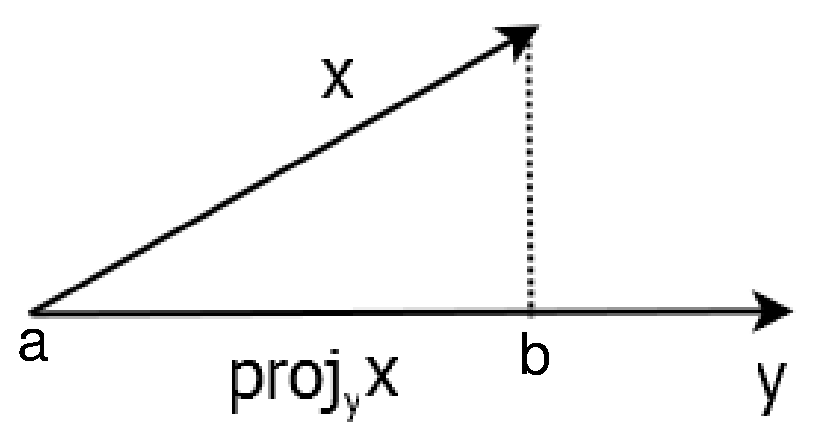
\includegraphics[width=0.5\linewidth]{projection}
\caption{Illustration of vector x projecting on vector y. $proj_{y}x$ is the projection result, a is the two vector start point, b is the projection point.}
\label{fig:projection}
\end{figure}

\section{Gaussian}
1 dimension Gaussian probability density function, defined as Eq.~\ref{equ:dimension1GaussianPDF}.

\begin{equation}
\label{equ:dimension1GaussianPDF}
\begin{aligned}
p\left( x \right) &= {\left( {2\pi } \right)^{ - \frac{1}{2}}}{\left( {{\sigma ^2}} \right)^{ - \frac{1}{2}}}\exp \left\{ { - \frac{1}{2}\left( {x - u} \right){{\left( {{\sigma ^2}} \right)}^{ - 1}}\left( {x - u} \right)} \right\}\\
 &= \frac{1}{{\sqrt {2\pi } \sigma }}\exp \left\{ { - \frac{{{{\left( {x - u} \right)}^2}}}{{2{\sigma ^2}}}} \right\}
\end{aligned}
\end{equation}
Where $x$ is variable value, $\sigma$ is the standard deviation and $u$ is the mean value. The PDF of standardized normal distribution can be defined as follow Eq.~\ref{equ:standardizedNormalDistribution}.

\begin{equation}
\label{equ:standardizedNormalDistribution}
\begin{aligned}
p\left( x \right) = \frac{1}{{\sqrt {2\pi } }}\exp \left( { - \frac{{{x^2}}}{2}} \right)
\end{aligned}
\end{equation}

Multivariate Gaussian probability density function, defined as Eq.~\ref{equ:multipleDimensionGaussianPDF}.

\begin{equation}
\label{equ:multipleDimensionGaussianPDF}
\begin{aligned}
p\left( x \right) = {\left( {2\pi } \right)^{ - \frac{d}{2}}}|\Sigma {|^{ - \frac{1}{2}}}\exp \left\{ { - \frac{1}{2}\left( {x - u} \right){\Sigma ^{ - 1}}{{\left( {x - u} \right)}^t}} \right\}
\end{aligned}
\end{equation}
Where $d$ is the dimension of variable $x$, $\Sigma$ is the variance matrix (covariance matrix) and $u$ is the vector of mean value.

The log derivation of multivariate Gaussian probability function can be computed by Eq.~\ref{equ:gaussianDerivation}.

\begin{equation}
\label{equ:gaussianDerivation}
\begin{aligned}
\log p\left( x \right) &=  - \frac{d}{2}\log 2\pi  - \frac{1}{2}\log |\Sigma | - \frac{1}{2}\left( {x - u} \right){\Sigma ^{ - 1}}{\left( {x - u} \right)^t}\\
\frac{{\partial \log p\left( x \right)}}{{\partial u}} &=  - \left( {x - u} \right){\Sigma ^{ - 1}}\\
\frac{{\partial \log p\left( x \right)}}{{\partial {\Sigma ^{ - 1}}}} &= \frac{{\partial \left( { - \frac{1}{2}\log |\Sigma | - \frac{1}{2}\left( {x - u} \right){\Sigma ^{ - 1}}{{\left( {x - u} \right)}^t}} \right)}}{{\partial {\Sigma ^{ - 1}}}}\\
 &= \frac{{\partial \left( { - \frac{1}{2}\log |{\Sigma ^{ - 1}}{|^{ - 1}} - \frac{1}{2}\left( {x - u} \right){\Sigma ^{ - 1}}{{\left( {x - u} \right)}^t}} \right)}}{{\partial {\Sigma ^{ - 1}}}}\\
 &= \frac{{\partial \left( {\frac{1}{2}\log |{\Sigma ^{ - 1}}| - \frac{1}{2}\left( {x - u} \right){\Sigma ^{ - 1}}{{\left( {x - u} \right)}^t}} \right)}}{{\partial {\Sigma ^{ - 1}}}}\\
 &= \frac{1}{2}\frac{1}{{|{\Sigma ^{ - 1}}|}}|{\Sigma ^{ - 1}}|{\left( {{\Sigma ^{ - 1}}} \right)^{ - 1}} - \frac{1}{2}{\left( {x - u} \right)^t}\left( {x - u} \right)\\
 &= \frac{1}{2}\Sigma  - \frac{1}{2}{\left( {x - u} \right)^t}\left( {x - u} \right)
\end{aligned}
\end{equation}

\section{Matrix}

\subsection{Matrix Operation}
Let $m$ denotes a square matrix, $n$ denotes the algebraic complement of $m$, ${{m^ \circ }}$ denotes the companion matrix of $m$, $s$ denotes the size of $m$. $U$ denotes the unit matrix. Then we have Eq.~\ref{equ:matrixCompanion}.

\begin{equation}
\label{equ:matrixCompanion}
\begin{aligned}
{m^ \circ } &= \left[ {\begin{array}{*{20}{c}}
{{n_{00}}}&{...}&{{n_{s - 1,0}}}\\
{...}&{...}&{...}\\
{{n_{0,s - 1}}}&{...}&{{n_{s - 1,s - 1}}}
\end{array}} \right]\\
{m^{ - 1}} &= \frac{{{m^ \circ }}}{{|m|}}\\
m{m^ \circ } &= {m^ \circ }m = |m|U\\
{\left( {{m^{ - 1}}} \right)^{ - 1}} &= m\\
{\left( {{m^n}} \right)^{ - 1}} &= {\left( {{m^{ - 1}}} \right)^n}\\
{\left( {km} \right)^{ - 1}} &= \frac{1}{k}{m^{ - 1}},\ \left( {{\rm{k\ is\ no\ zero\ value}}} \right)\\
{\left( {{m^{*0}}{m^{*1}}...{m^{*n}}} \right)^{ - 1}} &= {\left( {{m^{*n}}} \right)^{ - 1}}...{\left( {{m^{*1}}} \right)^{ - 1}}{\left( {{m^{*0}}} \right)^{ - 1}}
\end{aligned}
\end{equation}

For the determinant of square matrices $a$ and $b$, we have Eq.~\ref{equ:matrixDeterminant}.

\begin{equation}
\label{equ:matrixDeterminant}
\begin{aligned}
&|ab| = |a||b|\\
\Rightarrow& |a{a^{ - 1}}| = |a||{a^{ - 1}}| = 1\\
 \Rightarrow& |a| = |{a^{ - 1}}{|^{ - 1}}
\end{aligned}
\end{equation}

\subsection{Matrix Derivation}
A derivation of value for matrix shows as Eq.~\ref{equ:valueDerivationMatrix}.
\begin{equation}
\label{equ:valueDerivationMatrix}
\begin{aligned}
\frac{{\partial A}}{{\partial w}} = \begin{bmatrix}
{\frac{{\partial A}}{{\partial {w_{00}}}}}&{..}&{\frac{{\partial A}}{{\partial {w_{0,m - 1}}}}} \\
{..}&{..}&{..} \\
{\frac{{\partial A}}{{\partial {w_{n - 1, 0}}}}}&{..}&{\frac{{\partial A}}{{\partial {w_{n - 1, m - 1}}}}}
\end{bmatrix}
\end{aligned}
\end{equation}

Let $w$ denotes $1 \times n$ matrix, $a$ denotes $n \times n$ matrix, then we have Eq.~\ref{equ:matrixTransposition}.
\begin{equation}
\label{equ:matrixTransposition}
\begin{aligned}
&f(w) = w{w^t},\frac{{\partial f}}{{\partial w}} = 2w\\
&f(w) = wa{w^t},\frac{{\partial f}}{{\partial w}} = 2wa\\
&f(a) = wa{w^t}, \frac{{\partial f}}{{\partial a}} = w^tw\\
\end{aligned}
\end{equation}

Let $m$ denotes square matrix, $n$ denotes the algebraic complement of $m$, $m^{\circ}$ denotes the companion matrix of $m$. Then we have Eq.~\ref{equ:matrixDetDerivation} for the derivation of the determinant of square matrices $m$ about $m$ and $m^{-1}$.

\begin{equation}
\label{equ:matrixDetDerivation}
\begin{aligned}
\frac{{\partial |m|}}{{\partial m}} &= \left[ {\begin{array}{*{20}{c}}
{\frac{{\partial |m|}}{{\partial {m_{00}}}}}&{...}&{\frac{{\partial |m|}}{{\partial {m_{0,s - 1}}}}}\\
{...}&{...}&{...}\\
{\frac{{\partial |m|}}{{\partial {m_{s - 1,0}}}}}&{...}&{\frac{{\partial |m|}}{{\partial {m_{s - 1,s - 1}}}}}
\end{array}} \right]\\
 &= \left[ {\begin{array}{*{20}{c}}
{\frac{{\partial \sum\limits_{i = 0}^{s - 1} {{m_{0i}}{n_{0i}}} }}{{\partial {m_{00}}}}}&{...}&{\frac{{\partial \sum\limits_{i = 0}^{s - 1} {{m_{0i}}{n_{0i}}} }}{{\partial {m_{0,s - 1}}}}}\\
{...}&{...}&{...}\\
{\frac{{\partial \sum\limits_{i = 0}^{s - 1} {{m_{s - 1,i}}{n_{0i}}} }}{{\partial {m_{s - 1,0}}}}}&{...}&{\frac{{\partial \sum\limits_{i = 0}^{s - 1} {{m_{s - 1,i}}{n_{0i}}} }}{{\partial {m_{s - 1,s - 1}}}}}
\end{array}} \right]\\
 &= \left[ {\begin{array}{*{20}{c}}
{{n_{00}}}&{...}&{{n_{0,s - 1}}}\\
{...}&{...}&{...}\\
{{n_{s - 1,0}}}&{...}&{{n_{s - 1,s - 1}}}
\end{array}} \right]\\
 &= {\left( {{m^ \circ }} \right)^t}\\
 &= {\left( {|m|{m^{ - 1}}} \right)^t}\\
 &= |m|{m^{ - t}}\\
\frac{{\partial |m|}}{{\partial {m^{ - 1}}}} &= \frac{{\partial |m|}}{{\partial |{m^{ - 1}}|}}\frac{{\partial |{m^{ - 1}}|}}{{\partial {m^{ - 1}}}}\\
 &= \frac{{\partial |{m^{ - 1}}{|^{ - 1}}}}{{\partial |{m^{ - 1}}|}}\frac{{\partial |{m^{ - 1}}|}}{{\partial {m^{ - 1}}}}\\
 &=  - |{m^{ - 1}}{|^{ - 2}}|{m^{ - 1}}|{m^t}\\
 &=  - |{m^{ - 1}}{|^{ - 1}}{m^t}\\
 &=  - |m|{m^t}
\end{aligned}
\end{equation}

\subsection{Advance}

\begin{theorem}[The diagonal conservation of Real symmetric matrix]
\label{the:diagonalConservation}
Given a real symmetric matrix $m$, a normal orthogonal matrix $w$, we have the Eq.~\ref{equ:diagonalConservation}.

\begin{equation}
\label{equ:diagonalConservation}
\sum\limits_{i = 0}^{D - 1} {{m_{ii}}}  = \sum\limits_{i = 0}^{D - 1} {{w^t}mw}  = \sum\limits_{i = 0}^{D - 1} {wm{w^t}} 
\end{equation}

\end{theorem}

\section{Convolution Operation}
A common convolution function can be described by Eq.~\ref{equ:baseConv}.
\begin{equation}
\label{equ:baseConv}
h(x) = (f \otimes k)(x) = \int_{ - \infty }^\infty  {f(x - t)k(t)dt = } \int_{ - \infty }^\infty  {f(t)k(x - t)dt}
\end{equation}

In 2d image (all variables are discrete), the convolution can be described as below process.
\begin{itemize}
  \item Rotate the kernel with 180 degree,
  \item Move the kernel step by step accord the constraint,
  \item Add the product value of corresponding points, and the value is one convolution result.
\end{itemize}

The convolution operation has three types, full, valid and same, as shown in Fig.~\ref{fig:convType}. We first define image accessing function $f$ as Eq.~\ref{equ:imageAccessing}.
\begin{equation}
\label{equ:imageAccessing}
f(i, j) = \left\{
\begin{aligned}
&f(i, j),(i, j) \in image\\
&0,(i, j) \notin image
\end{aligned}
\right.
\end{equation}

Let denote the $x$ is source image, $k$ is the convolution kernel, $y$ is the convolution result, $w_k,h_k$ are the width and height of kernel, $w_x, h_x$ are the width and height of source image, $w_y, h_y$ are the width and height of result. The formula of valid type is shown as Eq.~\ref{convValid}.

\begin{figure}
\centering
\includegraphics[width=0.8\linewidth]{convType}
\caption{Illustration of three type of convolution. (a) full, (b) valid, (c) same for odd kernel and (d) same for even kernel. From the picture, we can see that the kernel must has at least one point intersected with source image in the full type, while the kernel must in source image totally in the valid type and the center of the kernel must in source image in the same type. All the three types, the center of every moved kernel correspond to a point of destination image.}
\label{fig:convType}
\end{figure}

\begin{equation}
\label{convFull}
\begin{aligned}
y(i,j) &= \sum\limits_{m,n} {x(i - m,j - n)k(m,n)}\\
size(y) &= size(x) + size(k) - 1
\end{aligned}
\end{equation}

\begin{equation}
\label{convValid}
\begin{aligned}
y(i,j) &= \sum\limits_{m,n} {x(i + k_{*h} - 1 - m,j + k_{*w} - 1 - n)k(m,n)}\\
size(y) &= size(x) - size(k) + 1
\end{aligned}
\end{equation}

\begin{equation}
\label{convSame}
\begin{aligned}
y(i,j) &= \sum\limits_{m,n} {x(i + \frac{k_{*h}}{2} - m,j + \frac{k_{*w}}{2} - n)k(m,n)}\\
size(y) &= size(x)
\end{aligned}
\end{equation}
Where $(i, j) \in y$, $m, n\in [ -\infty,...,+\infty]$ and $x, k$ all satisfy $f$.

There is other representation of convolution. For full type, we have Eq.~\ref{equ:convFullOther}. 

\begin{equation}
\label{equ:convFullOther}
\begin{aligned}
y(i,j) &= \sum\limits_{m,n} {x(i - m,j - n)k(m,n)} \\
&{\text{Let }p = i - m,q = j - n}\\
y(i,j) &= \sum\limits_{i - p,j - q} {x(p,q)k(i - p,j - q)}\\
 &= \sum\limits_{p,q} {x(p,q)k(i - p,j - q)} 
\end{aligned}
\end{equation}

In like manner, we have Eq.~\ref{equ:convValidOther} for valid type and Eq.~\ref{equ:convSameOther} for same type. $p, q \in [ -\infty,...,+\infty]$ in all of them.

\begin{equation}
\label{equ:convValidOther}
\begin{aligned}
y(i,j) &= \sum\limits_{m,n} {x(i + k_{*h} - 1 - m,j + k_{*w} - 1 - n)k(m,n)} \\
&{\text{Let }}p = i + k_{*h} - 1 - m,{\rm{ }}q{\rm{ =  }}j + k_{*k} - 1 - n\\
y(i,j) &= \sum\limits_{p,q} {x(p,q)k(i + k_{*h} - 1 - p,j + k_{*w} - 1 - q)} 
\end{aligned}
\end{equation}

\begin{equation}
\label{equ:convSameOther}
\begin{aligned}
y(i,j){\rm{ }} &= \sum\limits_{m,n} {x(i + \frac{k_{*h}}{2} - m,j + \frac{k_{*w}}{2} - n)k(m,n)} \\
&{\text{Let }}p = i + \frac{k_{*h}}{2} - m,{\rm{ }}q{\rm{ =  }}j + \frac{k_{*w}}{2} - n\\
y(i,j) &= \sum\limits_{p,q} {x(p,q)k(i + \frac{k_{*h}}{2} - p,j + \frac{k_{*w}}{2}  - q)} 
\end{aligned}
\end{equation}

To handle the different orientation of source image and kernel, here are three equation table for different type of convolution operation in different angle.

\begin{table}[t]
\newcommand{\tabincell}[2]{\begin{tabular}{@{}#1@{}}#2\end{tabular}}
\begin{center}
\caption{Full Convolution equations} \label{tab:euqationFullConv}
\begin{tabular}{|l|c|}
  \hline
  Function & Equation\\
  \hline
  $x \otimes k$ & \tabincell{c}{$y(i,j) = \sum\limits_{m,n} {x(i - m,j - n)k(m,n)}$\\$y(i,j) = \sum\limits_{p,q} {x(p,q)k(i - p,j - q)} $} \\
  \hline
  $x \otimes k^{180}$ & \tabincell{c}{$y(i,j) = \sum\limits_{m,n} {x(i - k_{*h} + 1 + m, j - k_{*w} + 1+ n)k(m,n)}$\\$y(i,j) = \sum\limits_{p,q} {x(p, q)k(p + k_{*h} - 1 - i, q + k_{*w} - 1 - j)}$}\\
  \hline  
  $x^{180} \otimes k$ & \tabincell{c}{$y(i,j) = \sum\limits_{m,n} {x(x_{*h} - 1 - i + m, k_{*w} - 1 - j + n)k(m,n)}$\\$y(i,j) = \sum\limits_{p,q} {x(p, q)k(p - k_{*h} + 1 + i, q - k_{*w} + 1 + j)}$}\\
  \hline  
\end{tabular}
\end{center}
\end{table}

\begin{table}[t]
\newcommand{\tabincell}[2]{\begin{tabular}{@{}#1@{}}#2\end{tabular}}
\begin{center}
\caption{Same Convolution equations} \label{tab:euqationSameConv}
\begin{tabular}{|l|c|}
  \hline
  Function & Equation\\
  \hline
  $x \otimes k$ & \tabincell{c}{$y\left( {i,j} \right) = \sum\limits_{m,n} {x\left( {i + \frac{{{k_{*h}}}}{2} - m,j + \frac{{{k_{*w}}}}{2} - n} \right)k\left( {m,n} \right)} $ \\$y\left( {i,j} \right) = \sum\limits_{p,q} {x\left( {p,q} \right)k\left( {i + \frac{{{k_{*h}}}}{2} - p,j + \frac{{{k_{*w}}}}{2} - q} \right)} $} \\
  \hline
  $x \otimes k^{180}$ & \tabincell{c}{$y\left( {i,j} \right) = \sum\limits_{m,n} {x\left( {i - \frac{{{k_{*h}}} - 1}{2} + m,j - \frac{{{k_{*w}}} - 1}{2} + n} \right)k\left( {m,n} \right)} $\\$y\left( {i,j} \right) = \sum\limits_{p,q} {x\left( {p,q} \right)k\left( {p + \frac{{{k_{*h}}} - 1}{2} - i,q + \frac{{{k_{*w}}} - 1}{2} - j} \right)} $}\\
  \hline  
  $x^{180} \otimes k$ & \tabincell{c}{$y\left( {i,j} \right) = \sum\limits_{m,n} {x\left( {{x_{*h}} - 1 - i - \frac{{{k_{*h}}}}{2} + m,{x_{*w}} - j - \frac{{{k_{*w}}}}{2} + n} \right)k\left( {m,n} \right)} $\\$y\left( {i,j} \right) = \sum\limits_{p,q} {x\left( {p,q} \right)k\left( {p - {x_{*h}} + 1 + i + \frac{{{k_{*h}}}}{2},q - {x_{*w}} + 1 + j + \frac{{{k_{*w}}}}{2}} \right)} $}\\
  \hline  
\end{tabular}
\end{center}
\end{table}

\begin{table}[t]
\newcommand{\tabincell}[2]{\begin{tabular}{@{}#1@{}}#2\end{tabular}}
\begin{center}
\caption{Valid Convolution equations} \label{tab:euqationValidConv}
\begin{tabular}{|l|c|}
  \hline
  Function & Equation\\
  \hline
  $x \otimes k$ & \tabincell{c}{$y(i,j) = \sum\limits_{m,n} {x(i + k_{*h} - 1 - m,j + k_{*w} - 1 - n)k(m,n)}$\\$y(i,j) = \sum\limits_{p,q} {x(p,q)k(i + k_{*h} - 1 - p,j + k_{*w} - 1 - q)} $} \\
  \hline
  $x \otimes k^{180}$ &  \tabincell{c}{$y(i,j) = \sum\limits_{m,n} {x(i + m, j + n)k(m,n)}$\\$y(i,j) = \sum\limits_{p,q} {x(p, q)k(p - i, q - j)}$}	\\
  \hline
  $x^{180} \otimes k$ & \tabincell{c}{$y(i,j) = \sum\limits_{m,n} {x(y_{*h} - 1 - i + m, y_{*w} - 1 -j + n)k(m,n)}$\\$y(i,j) = \sum\limits_{p,q} {x(p, q)k(p - k_{*h} + 1 + i, q - k_{*w} + 1 + j)}$} \\
  \hline  
\end{tabular}
\end{center}
\end{table}

\section{Correlation Operation}
A common correlation function can be described by Eq.~\ref{equ:baseCorr}.
\begin{equation}
\label{equ:baseCorr}
h\left( x \right) = (f \odot k)\left( x \right) = \int_{ - \infty }^\infty  {f(x + t)k(t)dt = } \int_{ - \infty }^\infty  {f(t)k(x + t)dt} 
\end{equation}

Similar to the convolution operation, we directly give the equations as following.
Correlation for full, valid and same type are defined as Eq.~\ref{corr_full}, Eq.~\ref{corr_valid} and Eq.~\ref{corr_same}.

\begin{equation}
\label{corr_full}
\begin{aligned}
y(i,j) &= \sum\limits_{m,n} {x(i - {k_{*w}} + 1 + m,j - {k_{*h}} + 1 + n)k(m,n)} \\
y(i,j) &= \sum\limits_{p,q} {x(p,q)k(p - i + {k_{*w}} - 1,q - j + {k_{*h}} - 1)} \\
size(y) &= size(x) + size(k) - 1
\end{aligned}
\end{equation}

\begin{equation}
\label{corr_valid}
\begin{aligned}
y(i,j) &= \sum\limits_{m,n} {x(i + m,j + n)k(m,n)} \\
y(i,j) &= \sum\limits_{p,q} {x(p,q)k(p - i,q - j)} \\
size(y) &= size(x) - size(k) + 1
\end{aligned}
\end{equation}

\begin{equation}
\label{corr_same}
\begin{aligned}
y(i,j) &= \sum\limits_{m,n} {x(i - \frac{{{k_{*w}} - 1}}{2} + m,j - \frac{{{k_{*h}} - 1}}{2} + n)k(m,n)} \\
y(i,j) &= \sum\limits_{p,q} {x(p,q)k(p - i + \frac{{{k_{*w}} - 1}}{2},q - j + \frac{{{k_{*h}} - 1}}{2})} \\
size(y) &= size(x)
\end{aligned}
\end{equation}
Where $(i, j) \in y$, $m, n\in [ -\infty,...,+\infty]$ and $x, k$ all satisfy $f$.

To handle the different orientation of source image and kernel, here are three equation table for different type of convolution operation in different angle.

\begin{table}[t]
\newcommand{\tabincell}[2]{\begin{tabular}{@{}#1@{}}#2\end{tabular}}
\begin{center}
\caption{Full Correlation equations} \label{tab:euqationFullCorr}
\begin{tabular}{|l|c|}
  \hline
  Function & Equation\\
  \hline
  $x \odot k$ & \tabincell{c}{$y(i,j) = \sum\limits_{m,n} {x(i - {k_{*h}} + 1 + m,j - {k_{*w}} + 1 + n)k(m,n)}$\\$y(i,j) = \sum\limits_{p,q} {x(p,q)k(p - i + {k_{*h}} - 1,q - j + {k_{*w}} - 1)} $} \\
  \hline
  $x \odot k^{180}$ & \tabincell{c}{$y(i,j) = \sum\limits_{m,n} {x(i - m,j - n)k(m,n)}$\\$y(i,j) = \sum\limits_{p,q} {x(p,q)k(i - p,j - q)} $}\\
  \hline  
  $x^{180} \odot k$ & \tabincell{c}{$y(i,j) = \sum\limits_{m,n} {x({y_{*h}} - i - 1 - m,{y_{*w}} - j - 1 - n)k(m,n)}$\\$y(i,j) = \sum\limits_{p,q} {x(p,q)k({y_{*h}} - i - 1 - p,{y_{*w}} - j - 1 - q)}$}\\
  \hline  
\end{tabular}
\end{center}
\end{table}

\begin{table}[t]
\newcommand{\tabincell}[2]{\begin{tabular}{@{}#1@{}}#2\end{tabular}}
\begin{center}
\caption{Same Correlation equations} \label{tab:euqationSameCorr}
\begin{tabular}{|l|c|}
  \hline
  Function & Equation\\
  \hline
  $x \odot k$ & \tabincell{c}{$y\left( {i,j} \right) = \sum\limits_{m,n} {x\left( {i - \frac{{{k_{*h}}} - 1}{2} + m,j - \frac{{{k_{*w}}} - 1}{2} + n} \right)k\left( {m,n} \right)} $\\$y\left( {i,j} \right) = \sum\limits_{p,q} {x\left( {p,q} \right)k\left( {p + \frac{{{k_{*h}}} - 1}{2} - i,q + \frac{{{k_{*w}}} - 1}{2} - j} \right)} $} \\
  \hline
  $x \odot k^{180}$ & \tabincell{c}{$y\left( {i,j} \right) = \sum\limits_{m,n} {x\left( {i + \frac{{{k_{*h}}}}{2} - m,j + \frac{{{k_{*w}}}}{2} - n} \right)k\left( {m,n} \right)} $ \\$y\left( {i,j} \right) = \sum\limits_{p,q} {x\left( {p,q} \right)k\left( {i + \frac{{{k_{*h}}}}{2} - p,j + \frac{{{k_{*w}}}}{2} - q} \right)} $}\\
  \hline  
  $x^{180} \odot k$ & \tabincell{c}{$y(i,j) = \sum\limits_{m,n} {x({x_{*h}} - 1 - i + \frac{{{k_{*w}} - 1}}{2} - m,{x_{*w}} - 1 - j + \frac{{{k_{*h}} - 1}}{2} - n)k(m,n)}$\\$y(i,j) = \sum\limits_{p,q} {x(p,q)k({x_{*h}} - 1 - i + \frac{{{k_{*w}} - 1}}{2} - p,{x_{*w}} - 1 - j + \frac{{{k_{*h}} - 1}}{2} - q)}$}\\
  \hline  
\end{tabular}
\end{center}
\end{table}

\begin{table}[t]
\newcommand{\tabincell}[2]{\begin{tabular}{@{}#1@{}}#2\end{tabular}}
\begin{center}
\caption{Valid Correlation equations} \label{tab:euqationValidCorr}
\begin{tabular}{|l|c|}
  \hline
  Function & Equation\\
  \hline
  $x \odot k$ & \tabincell{c}{$y(i,j) = \sum\limits_{m,n} {x(i + m, j + n)k(m,n)}$\\$y(i,j) = \sum\limits_{p,q} {x(p, q)k(p - i, q - j)}$} \\
  \hline
  $x \odot k^{180}$ &  \tabincell{c}{$y(i,j) = \sum\limits_{m,n} {x(i + k_{*h} - 1 - m,j + k_{*w} - 1 - n)k(m,n)}$\\$y(i,j) = \sum\limits_{p,q} {x(p,q)k(i + k_{*h} - 1 - p,j + k_{*w} - 1 - q)} $}	\\
  \hline
  $x^{180} \odot k$ & \tabincell{c}{$y(i,j) = \sum\limits_{m,n} {x({x_{*h}} - 1 - i - m,{x_{*w}} - 1 - j - n)k(m,n)} $\\$y(i,j) = \sum\limits_{p,q} {x(p,q)k({x_{*h}} - 1 - i - p,{x_{*w}} - 1 - j - q)}$} \\
  \hline  
\end{tabular}
\end{center}
\end{table}

The following equations are the other relations between convolution and correlation.

\begin{equation}
\label{equ:x_180_conv_y_relation_to_correlation}
\begin{aligned}
{\left( {{x^{180}} \otimes k} \right)^{180}} &= {y^{180}}\left( {i,j} \right) = y\left( {{i^{'}},{j^{'}}} \right)\\
 &= y\left( {{y_{*h}} - 1 - i,{y_{*w}} - 1 - j} \right)\\
 &= \sum\limits_{m,n} {x({x_{*h}} - 1 - {i^{'}} + m,{x_{*w}} - 1 - {j^{'}} + n)k(m,n)} \\
 &= \sum\limits_{m,n} {x({x_{*h}} - 1 - \left( {{y_{*h}} - 1 - i} \right) + m,{x_{*w}} - 1 - \left( {{y_{*w}} - 1 - j} \right) + n)k(m,n)} \\
 &= \sum\limits_{m,n} {x(i - {k_{*h}} + 1 + m,j - {k_{*w}} + 1 + n)k(m,n)} \\
 &= x \odot k
\end{aligned}
\end{equation}

\section{Markov and Chebyshev Inequalities}
For a non-negative variable $x$, if its expectation exist, the we have the Markov inequality as Eq.~\ref{equ:markovChebyshevMarkov}.

\begin{equation}
\label{equ:markovChebyshevMarkov}
P\left( {x \ge \varepsilon } \right) \le \frac{{E\left( x \right)}}{\varepsilon }
\end{equation}
Where $\varepsilon$ is a positive value.

If the variance of $x$ is existent, then we have the Chebyshev inequality through the following derivation as Eq.~\ref{equ:markovChebyshevChebyshev}.

\begin{equation}
\label{equ:markovChebyshevChebyshev}
\begin{aligned}
&P\left( {|x - E\left( x \right)| \ge \varepsilon } \right) = P\left( {{{\left( {x - E\left( x \right)} \right)}^2} \ge {\varepsilon ^2}} \right) \le \frac{{E\left( {{{\left( {x - E\left( x \right)} \right)}^2}} \right)}}{{{\varepsilon ^2}}}\\
 \Rightarrow &P\left( {|x - E\left( x \right)| \ge \varepsilon } \right) \le \frac{{E{x^2} - {E^2}\left( x \right)}}{{{\varepsilon ^2}}}\\
 \Rightarrow &P\left( {|x - E\left( x \right)| \ge \varepsilon } \right) \le \frac{{Dx}}{{{\varepsilon ^2}}}
\end{aligned}
\end{equation}

We can roughly give a upper bound for an event through the Markov and Chebyshev inequalities. Since the Chebyshev inequality exploit both expectation and variance, so it is more accurate than Markov inequality.

\section{Law of Large Numbers}
Law of large numbers is a law to describe the probabilistic property on the large times of experiment. The average value of random variable will approximate to the expectation in the increased times of experiment.

\subsection{Law of Large Numbers of Chebyshev}
Let $x^{*0}, x^{*1}, ... , x^{*K-1}$ denote the independent random variables (satisfying the same distribution is not needed), if the expectation and variance of all the variables exist, then we have Eq.~\ref{equ:lawOfLargeOfChebyshev}. 

\begin{equation}
\label{equ:lawOfLargeOfChebyshev}
\begin{aligned}
&\mathop {\lim }\limits_{N \to \infty } p\left( {|\frac{1}{N}\sum\limits_{i = 0}^{N - 1} {{x^{*i}}}  - \frac{1}{N}\sum\limits_{i = 0}^{N - 1} {E\left( {{x^{*i}}} \right)} | < \varepsilon } \right) = 1\\
 \sim &N \to \infty ,\frac{1}{n}\sum\limits_{i = 0}^{N - 1} {{x^{*i}}}  = \frac{1}{N}\sum\limits_{i = 0}^{N - 1} {E\left( {{x^{*i}}} \right)} 
\end{aligned}
\end{equation}
Where $N$ is the count of variable $x$, $\varepsilon$ is any value bigger that 0.

\subsection{Law of Large Numbers of Khinchine}
\label{sec:lawOfLargeKhinchine}
Let $x$ denotes a random variable, $x^{*i}$ is the $ith$ data sampled randomly from the distribution that $x$ satisfy, then we have Eq.~\ref{equ:lawOfLargeOfKhinchine}.

\begin{equation}
\label{equ:lawOfLargeOfKhinchine}
\begin{aligned}
&\mathop {\lim }\limits_{N \to \infty } p\left( {|\frac{1}{N}\sum\limits_{i = 0}^{N - 1} {{x^{*i}}}  - E\left( x \right)| < \varepsilon } \right) = 1\\
 \sim &N \to \infty ,E\left( x \right) = \frac{1}{N}\sum\limits_{i = 0}^{N - 1} {{x^{*i}}} 
\end{aligned}
\end{equation}
Where $\varepsilon$ is any value bigger that 0.

Here we give the proof of law of Large number of Khinchine in continuous random variable. Since the expectation of multivariate variable can be independently calculated in each dimension, we can only prove the law in 1-d data. We exploit the kernel density estimation with uniform kernel function to estimate the probability value, as shown in Eq.~\ref{equ:lawOfLargeOfKDE}.

\begin{equation}
\label{equ:lawOfLargeOfKDE}
\begin{aligned}
p\left( x \right) &\approx \frac{1}{N}\sum\limits_{i = 0}^{N - 1} {\delta \left( {{x^{*i}},x} \right)} \\
\delta \left( {{x^{*i}},x} \right) &= \left\{ {\begin{array}{*{20}{c}}
{\frac{1}{r},|{x^{*i}} - x| \le \frac{r}{2}}\\
{0,otherwise}
\end{array}} \right.
\end{aligned}
\end{equation}
Where the estimation value will be more precision when $N$ becomes bigger.
Then we obtain the proof procedure as shown in Eq.~\ref{equ:lawOfLargeOfKhinchineProof}.

\begin{equation}
\label{equ:lawOfLargeOfKhinchineProof}
\begin{aligned}
E\left( x \right) &= \int\limits_x {p\left( x \right)xdx} \\
 &\approx \int\limits_x {\frac{1}{N}\sum\limits_{i = 0}^{N - 1} {\delta \left( {{x^{*i}},x} \right)} xdx} \\
 &= \frac{1}{N}\int\limits_x {\sum\limits_{i = 0}^{N - 1} {\delta \left( {{x^{*i}},x} \right)} xdx} \\
 &= \frac{1}{N}\sum\limits_{i = 0}^{N - 1} {\int\limits_x {\delta \left( {{x^{*i}},x} \right)xdx} } \\
 &= \frac{1}{N}\sum\limits_{i = 0}^{N - 1} {\left( {\int\limits_{|{x^{*i}} - x| \le \frac{r}{2}} {\delta \left( {{x^{*i}},x} \right)xdx}  + \int\limits_{|{x^{*i}} - x| > \frac{r}{2}} {\delta \left( {{x^{*i}},x} \right)xdx} } \right)} \\
 &= \frac{1}{N}\sum\limits_{i = 0}^{N - 1} {\left( {\frac{1}{r}\int\limits_{|{x^{*i}} - x| \le \frac{r}{2}} {xdx} } \right)} \\
 &= \frac{1}{N}\sum\limits_{i = 0}^{N - 1} {\left( {\frac{1}{r}\frac{{{x^2}}}{2}|\begin{array}{*{20}{c}}
{{x^{*i}} + \frac{r}{2}}\\
{{x^{*i}} - \frac{r}{2}}
\end{array}} \right)} \\
 &= \frac{1}{N}\sum\limits_{i = 0}^{N - 1} {\left( {\frac{1}{r}\frac{{{{\left( {{x^{*i}} + \frac{r}{2}} \right)}^2} - {{\left( {{x^{*i}} - \frac{r}{2}} \right)}^2}}}{2}} \right)} \\
 &= \frac{1}{N}\sum\limits_{i = 0}^{N - 1} {{x^{*i}}} 
\end{aligned}
\end{equation}

Actually, we can assume that $x^{*i} \approx x$ in the range of $x \in {|{x^{*i}} - x| \le \frac{r}{2}}$, thus the proof can be simply by the Eq.~\ref{equ:lawOfLargeOfKhinchineProofSimply}.

\begin{equation}
\label{equ:lawOfLargeOfKhinchineProofSimply}
\begin{aligned}
E\left( x \right) &\approx \frac{1}{n}\sum\limits_{i = 0}^{N - 1} {\left( {\frac{1}{r}\int\limits_{|{x^{*i}} - x| \le \frac{r}{2}} {xdx} } \right)} \\
 &\approx \frac{1}{N}\sum\limits_{i = 0}^{N - 1} {\left( {\frac{1}{r}x^{*i}r} \right)} \\
 &= \frac{1}{N}\sum\limits_{i = 0}^{N - 1} {{x^{*i}}} 
\end{aligned}
\end{equation}

Similarly, we can apply the law for computing the expectation of function, as shown in Eq.~\ref{equ:lawOfLargeOfKhinchineForFunction}.

\begin{equation}
\label{equ:lawOfLargeOfKhinchineForFunction}
\begin{aligned}
E\left( {f\left( x \right)} \right) &= \int\limits_x {p\left( x \right)f\left( x \right)dx} \\
 &\approx \frac{1}{N}\sum\limits_{i = 0}^{N - 1} {\left( {\frac{1}{r}f\left( {{x^{*i}}} \right)r} \right)} \\
 &= \frac{1}{N}\sum\limits_{i = 0}^{N - 1} {f\left( {{x^{*i}}} \right)} 
\end{aligned}
\end{equation}
Where we assume that $f\left(x^{*i}\right) \approx f\left(x\right)$ in the range of $x \in {|{x^{*i}} - x| \le \frac{r}{2}}$. This is the basis of the Monte Carlo method.

\subsection{Law of Large Numbers of Bernoulli}
Law of large numbers of Bernoulli is a special case of Law of Large Numbers of Khinchine that the variable is binary type, 0 or 1. If we define the variable 1 means the occurrence of an event, the expectation can be considered the probability of the occurrence of an event. Then we have Eq.~\ref{equ:lawOfLargeOfBernoulli}.

\begin{equation}
\label{equ:lawOfLargeOfBernoulli}
\begin{aligned}
&\mathop {\lim }\limits_{N \to \infty } p\left( {|\frac{C}{N} - \tilde p| < \varepsilon } \right) = 1\\
 \sim &N \to \infty ,\tilde p = \frac{C}{N}
\end{aligned}
\end{equation}
Where $C$ is the number of occurrence of an event in $n$ times experiments, $\tilde{p}$ is the probability of the occurrence of the event, $\varepsilon$ is any value bigger that 0.

\subsection{Law of Large Numbers of Mean Approximation}
For different random variables $x^{*0}, x^{*1}, ..., x^{*N-1}$ and different approximate linear functions \\
$f^{*0}, f^{*1}, ..., f^{*N-1}$, we have the law of large numbers of mean approximation as shown in Eq.~\ref{equ:lawOfLargeOfMeanApproximation}.

\begin{equation}
\label{equ:lawOfLargeOfMeanApproximation}
\begin{aligned}
\sum\limits_{i = 0}^{N - 1} {{f^{*i}}\left( {{{\tilde x}^{*i}}} \right)}  \approx \sum\limits_{i = 0}^{N - 1} {{f^{*i}}\left( {E\left( {{x^{*i}}} \right)} \right)}  \approx \sum\limits_{i = 0}^{N - 1} {E\left( {{f^{*i}}\left( {{x^{*i}}} \right)} \right)} 
\end{aligned}
\end{equation}
Where $\tilde x^{*i}$ is a sample sampled from $p\left(x^{*i}\right)$.

Consider the special case of the above law (different random variables satisfy the identical distribution), for one random variable $x$ and one approximate linear function $f$, we have the law as shown in Eq.~\ref{equ:lawOfLargeOfMeanApproximationOneVariable}.

\begin{equation}
\label{equ:lawOfLargeOfMeanApproximationOneVariable}
f\left( {E\left( x \right)} \right) \approx \frac{1}{N}\sum\limits_{i = 0}^{N - 1} {f\left( {{x^{*i}}} \right)}  \approx E\left( {f\left( x \right)} \right)
\end{equation}
Where $x^{*i}$ is the $ith$ sample sampled from $p\left(x\right)$.

\section{Central Limit Theorem}
Suppose that random variables $x^{*0}, x^{*1},..., x^{*N-1}$ are independently sampled from the same distribution. The variance $\sigma ^ 2$ of the distribution is existent (the expectation $u$ is also existent). Then we have the central limit theorem in independent and identical distribution situation (Lindburg-Levy theorem) as Eq.~\ref{equ:centralLimitTheoremLindburgLevy}.

\begin{equation}
\label{equ:centralLimitTheoremLindburgLevy}
\begin{aligned}
&\mathop {\lim }\limits_{N \to  + \infty } P\left( {\frac{1}{{\sqrt {N{\sigma ^2}} }}\left( {\sum\limits_{i = 0}^{N - 1} {{x^{*i}}}  - Nu} \right) \le x} \right) = \Phi \left( {x} \right)\\
 \sim &\frac{1}{{\sqrt {N{\sigma ^2}} }}\left( {\sum\limits_{i = 0}^{N - 1} {{x^{*i}}}  - Nu} \right) \sim N\left( {0,1} \right)\\
 \sim &\sum\limits_{i = 0}^{N - 1} {{x^{*i}}}  \sim N\left( {nu,n{\sigma ^2}} \right)
\end{aligned}
\end{equation}

Consider the random variable $x$ satisfy the 0-1 distribution $B\left(1, p\right)$. Let $y = \sum\limits_{i = 0}^{N - 1} {{x^{*i}}} $, thus $u=E\left(y\right)=np, \sigma ^ 2 = D\left(y\right)=np\left(1-p\right)$. Then we have the Eq.~\ref{equ:centralLimitTheoremMovireLaplace} (de Movire - Laplace theorem) that indicates the Gaussian distribution is the limit for binary distribution when $N\to  + \infty$.

\begin{equation}
\label{equ:centralLimitTheoremMovireLaplace}
\begin{aligned}
&\mathop {\lim }\limits_{N \to  + \infty } P\left( {\frac{1}{{\sqrt {Np\left( {1 - p} \right)} }}\left( {y - Np} \right) \le x} \right) = \Phi \left( x \right)\\
 \sim& \frac{1}{{\sqrt {Np\left( {1 - p} \right)} }}\left( {y - Np} \right) \sim N\left( {0,1} \right)\\
 \sim& y \sim N\left( {Np,Np\left( {1 - p} \right)} \right)
\end{aligned}
\end{equation}

We further extend the theorems to linear combination form. Consider the random variable $x^{*i}$ satisfy the 0-1 distribution $B\left(1, p\right)$. Let $y = \sum\limits_{i = 0}^{N - 1} {{\alpha ^{*i}}{x^{*i}}} $, then we have Eq.~\ref{equ:centralLimitTheorem_linear_combination_form}.

\begin{equation}
\label{equ:centralLimitTheorem_linear_combination_form}
y \sim N\left( {p\sum\limits_{i = 0}^{N - 1} {{\alpha ^{*i}}} ,p\left( {1 - p} \right)\sum\limits_{i = 0}^{N - 1} {{{\left( {{\alpha ^{*i}}} \right)}^2}} } \right)
\end{equation}

\section{Taylor's Formula}
Given a function $f\left(x\right)$, we assume that $f\left(x\right)$ has $n + 1$ order continuous derivation in range between $a$ and $b$. The Taylor' formula with Lagrange remainder term as shown in Eq.~\ref{equ:taylorFormulaWithLagrange}.

\begin{equation}
\label{equ:taylorFormulaWithLagrange}
\begin{aligned}
f\left( x \right) &= t\left( {{{\left( {x - a} \right)}^n}} \right) + R\left( {{{\left( {x - a} \right)}^n}} \right)\\
t\left( {{{\left( {x - a} \right)}^n}} \right) &= f\left( a \right) + {f^{'}}\left( a \right)\left( {x - a} \right) + ... + \frac{{{f^{(n)}}\left( a \right)}}{{n!}}{\left( {x - a} \right)^n}\\
R\left( {{{\left( {x - a} \right)}^n}} \right) &= \frac{{{f^{(N + 1)}}\left( \varepsilon  \right)}}{{\left( {n + 1} \right)!}}{\left( {x - a} \right)^{n + 1}},\ \left( {\varepsilon  = a + \theta \left( {x - a} \right),0 < \theta  < 1} \right)
\end{aligned}
\end{equation}

Now we discuss the relationship of value between $f\left( x \right)$ and $t\left( {{{\left( {x - a} \right)}^n}} \right)$. Loosely speaking, if $x \approx a$ or ${{f^{(n + 1)}}\left( \varepsilon  \right)} \approx  0$ (it means the value of $f^{\left(n\right)}\left(x\right)$ between $x$ and $a$ should be near constant), then $f\left( x \right) \approx t\left( {{{\left( {x - a} \right)}^n}} \right)$.

The remainder term can be Piano term as shown in Eq.~\ref{equ:taylorPiano}. Note that the Piano remainder only needs $f$ has $n$ derivation on $a$ and only satisfy when $x$ near $a$.

\begin{equation}
\label{equ:taylorPiano}
\begin{aligned}
f\left( x \right) &= t\left( {{{\left( {x - a} \right)}^n}} \right) + R\left( {{{\left( {x - a} \right)}^n}} \right)\\
t\left( {{{\left( {x - a} \right)}^n}} \right) &= f\left( a \right) + {f^{'}}\left( a \right)\left( {x - a} \right) + ... + \frac{{{f^{(n)}}\left( a \right)}}{{n!}}{\left( {x - a} \right)^n}\\
R\left( {{{\left( {x - a} \right)}^N}} \right) &= o\left( {{{\left( {x - a} \right)}^n}} \right),\left( {x \to a,\mathop {\lim }\limits_{x \to a} \frac{{o\left( {{{\left( {x - a} \right)}^n}} \right)}}{{{{\left( {x - a} \right)}^n}}} = 0} \right)
\end{aligned}
\end{equation}

\section{Jensen Inequality}
Let us discuss the relationship of value between $E\left( {f\left( x \right)} \right)$ and $f\left( {E\left( x \right)} \right)$, where $f\left(x\right)$ is a function that can compute second derivation and 

\begin{displaymath}
\begin{aligned}
x &= \left\{ {{x^{*0}},{x^{*1}},...,{x^{*N - 1}}} \right\}\\
E\left( {f\left( x \right)} \right) &= \sum\limits_{i = 0}^{N - 1} {p\left( {{x^{*i}}} \right)f\left( {{x^{*i}}} \right)} \\
E\left( x \right) &= \sum\limits_{i = 0}^{N - 1} {p\left( {{x^{*i}}} \right){x^{*i}}} 
\end{aligned}
\end{displaymath}
The accumulation term can be replaced by integral term. We apply the Taylor's formula to expand $f$ to Eq.~\ref{equ:jensenTaylor}.

\begin{equation}
\label{equ:jensenTaylor}
f\left( x \right) = f\left( a \right) + {f^{'}}\left( a \right)\left( {x - a} \right) + {f^{''}}\left( {a + \theta \left( {x - a} \right)} \right)\frac{{{{\left( {x - a} \right)}^2}}}{2},\theta  \in \left( {0,1} \right)
\end{equation}
Where $a$ is a point in the definition domain of $f$. Here we use the Lagrange remainder term.

Suppose that $f$ is a convex function, then we have Eq.~\ref{equ:jensenTaylorInequality}.

\begin{equation}
\label{equ:jensenTaylorInequality}
\begin{aligned}
&{f^{''}}\left( {a + \theta \left( {x - a} \right)} \right) \ge 0\\
 \Rightarrow& f\left( x \right) \ge f\left( a \right) + {f^{'}}\left( a \right)\left( {x - a} \right)
\end{aligned}
\end{equation}

According to the derivation of Eq.~\ref{equ:jensenProof} we can get the Jensen inequality $E\left( {f\left( x \right)} \right) \ge f\left( {E\left( x \right)} \right)$ when $f$ is convex function. 
When $f$ is a concave function, we have the Jensen inequality $E\left( {f\left( x \right)} \right) \le  f\left( {E\left( x \right)} \right)$. 
If $x^{*i}$ is a constant value that does not change when $i$ changes ($x^{*0} = x^{*1} = ... =x^{*n-1} $), then the inequality becomes equality.

\begin{equation}
\label{equ:jensenProof}
\begin{aligned}
&p\left( {{x^{*i}}} \right)f\left( x \right) \ge p\left( {{x^{*i}}} \right)\left( {f\left( {E\left( x \right)} \right) + {f^{'}}\left( {E\left( x \right)} \right)\left( {{x^{*i}} - E\left( x \right)} \right)} \right)\\
 \Rightarrow& \sum\limits_{i = 0}^{N - 1} {p\left( {{x^{*i}}} \right)f\left( {{x^{*i}}} \right)}  \ge \sum\limits_{i = 0}^{N - 1} {p\left( {{x^{*i}}} \right)\left( {f\left( {E\left( x \right)} \right) + {f^{'}}\left( {E\left( x \right)} \right)\left( {{x^{*i}} - E\left( x \right)} \right)} \right)} \\
 \Rightarrow& E\left( {f\left( x \right)} \right) \ge \sum\limits_{i = 0}^{N - 1} {p\left( {{x^{*i}}} \right)f\left( {E\left( x \right)} \right)}  + \sum\limits_{i = 0}^{N - 1} {p\left( {{x^{*i}}} \right){f^{'}}\left( {E\left( x \right)} \right)\left( {{x^{*i}} - E\left( x \right)} \right)} \\
 \Rightarrow& E\left( {f\left( x \right)} \right) \ge f\left( {E\left( x \right)} \right) + {f^{'}}\left( {E\left( x \right)} \right)\left( {\sum\limits_{i = 0}^{N - 1} {p\left( {{x^{*i}}} \right){x^{*i}}}  - \sum\limits_{i = 0}^{N - 1} {p\left( {{x^{*i}}} \right)E\left( x \right)} } \right)\\
 \Rightarrow& E\left( {f\left( x \right)} \right) \ge f\left( {E\left( x \right)} \right) + {f^{'}}\left( {E\left( x \right)} \right)\left( {\sum\limits_{i = 0}^{N - 1} {p\left( {{x^{*i}}} \right){x^{*i}}}  - E\left( x \right)} \right)\\
 \Rightarrow& E\left( {f\left( x \right)} \right) \ge f\left( {E\left( x \right)} \right) + {f^{'}}\left( {E\left( x \right)} \right)\left( {E\left( x \right) - E\left( x \right)} \right)\\
 \Rightarrow& E\left( {f\left( x \right)} \right) \ge f\left( {E\left( x \right)} \right)
\end{aligned}
\end{equation}




\section{Parameter Estimation}
\label{sec:parameter_estimation}
In many machine learning problems, we assume the data satisfy a category of probability distribution restricted by probability function with some parameters. To estimate the parameters for the probability function, we need the methods of parameter estimation. In this section, we first discuss three types of parameter estimation: bayes estimation, maximum a posterior estimation (\emph{MAP}) and maximum likelihood estimation (\emph{MLE}). Then we discuss the more complex parameter estimation methods: expectation maximization algorithm (\emph{EM}).

\subsection{Bayes Estimation, MAP and MLE}
\label{sec:parameter_estimation_bayes_map_mle}
Bayes estimation takes the parameter as random variable satisfied one deterministic probability distribution. Since the discrete variable can be considered as special continuous variable, we can only discuss the bayes estimation for continuous variable. The processing of bayes estimation for observing the training data is to convert the prior PDF $p\left(\theta\right)$ to posterior PDF $p\left(\theta | D\right)$ ($\theta$ denotes the parameter to be estimated and $D$ denotes the observed training dataset, $\theta$ may contains many elements, we just take all parameter elements as a entirety), that is to say, we use the training data to fix the initial estimated value of parameter.

Suppose variable $x$ satisfy PDF $p\left( {x;\theta } \right)$, the object of parameter estimation is to estimate the $\theta$ so that we can calculate the probability of the occurrence of variable $x$.
We can estimate approximately the $p\left( {x;\theta } \right)$ on the observed training dataset $D$. Then we have Eq.~\ref{equ:parameter_estimation_bayes_approximately}.

\begin{equation}
\label{equ:parameter_estimation_bayes_approximately}
p\left( {x;\theta } \right) \approx p\left( {x|D;\theta } \right)
\end{equation}

When we adopt the Bayes estimation method to estimate parameter, the parameter will be considered as random variable. Thus we have Eq.~\ref{equ:parameter_estimation_bayes_core}.

\begin{equation}
\label{equ:parameter_estimation_bayes_core}
\begin{aligned}
p\left( {x;\theta } \right) &\approx p\left( {x|D;\theta } \right)\\
 &= \int {p\left( {x,\theta |D} \right)d\theta } \\
 &= \int {\frac{{p\left( {x,\theta ,D} \right)}}{{p\left( D \right)}}d\theta } \\
 &= \int {\frac{{p\left( {x|\theta ,D} \right)p\left( {\theta ,D} \right)}}{{p\left( D \right)}}d\theta } \\
 &= \int {p\left( {x|\theta ,D} \right)p\left( {\theta |D} \right)d\theta }\\ 
 &= \int {p\left( {x|\theta } \right)p\left( {\theta |D} \right)d\theta }
\end{aligned}
\end{equation}
Note that $D$ is independent for estimated variable $x$, so the last line of equation is tenable.
Applying the Bayes formula, we have Eq.~\ref{equ:parameter_estimation_theta_D}.

\begin{equation}
\label{equ:parameter_estimation_theta_D}
\begin{aligned}
p\left( {\theta |D} \right) &= \frac{{p\left( {D|\theta } \right)p\left( \theta  \right)}}{{p\left( D \right)}}\\
 &= \frac{{p\left( {D|\theta } \right)p\left( \theta  \right)}}{{\int {p\left( {D|\theta } \right)p\left( \theta  \right)d\theta } }}\\
 &= \frac{{\prod\limits_{i = 0}^{n - 1} {p\left( {{{\hat x}^{*i}}|\theta } \right)} p\left( \theta  \right)}}{{\int {p\left( {D|\theta } \right)p\left( \theta  \right)d\theta } }}\\
 &= \alpha \prod\limits_{i = 0}^{n - 1} {p\left( {{{\hat x}^{*i}}|\theta } \right)} p\left( \theta  \right)
\end{aligned}
\end{equation}
where ${\hat x}^{*i}$ is the $ith$ observed variable in $D$. $\alpha$ is a value only depended on $D$, thus it is a constant value for a given $D$.
Since ${p\left( {{x^{*i}}|\theta } \right)}$ has been defined by user's prescribe before the parameter estimation. Now we need to assume $\theta$ satisfy a certain distribution. 
In most cases, we assume $\theta$ satisfy Gaussian distribution $N\left( {\hat \theta ,\hat \Sigma } \right)$, where $\hat \theta$ and $\hat \Sigma$ are already definitive.
Loosely, $\hat \theta$ represents the best prior estimation for $\theta$. $\hat \Sigma$ represents the uncertain degree about this prior estimation.

We then discuss the estimation through approximation method.
If there is a most notable sharp point ${\hat \theta }$ on ${p\left( {\theta |D} \right)}$ and $p\left( {x|\theta } \right)$ is smooth, we have the approximation:

\begin{displaymath}
\label{equ:parameter_estimation_bayes_sharp_point_approximation}
p\left( {x;\theta } \right) \approx p\left( {x|D;\theta } \right) \approx p\left( {x|\hat \theta } \right) = p\left( {x;\hat \theta } \right)
\end{displaymath}
In general, if the approximation conditions are difficult to evaluate, we should use Eq.~\ref{equ:parameter_estimation_bayes_core} of Bayes estimation method to compute accurate PDF.
Since $\hat{\theta}$ is actually the point of maximal value of $p\left( {\theta |D} \right)$, it can be computed by $\hat \theta  = \mathop {\arg \max }\limits_\theta  p\left( {\theta |D} \right)$.
Thus we obtain the MAP estimation method by maximize ${\prod\limits_{i = 0}^{N - 1} {p\left( {{x^{*i}}|\theta } \right)} p\left( \theta  \right)}$. For MLE, it just assume that $p\left(\theta\right)$ is uniform distribution in the real number domain ($p\left( \theta  \right) \to 0$). The object of MLE is to maximize ${\prod\limits_{i = 0}^{N - 1} {p\left( {{x^{*i}};\theta } \right)}}$ (here $\theta$ in MLE can be considered as the variable instead of random variable).

In conclusion, the Bayes estimation result is the weighted mean of many solutions (integral term) while the results of MAP and MLE are the best solution for the given observed dataset (point of maximal value of $p\left( {\theta |D} \right)$). Thus Bayes estimation will obtain more accurate result while the computation complexity is evidently increased. Besides, MAP and MLE assume that $p\left( {\theta |D} \right)$ has the most notable sharp point and $p\left( {x|\theta } \right)$ is smooth.

\subsection{Expectation Maximization Algorithm}
\label{sec:em}
Consider a problem with missing feature data in some samples, its probability distribution function will has not only the unknown probability parameters but also the missing feature data. We call the missing feature data the hidden variables, thus the probability parameters can be considered virtual variables. If we directly take the missing feature data as the estimated parameters and adopt the MLE (or MAP), the maximum optimization object on the problem can be defined as Eq.~\ref{equ:emDirectMLEObject}.

\begin{equation}
\label{equ:emDirectMLEObject}
\mathop {\max }\limits_{h,\theta } \frac{1}{n}\log \sum\limits_{i = 0}^{N - 1} {p\left( {{v^{*i}};{h^{*i}},\theta } \right)}
\end{equation}
Where $h$ is the hidden variables that are considered as estimated parameters, $\theta$ denotes the probability parameters. $v^{*i}$ and $h^{*i}$ denotes the virtual variable and hidden variable in $ith$ data. Note that the virtual variable should not be empty in any data and the dimension of hidden variable can be different (i.e. the dimension is 10, $h^{*0}$ can has 2 dimensions while $h^{*1}$ can has 5 dimensions. However, all $v$ should have at least 1 dimension), so we need identify the variable with superscript.

It seems the MLE can work were on such problem. However, things are not always so favouring. Consider more estimated parameters will bring the difficulty for MLE. Specifically, more parameters may make the direct solution procedure to be impossible or cause the terrible convergence solution computed by gradient ascent algorithm (when gradient optimization algorithm faces a problem with so many parameters, its solution may not be very good, as described in Sec.\ref{sec:optimizationGA}). Besides, the hidden variables always have some constraint by the probability distribution they satisfy (they may be discrete variables so that the derivation is disable, or range of value is restricted and the probability density is not the same in all range). Direct MLE consider the parameters (both hidden variables and probability parameters) satisfy the uniform distribution in whole real number field which may diverge from the real distribution of hidden variables. So applying the MLE directly on one problem with missing feature data is not the best choice.

We return to the optimization object function, on the bias of total probability formula we have the Eq.~\ref{equ:emMLEObject}.

\begin{equation}
\label{equ:emMLEObject}
\mathop {\max }\limits_\theta  \frac{1}{n}\sum\limits_{i = 0}^{N - 1} {\log p\left( {{v^{*i}};\theta } \right)}  = \mathop {\max }\limits_\theta  \frac{1}{n}\sum\limits_{i = 0}^{N - 1} {\log \int\limits_{ - \infty }^{ + \infty } {p\left( {{v^{*i}},{h^{*i}};\theta } \right)d{h^{*i}}} } 
\end{equation}

We can not find the analytic solution of $\theta$ by Eq.~\ref{equ:emMLEObject} due to the integral consists of all parameters (the representation form of $\theta_{i}$ is relative to other $\theta_{j}$ when the derivation of function about $\theta_{i}$ equals to zero, so we can not compute the analytic solution). 
It seems that we  should adopt the gradient ascent algorithm. However, the gradient ascent algorithm has difficult about the setting configurations of gradient ascent algorithm (such as learning rate, moment) and situations about the concussion near the point of local maximum value, see the example in Sec.\ref{sec:gmm}. Besides, the complicated form will cause many points of local maximum value so that the iterative processing will easily sick into the local optimization solution.
Fortunately, we can simply the optimization object function. On the basis of the Jensen inequality (see Sec.), then we have the following derivation as described as Eq.~\ref{equ:emJensen}.

\begin{equation}
\label{equ:emJensen}
\begin{aligned}
L\left( \theta  \right) &= \frac{1}{n}\sum\limits_{i = 0}^{n - 1} {\log \int\limits_{ - \infty }^{ + \infty } {p\left( {{v^{*i}},{h^{*i}};\theta } \right)d{h^{*i}}} } \\
 &= \frac{1}{n}\sum\limits_{i = 0}^{n - 1} {\log \int\limits_{ - \infty }^{ + \infty } {Q\left( {{h^{*i}}} \right)\frac{{p\left( {{v^{*i}},{h^{*i}};\theta } \right)}}{{{Q^{*i}}\left( {{h^{*i}}} \right)}}d{h^{*i}}} } \\
 &\ge \frac{1}{n}\sum\limits_{i = 0}^{n - 1} {\int\limits_{ - \infty }^{ + \infty } {Q\left( {{h^{*i}} } \right)\log \frac{{p\left( {{v^{*i}},{h^{*i}};\theta } \right)}}{{Q\left( {{h^{*i}} } \right)}}d{h^{*i}}} } \\
s.t.&\ \sum\limits_{{h^{*i}}} {Q\left( {{h^{*i}} } \right)}  = 1, \left( {{\rm{Jensen\ inequality}}} \right)\\
when&\ \frac{{p\left( {{v^{*i}},{h^{*i}};\theta } \right)}}{{Q\left( {{h^{*i}} } \right)}} =  p\left( {{v^{*i}}} \right),{\rm{uncorrelated}}\ with\ {h^{*i}}\\
 \Rightarrow Q\left( {{h^{*i}};\theta } \right) &= p\left( {{h^{*i}}|{v^{*i}};\theta } \right)\\
 \Rightarrow L\left( \theta  \right) &= \frac{1}{n}\sum\limits_{i = 0}^{n - 1} {\int\limits_{ - \infty }^{ + \infty } {p\left( {{h^{*i}}|{v^{*i}};\theta } \right)\log \frac{{p\left( {{v^{*i}},{h^{*i}};\theta } \right)}}{{p\left( {{h^{*i}}|{v^{*i}};\theta } \right)}}d{h^{*i}}} } \\
 &= \frac{1}{n}\sum\limits_{i = 0}^{n - 1} {{E^{{h^{*i}}}}\left( {\log \frac{{p\left( {{v^{*i}},{h^{*i}};\theta } \right)}}{{p\left( {{h^{*i}}|{v^{*i}};\theta } \right)}}|{v^{*i}};\theta } \right)} 
\end{aligned}
\end{equation}

We adopt a iterative way to solve the parameters (in each step, we get the analytic solution for $\theta$) as described in following algorithm Fig.\ref{fig:emAlgorithm}. Note that $p\left( {{v^{*i}},{h^{*i}};\theta } \right)$ should be simple for solving derivation so that we can get the analytic solution.

\begin{figure}
\caption{Framework of EM algorithm.}
\label{fig:emAlgorithm}
\begin{algorithmic}
\STATE Select the reasonable initial parameters $\theta ^{*0}$.
\LOOP 
\STATE E-step: Computer $p\left( {{h^{*i}}|{v^{*i}};\theta ^{*j} } \right)$ for every data.
\STATE M-step: Computer $\theta ^{j + 1}$ by maximizing 

\begin{displaymath}
\frac{1}{n}\sum\limits_{i = 0}^{n - 1} {\int\limits_{ - \infty }^{ + \infty } {p\left( {{h^{*i}}|{v^{*i}};\theta ^{*j} } \right)\log \frac{{p\left( {{v^{*i}},{h^{*i}};\theta } \right)}}{{p\left( {{h^{*i}}|{v^{*i}};\theta ^{*j} } \right)}}d{h^{*i}}} }
\end{displaymath}
or the equivalent form 

\begin{displaymath}
\frac{1}{n}\sum\limits_{i = 0}^{n - 1} {\int\limits_{ - \infty }^{ + \infty } {p\left( {{h^{*i}}|{v^{*i}};\theta ^{*j} } \right)\log {p\left( {{v^{*i}},{h^{*i}};\theta } \right)}}d{h^{*i}}}
\end{displaymath}.
\IF {Stop converge or reach the maximum iterative times}
\STATE Break loop
\ENDIF
\ENDLOOP
\end{algorithmic}
\end{figure}

The proof of convergence as shown in Eq.~\ref{equ:emConvergence}. Note that the EM algorithm do not make sure that we can find the global optimization solution. However, the EM algorithm usually is much better than the gradient ascent algorithm.

\begin{equation}
\label{equ:emConvergence}
\begin{aligned}
let\ L\left( {\tilde \theta ,\theta } \right) &= \frac{1}{n}\sum\limits_{i = 0}^{n - 1} {\int\limits_{ - \infty }^{ + \infty } {p\left( {{h^{*i}}|{v^{*i}};\tilde \theta } \right)\log \frac{{p\left( {{v^{*i}},{h^{*i}};\theta } \right)}}{{p\left( {{h^{*i}}|{v^{*i}};\tilde \theta } \right)}}d{h^{*i}}} } \\
L\left( {{\theta ^{*j + 1}}} \right) &= \frac{1}{n}\sum\limits_{i = 0}^{n - 1} {\log \int\limits_{ - \infty }^{ + \infty } {p\left( {{v^{*i}},{h^{*i}};{\theta ^{*j + 1}}} \right)d{h^{*i}}} } \\
 &= \frac{1}{n}\sum\limits_{i = 0}^{n - 1} {\int\limits_{ - \infty }^{ + \infty } {p\left( {{h^{*i}}|{v^{*i}};{\theta ^{*j + 1}}} \right)\log \frac{{p\left( {{v^{*i}},{h^{*i}};{\theta ^{*j + 1}}} \right)}}{{p\left( {{h^{*i}}|{v^{*i}};{\theta ^{*j + 1}}} \right)}}d{h^{*i}}} } \\
 &= L\left( {{\theta ^{*j + 1}},{\theta ^{*j + 1}}} \right)\\
 &> L\left( {{\theta ^{*j}},{\theta ^{*j + 1}} = \arg \mathop {\max }\limits_\theta  L\left( {{\theta ^{*j}},\theta } \right)} \right), \left( {{\rm{Jensen\ inequality}}} \right)\\
 &\ge L\left( {{\theta ^{*j}},{\theta ^{*j}}} \right)
\end{aligned}
\end{equation}

\section{Unbiased Sample Variance}
When $u$ is known, we have

\begin{displaymath}
E\left ( \frac{1}{N}\sum_{i=0}^{N-1}{\left ( x^{*i}-u \right )^2} \right )=\delta^2
\end{displaymath}
When $u$ is also unknown, we use $\bar{x}$ instead of $u$, then we have

\begin{displaymath}
\begin{aligned}
S^2 &= \frac{1}{N}\sum_{i=0}^{N-1}{\left ( x^{*i}- \bar{x} \right )^2}\\
&=\frac{1}{N}\sum_{i=0}^{N-1}{\left ( x^{*i}- u + u -\bar{x} \right )^2}\\
&=\frac{1}{N}\sum_{i=0}^{N-1}\left \{ {\left ( x^{*i}- u\right )^2} + \left (  u -\bar{x}  \right )^2 +2\left ( x^{*i}- u \right )\left ( u -\bar{x} \right )\right \} \\
&=\frac{1}{N}\sum_{i=0}^{N-1}{\left ( x^{*i}- u\right )^2}+\frac{1}{N}\sum_{i=0}^{N-1}{\left ( u -\bar{x}\right )^2}+\frac{2}{N}\sum_{i=0}^{N-1}\left ( x^{*i}- u \right )\left ( u -\bar{x} \right )\\
&=\frac{1}{N}\sum_{i=0}^{N-1}{\left ( x^{*i}- u\right )^2}+\left ( u -\bar{x}\right )^2+\frac{2\left ( u -\bar{x} \right )}{N}\sum_{i=0}^{N-1}\left ( x^{*i}- u \right )\\
&=\frac{1}{N}\sum_{i=0}^{N-1}{\left ( x^{*i}- u\right )^2}+\left ( u -\bar{x}\right )^2+\frac{2\left ( u -\bar{x} \right )}{N}\left ( \sum_{i=0}^{N-1}x^{*i}- Nu \right )\\
&=\frac{1}{N}\sum_{i=0}^{N-1}{\left ( x^{*i}- u\right )^2}+\left ( u -\bar{x}\right )^2+2\left ( u -\bar{x} \right )\left ( \bar{x}- u \right )\\
&=\frac{1}{N}\sum_{i=0}^{N-1}{\left ( x^{*i}- u\right )^2}-\left ( u -\bar{x}\right )^2
\end{aligned}
\end{displaymath}
However, the expectation of $S^2$ may be not equal to $\delta ^2$, because

\begin{displaymath}
\begin{aligned}
E\left ( S^2 \right )&=E\left \{  \frac{1}{N}\sum_{i=0}^{N-1}{\left ( x^{*i}- u\right )^2}-\left ( u -\bar{x}\right )^2\right \}\\
&=\delta ^2 - E\left ( u -\bar{x} \right )^2\\
&=\delta ^2 - Var\left ( \bar{x} \right )\\
&=\delta ^2 - \frac{\delta ^2}{N}\\
&=\frac{N-1}{N}\delta ^2\\
\Rightarrow \ &E\left ( S^2 \right ) <= \delta ^2
\end{aligned}
\end{displaymath}

If we want to acquire the unbiased variance, we should let

\begin{displaymath}
\hat{S}^2=\frac{N}{N-1}S^2 = \frac{1}{N-1}\sum_{i=0}^{N-1}{\left ( x^{*i}- \bar{x} \right )^2}
\end{displaymath}
where $\hat{S}^2$ is the unbiased variance.

\section{Markov Chain}
\label{sec:sampMarkovChain}
We first introduce the Markov Chain in discrete values. Let $x^{*t}$ denotes the value of discrete random variable at time $t$. The stochastic process $x^{*t}$ is called a Markov chain if 

\begin{displaymath}
p\left( {{x^{*t}}|{x^{*t - 1}},...,{x^{*0}}} \right) = p\left( {{x^{*t}}|{x^{*t - 1}}} \right)
\end{displaymath}
That is, the change of $x^{*t + 1}$ of the chain depends solely on the current state $x^{t}$ of the chain and a fixed transition matrix $m$ for probability.
The transition matrix is one square matrix, the values in $ith$ row denote the probability that $ith$ state transform to all states. Thus the sum of values in each row is 1.

As an example, consider a Markov chain with three states and a transition graph as illustrated in Fig.\ref{fig:sampMarkovTransitionGraph}. The transition matrix is

\begin{displaymath}
m = \left[ {\begin{array}{*{20}{c}}
0&1&0\\
0&{0.1}&{0.9}\\
{0.6}&{0.4}&0
\end{array}} \right]
\end{displaymath}
We randomly initialize a probability vector (a distribution for states) for the initial value $u^{*0} = \left(0.5, 0.2, 0.3\right)$. The probability vector $u^{*1}$ (in time $1$) will be $u^{*0}m$ according to Eq.~\ref{equ:sampMarkovNextTimeProbability}.

\begin{figure}
\centering
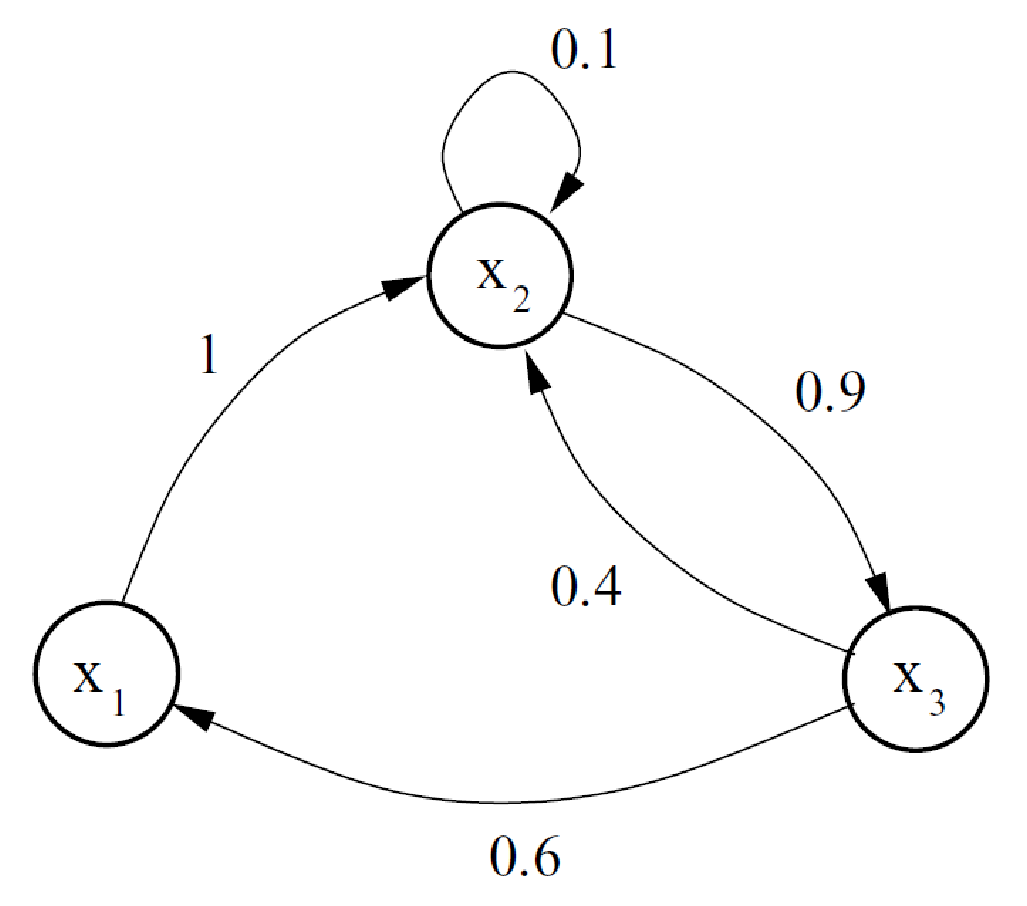
\includegraphics[width=0.5\linewidth]{sampMarkovTransitionGraph}
\caption{Transition graph for Markov chain example. }
\label{fig:sampMarkovTransitionGraph}
\end{figure}

\begin{equation}
\label{equ:sampMarkovNextTimeProbability}
\begin{aligned}
{u^{*1}}_j &= \sum\limits_{i = 0}^2 {{u^{*0}}_ip\left( {{x^{*1}} = j|{x^{*0}} = i} \right)}  = \sum\limits_{i = 0}^2 {{u^{*0}}_i{m_{ij}}} \\
 \Rightarrow {u^{*1}} &= {u^{*0}}m
\end{aligned}
\end{equation}
After several iterations (multiplication by $m$), the product $u^{*t}$ converges to $\left(0.2, 0.4, 0.4\right)$. 
In fact, no matter what initial distribution we use, the chain will stabilize at $\left(0.2, 0.4, 0.4\right)$. This stability result plays a fundamental role in sampling.
We here give the theorem of the convergence of the Markov chain as The.\ref{the:sampConvergenceOfMarkovChain}.

\begin{theorem}[Convergence of Markov chain]
\label{the:sampConvergenceOfMarkovChain}
For both discrete and continuous variable, from any probability distribution, the Markov chain (result of multiplications by $m$) will convergence to invariant distribution $\pi \left(x\right)$, as long as $m$ is a \emph{stochastic} transition matrix that obeys the following properties:

\begin{itemize}
\item [1.] \textbf{Irreducibility}. For any state of the Markov chain, there is a positive probability of visiting all other states (direct or indirect connection). That is, the matrix $m$ can not be reduced to separate smaller matrices, which is also the same as stating that the transition graph is connected (one state can reach any other state through the transition graph).
\item[2.] \textbf{Aperiodicity}. For one state, the times of the result of transition back to itself is always the integral multiple of $a$, we consider such Markov chain has periodicity. The chain should not be periodic (get trapped in cycles). 
\end{itemize}
\end{theorem}

\textbf{A sufficient, but not necessary, condition to ensure that one Markov chain will convergence to invariant distribution is that there are the direct or indirect connections between all the pairs of two states (the PageRank algorithm make sure any two nodes have connection by add a damping factor). 
***Here is only my assumption.}

A sufficient, but not necessary, condition to ensure that one particular $\pi \left(x\right)$ is the desired invariant distribution is the following reversibility (detailed balance) condition as described in Eq.~\ref{equ:sampMarkovDetailedBalanceDerivation}.

\begin{equation}
\label{equ:sampMarkovDetailedBalanceDerivation}
\begin{aligned}
\pi \left( j \right){m_{ji}} &= \pi \left( i \right){m_{ij}}\\
 \Rightarrow \tilde \pi \left( i \right) &= {\left( {\pi m} \right)_i} = \sum\limits_j {\pi \left( j \right){m_{ji}}} \\
 &= \sum\limits_j {\pi \left( i \right){m_{ij}}} \\
 &= \pi \left( i \right)\sum\limits_j {{m_{ij}}} \\
 &= \pi \left( i \right)
\end{aligned}
\end{equation}

Let $r$ denotes a distribution, $m$ denotes the transition probability matrix, ${\tilde r}$ denotes the translated distribution by multiplying $m$. Then we have 
 
\begin{equation}
\label{equ:translated_distribution}
\tilde r\left( i \right) = \sum\limits_j {r\left( j \right){m_{ji}}}
\end{equation}

If we drawn $n$ data from $r$, we have 

\begin{equation}
\label{equ:markov_proof_drawn_data_probability}
\begin{aligned}
|{S_i}| &= nr\left( i \right)\\
|{{\tilde S}_i}| &= \sum\limits_j {nr\left( j \right){m_{ji}}} \\
 &= n\sum\limits_j {r\left( j \right){m_{ji}}} \\
 &= n\tilde r\left( i \right)
\end{aligned}
\end{equation}
where $|{S_i}|$ is the size of data at value $i$ under the distribution $r$, $|{{\tilde S}_i}|$ is the size of data at value $i$ after transition. We can see that $|{{\tilde S}_i}|$ is the size of data at value $i$ under the distribution $\tilde r$.
Hence we drawn data from $r$, after applying transition according the transition probability matrix $m$, the translated data can be considered the drawn data from $r \times m$.

Markov Chain can be used for drawning data from a arbitrarily distribution. 
Specifically, if we want to sample $n$ data from distribution $\pi$, we first random generate $n$ initial data (they even can be all the same).
Then we design a transition probability matrix $m$ that satisfies the convergence conditions of irreducibility and aperiodicity, and the detailed balance condition defined in Eq.~\ref{equ:sampMarkovDetailedBalanceDerivation}.
According the transition probability matrix, we modify each drawn data.
After perform sufficient steps of modification, the final data can be condidered the drawn data from distribution $\pi$.
We will discribe drawn details in Sec.\ref{sec:metropolis_hastings_sampling}.




\section{Sampling}
Sampling has two types: sampling from a distribution or sampling from a population. For sampling from a distribution, we need to sample data from the distribution, in other word, the sampled data should satisfy the probability distribution. For sampling from a population, we need to sample data from the population, that is to say, we select the part of the data of the population. In this section, we will discuss the sampling algorithm in the two types of sampling.

\subsection{Discrete Variable and Continuous Variable}
As we know, probability distribution is for both discrete distribution and continuous distribution. However, the PMF is only for discrete distribution and PDF is only for continuous distribution. For simplifying processing in some math derivation, we introduce the conversion between discrete distribution and continuous distribution.

For the conversion from discrete distribution to continuous distribution, we consider the discrete variable $x$ as the continuous variable in $\tilde x \in \left[x, x + 1\right)$. Thus the discrete variable can be considered as the uniform distribution in each $\left[x, x + 1\right)$ (note that the $p\left(\tilde{x}\right) = p\left(x\right)$). 
For the conversion from continuous distribution to discrete distribution, we select a unit range $dx$ and consider the range $\left[x, x + dx\right)$ as a discrete variable $\tilde{x}$. Then we have $p\left(\tilde{x}\right) = \int\limits_x^{x + dx} {p\left( a \right)da} $. 
Notice that conversion from discrete distribution to continuous distribution is lossless (as shown in Fig.\ref{fig:sampPMFConverted}) while the other is lossless (as shown in Fig.\ref{fig:sampPDFConverted}).

\begin{figure}
\centering
\subfigure[Source PMF]{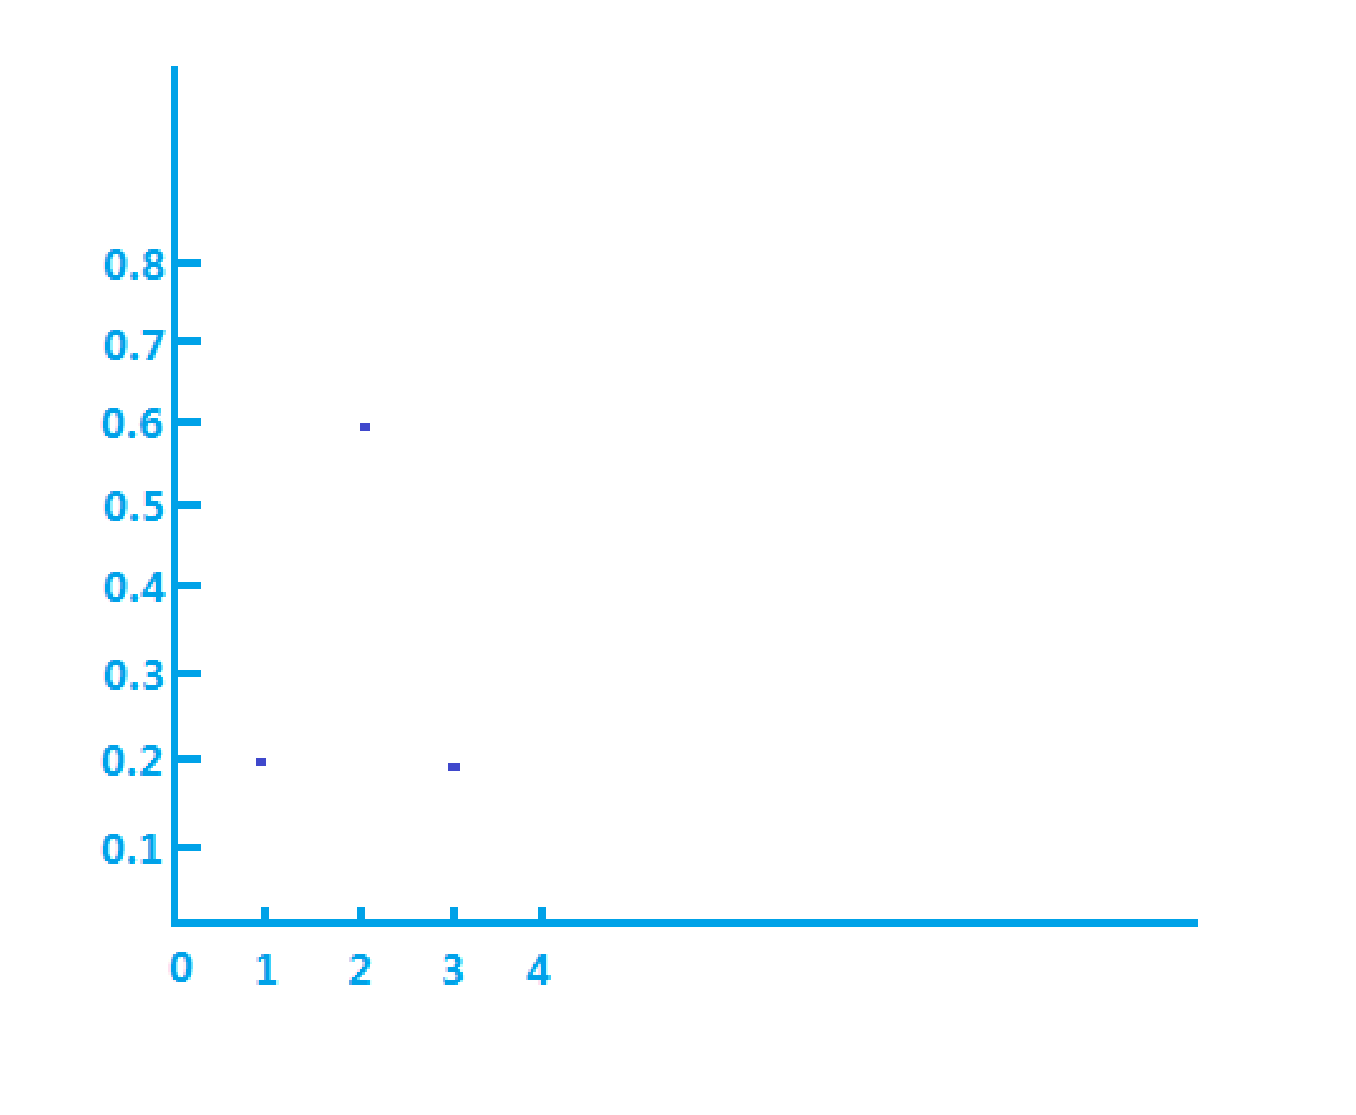
\includegraphics[width=0.48\linewidth]{sampleExamplePMFSource}}
\subfigure[PDF converted from PMF]{\includegraphics[width=0.48\linewidth]{sampleExamplePMFToPDF}}
\caption{Illustration of the PMF and the PDF converted from corresponding PMF. We can recovered the original PMF from the PDF.}
\label{fig:sampPMFConverted}
\end{figure}

\begin{figure}
\centering
\subfigure[Source PDF]{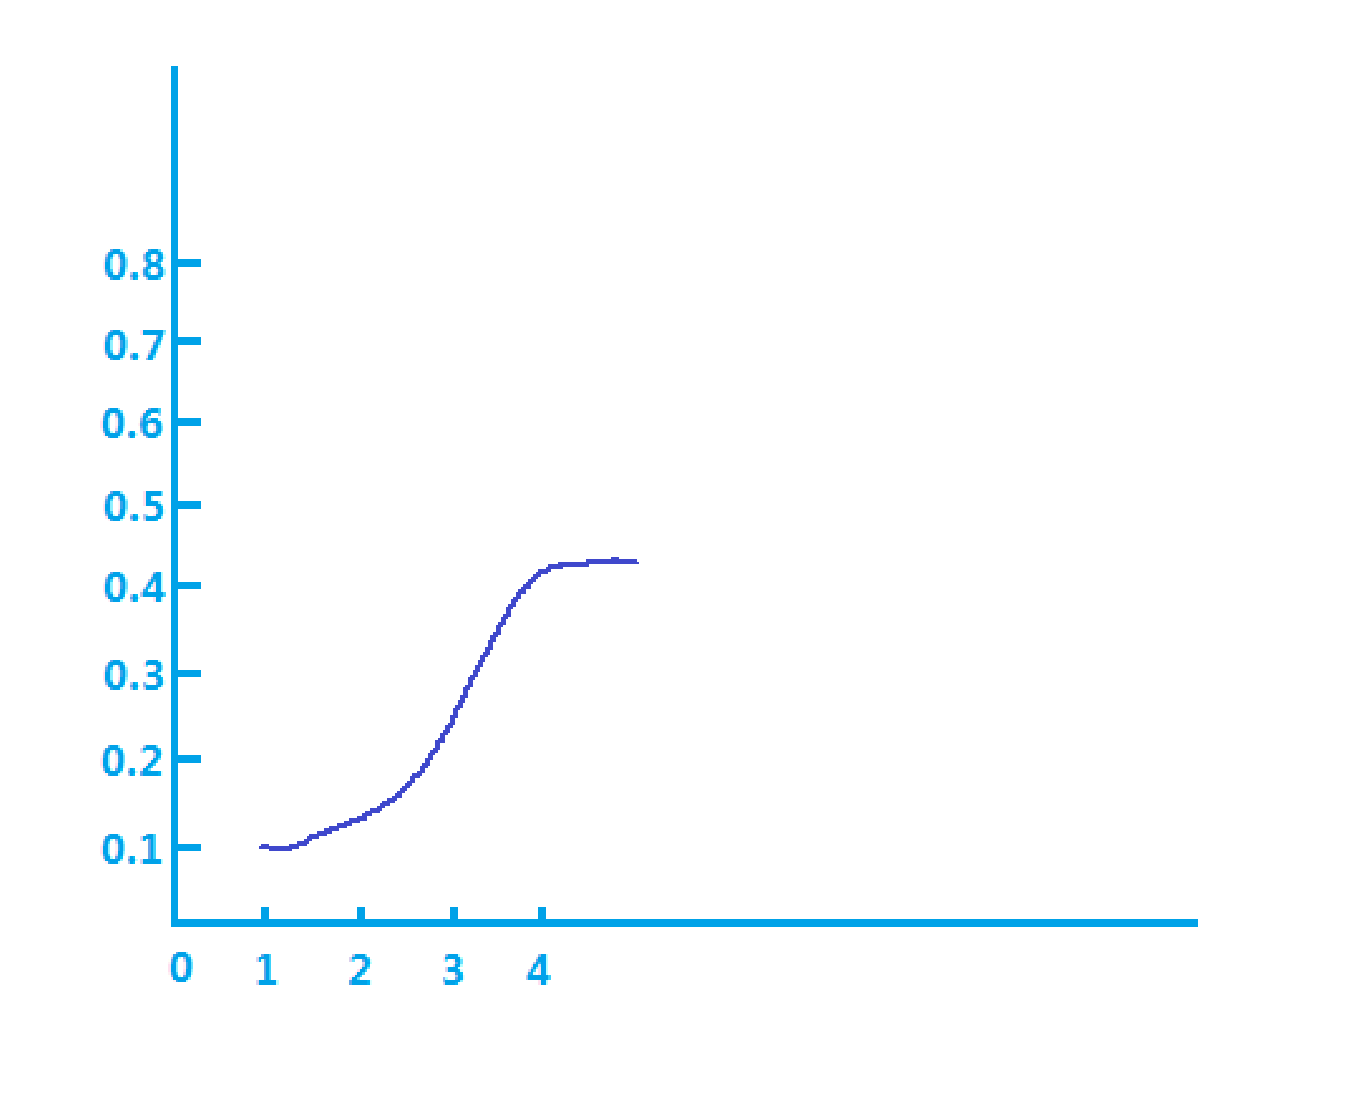
\includegraphics[width=0.48\linewidth]{sampleExamplePDFSource}}
\subfigure[PMF converted from PDF]{\includegraphics[width=0.48\linewidth]{sampleExamplePDFToPMF}}
\subfigure[PDF recovered by PMF]{\includegraphics[width=0.48\linewidth]{sampleExampleRecoverPDF}}
\caption{Illustration of the PDF, the PMF converted from corresponding PDF and the recovered PDF by PMF. Notice that if we select more discrete variable, the recovered PDF will be more closed to the source PDF.}
\label{fig:sampPDFConverted}
\end{figure}

\subsection{Sampling From a Distribution}
The object of sampling from a distribution can be formalized by Eq.~\ref{equ:sampDistributionObject}.

\begin{equation}
\label{equ:sampDistributionObject}
\forall a,\tilde F\left( a \right) = P\left( {x \le a;\tilde F} \right) \approx F\left( a \right) = P\left( {x \le a;F} \right)
\end{equation}
Where $F$ denotes the probability distribution function, $P$ denotes the probability for event. $\tilde F$ and $\tilde{p}$ are for the probability distribution function and probability function in sampled data. 

From the aspect of PDF (the discrete distribution will be convert to continuous variable for simple discussion), the sample points in each range $\left(x, x + dx\right)$ of variable should be positive proportional to the probability in the range ($p\left(x\right)dx$ for continuous variable or $p\left(x\right)$). If we let the sampled points in range to disperse symmetrically for the range (note that the $x$ is the same in a unit range $dx$), then the sampling process is just like to sampled points (each point contains the properties and probability density) from the area under the curve of probability function, as shown in Fig.\ref{fig:sampProbabilityFunction}.

\begin{figure}
\centering
\subfigure[]{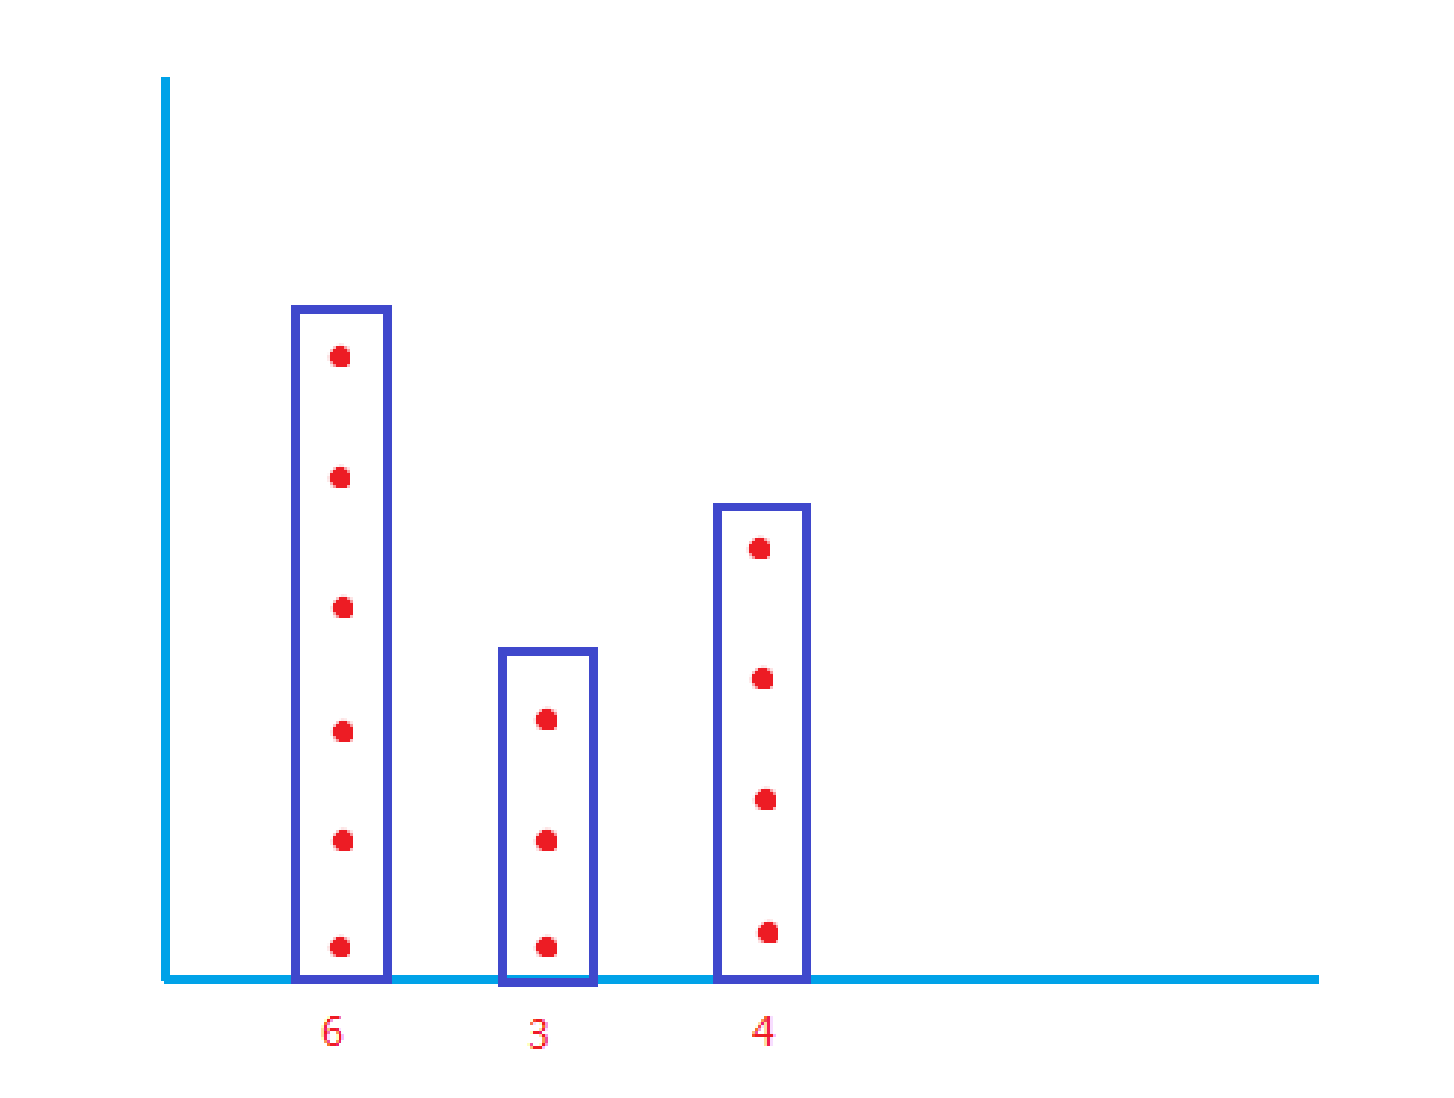
\includegraphics[width=0.48\linewidth]{sampFromPMF}}
\subfigure[]{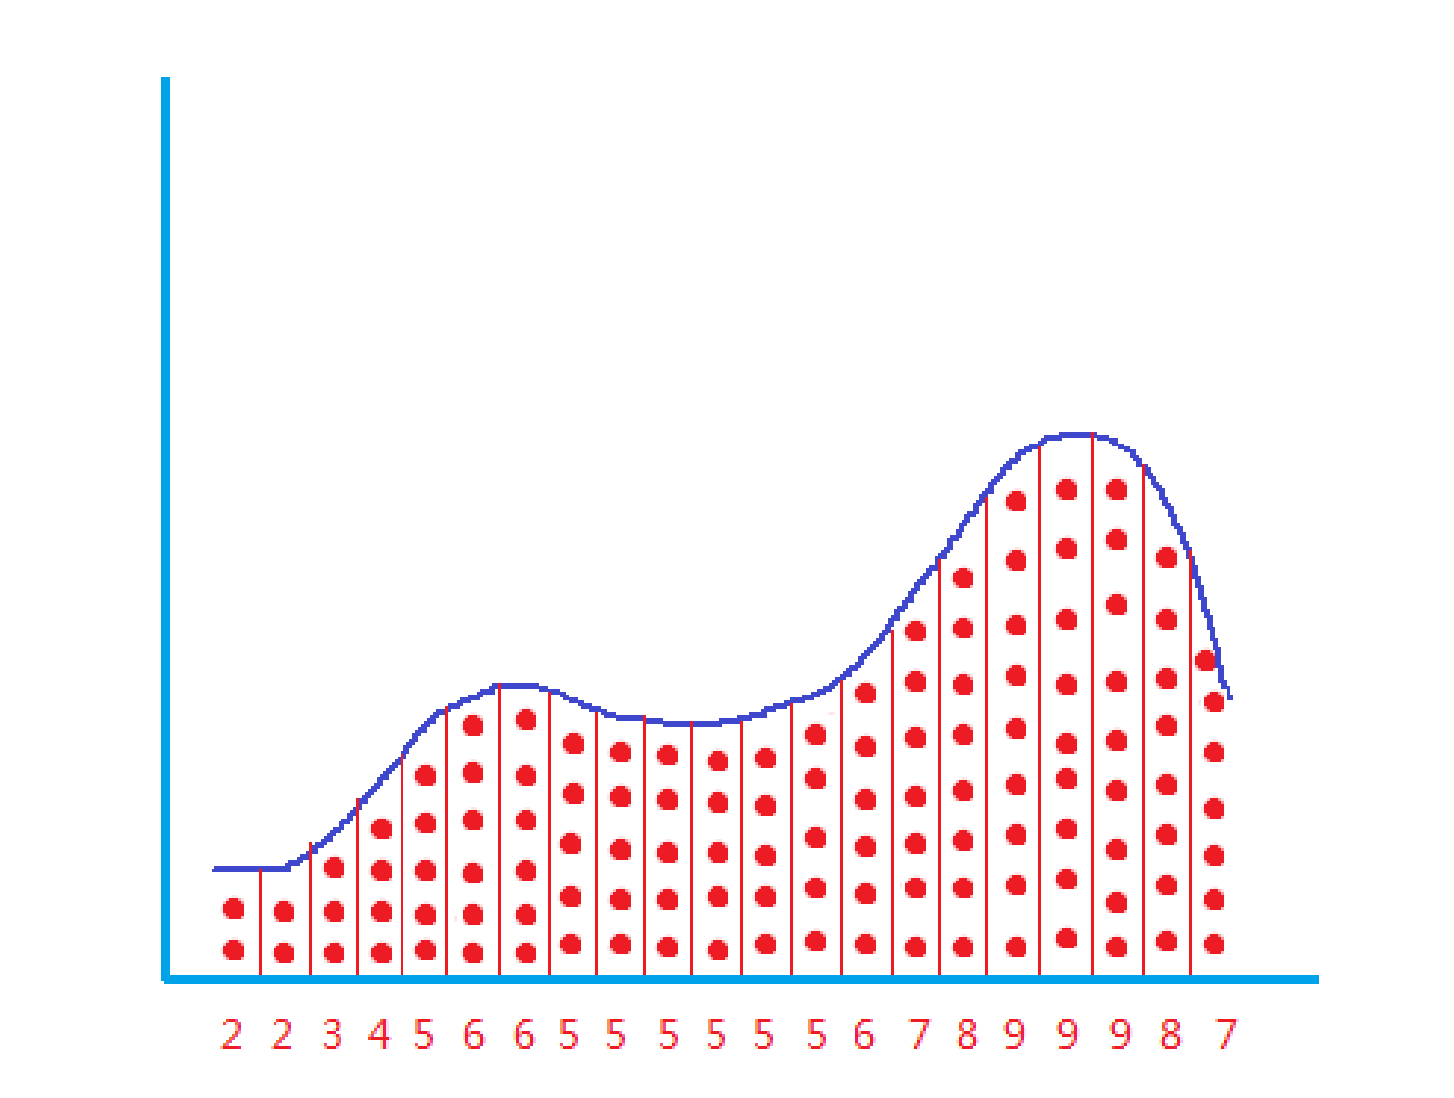
\includegraphics[width=0.48\linewidth]{sampFromPDF}}
\caption{Illustration of the sampling process in discrete variable and continuous variable in the aspect of probability function. The red points are the sampled points. Note that we consider the discrete variable as continuous variable.}
\label{fig:sampProbabilityFunction}
\end{figure}

In the following subsections, we will discuss the \emph{specified sampling} methods (direct sampling, accepting-rejecting sampling, replacement sampling) and \emph{uniform sampling} methods (Markov Chain sampling).

\subsection{Direct Sampling Method}
We can use Eq.~\ref{equ:sampDirectSamplingBias} to sample data from any distributions.

\begin{equation}
\label{equ:sampDirectSamplingBias}
{x^i} = {F^{ - 1}}\left( {{\varepsilon ^i}} \right),i = 0,1,...n - 1
\end{equation}
Where $x^{*i}$ is the $ith$ data sampled from distribution $F$. $\varepsilon ^{*i}$ is the $ith$ random value whose range is in $\left[0, 1\right]$.

We can prove the data sampled fully and independently from distribution $F$ approximately satisfy $F$, as shown in Eq.~\ref{equ:sampProve}.
\begin{equation}
\label{equ:sampProve}
\begin{aligned}
\tilde F\left( {\tilde a} \right) &= P\left( {x \le \tilde a; \tilde{F}} \right)\\
 &= P\left( {x = {F^{ - 1}}\left( \varepsilon  \right) \le \tilde a} \right)\\
 &= P\left( {\varepsilon  \le F\left( {\tilde a} \right)} \right)\\
 &= p\left( {x \le \tilde a; F} \right)\\
 &= F\left( {\tilde a} \right)
\end{aligned}
\end{equation}
Where $P$ denotes the probability of the event in this sampling process, $\tilde{F}$ denotes the probability distribution function that sampled data satisfy.

For discrete distributions, we have the more exact sampling rule as shown in Eq.~\ref{equ:sampDiscrete}.

\begin{equation}
\label{equ:sampDiscrete}
{x^{*i}} = {x^{*k}},\sum\limits_{j = 0}^{k - 1} {p\left( {{x^{*j}}} \right)}  < {\varepsilon ^{*i}} \le \sum\limits_{j = 0}^k {p\left( {{x^{*j}}} \right)}
\end{equation} 
Where $x^{*k}$ is the $kth$ discrete discrete jumping point.

For a continuous distribution, if the probability distribution function has inverse function, then the sampling method can be described by Eq.~\ref{equ:sampContinuous}.

\begin{equation}
\label{equ:sampContinuous}
{x^{*i}} = {F^{ - 1}}\left( {{\varepsilon ^{*i}}} \right)
\end{equation}

However, the inverse function is not always existent or simple to compute. So we introduce the following sampling methods to deal with such distributions.

\subsection{Accepting-Rejecting Sampling}
\label{sec:sampAcceptingRejecting}
It is difficult to sample data from a distribution $p$ when its inverse function is not existent or complicated to compute. However, we can adopt a indirect method to sample data. 

Since the sampling process can be considered sample points symmetrically in the area under probability function (here is the PDF), so we can first sample points from $mh$ where h is a simple distribution and the curve of $mh$ is above the $p$ ($m$ is the scale ratio to make sure the curve $mh$ is above $p$ in any point, $m \ge 1$). 
Then the points (include properties and probability) under the curve of $p$ can be considered the symmetrical sampling result from $p$. 
So in each $dx$, we first sample $nmh\left(x\right)dx$ data, then we random select $np\left(x\right)dx$ data, as shown in Fig.~\ref{fig:sampAcceptingRejecting}. The mathematical proof is described in Eq.~\ref{equ:sampAcceptingRejectingProof}. Obviously, if we want to sample $n$ data from distribution $p$, then we need to sample $nm$ data from distribution $h$. Thus the sampling efficiency is $\frac{1}{m}$ that can be proved by Eq.~\ref{equ:sampAcceptionExpectation}.

\begin{equation}
\label{equ:sampAcceptionExpectation}
\begin{aligned}
P\left( {x\ accepted} \right) &= E\left( {\frac{{p\left( x \right)}}{{mq\left( x \right)}}} \right)\\
 &= \int\limits_{ - \infty }^{ + \infty } {\frac{{p\left( x \right)}}{{mq\left( x \right)}}q\left( x \right)dx} \\
 &= \frac{1}{m}\int\limits_{ - \infty }^{ + \infty } {p\left( x \right)dx} \\
 &= \frac{1}{m}
\end{aligned}
\end{equation}

\begin{equation}
\label{equ:sampAcceptingRejectingProof}
\begin{aligned}
\tilde p\left( x \right)dx &= P\left( {x < \tilde x < x + dx; \tilde{p}} \right)\\
 &= P\left( {x < \hat x < x + dx|\varepsilon  \le \frac{{p\left( {\hat x} \right)}}{{mh\left( x \right)}}} \right)\\
 &= \frac{{P\left( {x < \hat x < x + dx,\varepsilon  \le \frac{{p\left( {\hat x} \right)}}{{mh\left( x \right)}}} \right)}}{{P\left( {\varepsilon  \le \frac{{p\left( {\hat x} \right)}}{{mh\left( x \right)}}} \right)}}\\
 &= \frac{{\int_x^{x + dx} {\int_0^{\frac{{p\left( {\hat x} \right)}}{{mh\left( x \right)}}} {h\left( {\hat x} \right)d\hat x \cdot d\varepsilon } } }}{{\int_{ - \infty }^\infty  {\int_0^{\frac{{p\left( {\hat x} \right)}}{{mh\left( x \right)}}} {h\left( {\hat x} \right)d\hat x \cdot d\varepsilon } } }}\\
 &= \frac{{\int_x^{x + dx} {h\left( {\hat x} \right)\frac{{p\left( {\hat x} \right)}}{{mh\left( x \right)}}d\hat x} }}{{\int_{ - \infty }^\infty  {h\left( {\hat x} \right)\frac{{p\left( {\hat x} \right)}}{{mh\left( x \right)}}d\hat x} }}\\
 &= \frac{{\int_x^{x + dx} {p\left( {\hat x} \right)d\hat x} }}{{\int_{ - \infty }^\infty  {p\left( {\hat x} \right)d\hat x} }}\\
 &= \int_x^{x + dx} {p\left( {\hat x} \right)d\hat x} \\
 &= p\left( x \right)dx
\end{aligned}
\end{equation}
Where $\tilde{p}$ denote the PDF that the sampled data satisfy. ${\tilde x}$ and ${\hat x}$ denote the variable in $\tilde{p}$ and $h$ respectively.

\begin{figure}
\centering
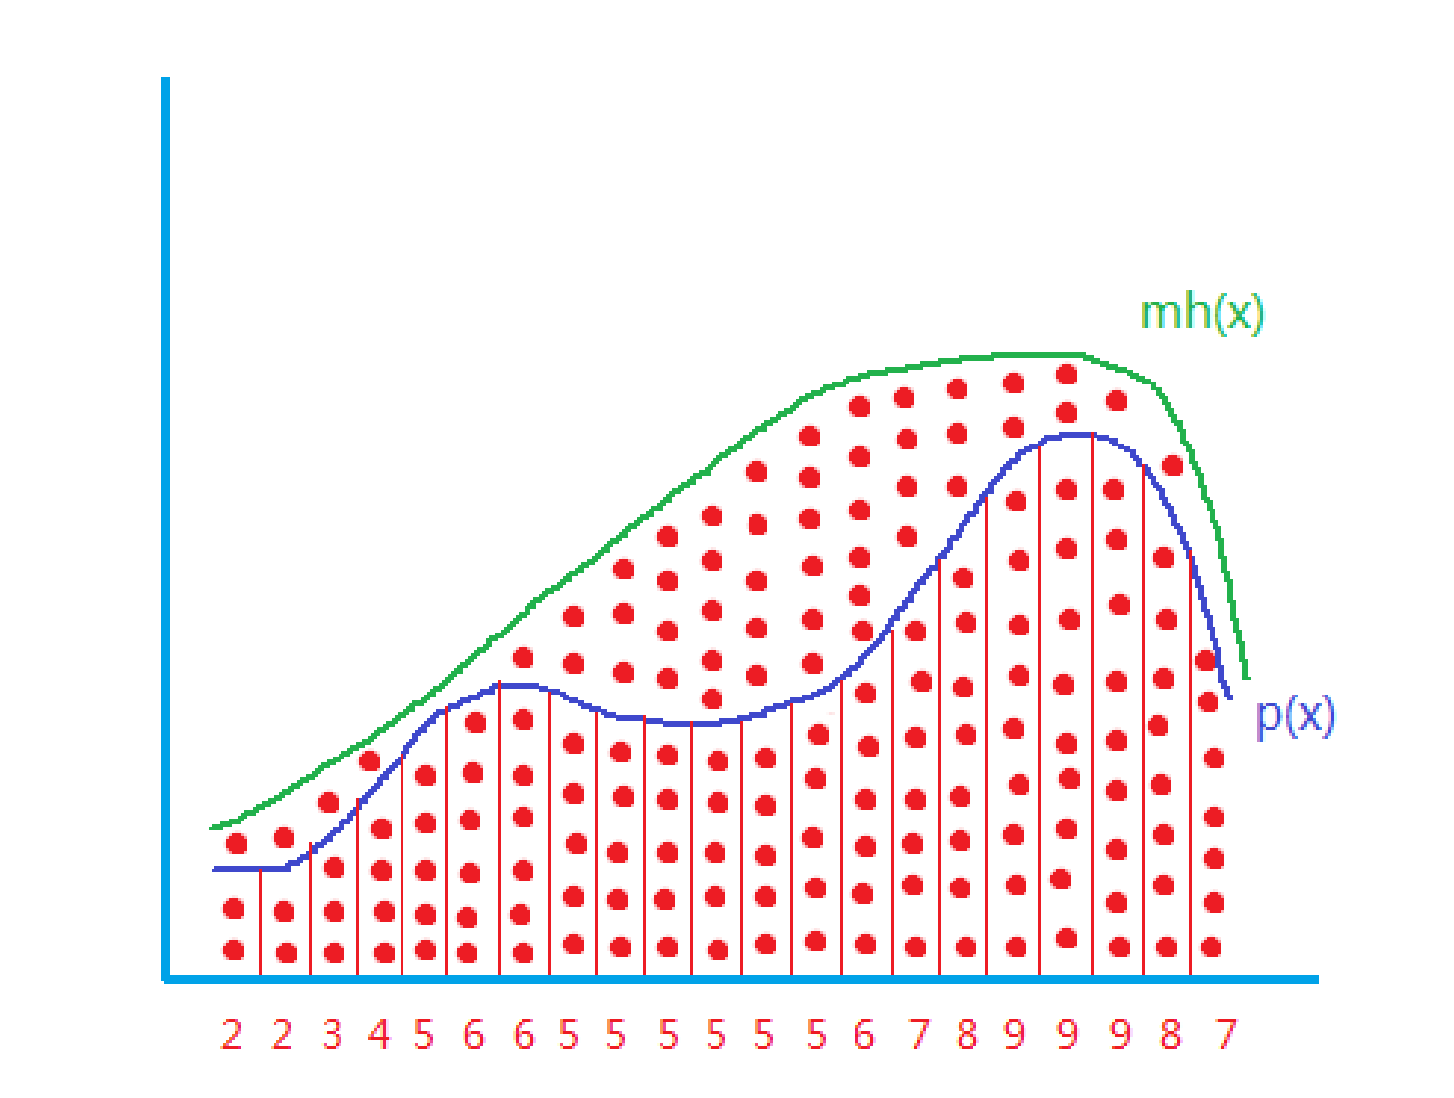
\includegraphics[width=0.7\linewidth]{sampAcceptingRejecting}
\caption{Illustration of the accepting-rejecting sampling. The data sampled from $mh\left(x\right)$ are symmetrical in the area under $p\left(x\right)$. }
\label{fig:sampAcceptingRejecting}
\end{figure}

In order to get high sampling efficiency (if we want to sample $n$ data from $p$, we need sample $nm$ data from $h$), we need to find a small $m$ and a small $m$ means $h$ is similar to $p$. The sampling process can be described as flowing:

\begin{itemize}
  \item Find a distribution $h$ and $m$,
  \item Sample a data $x$ from distribution $h$,
  \item Get a random value $\varepsilon$ in $\left[0, 1\right]$,
  \item if $\varepsilon \le {\frac{{p\left( {x} \right)}}{{mh\left( x \right)}}} $, we consider it as a valid data for $p$.
\end{itemize}

\subsection{Replacement Sampling}
For some sampling of distributions with very complicated form of variables but can be simplified by some middle variables, we can adopt the replacement sampling. We give a example for sampling from the Gaussian distribution.

For a 1-d normal Gaussian distribution, its probability density function can be formalized by Eq.~\ref{equ:sampNormalGaussianPDF}.

\begin{equation}
\label{equ:sampNormalGaussianPDF}
p\left( x \right) = \frac{1}{{\sqrt {2\pi } }}\exp \left( { - \frac{{{x^2}}}{2}} \right)
\end{equation}

We introduce a variable $y$ which is independent with $x$ and satisfies the same distribution with $x$. Then the joint probability distributions can be formalized by Eq.~\ref{equ:sampNormalGaussianJointPDF}.

\begin{equation}
\label{equ:sampNormalGaussianJointPDF}
p\left( {x,y} \right) = \frac{1}{{2\pi }}\exp \left( { - \frac{{{x^2} + {y^2}}}{2}} \right)
\end{equation}

Then we introduce two middle variables $\rho$ and $\varphi$ that satisfy the following Eq.~\ref{equ:sampNormalReplaceVariables}.

\begin{equation}
\label{equ:sampNormalReplaceVariables}
\begin{aligned}
x &= \rho \cos \varphi \\
y &= \rho \sin \varphi \\
s.t.&\ \rho  > 0,\ \varphi  \in \left[ {0,2\pi } \right]
\end{aligned}
\end{equation}

Eq.~\ref{equ:sampNormalGaussianJointPDF} can be converted to Eq.~\ref{equ:sampNormalGaussianMiddleVariables}.

\begin{equation}
\label{equ:sampNormalGaussianMiddleVariables}
\begin{aligned}
p\left( {\rho ,\varphi } \right) &= \frac{{{d^2}F\left( {\rho ,\varphi } \right)}}{{d\rho d\varphi }}\\
 &= \frac{{{d^2}F\left( {x\left( {\rho ,\varphi } \right),y\left( {\rho ,\varphi } \right)} \right)}}{{dxdy}}|\frac{{d\left( {x,y} \right)}}{{d\left( {\rho ,\varphi } \right)}}|\\
 &= p\left( {x,y} \right)|\frac{{d\left( {x,y} \right)}}{{d\left( {\rho ,\varphi } \right)}}|\\
 &= \frac{1}{{2\pi }}\exp \left( { - \frac{{{x^2} + {y^2}}}{2}} \right)|\begin{array}{*{20}{c}}
{\frac{{\partial x}}{{\partial \rho }}}&{\frac{{\partial x}}{{\partial \varphi }}}\\
{\frac{{\partial y}}{{\partial \rho }}}&{\frac{{\partial y}}{{\partial \varphi }}}
\end{array}|\\
 &= \frac{1}{{2\pi }}\exp \left( { - \frac{{{\rho ^2}}}{2}} \right)|\begin{array}{*{20}{c}}
{\cos \varphi }&{ - \rho \sin \varphi }\\
{\sin \varphi }&{\rho \cos \varphi }
\end{array}|\\
 &= \frac{\rho }{{2\pi }}\exp \left( { - \frac{{{\rho ^2}}}{2}} \right)
\end{aligned}
\end{equation}

From Eq.~\ref{equ:sampNormalGaussianMiddleVariables}, we can further know that the margin PDF for $\rho$ and $\varphi$ due to the integral of margin PDF should be 1, as shown in Eq.~\ref{equ:sampNormalMiddleVariableMarginPDFs}.

\begin{equation}
\label{equ:sampNormalMiddleVariableMarginPDFs}
\begin{aligned}
p\left( \rho  \right) &= \rho \exp \left( { - \frac{{{\rho ^2}}}{2}} \right),\ \rho  > 0\\
p\left( \varphi  \right) &= \frac{1}{{2\pi }},\ \varphi  \in \left[ {0,2\pi } \right]
\end{aligned}
\end{equation}

The probability distribution function and inverse function can be computed directly, as shown in Eq.~\ref{equ:sampNormalMiddleVariableMarginProbabilityDistributionFunction}.

\begin{equation}
\label{equ:sampNormalMiddleVariableMarginProbabilityDistributionFunction}
\begin{aligned}
F\left( \rho  \right) &=  - \exp \left( { - \frac{{{\rho ^2}}}{2}} \right),\ \varphi  \in \left[ {0,2\pi } \right]\\
F\left( \varphi  \right) &= \frac{\varphi }{{2\pi }},\ \varphi  \in \left[ {0,2\pi } \right]\\
\rho &= {F^{ - 1}}\left( \varepsilon  \right) = \sqrt { - 2\ln \left( { 1 - \varepsilon } \right)} ,\ \varepsilon  \in \left[ {0,1} \right]\\
\varphi &= {F^{ - 1}}\left( \varepsilon  \right) = 2\pi \varepsilon ,\ \varepsilon  \in \left[ {0,1} \right]
\end{aligned}
\end{equation}

Then we can adopt the direct sampling method to sample $\rho$ and $\varphi$, the data satisfy normal Gaussian distribution can get by the Eq.~\ref{equ:sampDataOfNormalGaussian}.

\begin{equation}
\label{equ:sampDataOfNormalGaussian}
\begin{aligned}
{x^{*2i}} &= \sqrt { - 2\ln \left( { 1 - {{\tilde \varepsilon }^{*i}}} \right)} \cos 2\pi {{\hat \varepsilon }^{*i}}\\
{x^{*2i + 1}} &= \sqrt { - 2\ln \left( { 1 - {{\tilde \varepsilon }^{*i}}} \right)} \sin 2\pi {{\hat \varepsilon }^{*i}}
\end{aligned}
\end{equation}
Where we sample one time by random two value $\tilde \varepsilon$ and $\hat \varepsilon$ to generate two data.

The sampling from non-normal Gaussian distribution can be extended by the normal Gaussian distribution, as shown in Eq.~\ref{equ:sampDataOfNonNormalGaussian}.

\begin{equation}
\label{equ:sampDataOfNonNormalGaussian}
{{\tilde x}^{*i}} = x^{*i}\sigma  + u
\end{equation}

Now we discuss the sampling from multivariate Gaussian distribution. We first discuss the distribution with zero average value. The PDF is shown as Eq.~\ref{equ:sampMultiGaussianZeroAvarage}.

\begin{equation}
\label{equ:sampMultiGaussianZeroAvarage}
p\left( x \right) = {\left( {2\pi } \right)^{ - \frac{d}{2}}}| \Sigma |^{-\frac{1}{2}}\exp \left\{ { - \frac{1}{2}{x} {\Sigma ^{ - 1}}{{{x}}^t}} \right\}
\end{equation}

Because the existence of covariance, the different dimensions have relativities so that we can not sample independently in each dimension. However, inspired by the matrix similarity (the covariance matrix is real symmetric matrix and can be similar to a diagonal matrix), we can convert the Eq.~\ref{equ:sampMultiGaussianZeroAvarage} as Eq.~\ref{equ:sampMultiGaussianDiagonal} shows.

\begin{equation}
\label{equ:sampMultiGaussianDiagonal}
\begin{aligned}
p\left( x \right) &= {\left( {2\pi } \right)^{ - \frac{d}{2}}}| \Sigma |^{-\frac{1}{2}}\exp \left\{ { - \frac{1}{2}x{\Sigma ^{ - 1}}{x^t}} \right\}\\
 &= {\left( {2\pi } \right)^{ - \frac{d}{2}}}| \Sigma |^{-\frac{1}{2}}\exp \left\{ { - \frac{1}{2}x{{\left( {{Q^t} \wedge Q} \right)}^{ - 1}}{x^t}} \right\}\\
 &= {\left( {2\pi } \right)^{ - \frac{d}{2}}}| \Sigma |^{-\frac{1}{2}}\exp \left\{ { - \frac{1}{2}xQ \wedge {Q^t}{x^t}} \right\}\\
 &= {\left( {2\pi } \right)^{ - \frac{d}{2}}}| \wedge |^{-\frac{1}{2}}\exp \left\{ { - \frac{1}{2}xQ \wedge {{\left( {xQ} \right)}^t}} \right\}
\end{aligned}
\end{equation}
Where $Q$ is the matrix combined the eigenvectors (vertical) and $\wedge$ is the diagonal matrix consisted of eigenvalues. Note that $Q^t = Q^{-1}$.

Let $\hat{x}$ denotes $xQ$, then $\hat{x}$ satisfy the distribution as shown in Eq.~\ref{equ:sampMultiGaussianIndependent}.

\begin{equation}
\label{equ:sampMultiGaussianIndependent}
p\left( {\hat x} \right) = {\left( {2\pi } \right)^{ - \frac{d}{2}}}| \wedge |^{-\frac{1}{2}}\exp \left\{ { - \frac{1}{2}\hat x \wedge {{\hat x}^t}} \right\}
\end{equation}
Where $p\left(\hat{x}\right)$ is independent for each dimension so that we can sample the data easily. Specifically, suppose that we want sample $n \times m$ data where $n$ denotes the count of data and $m$ denotes the dimension of data. We first sample $n \times 1$ data satisfied normal Gaussian distribution. Then the data will be multiplied by d variances (the eigenvalues of matrix $Q$) to get $n \times m$ data.
Then $x$ can be gotten by Eq.~\ref{equ:sampDataOfZeroMultiGaussian}.

\begin{equation}
\label{equ:sampDataOfZeroMultiGaussian}
x^{*i} = \hat{x}^{*i}Q^{t}
\end{equation}

For the multivariate distribution with non-zero average value, its PDF is shown in Eq.~\ref{equ:sampMultiGaussianNoZero}.

\begin{equation}
\label{equ:sampMultiGaussianNoZero}
p\left(\tilde{x} \right) = {\left( {2\pi } \right)^{ - \frac{d}{2}}}| \Sigma |^{-\frac{1}{2}}\exp \left\{ { - \frac{1}{2}\left( {\tilde x - u} \right){\Sigma ^{ - 1}}{{\left( {\tilde x - u} \right)}^t}} \right\}
\end{equation}

Let $x$ denotes $\tilde x - u$, then we can first sample data $x$ from the corresponding distribution with zero average value, the add the average value $u$ for each sampled data to get $\tilde x$, as shown in Eq.~\ref{equ:sampDataOfNonZeroMultiGaussian}.

\begin{equation}
\label{equ:sampDataOfNonZeroMultiGaussian}
\tilde x^{*i} = x^{*i} + u
\end{equation}

\subsection{Metropolis-Hastings Sampling}
\label{sec:metropolis_hastings_sampling}
As descried in Sec.~\ref{sec:sampMarkovChain}, if we want to drawn data from distribution $\pi$, we can first random generate $n$ initial data.
Then we design a transition probability matrix $m$ that satisfies the convergence conditions of irreducibility and aperiodicity, and the detailed balance condition defined.
According the transition probability matrix, we modify each drawn data.
After perform sufficient steps of modification, the final data can be condidered the drawn data from distribution $\pi$.
Hence the key factor is the transition probability matrix.

Since the transition probability matrix decide the final convergence probability distribution (the distribution we want to drawn data from), the transition probability matrix must contains the information of final convergence distribution.
We observe the detailed balance condition defined as

\begin{displaymath}
\label{equ:metropolis_hastings_sampling_detailed_balance}
\pi \left( j \right){m_{ji}} = \pi \left( i \right){m_{ij}}
\end{displaymath}
then we have 

\begin{displaymath}
{m_{ij}} = \frac{{\pi \left( j \right){m_{ji}}}}{{\pi \left( i \right)}}
\end{displaymath}
however, this is a recursive representation, we use a intermediate probability transition matrix $q$ to replace the $m$, then we have

\begin{displaymath}
{m_{ij}} = \frac{{\pi \left( j \right){q_{ji}}}}{{\pi \left( i \right)}}
\end{displaymath}
however, $m\left[ {i,j} \right]$ may exceed $1$ that is invalid probability value, 
basides, to make sure $\sum\limits_j {{m_{ij}}}  = 1$, we add the restrict term as follows

\begin{displaymath}
{m_{ij}} = \min \left\{ {\frac{{\pi \left( j \right){q_{ji}}}}{{\pi \left( i \right)}},{q_{ij}}} \right\}
\end{displaymath}

Here we verify the detailed balance condition under the designed probability transition matrix.

\begin{displaymath}
\label{equ:metropolis_hastings_sampling_detailed_balance_proof}
\begin{aligned}
\pi \left( i \right){m_{ij}} &= \pi \left( i \right)\min \left\{ {\frac{{\pi \left( j \right){q_{ji}}}}{{\pi \left( i \right)}},{q_{ij}}} \right\}\\
 &= \min \left\{ {\pi \left( j \right){q_{ji}},\pi \left( i \right){q_{ij}},} \right\}\\
 &= \pi \left( j \right)\min \left\{ {{q_{ji}},\frac{{\pi \left( i \right){q_{ij}}}}{{\pi \left( j \right)}}} \right\}\\
 &= \pi \left( j \right)\min \left\{ {\frac{{\pi \left( i \right){q_{ij}}}}{{\pi \left( j \right)}},{q_{ji}}} \right\}\\
 &= \pi \left( j \right){m_{ji}}
\end{aligned}
\end{displaymath}

Now the only question is how to get the variable value in next step for a given variable value. In fact, for a given state $i$ of variable $x$, the next variable $j$ satisfy the probability distribution defined by $p\left( {x = j} \right) = {m_{ij}}$. Hence to get the next variable value can be taken as drawn a sample from distribution $p\left( {x = j} \right) = {m_{ij}}$. 
We modify the $m_{ij}$ to 

\begin{displaymath}
\label{equ:metropolis_hastings_sampling_acept_rejecting}
\begin{aligned}
{m_{ij}} &= \min \left\{ {\frac{{\pi \left( j \right){q_{ji}}}}{{\pi \left( i \right)}},{q_{ij}}} \right\}\\
 &= \min \left\{ {\frac{{\pi \left( j \right){q_{ji}}}}{{\pi {{\left( i \right)}_{ij}}}},1} \right\}{q_{ij}}
\end{aligned}
\end{displaymath}

We can adopt the accepting-rejecting drawning to drawn a the $j$. 
Specifically, we first drawn data from $p\left( {x = j} \right) = {q_{ij}}$, then we accept the drawn result in a probability $\min \left\{ {\frac{{\pi \left( j \right)q\left[ {j,i} \right]}}{{\pi \left( i \right)q\left[ {i,j} \right]}},1} \right\}$.
Obviously, $q$ must has a simple form that can be drawn easily from $p\left( {x = j} \right) = {q_{ij}}$.

\subsection{Gibbs Sampling}
For a distribution that contains more than one random variable (each variable is a signle dimension), if we can easily drawn samples of every random variable from the condition probability distribution, then we can adopt Gibbs sampling.
Specifically, for a distribution $\pi$ from where we want to drawn samples, let $x, y, ...$ denote the random variables of it.
If we can easily drawn samples from 

\begin{displaymath}
\pi \left( {x|y,...} \right)\\
\pi \left( {y|x,...} \right)\\
...
\end{displaymath}
where $\pi \left( {x|y,...} \right)$ indicates the probability of $x$ in the condition of all the remain variables except $x$. 
Then we can drawn samples from $\pi$ through the Gibbs sampling:

\begin{figure}
\caption{Gibbs sampling.}
\centering
\label{fig:gibbs_sampling}
\begin{algorithmic}
\STATE Init $x^{*0}, y^{*0}, ...$ in time step $0$.
\LOOP 
\STATE Drawn $x^{*t + 1}$ from $\pi \left( {x|y^{*t},...} \right)$.
\STATE Drawn $y^{*t + 1}$ from $\pi \left( {y|x^{*t + 1},...} \right)$.
\ENDLOOP
\end{algorithmic}
\end{figure}

The transition probability matrix can be defined as 

\begin{equation}
\label{equ:gibbs_sampling_transtion_matrix}
m\left[ {\left( {x,y,...} \right),\left( {\tilde x,\tilde y,...} \right)} \right] = \left\{ {\begin{array}{*{20}{c}}
{\pi \left( {\tilde x|y,...} \right),\quad{\rm{only \quad x\ != }}\tilde x{\rm{\quad difference}}}\\
{\pi \left( {\tilde y|x,...} \right),\quad{\rm{only \quad y\ != }}\tilde y{\rm{\quad difference}}}\\
0
\end{array}} \right.
\end{equation}

We prove the detailed balance and the covergence in Eq.~\ref{equ:gibbs_sampling_detailed_balance} and Eq.~\ref{equ:gibbs_sampling_covergence}.
Notice that the proof is under the that the state difference of variables between two times is only in the variable $x$ (all other variables are the same in the two times).

\begin{equation}
\label{equ:gibbs_sampling_detailed_balance}
\begin{aligned}
\pi \left( {x,y,...} \right)m\left[ {\left( {x,y,...} \right),\left( {\tilde x,\tilde y,...} \right)} \right] &= \pi \left( {x,y,...} \right)\pi \left( {\tilde x|y,...} \right)\\
 &= \pi \left( y \right)\pi \left( {x|y,...} \right)\pi \left( {\tilde x|y,...} \right)\\
 &= \pi \left( {\tilde x,y,...} \right)\pi \left( {x|y,...} \right)\\
 &= \pi \left( {\tilde x,\tilde y,...} \right)\pi \left( {x|\tilde y,...} \right)\\
 &= \pi \left( {\tilde x,\tilde y,...} \right)m\left[ {\left( {\tilde x,\tilde y,...} \right),\left( {x,y,...} \right)} \right]
\end{aligned}
\end{equation}

\begin{equation}
\label{equ:gibbs_sampling_covergence}
\begin{aligned}
\tilde \pi \left( {x,y,...} \right) &= {\left( {\pi m} \right)_{x,y,...}} = \sum\limits_{\hat x,\hat y,...} {\pi \left( {\hat x,\hat y,...} \right){m_{\left( {\hat x,\hat y,...} \right),\left( {x,y,...} \right)}}} \\
 &= \sum\limits_{\hat x,\hat y,...} {\pi \left( {x,y,...} \right){m_{\left( {x,y,...} \right),\left( {\tilde x,\tilde y,...} \right)}}} \\
 &= \pi \left( {x,y,...} \right)\sum\limits_{\hat x,\hat y,...} {{m_{\left( {x,y,...} \right),\left( {\tilde x,\tilde y,...} \right)}}} \\
 &= \pi \left( {x,y,...} \right)
\end{aligned}
\end{equation}
where $\tilde \pi$ denotes translated probability result of $\pi$ multiplying transition matrix $m$.

If the variable is a multi-dimensions variable in which the variables inside are independent, then the Gibbs sampling are still correct.
For example, consider a system has two variables in which variable $u$ is a multi-dimensions variable consist of $x$ and $y$, the other variable is $z$ (single dimension),
then

\begin{displaymath}
\label{equ:gibbs_multi_dimension_proof}
\begin{aligned}
&{x^{*1}} \sim p\left( {x|{y^{*0}},{z^{*0}}} \right) = p\left( {x|{z^{*0}}} \right)\\
&{y^{*1}} \sim p\left( {x|{x^{*1}},{z^{*0}}} \right) = p\left( {y|{z^{*0}}} \right)\\
 \Rightarrow &{x^{*1}},{y^{*1}} \sim p\left( {x,y|{z^{*0}}} \right)\\
 \Rightarrow &u \sim p\left( {u|{z^{*0}}} \right)
\end{aligned}
\end{displaymath}

\subsection{Sampling From a Population}

\section{Markov Chain Monte Carlo Method}
Markov Chain Monte Carlo (\emph{MCMC}) techniques are often applied to solve integration and optimisation problems in large dimensional spaces\footnote{This section refers to the paper of \cite{Introduction_MCMC_Christophe_2003}.}. These two types of problem play a fundamental role in machine learning, physics, statistics, econometrics and decision analysis. Although we have emphasized integration and optimisation, MCMC also plays a fundamental role in the simulation of physical systems. This is of great relevance in nuclear physics and computer graphics.

In this section, we first introduce the simple Monte Carlo simulation, importance sampling. Then we deals with the presentation of the most popular MCMC algorithms such as Metropolis-Hastings and Gibbs algorithms.

\subsection{Principle of Monte Carlo}
The idea of Monte Carlo simulation is to sample an i.i.d. set of samples ${x^{*i}}^{n-1}_{0}$ from a target density $p\left(x\right)$ defined on a high-dimensional space $\chi$. One can approximate the integrals (or very large sums) $E\left(x\right)$ with tractable sums $I\left(x\right)$ that converge as Eq.~\ref{equ:mcmcPrincipleMC}.

\begin{equation}
\label{equ:mcmcPrincipleMC}
I\left( x \right) = \frac{1}{n}\sum\limits_{i = 0}^{n - 1} {f\left( {{x^{*i}}} \right)}  \approx \int\limits_x {f\left( x \right)p\left( x \right)dx}  = E\left( x \right)
\end{equation}
Where the larger $n$ the more approximate. The proof is proved by Eq.~\ref{equ:lawOfLargeOfKhinchineForFunction} in Sec.\ref{sec:lawOfLargeKhinchine}.

When $p\left(x\right)$ has standard form, e.g. Gaussian distribution, it is straightforward to sample from it using easily available routines. However, when this is not the case, we can adopt the importance sampling to address the simulation.

\subsection{Importance Sampling}
For a complicated distribution $p\left(x\right)$ that we can not sample directly, we find one distribution $q\left(x\right)$ which has similar shape on the PDF. Then we obtain Eq.~\ref{equ:mcmcImportanceBasis}.

\begin{equation}
\label{equ:mcmcImportanceBasis}
\begin{aligned}
I\left( x \right) &= \int\limits_{ - \infty }^{ + \infty } {f\left( x \right)p\left( x \right)dx} \\
 &= \int\limits_{ - \infty }^{ + \infty } {f\left( x \right)\frac{{p\left( x \right)}}{{q\left( x \right)}}q\left( x \right)} dx\\
 &= \int\limits_{ - \infty }^{ + \infty } {f\left( x \right)w\left( x \right)q\left( x \right)} dx\\
 &\approx \frac{1}{n}\sum\limits_{i = 0}^{n - 1} {f\left( {{x^{*i}}} \right)w\left( {{x^{*i}}} \right)} 
\end{aligned}
\end{equation}

Some proposal distributions $q\left(x\right)$ will obviously be preferable to others. An important criterion for choosing an optimal proposal distribution is to find one that minimizes the variance (make the simulation more precise) of the $f\left(x\right)w\left(x\right)$ as defined by Eq.~\ref{equ:mcmcImportanceVariance}.

\begin{equation}
\label{equ:mcmcImportanceVariance}
\begin{aligned}
{\mathop{\rm var}} \left( {f\left( x \right)w\left( x \right)} \right) &= E\left( {{f^2}\left( x \right){w^2}\left( x \right)} \right) - {E^2}\left( {f\left( x \right)w\left( x \right)} \right)\\
 &= E\left( {{f^2}\left( x \right){w^2}\left( x \right)} \right) - {I^2}\left( x \right)
\end{aligned}
\end{equation}
Where the second term on the right hand side does not depend on $q\left(x\right)$ and hence we only need to minimize the first term, which according the Jensen's inequality has the following lower bound as shown in Eq.~\ref{equ:mcmcImportanceLowerBound}.

\begin{equation}
\label{equ:mcmcImportanceLowerBound}
E\left( {{f^2}\left( x \right){w^2}\left( x \right)} \right) \ge {E^2}\left( {|f\left( x \right)|w\left( x \right)} \right) = {\left( {\int\limits_x {|f\left( x \right)|w\left( x \right)dx} } \right)^2}
\end{equation}
This lower bound is attained when we make the $f\left(x\right)w\left(x\right)$ be  a constant value $\lambda$, hence we have the optimal importance distribution $\tilde{q\left(x\right)}$ by Eq.~\ref{equ:mcmcImprotanceOptimalQ}.

\begin{equation}
\label{equ:mcmcImprotanceOptimalQ}
\begin{aligned}
&|f\left( x \right)|w\left( x \right) = |f\left( x \right)|\frac{{p\left( x \right)}}{{\tilde q\left( x \right)}} = \lambda \\
 \Rightarrow& \tilde q\left( x \right) = \frac{{|f\left( x \right)|p\left( x \right)}}{\lambda }\\
 \Rightarrow& \tilde q\left( x \right) = \frac{{|f\left( x \right)|p\left( x \right)}}{{\int\limits_x {|f\left( x \right)|p\left( x \right)dx} }}
\end{aligned}
\end{equation}

The optimal proposal is not very useful in the sense that it is not easy to sample from $\tilde{q}\left(x\right)$. However, it tells us that high sampling efficiency (make the simulation more precise) is achieved when we focus on sampling in the important regions where ${|f\left( x \right)|p\left( x \right)}$ is relatively large, hence the name of such sampling is importance sampling.
In many applications, the optimal importance distribution may be calculated hardly, so we often seek to have $q\left(x\right) \sim p\left(x\right)$.

When it is difficult to find a simple proposal distribution $q\left(x\right)$ that we can use specified sampling methods, it is needless to exploit the importance sampling. A uniform sampling method is the best choice as described in following section.

\subsection{Principle of MCMC}
The idea of MCMC is to exploit the Markov chain to sample data that satisfy the objective distribution and then based on the principle of Monte Carlo to estimate the integrals (or very large sums).

As described in Sec.\ref{sec:sampMarkovChain}, Markov chain sampling can sample data satisfy any distribution. Hence if we do not have a better specified sampling method, it would better choose the Markov chain sampling.
After we sample data using Markov chain, then we can estimate a value to approximate the integrals (or very large sums).

\section{Karush Kuhn Tucker}
The Karush Kuhn Tucker (KKT) conditions were originally named after Harold W. Kuhn, and Albert W. Tucker, who first published the conditions in 1951.[2] Later scholars discovered that the necessary conditions for this problem had been stated by William Karush in his master's thesis in 1939.

A general non-linear optimization problem can be formalized by Eq.~\ref{equ:kttGeneralOP}.

\begin{equation}
\label{equ:kttGeneralOP}
\begin{aligned}
&\mathop {\min }\limits_x f\left( x \right)\\
s.t.\quad &{g^{*i}}\left( x \right) \le 0,\quad i = 0,1,...l - 1\\
&{h^{*j}}\left( x \right) = 0,\quad j = 0,1,...m - 1
\end{aligned}
\end{equation}
Let ${\tilde x}$ denotes the point of minimum value. KKT conditions are necessary and sufficient conditions that a non-linear problem has optimum solution (has ${\tilde x}$) when the problem satisfy some regularity conditions. 
In this section, we first introduce the regularity conditions, then we discuss the necessary and sufficient conditions.

\subsection{Regularity Conditions}


\subsection{Necessary Conditions}
${\tilde x}$ should satisfy the following conditions as shown in Eq.~\ref{equ:kttNecessaryConditions}.

\begin{equation}
\label{equ:kttNecessaryConditions}
\begin{aligned}
\mathop {\min }\limits_x f\left( x \right) &= \mathop {\min }\limits_x \left[ {f\left( x \right) + \sum\limits_{j = 0}^{m - 1} {{\lambda ^{*j}}{h^{*j}}\left( x \right)} } \right],{\lambda ^{*j}} \ne 0\\
 &= \mathop {\min }\limits_x \mathop {\max }\limits_u \left[ {f\left( x \right) + \sum\limits_{i = 0}^{l - 1} {{u^{*i}}{g^{*i}}\left( x \right)}  + \sum\limits_{j = 0}^{m - 1} {{\lambda ^{*j}}{h^{*j}}\left( x \right)} } \right],{u^{*i}} \ge 0,{\lambda ^{*j}} \ne 0\\
 &\Rightarrow {\rm{satisfy}}\ \left\{ {\begin{array}{*{20}{c}}
{{g^{*i}}\left( x \right) \le 0,{u^{*i}} \ge 0,{u^{*i}}{g^{*i}}\left( x \right) = 0,i = 0,1,...l - 1}\\
{{h^{*j}}\left( x \right) = 0,{\lambda ^{*j}} \ne 0,j = 0,1,...m - 1}\\
{\frac{{\partial f\left( x \right)}}{{\partial x}} =  - \left( {\sum\limits_{i = 0}^{l - 1} {{u^{*i}}} \frac{{\partial {g^{*i}}\left( x \right)}}{{\partial x}} + \sum\limits_{j = 0}^{m - 1} {{\lambda ^{*j}}} \frac{{\partial {h^{*j}}\left( x \right)}}{{\partial x}}} \right)}
\end{array}} \right.\\
 &\Rightarrow \left( {\tilde x,\tilde u,\tilde \lambda } \right)
\end{aligned}
\end{equation}
Where $\tilde{u}$ and $\tilde{\lambda}$ are the point of minimum value corresponding to $\tilde{x}$.

\subsection{Sufficient Conditions}
\label{sec:kktSufficientConditions}
If the object function $f$ is a concave function, the inequality constraints $g^{*i}$ are continuously differentiable convex functions and the equality constraints $h^{*j}$ are affine functions, then the point $x$ which satisfy the necessary conditions is the optimum solution. In addition, the dual problems  in such conditions are equivalent as shown in Eq.~\ref{equ:kttDualEquivalent} (because the $x$, $u$ and $\lambda$ satisfying the necessary conditions are the optimization solution for both original and dual problems). Notice that we can not directly solve the optimization using the KKT conditions. Usually, we use the Lagrangian multiplier method to solve the problems.

\begin{equation}
\label{equ:kttDualEquivalent}
\begin{aligned}
&\mathop {\min }\limits_x \mathop {\max }\limits_u \left[ {f\left( x \right) + \sum\limits_{i = 0}^{l - 1} {{u^{*i}}{g^{*i}}\left( x \right)}  + \sum\limits_{j = 0}^{m - 1} {{\lambda ^{*j}}{h^{*j}}\left( x \right)} } \right]\\
 \sim &\mathop {\max }\limits_u \mathop {\min }\limits_x \left[ {f\left( x \right) + \sum\limits_{i = 0}^{l - 1} {{u^{*i}}{g^{*i}}\left( x \right)}  + \sum\limits_{j = 0}^{m - 1} {{\lambda ^{*j}}{h^{*j}}\left( x \right)} } \right]
\end{aligned}
\end{equation}

\section{Optimization}
An optimization problem include two parts, optimization part and constraint part in which the constraint part is not always existent. Optimization problem usually have the follow form as shown in Eq.~\ref{equ:optimizationForm}.

\begin{equation}
\label{equ:optimizationForm}
\mathop {\min }\limits_\theta  J\left( \theta  \right),\quad s.t \quad \theta \in S
\end{equation}

\subsection{Theories of Optimization}
\begin{theorem}[Solution of minimum and maximum value]
\label{theo:maxminOptimization}
For a close definition domain, we computer the minimum and maximum value by comparing the function value on extreme points and boundaries of definition domain.

For a non-closed definition domain, only if a function has lower (upper) bound, we can computer the minimum and maximum value by comparing the function value on extreme points and boundaries of definition domain when it has boundaries (semi-closed definition domain).   
\end{theorem}

For a problem with constraints, we can convert it to an equivalent unconstrained problem (using Lagrange constant). However, the constraints often have some parts that can't covert easily, such as in-equation constraints. To solve these difficult problem, we can only replace those which can be easily convert in an equivalent way. If the solution result satisfy the remain constraints, then the solution is one solution of the problem. More formally, we have Th.\ref{theo:loseConstraintProblem}.

\begin{theorem}[Solution of the problem of losing constraints]
\label{theo:loseConstraintProblem}
Suppose that $P$ is a problem, $S$ is a set of constraints of $P$, $S_{sub}$ is the subset of $S$. $P_{sub}$ is the equivalent problem which eliminate the constraints of $S_{sub}$. $A$ is the solution of $P_{sub}$ ($A$ may be a set). 

If $A$ satisfy the constraints of $S - S_{sub}$, then $A$ is the solution of $P$ but not all the solutions of $P$.
\end{theorem}

\subsection{Elimination of Constraints}
Many problems have constraints, in order to solve the problems with constraints, we often need to simplify the problem by replacing the constraints.

\subsection{Gradient Descent/Ascend Algorithm}
\label{sec:optimizationGA}
Many optimization problems have no closed solution, so we need to find the iterative solution. If the problem is to want find a solution parameter $\theta$ that maximize the value of problem, we need adopt the gradient ascend algorithm. Otherwise, we adopt the gradient descent algorithm. 

For an optimization problem, let $J$ denotes the optimization object function, $JS$ denotes the optimization function for a single sample, $\theta$ denotes the parameter in this problem, $x^{* i}$ denotes the $ith$ sample. Suppose that we want to find the $\theta$ that will minimize the $J$. We can formalize this problem as Eq.~\ref{equ:optimizationGA}. 

\begin{equation}
\label{equ:optimizationGA}
\begin{aligned}
J\left( \theta  \right) &= \frac{1}{n}\sum\limits_{i = 0}^{n - 1} {JS\left( {{x^{* i}},\theta } \right)} 
\end{aligned}
\end{equation}

Then the update value of $\theta$ can be calculated by Eq.~\ref{equ:optimizationDerivative}.

\begin{equation}
\label{equ:optimizationDerivative}
\begin{aligned}
\frac{{\partial J}}{{\partial \theta }} &= \frac{1}{n}\sum\limits_{i = 0}^{n - 1} {\frac{{\partial JS\left( {{x^{ * i}},\theta } \right)}}{{\partial \theta }}}\\
\Delta \theta  &=  - \frac{{\partial J}}{{\partial \theta }}\\
\theta  &\leftarrow \theta  + \Delta \theta 
\end{aligned}
\end{equation}
Where $\theta$ is initialized randomly to small values.

From the equation, we can see that the update value is a average value of the derivative value for each sample. In formula derivation processing, we can analysis the derivative for one sample, then average the sum of derivative value for each sample.

When the training dataset is very large, this gradient descent/ascent algorithm will be very slow in training stage. To overcome this problem, we can use the approximation estimation method. Specifically, let $nb$ denotes the count of batch training samples, then the approximation estimation can be described as Eq.~\ref{equ:optimizationApproximationEstimation}.

\begin{equation}
\label{equ:optimizationApproximationEstimation}
\begin{aligned}
\frac{{\partial J}}{{\partial \theta }} &= \frac{1}{n}\sum\limits_{i = 0}^{n - 1} {\frac{{\partial JS\left( {{x^{ * i}},\theta } \right)}}{{\partial \theta }}} \\
 &\approx \frac{1}{{nb}}\sum\limits_{i = 0}^{nb - 1} {\frac{{\partial JS\left( {{x^{ * i}},\theta } \right)}}{{\partial \theta }}} 
\end{aligned}
\end{equation}

To distinct the methods, we name the original gradient descent/ascent algorithm the entirety gradient descent/ascent algorithm, name the approximation estimation method the stochastic (we often randomize the initial training samples in order to reduce the dependence of sequence of training samples) batch gradient descent/ascent algorithm. When the $nb$ is $1$, the method is stochastic gradient descent/ascent algorithm. Usually, we adopt the stochastic batch gradient descent/ascent algorithm due to the speed and approximation precision are all favourable.

Traditional gradient descent/ascent algorithm is time costly. Thus we often use some advanced skills to further improve the training speed. Moment and learning rate are two key control variables to affect the training time that gradient descent/ascent algorithm cost. Specifically, moment add the last update value of parameters to current update value so that the training error will obviously descend in monotonous error curve, besides the moment also can help the algorithm break through some small local extreme points. Learning rate can control the scale of update value in each step. After apply the two skills, the update rule in gradient descent/ascent algorithm can be described as

\begin{equation}
\label{equ:optimizationGradientMomentLearningRate}
\begin{aligned}
\tilde \theta  &\leftarrow \alpha \tilde \theta  + \eta \Delta \theta \\
\theta  &\leftarrow \theta  + \tilde \theta 
\end{aligned}
\end{equation}
Where $\tilde \theta$ is initialized to 0.

We can set a large learning rate (such as 1) in initial step and then scale it by a ratio (such as 0.99) in each iterative step.

Gradient optimization algorithm will sick in local optimization solution when the initial parameter is not very good. When the optimization problem has a very large dimension of parameter, the curve of optimization function may has a large number of point of local minimum or maximum value, which will make the gradient optimization algorithm very difficult to find a good solution. 

\subsection{Newton Algorithm}
We can use the Taylor's formula to approximate $f\left(x\right)$ (x is a 1-d variable) as shown in Eq.~\ref{equ:optimizationTaylor}.

\begin{equation}
\label{equ:optimizationTaylor}
f\left( x \right) \approx f\left( {{x^{*i}}} \right) + {f^{'}}\left( {{x^{*i}}} \right)\left( {x - {x^{*i}}} \right)
\end{equation}
Where $f^{'}\left(x\right)$ between $x$ and $x^{*i}$ should be near constant (in other word, the function between $x$ and $x^{*i}$ should be monotonicity and smoothness. In complex function, $x^{*i}$ should be near to $x$ to keep the monotonicity and smoothness) or $x$ near $x^{i}$ in order to achieve the approximate property. 

If we want to solve the equation of $f\left(x\right) = 0$, we can approximately find a point $x^{*i + 1}$ in given a initial point $x^{*i}$, as described by Eq.~\ref{equ:optimizationApproximatePoint}.

\begin{equation}
\label{equ:optimizationApproximatePoint}
\begin{aligned}
&f\left( x \right) = 0\\
\Rightarrow &f\left( {{x^{*i}}} \right) + {f^{'}}\left( {{x^{*i}}} \right)\left( {x - {x^{*i}}} \right) \approx 0\\
\Rightarrow &\tilde x \approx {x^{*i + 1}} = {x^{*i}} - \frac{{f\left( {{x^{*i}}} \right)}}{{{f^{'}}\left( {{x^{*i}}} \right)}}
\end{aligned}
\end{equation}
Where $\tilde x$ is the solution of $f\left(x\right) = 0$. Here we assume $f$ between $\tilde{x}$ and $x^{*i}$ is monotonous and smooth (these two assumptions are the necessaries for Eq.~\ref{equ:optimizationTaylor}), and $\tilde x$ is in the middle of $x^{*i}$ and $x^{*i + 1}$ (defined by the shape of function). We call this assumption the Newton assumption.
Under the Newton assumption, the $f\left(x^{*i + 1}\right)$ is more likely closed to 0 than $f\left(x^{*i}\right)$ as shown in Fig.\ref{fig:optimizationNewtonPointClosed0Type0}. 

\begin{figure}
\centering
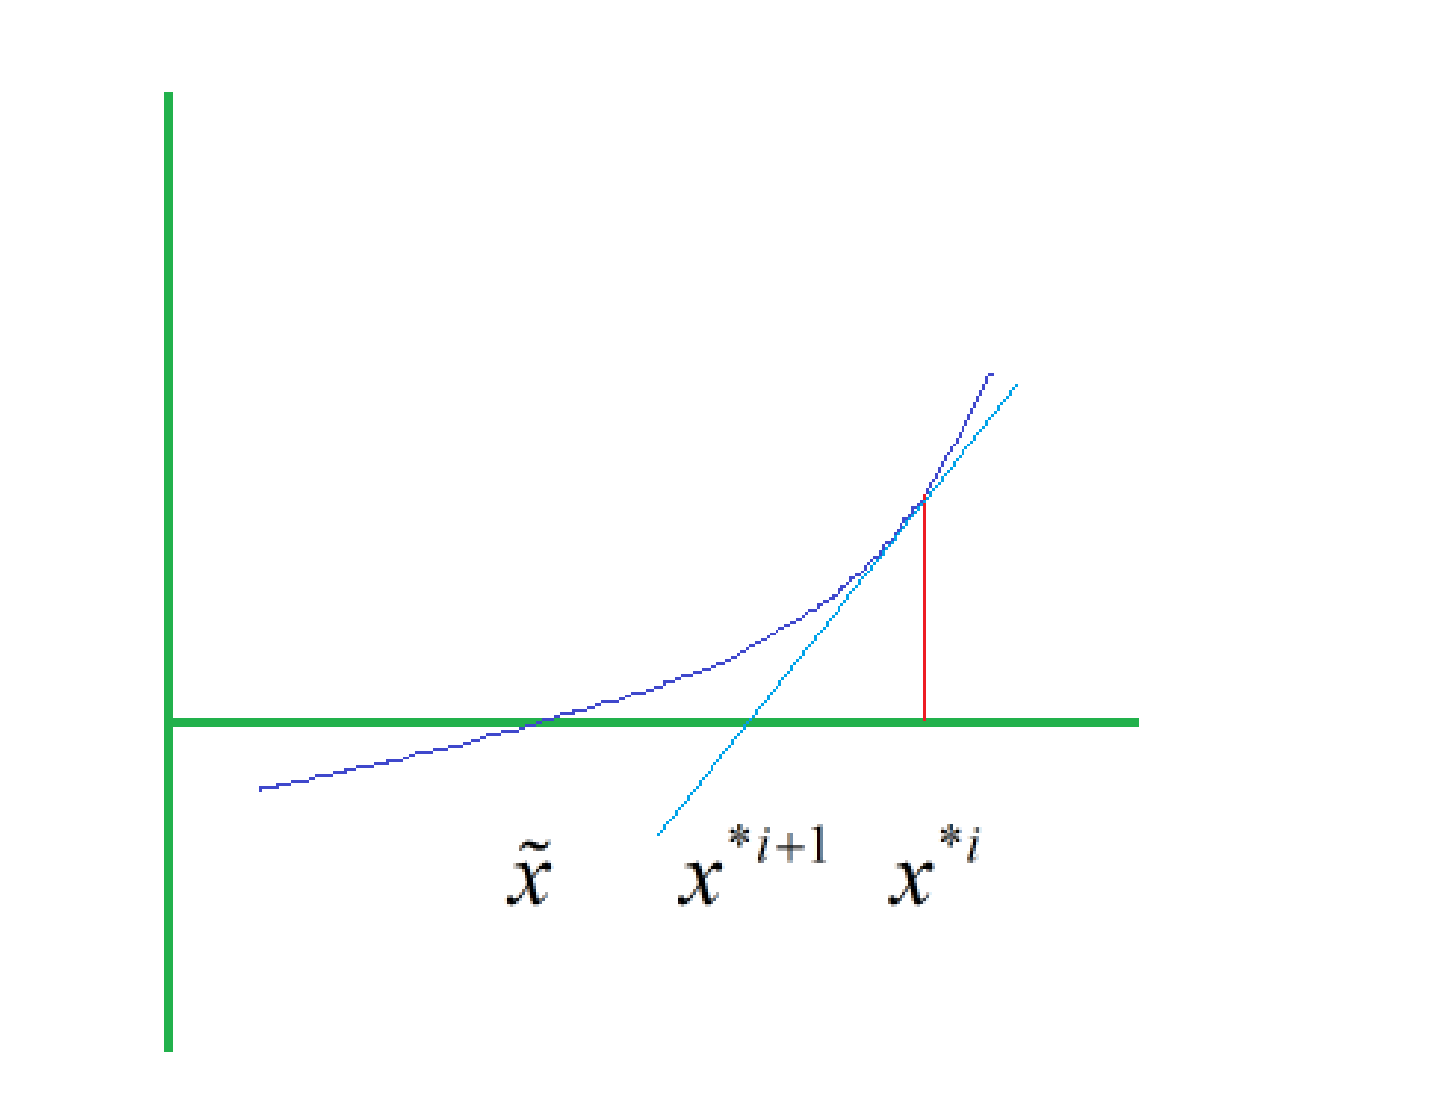
\includegraphics[width=0.7\linewidth]{optimizationNewtonPointClosed0Type0}
\caption{Illustration of the Newton assumption.}
\label{fig:optimizationNewtonPointClosed0Type0}
\end{figure}

We can iteratively compute the point $x^{i + 1}$ from $x^{i}$ till the $f\left(x^{i + 1}\right)$ is very closed to 0 (We do not need the the Newton assumption is always satisfied in every iterative process. We only need the unsatisfied Newton assumption can be turned into satisfied Newton assumption. We call this assumption the partial Newton assumption, as shown in Fig.\ref{fig:optimizationNewtonPointClosed0Type1}. Partial Newton assumption is the sufficient but not necessary conditions for using successively  Newton algorithm to solve equation). This method is called Newton algorithm. Notice that the Newton algorithm will be invalid when the derivation in point $x^{*i}$ is 0, so we must make sure the derivation in initial point (select a good initial point) and every updated point (when the derivation is 0, we need to move the updated point in some offsets) do not be 0. 
However, when the partial Newton assumption is not tenable, then the Newton algorithm may be expected, as illustrated in Fig.\ref{fig:optimizationUnSatisfiedPartialNewtonAssumption}.

\begin{figure}
\centering
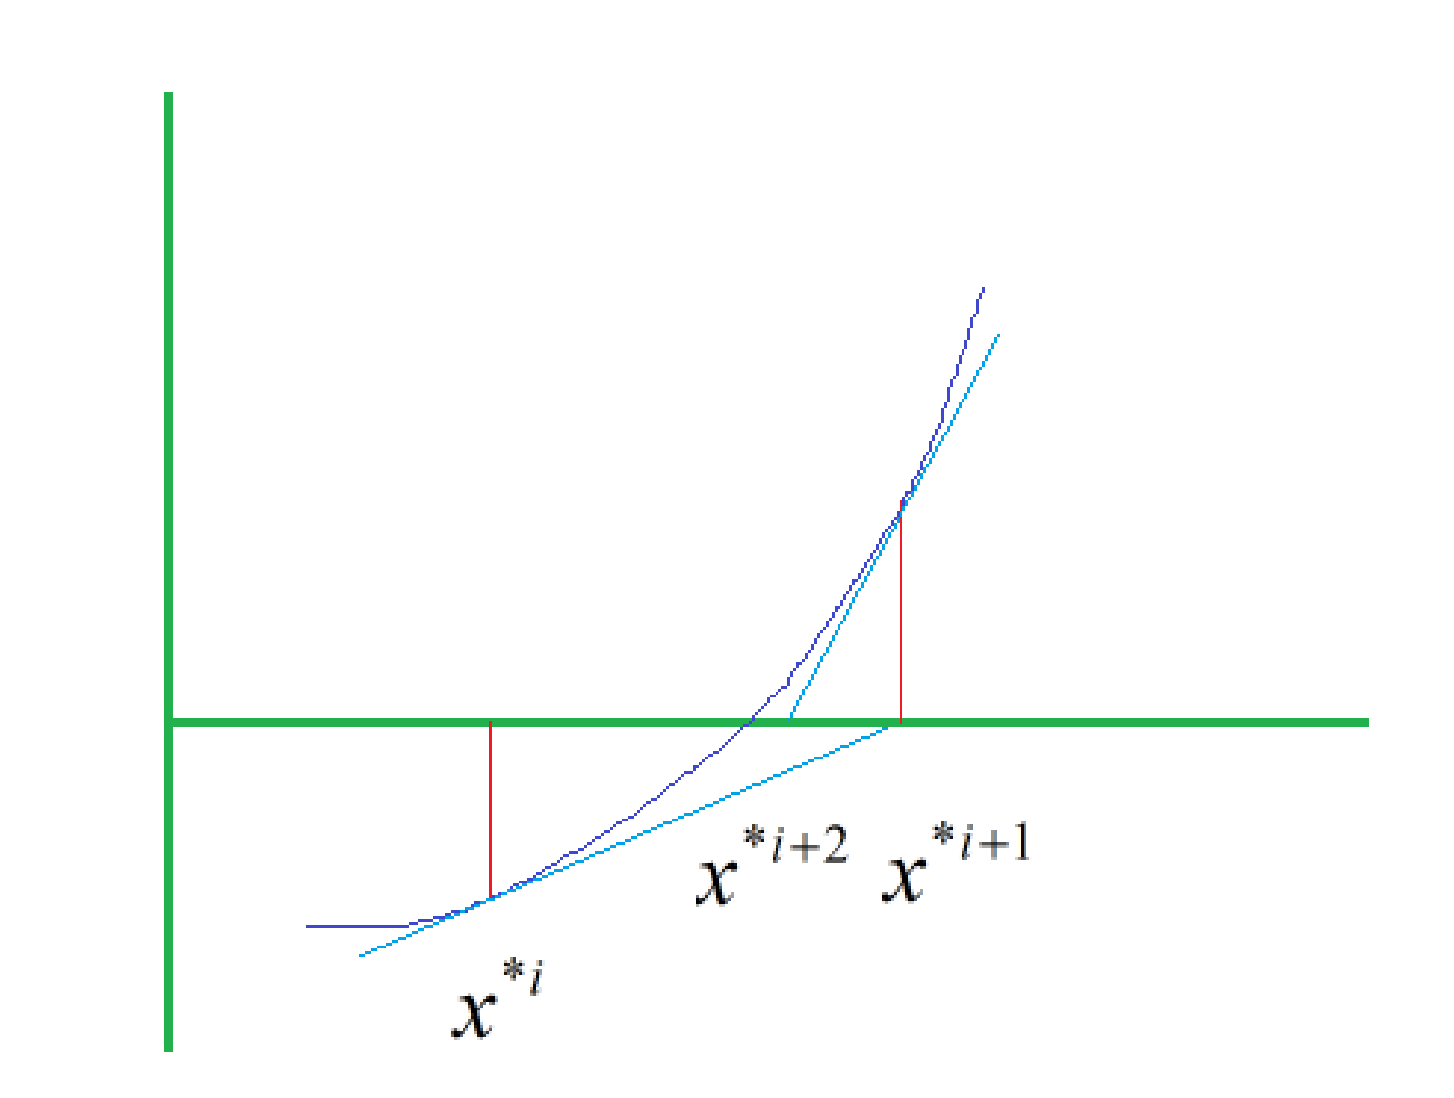
\includegraphics[width=0.7\linewidth]{optimizationNewtonPointClosed0Type1}
\caption{Illustration of the partial Newton assumption.}
\label{fig:optimizationNewtonPointClosed0Type1}
\end{figure}

\begin{figure}
\centering
\subfigure[]{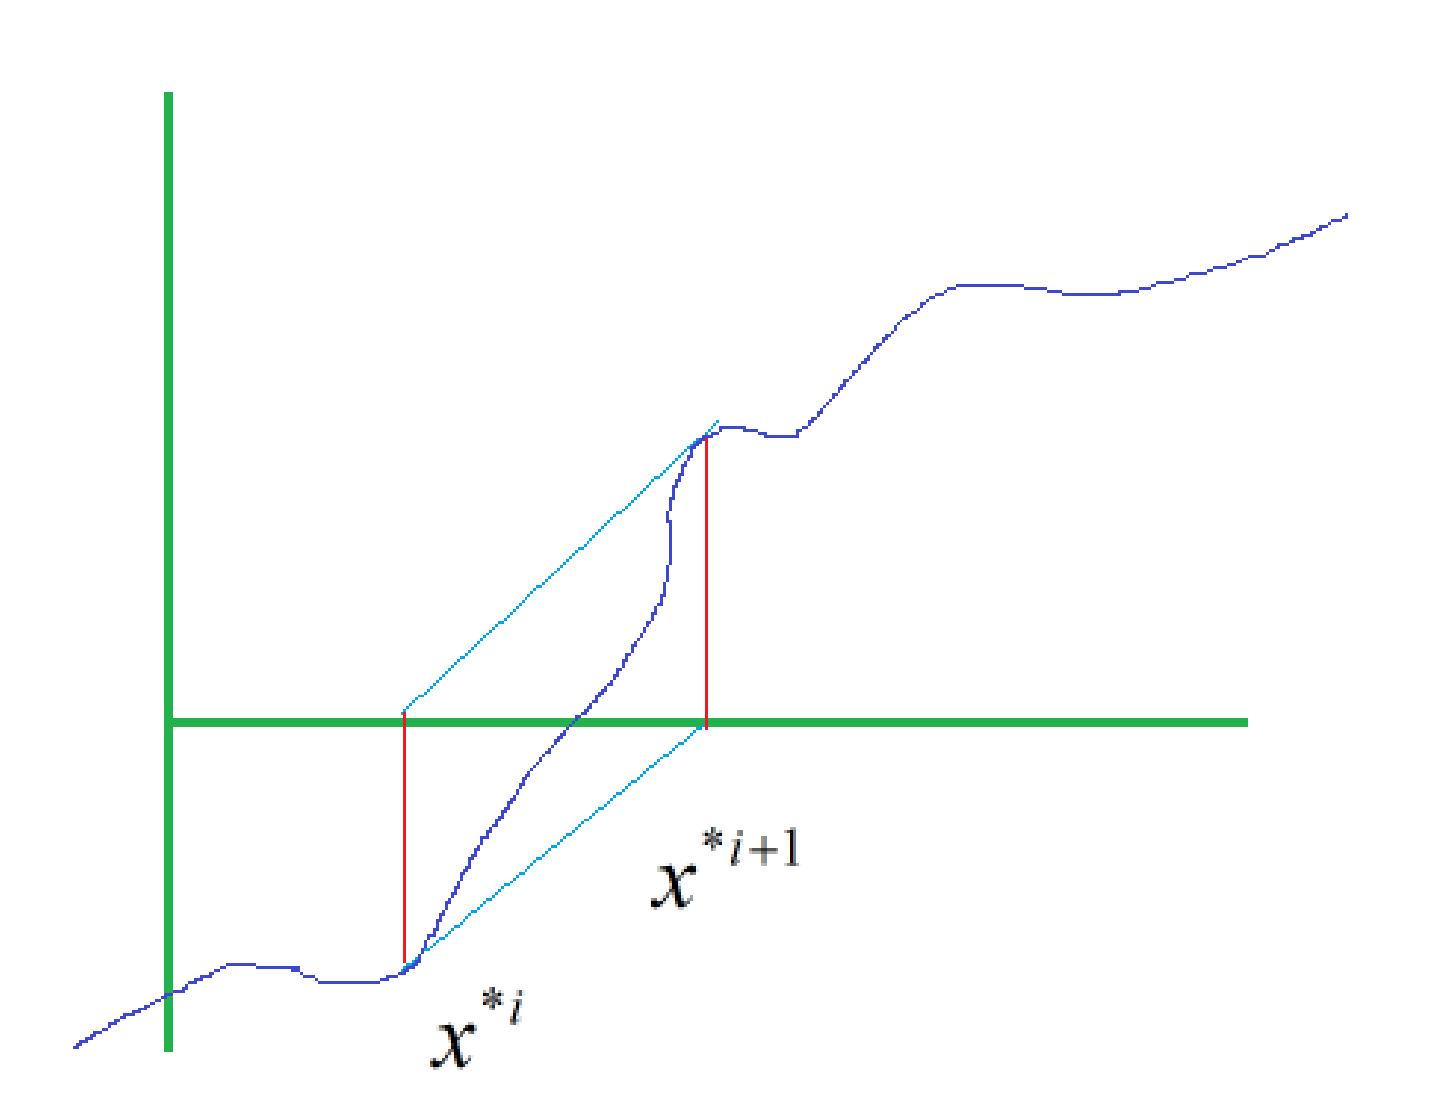
\includegraphics[width=0.48\linewidth]{optimizationNewtonPointInvalid0}}
\subfigure[]{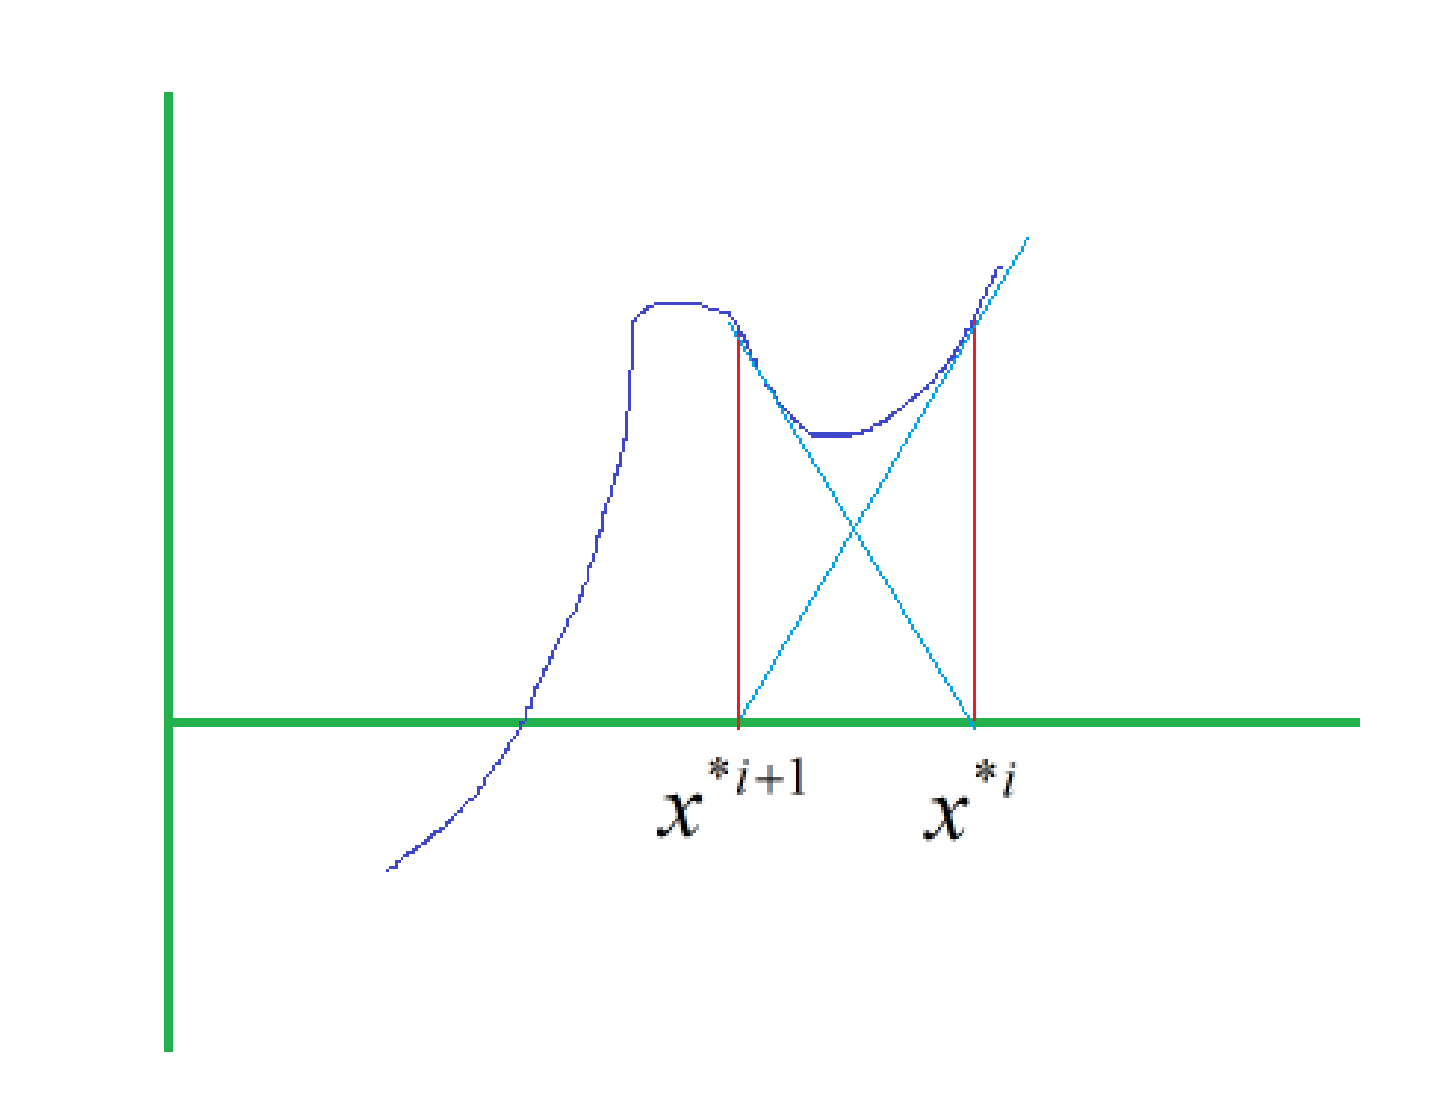
\includegraphics[width=0.48\linewidth]{optimizationNewtonPointInvalid1}}
\caption{Illustration of the unsatisfied partial Newton assumption.}
\label{fig:optimizationUnSatisfiedPartialNewtonAssumption}
\end{figure}

We can apply the Newton algorithm to solve the optimization problems. Since the derivation of point of maximum or minimum value is equal to 0. So Eq.~\ref{equ:optimizationApproximatePoint} can be formatted to Eq.~\ref{equ:optimizationNewtonOptimization}.

\begin{equation}
\label{equ:optimizationNewtonOptimization}
\begin{aligned}
&{f^{'}}\left( x \right) = 0\\
&{f^{'}}\left( x \right) \approx {f^{'}}\left( {{x^{*i}}} \right) + {f^{''}}\left( {{x^{*i}}} \right)\left( {x - {x^{*i}}} \right)\\
\Rightarrow &f^{'}\left( {{x^{*i}}} \right) + {f^{''}}\left( {{x^{*i}}} \right)\left( {x - {x^{*i}}} \right) \approx 0\\
\Rightarrow &\tilde x \approx {x^{*i + 1}} = {x^{*i}} - \frac{{{f^{'}}\left( {{x^{*i}}} \right)}}{{{f^{''}}\left( {{x^{*i}}} \right)}}
\end{aligned}
\end{equation}

Intuitively, Newton optimization algorithm finds the point whose gradient is 0 starting from a given initial point. The value in such point can be either local maximum or minimum value depended on the search direction (defined by $- \frac{{{f^{'}}\left( {{x^{*i}}} \right)}}{{{f^{''}}\left( {{x^{*i}}} \right)}}$). 
Newton algorithm can be considered a special gradient descent/ascend algorithm by taken $|\frac{1}{{{f^{''}}\left( {{x^{*i}}} \right)}}|$ as the learning rate which can make sure the optimization algorithm find the point of local maximum or minimum value under the partial Newton assumption while normal gradient descent/ascend algorithm may require adjust dynamically the learning rate in order to avoid the shake near the point of local maximum or minimum value. 
Notice that Newton optimization algorithm does not make sure the times of update steps is lesser than the gradient descent/ascend algorithm used other setting of learning rate. 
Newton optimization algorithm just provide a feasible setting of learning rate that avoid the workload of designing the mechanism of learning rate.

Since the Newton algorithm need the optimization process (the position of the points, the monotonicity and smoothness of the derivation function of the optimization object function) to satisfy the partial Newton assumption (intuitively, the initial point should be very closed to the point of whose gradient is 0, maybe the point of local maximum or minimum value). However, selecting a good initial point is difficult for many non-convex problems. However, normal gradient descent/ascend algorithm does not need the optimization process to satisfy the partial Newton assumption and it can reach the point near point of local maximum or minimum value (in a small range, the function will has the monotonicity more possibly). So the substitutional way is that we randomly select a initial point and then employ the normal gradient descent/ascend algorithm to find a good initial point for the Newton optimization algorithm, as shown in Fig.\ref{fig:optimizationGradientToNewton}.

\begin{figure}
\centering
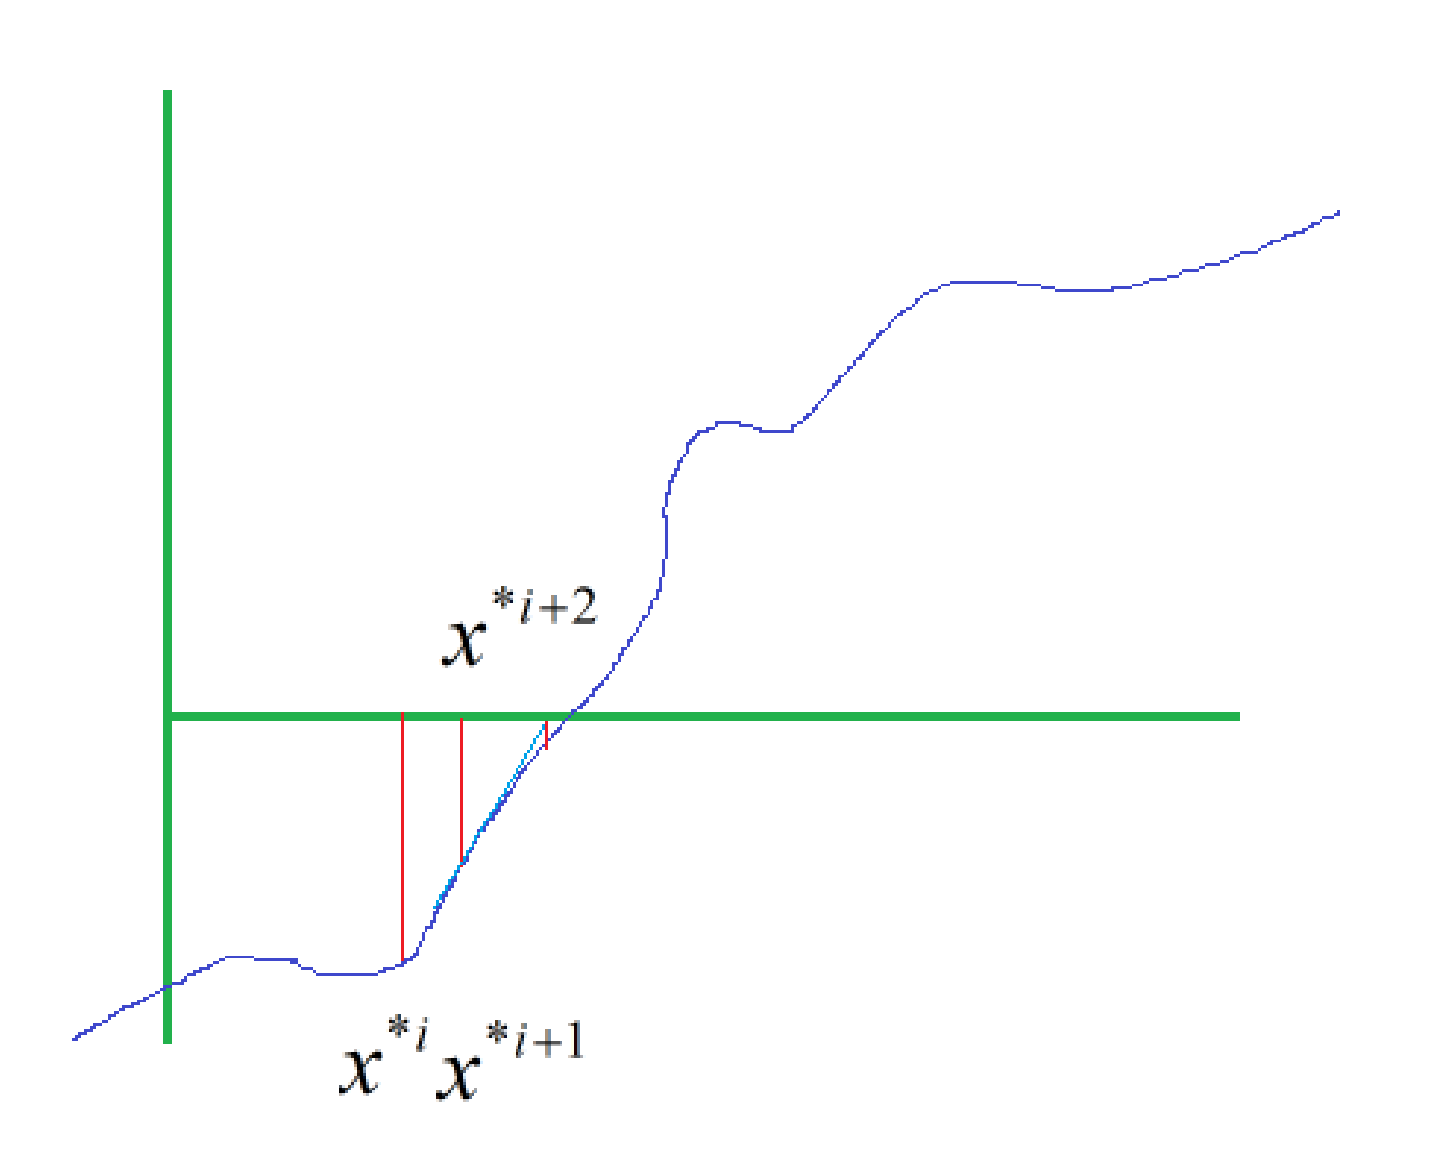
\includegraphics[width=0.7\linewidth]{optimizationGradientToNewton}
\caption{Illustration of the compound method. $x^{i}$ is the initial point for gradient descent algorithm. $x^{i + 1}$ is the iterative point calculated by gradient descent algorithm and is considered the initial point for Newton algorithm. $x^{i + 2}$ is the iterative point calculated by Newton algorithm.}
\label{fig:optimizationGradientToNewton}
\end{figure}

We expand Eq.~\ref{equ:optimizationNewtonOptimization} to multiple dimensions, the calculation can be defined by Eq.~\ref{equ:optimizationNewtonMultipleDimensions}.

\begin{equation}
\label{equ:optimizationNewtonMultipleDimensions}
{x^{*i + 1}} = {x^{*i}} - H{\left( {{x^{*i}}} \right)^{ - 1}}{f^{'}}\left( {{x^{*i}}} \right)
\end{equation}
Where the $H$ is the Hesse matrix.

\subsection{Log Function}
\label{sec:logFunction}
Usually, the optimization object function $J\left(\theta\right)$ consider many training samples in which each training sample $x^{* i}$ can be combined with the parameters $\theta$ to from a optimization factor function $JS\left( {{x^{* i}},\theta } \right)$. So the optimization object function can be formed in two types as Eq.~\ref{equ:optimizationTwoOPTF} shows.

\begin{equation}
\label{equ:optimizationTwoOPTF}
\begin{aligned}
J\left( \theta  \right) &= \prod\limits_{i = 0}^{n - 1} {JS\left( {{x^{* i}},\theta } \right)} \\
J\left( \theta  \right) &= \frac{1}{n}\sum\limits_{i = 0}^{n - 1} {JS\left( {{x^{* i}},\theta } \right)} 
\end{aligned}
\end{equation}
Where the multiplication expression is the optimization object function in maximum likelihood estimation when we consider the function $J$ as probability function.

When we use the iterative way to solve the problem, we need to differentiate the derivation of $J$ corresponding to $\theta$. If we adopt the optimization object function of multiplication type, then the computational process is very complex while the computational process is very simple in addition type (add the each derivation of $f\left( {{x^{* i}},\theta } \right)$ about $\theta$). There is an other reason why we should use the addition type. We always expect the value of optimization object function is scale-invariant for the number of training samples. The scale of training samples should not affect the update values for $\theta$. For a extreme instance, we sample the training samples in 10 times (now the number of training samples is 11 times to original training samples). We desire the update values of parameter are same to the update values in original samples since the training samples dataset has no virtual transformation.

To covert the $J$ to addition type from multiplication type, we can use the log function. Then we divide the number of training sample in order to get scale-invariant optimization object function.

\chapter{Image Process}
\chapter{Audio Process}
\chapter{Video Process}

\chapter{Basic of Machine Learning}
Machine learning is to find the essential rules behind the data. 
Usually, we preform the machine learning algorithm on a training data to generate a machine learning model which can indicates the essence of the training data so that the model can extend to work on the unknown testing data. 
Simple machine learning algorithm can learn the rules that satisfy the majority part of training data while the complex machine learning algorithm can learn the rules which satisfy all the training data even the noise data.
Generally, machine learning can be divide into two types, supervised learning and unsupervised learning. In this section, we will discuss the two types of machine learning.

\section{Supervised Learning}
For supervised learning, the training data have feature data $x$ and response data $y$.
The only target of supervised learning models is to estimate a function $f$ that satisfy the Eq.~\ref{equ:mlSupervisedFunction} on the majority of training data under some assumption (see details in Sec.\ref{sec:lossFunction}).

\begin{equation}
\label{equ:mlSupervisedFunction}
y = f\left( {x,\theta } \right)
\end{equation}
Where $\theta$ is the learning parameter of the function. In many learning models, $\theta$ is explicitly existent such as logistic regression and SVM. While for other models like decision tree and KNN, $\theta$ is hidden under the structure of the learning models.

Consider the type of response, we can divide the supervised learning problems into two categories: regression (response is numerical) and classification (response is discrete). 
It seems that we can directly take the discrete category as continuous response and apply the method adopted in regression. 
However, we always want to know the probability for each category in most times (if we know the probability for each category, we have the abilities to do more custom decision, such as we can get the most possible $kth$ categories). 
Besides, the discrete category is unable to order so that the regression model is improper to treat it as continuous.
Under the assumption of $p\left( {y|x,\theta } \right) = 1$ when labelled response of $x$ is equal to $y$, we can directly convert the classification task to a probability regression task.
However, it may not satisfy the real data distribution so the learning probability regression function may not represent the real probability value.
Besides this assumption is incomplete since the probability only contains two value 1 and 0 ($p\left( {y|x,\theta } \right) = 1$ when labelled response of $x$ is not equal to $y$) that will make the learning more difficult.

Ignoring the difference of structure of models, both regression and classification tasks can be considered a parameter estimation tasks.
Specifically, for a regression task, we can assume the error between labelled response and the predict result $f\left( {x,\theta } \right)$ of model satisfy the Gaussian distribution $N\left( {0,{\sigma ^2}} \right)$.
For a classification task, we directly assume the feature and the response satisfy a distribution $y = p\left( {x,\theta } \right)$.

If we employ MLP method to estimate the parameter, the estimated parameter will lead the predict result $f\left( {x,\theta } \right)$ approximate to the labelled response in regression problems. While for classification problems, the estimated parameter will make $p\left( {y|x,\theta } \right)$ approximate to $1$ when labelled response of $x$ is equal to $y$.
In extreme cases, the approximate property will be identical property when the represent capacities of learning models are very powerful (usually the structures of models are very complex, i.e. models with many parameters).
However, the learning models in such extreme cases are not the best models we want due to they wandered way off the actual data distribution, see details in Sec.~\ref{sec:over_fitting}.
Hence, we usually adopt MAP method to estimate the parameter by add some prior knowledge, such as the parameter should satisfy Gaussian distribution or Laplace distribution, we will discuss the details in Sec.~\ref{sec:lossFunction}.

We named the curve of the function $f\left( {x,\theta } \right)$ of regression curve in regression problems, named the curve of the function $p\left( {y|x,\theta } \right)$ of probability regression curve in classification and named the curve, the projection at the discriminant probability threshold (usually is 0.5) of the probability regression curve to the feature space, of discriminant curve. Fig.~\ref{fig:mlRelationOfDR} shows an example of discriminant curve and the corresponding probability regression curve in a binary classification problem. 

\begin{figure}
\centering
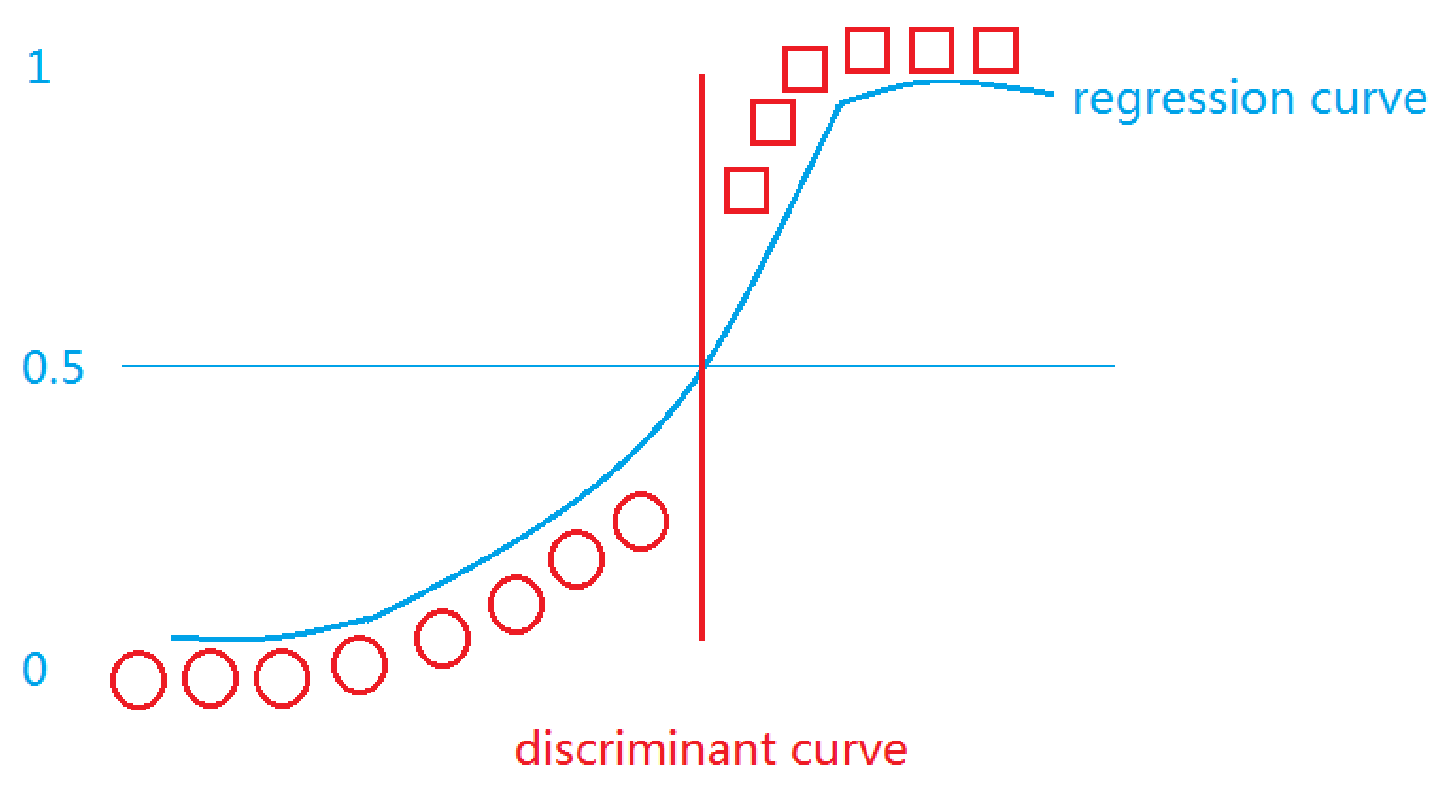
\includegraphics[width=0.7\linewidth]{mlRelationOfDR}
\caption{Illustration of the relation between discriminant curve and probability regression curve. The discriminant curve is in feature space, here the feature is 1-dimension. The probability regression curve is in feature and response space, here the response of category is the probability in the range of $\left(0, 1\right)$.}
\label{fig:mlRelationOfDR}
\end{figure}

Many machine learning models can preform both regression and classification. On the bias of the representation form of function $f$, we divide the supervised learning models into four categories: discriminant/regression (\emph{DR}) curve based models (i.e. linear regression, logistic regression, softmax, perceptron or multilayer perceptron, recurrent neural network, SVM), bayes based models, decision tree based models (i.e. decision tree, random forest and adaboost) and neighbourhood based models. The functions $f$ are explicit for discriminant/regression curve based models while are hidden in other models. For instance, the $f$ in decision tree based model are hidden in the series of decision rules. We will discuss the details for the three models in following sections. 

\section{Unsupervised Learning Models}
For unsupervised learning, the training data only have feature data. 
The main target of unsupervised learning model is to find the essence of training data in feature space. 
Generally, the unsupervised learning models can be roughly divided into two categories: cluster and representation. 
Specifically, for cluster, we want to cluster the training data into several categories. For representation, we want to find the most useful representation for the original feature, that is to say, convert the original feature to the new feature space which is more effective to represent the data.

\section{Training Data}
\label{sec:training_data}
For a machine learning problem, we need to collect as many as possible training data for the learning model.
Here we categorize training data into three types: perfect training data, imperfect training data and terrible training data.
For perfect training data, it provides whole possibility of real data in the corresponding feature space and has no noise inside.
While the imperfect training data provides majority of possibility of real data in the feature space and has little noise.
For terrible training data, it lost many possibility of real data and contains too much noise inside.

Given a training data, if it is perfect training data, we can employ the best learning model to train it and achieve a wonderful learning result in the feature space (note that the wonderful learning result is for the feature space the training data belongs to. It may not be the practice result we want if the feature space is defective).
However, we can't acquire enough training data in most times and the given training data usually has noise. 
Thus the practice object of training data collection is to collect the imperfect training data.

The noise in supervised problems can be divided into two types: wrong feature and wrong category.
For wrong feature noise data, its feature does not belong to the feature space of the correct training data.
For wrong category noise data, its feature belongs to the correct feature space while the labelled category is wrong.

On the basis of the independence of different dimensions of feature, we categorize feature into two types: heterogeneous feature and isomorphic feature.
For heterogeneous feature, we can consider different dimensions of feature are independent. Usually, they represent different aspect of object and are high level with strong semantic.
While for isomorphic feature, different dimensions of feature are in-independent. Usually, they are compute by the same feature extraction algorithm (such as HOG, SIFT or even pixel value) and low level with low semantic.
For heterogeneous feature, we should select the learning models that can handle them well, such as decision tree based models. While for isomorphic feature, we better select the learning models such as DR based models since DR based models learn a DR function to fit the training data that combine each dimension of isomorphic feature.

\section{Unbalanced Learning}
\label{sec:unbalanced_learning}
For a perfect or imperfect training data in classification, if the training samples of different category are in a large variety of scale, the learning problem turns to a unbalanced learning.
If we have a super learning model that can classify every training sample correctly, we do not need care the problem of unbalanced learning.
However, such learning model are difficult to obtain (it is difficult to train or we restrict complexity of the model to deal with over-fitting problem). In most times, learning model may sacrifice some fitting performance on some training training samples. The training samples of low scale category are most likely to be sacrifice.
If the learning object is to learn a model that can get a total precision on all categories, then the unbalanced learning will not bring any problems for us.
While if we we prefer the precision and recall on each category, the unbalanced learning may cause a serious problem that the precision or recall result on the low scale category may be evidently terrible.

For unbalanced learning in MLPs and SVMs, since the optimal object is minimizing the loss function which is computed use all training data (for MLPs, even corrected labelled training samples also have loss value for loss function while only uncorrected labelled training samples contribute the loss function), when the model sick a situation that it must sacrifice some training samples, it trend to sacrifice the training samples of low scale category due to diverging the discriminant curve forward training samples of low scale category is costly, as shown in Fig.~\ref{fig:unbalanced_learning_mlp_svm}. 
For unbalanced learning in decision trees, it is easy to see that the training samples of low category in leaf node is minor (we usually restrict complexity of the decision trees to handle over-fitting problem, so the decision trees will stop split in early time). Hence the decision trees trend ignore them by adopt the major categories.

\begin{figure}
\centering
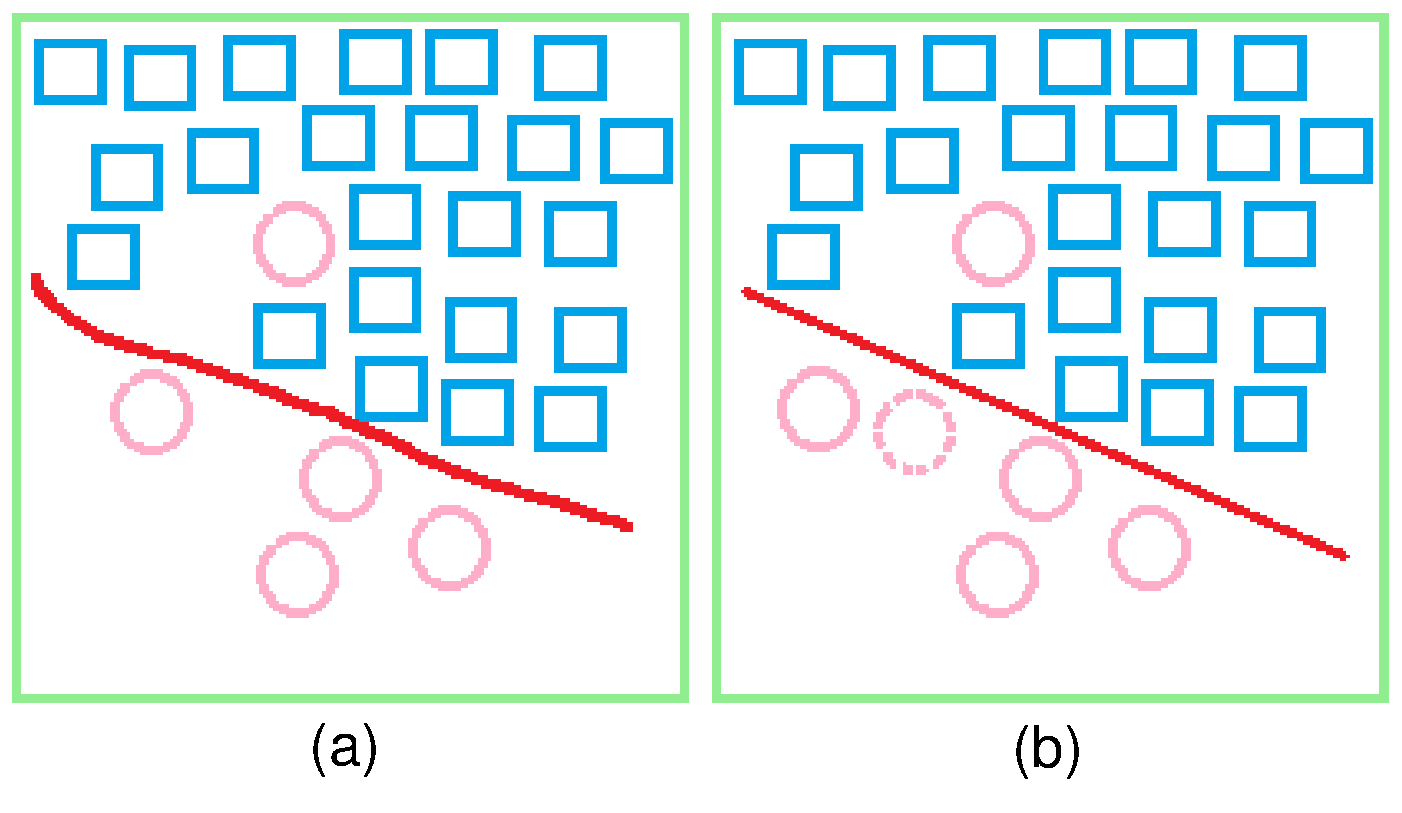
\includegraphics[width=0.7\linewidth]{unbalanced_learning_mlp_svm}
\caption{Illustration of the unbalanced learning in (a )MLPs  and (b) SVMs.}
\label{fig:unbalanced_learning_mlp_svm}
\end{figure}

Generally speaking, training samples of low scale category usually are considered noise for training data and will be processed by some skills (restricting complexity of models) to eliminate their influence for learning models.
Thus if we we prefer the precision and recall on each category, we need train our model in the balanced training data (usually the ratio of the number of the largest scale category divided by the number of the smallest scale category should below $5$).

\section{Over-fitting}
\label{sec:over_fitting}
For a supervised machine learning problem, a learning model under MLP parameter estimation method may fit all the training samples so that the training error is very negligible (actually, ignoring the error response in two same samples, a sufficient complex learning model has the ability to fit all training samples in extreme environment). We call this situation over-fitting training. 

The complexity of learning model and the corresponding learning problem decide together the over-fitting whether to occur. Over-fitting training only take place in the situation when the learning model is more complex than the learning problem. 
Specifically, when face a very simple linear regression problem (the training data is linear separation in feature space), the simple linear regression model can train on the problem with over-fitting. For a complex learning problem, such as face recognition, the training data is very complex, thus we need a complex learning model to learn it that we can over-fitting the learning data. Using a logistic regression model to learn the face recognition problem will not be over-fitting.   

When the training data is sufficient to reflect the real data distribution and there is no noise inside, we can always employ a complex learning model (with effective learning algorithm) to learn the training data. The learned model will be perfect on the predicting task.
However, we can't acquire enough training data in most times and the given training data usually have noise.
If the training data is terrible training data, the learning result will be very bad and can not be adjusted. 
Besides, simple learning models can't train the training data of most learning problem in over-fitting type in most times and simple models have no necessity to adjust for avoid over-fitting training since they are already simple. 
Thus we only discuss the complex learning models on imperfect training data.
For the imperfect training data (lost little possibility and contains little noise), if the learning model learns it in over-fitting type, the learned model maybe imperfect for the corresponding predicting task even the learning result is perfect in training task.
We will discuss the problems of over-fitting training machine learning models in each section of learning model.

The over-fitting in perfect training data is good for the learning models. 
However, the training data is insufficient and noisy in common, the over-fitting training on imperfect training data may cause some defects for our learning models. We can adopt some skills on the learning models to avoid the over-fitting so that the defects can be eliminated.

For a complex learning model, it has high probability to sick in over-fitting training. 
For a simple learning model, if the learning problem is complex, it can't work well on training data so that it has no way to sick in over-fitting training. Otherwise, even though the easy learning model may sick in over-fitting training in a easy learning problem, consider the model is already simple, so we don't need to avoid the over-fitting (such as logistic and softmax regression models).

Avoiding the over-fitting training does not ensure that the predict performance will be improved due to the assuming precondition that the DR curve is smooth  (learning models should be not too complex) for real data distribution. However, when apply the skills for avoiding over-fitting training for such complex models, the predict performance have high probability to be the better.

\section{Bias and Variance}
Given:\footnote{This section references from The Bias-Variance Tradeoff from internet.}

- the true function we want to approximate

\begin{displaymath}
g=g\left(x\right)
\end{displaymath}

-the data set for training

\begin{displaymath}
D_t=\left[\left(x^{*0},y^{*0}\right),\left(x^{*1},y^{*1}\right),...,\left(x^{*M-1},y^{*M-1}\right)\right]\quad where\ y = g + \varepsilon\ and\ E\left(\epsilon\right)=0
\end{displaymath}

-the data set for testing

\begin{displaymath}
D_p=\left[\left(x^{*0},y^{*0}\right),\left(x^{*1},y^{*1}\right),...,\left(x^{*N-1},y^{*N-1}\right)\right]\quad where\ y = g + \varepsilon\ and\ E\left(\epsilon\right)=0
\end{displaymath}

- given ${D_t}$, we train an arbitrary model to approximate the function $f$ by

\begin{displaymath}
o=f\left(x,\theta\right)
\end{displaymath}
note that the output value ${o}$ is a variable but not a deterministic value due to the response is a variable!

The mean-squared error of this model for testing dataset ${D_p}$ is:

\begin{displaymath}
MSE=\frac{1}{N}{\sum_{i=0}^{N-1}\left ( y^{*i}-o^{*i} \right )^2}
\end{displaymath}

To evaluate the predicting ability of the learning algorithm (notice that the learning algorithm is different from the learned model. For the learning algorithm, it includes the learning strategy and the initial configuration. While for the learned model, it is the learning result for a algorithm learned on a training dataset), we want to know the expectation of the training MSE of the model trained on the training dataset $D_t$ predict on $D_p$.

%we want to know the expectation of the MSE if we want test the model on arbitrary many test samples drawn from the unknown function $g\left(x\right)$ independently.
%For instance, we train a model on a given training dataset, then we evaluate it on several testing datasets. Then we acquire several MSE computed on the testing dataset. We take each MSE for a given testing dataset as a random variable, then calculate the expectation of the MSE variable.

\begin{displaymath}
E\left ( MSE \right )=E\left \{ \frac{1}{N} {\sum_{i=0}^{N-1}\left ( y^{*i}-o^{*i} \right )^2}\right \}
=\frac{1}{N}{\sum_{i=0}^{N-1}{E\left ( y^{*i}-o^{*i} \right )^2}}
\end{displaymath}

Let's investigate the expectation inside the sum, with a little "augmentation trick":

\begin{displaymath}
\begin{aligned}
E\left ( y^{*i}-o^{*i} \right )^2&=E\left ( y^{*i}-g^{*i}+g^{*i}-o^{*i} \right )^2\\
&=E\left ( y^{*i}-g^{*i} \right )^2+E\left ( g^{*i}-o^{*i} \right )^2+2E\left \{ \left ( y^{*i}-g^{*i} \right )\left ( g^{*i}-o^{*i} \right )\right \}\\
&=E\left \{ \left(\varepsilon^{*i}\right)^2  \right \}+E\left \{\left ( g^{*i}-o^{*i} \right )^2\right \}+\\
&\quad\quad 2\left \{ E\left ( y^{*i}g^{*i} \right ) -E\left ( y^{*i}o^{*i} \right )-E\left ( \left ( g^{*i} \right )^2 \right ) +E\left ( g^{*i}o^{*i} \right )\right \}
\\
\end{aligned}
\end{displaymath}

Note that:

\begin{displaymath}
E\left ( y^{*i}g^{*i} \right )=g^{*i}E\left ( y^{*i} \right )=g^{*i}E\left ( g^{*i}+\varepsilon^{*i}  \right )=\left ( g^{*i} \right )^2
\end{displaymath}
since $g$ is deterministic.

And

\begin{displaymath}
E\left \{ \left ( g^{*i} \right )^2 \right \}=\left ( g^{*i} \right )^2
\end{displaymath}
since $g$ is deterministic.

And

\begin{displaymath}
\begin{aligned}
E\left ( y^{*i}o^{*i} \right )&=E\left \{ \left ( g^{*i}+\varepsilon^{*i} \right )o^{*i} \right \}\\
&=E\left (g^{*i}o^{*i} \right )+E\left ( \varepsilon^{*i} o^{*i} \right )\\
&=E\left (g^{*i}o^{*i} \right )+E\left ( \varepsilon^{*i} \right )E\left ( o^{*i} \right )\\
&=E\left (g^{*i}o^{*i} \right )
\end{aligned}
\end{displaymath}
since we consider the $\varepsilon$ is independent of the model prediction.

Thus the MSE can be decomposed in expectation into the variance of the noise ($E\left ( \varepsilon^2  \right ) = D\left ( \varepsilon  \right )$ due to $E\left ( \varepsilon  \right )=0$) and the MSE between the true function and the predicted values.

\begin{displaymath}
E\left ( y^{*i}-o^{*i} \right )^2 = E\left \{ \left(\varepsilon^{*i}\right)^2  \right \} +E\left \{\left ( g^{*i}-o^{*i} \right )^2\right \}
\end{displaymath}

This term can be further composed with the same augmentation trick as above.

\begin{displaymath}
\begin{aligned}
E\left ( g^{*i}-o^{*i} \right )^2 &= E\left \{\left ( g^{*i} - E\left ( o^{*i} \right )+E\left ( o^{*i} \right ) - o^{*i}\right )^2 \right \}\\
&=E\left \{ \left \{ g^{*i} - E\left ( o^{*i} \right ) \right \}^2 \right \}+E\left \{ \left \{ o^{*i} - E\left ( o^{*i} \right ) \right \}^2 \right \}+\\
&\quad\quad 2\left \{ E\left \{ g^{*i}E\left ( o^{*i} \right ) \right \} - E\left \{ E\left ( o^{*i} \right )^2 \right \} - E\left \{ g^{*i}o^{*i} \right \}+ E\left \{ E\left ( o^{*i} \right )o^{*i} \right \}\right \}
\end{aligned}
\end{displaymath}

Note that:

\begin{displaymath}
\begin{aligned}
E\left \{ g^{*i}E\left ( o^{*i} \right ) \right \}&=g^{*i}E\left ( o^{*i} \right )\\
E\left \{ E\left ( o^{*i} \right )^2 \right \}&=E\left ( o^{*i} \right )^2\\
E\left \{ g^{*i}o^{*i} \right \}&=g^{*i}E\left ( o^{*i} \right )\\
E\left \{ E\left ( o^{*i} \right )o^{*i} \right \}&=E\left ( o^{*i} \right )E\left ( o^{*i} \right )
=E\left ( o^{*i} \right )^2
\end{aligned}
\end{displaymath}

Hence we acquire:

\begin{displaymath}
\begin{aligned}
E\left ( g^{*i}-o^{*i} \right )^2 =E\left \{ \left \{ g^{*i} - E\left ( o^{*i} \right ) \right \}^2 \right \}+E\left \{ \left \{ o^{*i} - E\left ( o^{*i} \right ) \right \}^2 \right \}
\end{aligned}
\end{displaymath}

Thus the decomposition of the MSE in the expectation becomes:

\begin{displaymath}
\begin{aligned}
E\left ( y^{*i}-o^{*i} \right )^2&=E\left ( \left(\varepsilon^{*i}\right)^2  \right )+E\left \{ \left \{ g^{*i} - E\left ( o^{*i} \right ) \right \}^2 \right \}+E\left \{ \left \{ o^{*i} - E\left ( o^{*i} \right ) \right \}^2 \right \}\\
&=var\left(noise\right) + bias^2 + var\left(o^{*i}\right)
\end{aligned}
\end{displaymath}

Note that the variance of the noise can not be minimized; it is independent of the model.
Thus in order to minimize the MSE, we need to minimize both the bias and the variance.
However, this is not trivial to do this. For instance, just neglecting the input data and predicting the output somehow (e.g., just a constant), would defonitely minimize the variance of our predictions: they would be always the same, thus the variance would be zero - but the bias of the estimate (i.e., the amount we are off the real function) would be tremendously large. 
On the other hand, the model could perfectly interpolate the training data, i.e., it predict $o=y$ for every testing sample. 
This will make the bias term vanish entirely, since the $E\left(o\right)=E\left(y\right)=g$, but the variance term will become equal to the variance of the noise, since 

\begin{displaymath}
\begin{aligned}
E\left \{ \left ( o - E\left ( o \right ) \right )^2 \right \}&=E\left \{ \left ( y - E\left ( y \right ) \right )^2 \right \}\\
&=E\left \{ \left ( y - E\left ( g \right ) \right )^2 \right \}\\
&=E\left \{ \left ( y - g\right )^2 \right \}\\
&=E\left \{ \varepsilon ^2 \right \}
\end{aligned}
\end{displaymath}

\subsubsection{Bias and Variance for Bagging Algorithm}
Bagging Algorithm obtains the lower variance comparing with the corresponding base algorithm, while the bias is not changed. Since the bagging strategy adopt the random strategy for sampling the training dataset, the child models trained by the base algorithm for a bagging algorithm can be considered independently. Let $\left(o^{*i} \right)^{*j}$ denotes the output of $j$th child trained model predicting on the $i$th predicting sample. Then the output of bagging model:

\begin{displaymath}
\frac{\sum_{j=0}^{K-1}\left ( o^{*i} \right )^{*j}}{K}
\end{displaymath}
where $K$ is the child models number for the bagging algorithm.

Then the variance term for the bagging algorithm can be 

\begin{displaymath}
\begin{aligned}
E\left \{ \left \{ \frac{\sum_{j=0}^{K-1}\left ( o^{*i} \right )^{*j}}{K}
 - E\left ( \frac{\sum_{j=0}^{K-1}\left ( o^{*i} \right )^{*j}}{K}
 \right ) \right \}^2 \right \}&=D(\frac{\sum_{j=0}^{K-1}\left ( o^{*i} \right )^{*j}}{K})\\
 &=\frac{\sum_{j=0}^{K-1}\left ( D(o^{*i})^{*j} \right )}{K^2}\\
 &=\frac{D(o^{*i})^{*0}}{K} = \frac{D(o^{*i})^{*1}}{K} = ... = \frac{D(o^{*i})^{*K-1}}{K}
\end{aligned}
\end{displaymath}

While for the bias term 

\begin{displaymath}
\begin{aligned}
E\left \{ \left \{ g^{*i} - E\left ( \frac{\sum_{K-1}^{j=0}\left ( o^{*i} \right )^{*j}}{K}
 \right ) \right \}^2 \right \}&=E\left \{ \left \{ g^{*i} - E\left ( \left ( o^{*i} \right )^{*0} \right ) \right \}^2 \right \}\\
 &=...\\
 &=E\left \{ \left \{ g^{*i} - E\left ( \left ( o^{*i} \right )^{*K-1} \right ) \right \}^2 \right \}
\end{aligned}
\end{displaymath}


\subsubsection{Bias and Variance for Boosting Algorithms}
The boosting algorithm is a type of forward step optimal algorithm, hence the final output $o^{*i}$ of the algorithm (combination of all the child trained models) tend to have the value that is very close to $y^{*i}$. So the bias term will be reduced comparing to one trained model in the child models. 
However the variance term will not be reduced, even it may be more large if the noise of the testing dataset is larger than the variance term calculated by one trained model (refer to the analysis in before that the boosting model predict $o=y$)!

\subsubsection{Dataset with No Noisy}
What if the training dataset has no noisy? 
We can easily find that the variance term will be zero! Since the output of trained model will be deterministic!
What if the testing dataset has no noisy?
The answer is the $var\left(noise\right)$ will be zero!

\chapter{DR Curve Based Models}

\section{Loss Function}
\label{sec:lossFunction}
For any supervised machine learning problems (no matter the problem is regression or classification), the only object is to fit the regression function to the response or probability of training data under some assumption (such as the model should be simple in order to avoid over-fitting training). To measure the degree of fitting in DR curve based models (loss function exist in DR models), we introduce the loss function which is derived from the estimation of probability distribution. The total loss on training data should be very small, that is to say the error between response or probability and prediction result should be very small in sum and low in variance (so we can assume the error satisfy $N\left( 0, \sigma ^2 \right)$). Specifically, one supervised learning model can be considered one category of probability distribution under reasonable assumption. The learning algorithm is to estimate the parameters (usually, we use MLE or MAP as described in Sec.\ref{sec:parameter_estimation}) of the category of probability distribution. 

Let $y$ denotes the response or probability, $\tilde{y}$ denotes the predict result of learning models, $\varepsilon$ denotes the error between $y$ and $\tilde{y}$. We assume $\varepsilon$ satisfies the Gaussian distribution $N\left( {0,{\sigma ^2}} \right)$. Using the MLE then we have the Eq.~\ref{equ:lossFunctionSuareLossMLE}.

\begin{equation}
\label{equ:lossFunctionSuareLossMLE}
\begin{aligned}
&\left\{ {\begin{array}{*{20}{c}}
{\varepsilon  = y - \tilde y}\\
{\varepsilon  \sim N\left( {0,{\sigma ^2}} \right)}
\end{array}} \right.\\
 \Rightarrow &p\left( \varepsilon  \right) = {\left( {2\pi } \right)^{ - \frac{1}{2}}}{\left( {{\sigma ^2}} \right)^{ - \frac{1}{2}}}\exp \left\{ { - \frac{1}{2}\left( {y - \tilde y} \right){{\left( {{\sigma ^2}} \right)}^{ - 1}}\left( {y - \tilde y} \right)} \right\}\\
 \Rightarrow &P\left( \varepsilon  \right) = \prod\limits_{i = 0}^{n - 1} {p\left( {{\varepsilon ^{*i}}} \right)} \\
 \Rightarrow &\log P\left( \varepsilon  \right) = \sum\limits_{i = 0}^{n - 1} {\log p\left( \varepsilon  \right)} \\
 &\quad\quad\quad\quad= \sum\limits_{i = 0}^{n - 1} {\log {{\left( {2\pi } \right)}^{ - \frac{1}{2}}}{{\left( {{\sigma ^2}} \right)}^{ - \frac{1}{2}}}\exp \left\{ { - \frac{1}{{2{\sigma ^2}}}{{\left( {{y^{*i}} - {{\tilde y}^{*i}}} \right)}^2}} \right\}} \\
 &\quad\quad\quad\quad= \sum\limits_{i = 0}^{n - 1} {\left( {\log {{\left( {2\pi } \right)}^{ - \frac{1}{2}}}{{\left( {{\sigma ^2}} \right)}^{ - \frac{1}{2}}} - \frac{1}{{2{\sigma ^2}}}{{\left( {{y^{*i}} - {{\tilde y}^{*i}}} \right)}^2}} \right)} \\
 \Rightarrow &\max \frac{1}{n}\log P\left( {y} \right) \sim \max \frac{1}{n}\sum\limits_{i = 0}^{n - 1} {\left( { - \frac{1}{{2{\sigma ^2}}}{{\left( {{y^{*i}} - {{\tilde y}^{*i}}} \right)}^2}} \right)}  \\
 \sim &\min \frac{1}{n}\sum\limits_{i = 0}^{n - 1} {\frac{1}{2}{{\left( {{y^{*i}} - {{\tilde y}^{*i}}} \right)}^2}} \\
 \sim &\min \frac{1}{n}\sum\limits_{i = 0}^{n - 1} {\frac{1}{2}{{\left( {{\varepsilon ^{*i}}} \right)}^2}} 
\end{aligned}
\end{equation}

We can see that the quadratic loss function is derived from MLE. In order to make the probability distribution of $p\left(y\right)$ to be maximum, we need the variance of error to be minimum which corresponds to the assumption
\begin{displaymath}
{\varepsilon  \sim N\left( {0,{\sigma ^2}} \right)}.
\end{displaymath}

If we suppose the error satisfy the probability distribution defined by Eq.~\ref{equ:lossFunction01ProbabilityDistribution}.

\begin{equation}
\label{equ:lossFunction01ProbabilityDistribution}
\left\{ {\begin{array}{*{20}{c}}
{p\left( {\varepsilon  = 0} \right) = 1}\\
{p\left( {\varepsilon  \ne 0} \right) = 0}
\end{array}} \right.
\end{equation}

After applying the MLE for this, we will get the 0-1 loss function as described in Eq.~\ref{equ:lossFunction01Loss}.

\begin{equation}
\label{equ:lossFunction01Loss}
\begin{aligned}
&P\left( y \right) = \prod\limits_{i = 0}^{n - 1} {p\left( {{y^{*i}}} \right)}  = \prod\limits_{i = 0}^{n - 1} {\left( {y = \tilde y?1:\frac{1}{{n + 1}}} \right)} \\
&\max \frac{1}{n}\log P\left( y \right) = \max \frac{1}{n}\sum\limits_{i = 0}^{n - 1} {\log \left( {y = \tilde y?1:\frac{1}{{n + 1}}} \right)} \\
 &\quad\quad\sim \max \frac{1}{n}\sum\limits_{i = 0}^{n - 1} {\left( {y = \tilde y?1:\frac{1}{{n + 1}}} \right)} \\
 &\quad\quad\sim \max \frac{1}{n}\left( {\left( {n - \sum\limits_{i = 0}^{n - 1} {\left( {y \ne \tilde y} \right)} } \right) + \frac{{\sum\limits_{i = 0}^{n - 1} {\left( {y \ne \tilde y} \right)} }}{{n + 1}}} \right)\\
 &\quad\quad\sim \max \frac{1}{n}\left( {n - \sum\limits_{i = 0}^{n - 1} {\left( {y \ne \tilde y} \right)} \left( {1 - \frac{1}{{n + 1}}} \right)} \right)\\
 &\quad\quad\sim \min \frac{1}{n}\sum\limits_{i = 0}^{n - 1} {\left( {y \ne \tilde y} \right)} 
\end{aligned}
\end{equation}

For classification problems, the probability for each category is unknown. So we can not assume the probability distribution of the error between probability and prediction result. However, we can assume the conditional probability for each category. Then we have the log loss function as described in Eq.~\ref{equ:lossFunctionLog}.

\begin{equation}
\label{equ:lossFunctionLog}
\begin{aligned}
P\left( {y|x} \right) &= \prod\limits_{i = 0}^{n - 1} {p\left( {{y^{*i}}|{x^{*i}}} \right)} \\
\max \frac{1}{n}\log P\left( {y|x} \right) &= \max \frac{1}{n}\sum\limits_{i = 0}^{n - 1} {\log } p\left( {{y^{*i}}|{x^{*i}}} \right)
\end{aligned}
\end{equation} 

Hence we obtain the logarithmic loss function as defined by Eq.~\ref{equ:loss_function_logarithmic}.

\begin{equation}
\label{equ:loss_function_logarithmic}
\min  - \frac{1}{n}\sum\limits_{i = 0}^{n - 1} {\log p\left( {{y^{*i}}|{x^{*i}}} \right)} 
\end{equation}

If we use the following $p\left ( y|x \right )$ to represent the probability, then we will have the exponential loss as Eq.~\ref{equ:exponential_loss}.

\begin{displaymath}
\begin{aligned}
p\left ( y=1|x \right )&=\frac{exp\left ( -exp\left ( -\tilde{y} \right ) \right )}{exp\left ( -exp\left ( \tilde{y} \right ) \right ) + exp\left ( -exp\left ( -\tilde{y} \right ) \right )}\\
p\left ( y=-1|x \right )&=\frac{exp\left ( -exp\left ( \tilde{y} \right ) \right )}{exp\left ( -exp\left ( \tilde{y} \right ) \right ) + exp\left ( -exp\left ( -\tilde{y} \right ) \right )}\\
\Rightarrow p\left ( y|x \right )&=\frac{exp\left ( -exp\left ( -y\tilde{y} \right ) \right )}{exp\left ( -exp\left ( \tilde{y} \right ) \right ) + exp\left ( -exp\left ( -\tilde{y} \right ) \right )}\\
&\approx exp\left ( -exp\left ( -y\tilde{y} \right ) \right )
\end{aligned}
\end{displaymath}

\begin{equation}
\label{equ:exponential_loss}
\begin{aligned}
min -\frac{1}{N}\sum_{N-1}^{i = 0}\log p\left ( y^{*i} | x^{*i} \right )=min -\frac{1}{N}\sum_{N-1}^{i = 0}\log \left ( exp\left ( -exp\left ( -y\tilde{y} \right ) \right ) \right )\\
=min -\frac{1}{N}\sum_{N-1}^{i = 0}\left ( -exp\left ( -y\tilde{y} \right ) \right )\\
=min \frac{1}{N}\sum_{N-1}^{i = 0}exp\left ( -y\tilde{y} \right )
\end{aligned}
\end{equation}

\emph{Word of caution\footnote{copied from http://cs231n.github.io/neural-networks-2/?winzoom=1}}: It is important to note that the L2 (square) loss is much harder to optimize than a more stable loss such as Softmax (logarithmic loss). Intuitively, it requires a very fragile and specific property from the network to output exactly one correct value for each input (and its augmentations). Notice that this is not the case with Softmax, where the precise value of each score is less important: It only matters that their magnitudes are appropriate. Additionally, the L2 loss is less robust because outliers can introduce huge gradients. When faced with a regression problem, first consider if it is absolutely inadequate to quantize the output into bins. For example, if you are predicting star rating for a product, it might work much better to use 5 independent classifiers for ratings of 1-5 stars instead of a regression loss. Classification has the additional benefit that it can give you a distribution over the regression outputs, not just a single output with no indication of its confidence. If you’re certain that classification is not appropriate, use the L2 but be careful: For example, the L2 is more fragile and applying dropout in the network (especially in the layer right before the L2 loss) is not a great idea.


\section{Activate Function}
\begin{figure}
\centering
\subfigure[sigmoid]{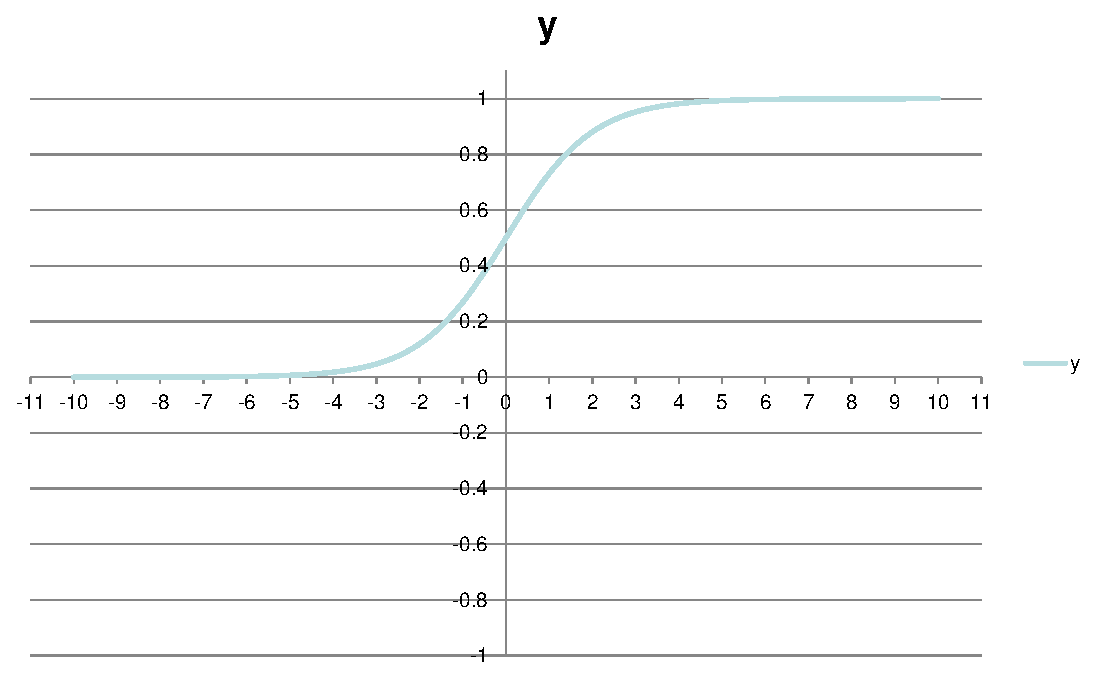
\includegraphics[width=0.3\linewidth]{logistic}}
\subfigure[tanh]{\includegraphics[width=0.3\linewidth]{tanh}}
\subfigure[relu]{\includegraphics[width=0.3\linewidth]{relu}}
\caption{Illustration of three common activate functions.}
\label{fig:mlp_activate_functions}
\end{figure}

Several neural network activation functions are plotted in Fig.~\ref{fig:mlp_activate_functions}. Their function are defined in Eq.~\ref{equ:mlp_activate_functions}.

\begin{equation}
\label{equ:mlp_activate_functions}
\begin{aligned}
{\rm{sigmoid}}\left( x \right) = \frac{1}{{1 + {e^{ - x}}}}\\
\tanh \left( x \right) &= \frac{{{e^{2x}} - 1}}{{{e^{2x}} + 1}}\\
relu\left( x \right) &= \left\{ {\begin{array}{*{20}{l}}
{x,\quad x > 0}\\
{0,\quad otherwise}
\end{array}} \right.
\end{aligned}
\end{equation}
where $logistic$ and $tanh$ are related by the following linear transform:

\begin{equation}
\label{equ:mlp_sigmoid_tanh_related}
\tanh \left( x \right) = 2sigmoid\left( {2x} \right) - 1
\end{equation}
This means that any function by a neural network with a hidden layer of tanh units can be computed by another network with logistic units and vice-versa.
They are therefore largely equivalent as activation functions.
However one reason to distinguish between them is that their output ranges are different; in particular if an output between 0 and 1 is required (for example if the output represents a probability) then the logistic sigmoid should be used.

An important feature of the three activate functions is their non-linearity. Non-linear neural networks are more powerful than linear ones since they can, for example, find non-linear classification boundaries and model non-linear equations. Moreover, any combination of linear operators is itself a linear operator, which means that any MLP with multiple linear hidden layers is exactly equivalent to some other MLP with a single linear hidden layer.
This contrast with non-linear networks, which can gain considerable power by using successive hidden layers to re-present the input data.
Their first derivatives are 

\begin{equation}
\label{equ:mlp_activate_function_logistic_derivative}
\begin{aligned}
\frac{{\partial {\rm{sigmoid}}\left( x \right)}}{{\partial x}} &= \frac{{\partial \left( {\frac{1}{{1 + {e^{ - x}}}}} \right)}}{{\partial x}}\\
 &=  - \frac{{ - {e^{ - x}}}}{{{{\left( {1 + {e^{ - x}}} \right)}^2}}}\\
 &= \frac{{{e^{ - x}}}}{{{{\left( {1 + {e^{ - x}}} \right)}^2}}}\\
 &= \frac{{{e^{ - x}}}}{{1 + {e^{ - x}}}}\frac{1}{{1 + {e^{ - x}}}}\\
 &= \frac{{1 + {e^{ - x}} - 1}}{{1 + {e^{ - x}}}}\frac{1}{{1 + {e^{ - x}}}}\\
 &= \left( {1 - {\rm{sigmoid}}\left( x \right)} \right){\rm{sigmoid}}\left( x \right)
\end{aligned}
\end{equation}

\begin{equation}
\label{equ:mlp_activate_function_tanh_derivative}
\begin{aligned}
\frac{{\partial \tanh \left( x \right)}}{{\partial x}} &= \frac{{\partial \frac{{{e^{2x}} - 1}}{{{e^{2x}} + 1}}}}{{\partial x}}\\
 &= \frac{{\partial \frac{{{e^{2x}} + 1 - 2}}{{{e^{2x}} + 1}}}}{{\partial x}}\\
 &= \frac{{\partial \left( {1 - \frac{2}{{{e^{2x}} + 1}}} \right)}}{{\partial x}}\\
 &=  - 2\frac{{\partial \left( {\frac{1}{{{e^{2x}} + 1}}} \right)}}{{\partial x}}\\
 &= 2\frac{{2{e^{2x}}}}{{{{\left( {{e^{2x}} + 1} \right)}^2}}}\\
 &= \frac{{4{e^{2x}}}}{{{{\left( {{e^{2x}} + 1} \right)}^2}}}\\
 &= \frac{{4{e^{2x}}}}{{{{\left( {{e^{2x}} + 1} \right)}^2}}} + {\left( {\frac{{{e^{2x}} - 1}}{{{e^{2x}} + 1}}} \right)^2} - {\left( {\frac{{{e^{2x}} - 1}}{{{e^{2x}} + 1}}} \right)^2}\\
 &= \frac{{4{e^{2x}} + {{\left( {{e^{2x}} - 1} \right)}^2}}}{{{{\left( {{e^{2x}} + 1} \right)}^2}}} - {\left( {\frac{{{e^{2x}} - 1}}{{{e^{2x}} + 1}}} \right)^2}\\
 &= \frac{{{{\left( {{e^{2x}} + 1} \right)}^2}}}{{{{\left( {{e^{2x}} + 1} \right)}^2}}} - {\left( {\frac{{{e^{2x}} - 1}}{{{e^{2x}} + 1}}} \right)^2}\\
 &= 1 - \tanh \left( x \right)
\end{aligned}
\end{equation}

\begin{equation}
\label{equ:mlp_activate_function_relu_derivative}
\begin{aligned}
\frac{{\partial relu\left( x \right)}}{{\partial x}} = \left\{ {\begin{array}{*{20}{l}}
{1,\quad x > 0}\\
{0,\quad otherwise}
\end{array}} \right.
\end{aligned}
\end{equation}

\begin{equation}
\label{equ:mlp_activate_function_softmax_derivative}
\begin{aligned}
\frac{{\partial {\rm{softma}}{{\rm{x}}_i}\left( x \right)}}{{\partial {x_i}}} &= \frac{{\partial \frac{{{e^{{x_i}}}}}{{\sum\limits_j {{e^{{x_j}}}} }}}}{{\partial {x_i}}}\\
 &= \frac{{{e^{{x_i}}}}}{{\sum\limits_j {{e^{{x_j}}}} }} - \frac{{{e^{{x_i}}}}}{{{{\left( {\sum\limits_j {{e^{{x_j}}}} } \right)}^2}}}\frac{{\partial \sum\limits_j {{e^{{x_j}}}} }}{{\partial {x_i}}}\\
 &= \frac{{{e^{{x_i}}}}}{{\sum\limits_j {{e^{{x_j}}}} }} - \frac{{{{\left( {{e^{{x_i}}}} \right)}^2}}}{{{{\left( {\sum\limits_j {{e^{{x_j}}}} } \right)}^2}}}\\
 &= {\rm{softma}}{{\rm{x}}_i}\left( x \right)\left( {1 - {\rm{softma}}{{\rm{x}}_i}\left( x \right)} \right)\\
 \frac{{\partial {\rm{softmax}_i}\left( x \right)}}{{\partial {x_k}}} &= \frac{{\partial \frac{{{e^{{x_i}}}}}{{\sum\limits_j {{e^{{x_j}}}} }}}}{{\partial {x_k}}}\\
 &= - \frac{{{e^{{x_i}}}}}{{{{\left( {\sum\limits_j {{e^{{x_j}}}} } \right)}^2}}}\frac{{\partial \sum\limits_j {{e^{{x_j}}}} }}{{\partial {x_k}}}\\
 &= - \frac{{ e^{x_i} e^{x_k}}}{{{{\left( {\sum\limits_j {{e^{{x_j}}}} } \right)}^2}}}\\
 &= -\rm{softmax}_{i}\left ( x \right )\rm{softmax}_k\left ( x \right )\\
\end{aligned}
\end{equation}

\section{Linear Regression}

\section{Logistic Regression}
For a binary classification problem that have two categories : $y0$ and $y1$, we want to learn a model to predict the probability of $p\left(y|x\right)$. 
Simply, we can employ a regression function to fit the probability. The most direct way is to use the linear regression function as defined by Eq.~\ref{equ:lrLinear}.

\begin{equation}
\label{equ:lrLinear}
p\left(y = y1|x\right) = {w_0x_0} + {w_1}{x_1} + {w_2}{x_2} + ... = xw
\end{equation}
where $p$ denotes the probability function, $w$ denotes the parameter vector, $x$ denotes the feature that combines the data of one dimension (value 1) corresponding to bias $w_0$. However, the value range of right part of the linear regression function falls in $\left(-\infty, \infty\right)$ while the left part need to be $\left(0, 1\right)$. To fit the value range, we scale the right part using Eq.~\ref{equ:lrScale}.

\begin{equation}
\label{equ:lrScale}
\log \frac{{p\left( {y = y1|x} \right)}}{{1 - p\left( {y = y1|x} \right)}} = xw
\end{equation}

Then $p\left( {y|x} \right)$ can be calculated by Eq.~\ref{equ:lrProbability}. Obviously, the probability function is satisfy the logistic distribution that is why we call this model logistic regression (\emph{LR}) model. In fact, the LR model assume that the data distribution between feature and category satisfy the logistic distribution, thus it can work well for linear separable data. Fig.\ref{fig:logisticRegression} shows a typical LR model.

\begin{equation}
\label{equ:lrProbability}
\begin{aligned}
p\left( {y=y1|x} \right) = \frac{1}{{1 + {e^{ - xw}}}}\\
p\left( {y=y0|x} \right) = \frac{e^{ - xw}}{{1 + {e^{ - xw}}}}
\end{aligned}
\end{equation}

The combinative form of probability function of Eq.~\ref{equ:lrProbability} can be defined by Eq.~\ref{equ:lrCombinProbability}.

\begin{equation}
\label{equ:lrCombinProbability}
\begin{aligned}
&p\left( {y|x} \right) = \left( {y = y1} \right)p\left( {y = y1|x} \right) + \left( {y = y0} \right)p\left( {y = y0|x} \right)\\
 &\quad\quad\quad= \left( {y = y1} \right)p\left( {y = y1|x} \right) + \left( {y = y0} \right)\left( {1 - p\left( {y = y1|x} \right)} \right)\\
&Let\quad y1 = 1,y0 = 0\\
 \Rightarrow &p\left( {y|x} \right) = \left( {y = 1} \right)p\left( {y = 1|x} \right) + \left( {y = 0} \right)\left( {1 - p\left( {y = 1|x} \right)} \right)\\
 &\quad\quad\quad= yp\left( {y = 1|x} \right) + \left( {1 - y} \right)\left( {1 - p\left( {y = 1|x} \right)} \right)
\end{aligned}
\end{equation}

\begin{figure}
\centering
\includegraphics[width=0.5\linewidth]{logisticRegression}
\caption{Illustration of a LR model.}
\label{fig:logisticRegression}
\end{figure}

We apply the Maximum Likelihood Estimation to estimate the parameter $w$. Since we often use loss function as our optimization object function in the supervised model, we consider the opposite number of MLE function as the loss function, as shown in Eq.~\ref{equ:lrMLE}. The optimization object shows as Eq.~\ref{equ:lrOOF}.

\begin{equation}
\label{equ:lrMLE}
{J\left( w \right)} = -p\left( {y|x} \right) = -\prod\limits_{i = 0}^{n - 1} {p\left( {{y^{*i}}|{x^{*i}}} \right)}
\end{equation}

\begin{equation}
\label{equ:lrOOF}
\mathop {J\left( w \right)}\limits_{\min }
\end{equation}

\subsection{Logarithmic Loss for Logistic Regression}
As described in Sec.\ref{sec:logFunction}, we can use log function to simplify the derivation. So the optimization object function by using logarithmic loss can be Eq.~\ref{equ:lr_loss_normal}.

\begin{equation}
\label{equ:lr_loss_normal}
\begin{aligned}
J\left( w \right) &= -\sum\limits_{i = 0}^{n - 1} {\log p\left( {{y^{*i}}|{x^{*i}}} \right)}\\
 &=  - \frac{1}{n}\sum\limits_{i = 0}^{n - 1} {\log } \left( {{y^{*i}}p\left( {{y^{*i}} = 1|{x^i}} \right) + \left( {1 - {y^{*i}}} \right)\left(1 - p\left( {{y^{*i}} = 1|{x^{*i}}} \right)\right)} \right)\\
 &=  - \frac{1}{n}\sum\limits_{i = 0}^{n - 1} \left\{{{y^{*i}}\log p\left( {{y^{*i}} = 1|{x^{*i}}} \right) + \left( {1 - {y^{*i}}} \right)\log \left(1 - p\left( {{y^{*i}} = 1|{x^{*i}}} \right) \right)}\right\} 
\end{aligned}
\end{equation}

We compute the derivation of $JS$ about the logistic output $o$ ($o = p\left( {{y} = 1|{x}}\right)$) parameter $w$ on one training sample as shown in Eq.~\ref{equ:lrDerivationOnOutput} and Eq.~\ref{equ:lrDerivation} respectively.

\begin{equation}
\label{equ:lrDerivationOnOutput}
\begin{aligned}
\frac{\partial JS}{\partial o}&=-\frac{y}{o}+\frac{1-y}{1-o}\\
&=\frac{-y+yo+o-yo}{o\times \left ( 1-o \right )}\\
&=\frac{o-y}{o\times \left ( 1-o \right )}
\end{aligned}
\end{equation}

\begin{equation}
\label{equ:lrDerivation}
\begin{aligned}
\frac{{\partial JS}}{{\partial w}} &=  - \frac{{\partial \left( {{y}\log p\left( {{y} = 1|{x}} \right) + \left( {1 - y} \right)\log \left( {1 - p\left( {{y} = 1|{x}} \right)} \right)} \right)}}{{\partial w}}\\
 &=  - \frac{{\partial \left( {y\log \left( {\frac{1}{{1 + {e^{ - xw}}}}} \right) + \left( {1 - y} \right)\log \left( {\frac{{{e^{ - xw}}}}{{1 + {e^{ - xw}}}}} \right)} \right)}}{{\partial w}}\\
 &=  - \frac{{\partial \left( {{y}\log \left( {\frac{1}{{1 + {e^{ - {x}w}}}}} \right) + \left( {1 - {y}} \right)\log \left( {\frac{{{e^{ - {x}w}}}}{{1 + {e^{ - {x}w}}}}} \right)} \right)}}{{\partial w}}\\
 &=  - \frac{{\partial \left( { - {y}\log \left( {1 + {e^{ - {x}w}}} \right) + \left( {1 - {y}} \right)\left( { - {x}w - \log \left( {1 + {e^{ - {x}w}}} \right)} \right)} \right)}}{{\partial w}}\\
 &=  - \frac{{\partial \left( { - {x}w - \log \left( {1 + {e^{ - {x}w}}} \right) + {y}{x}w} \right)}}{{\partial w}}\\
 &= \left( {1 - {y}} \right){{x} ^t} - \frac{{{e^{ - {x}w}}{{x} ^t}}}{{1 + {e^{ - {x}w}}}}\\
 &= \left( {1 - {y} - \frac{{{e^{ - {x}w}}}}{{1 + {e^{ - {x}w}}}}} \right){{x} ^t}\\
 &= \left( {p\left( {{y} = 1|{x}} \right) - {y}} \right){{x} ^t}
\end{aligned}
\end{equation}
here $x$ and $y$ indicate the feature and category for one sample respectively.

In order to determine the shape of the loss function $J$, we can compute the second order partial derivative of loss function $JS$ about $w$, as shown in Eq.~\ref{equ:lrSecondOrderDerivation}. 

\begin{equation}
\label{equ:lrSecondOrderDerivation}
\begin{aligned}
\frac{{{\partial ^2}JS}}{{\partial {w_j}\partial {w_k}}} &= {x_j}\frac{{\partial p\left( {y = 1|x} \right)}}{{\partial {w_k}}}\\
 &= \frac{{{x_j}\partial \frac{1}{{1 + {e^{ - xw}}}}}}{{\partial {w_k}}}\\
 &=  - {x_j}{\left( {1 + {e^{ - xw}}} \right)^{ - 2}}{e^{ - xw}}\left( { - {x_k}} \right)\\
 &= {x_j}{x_k}{\left( {1 + {e^{ - xw}}} \right)^{ - 2}}{e^{ - xw}}
\end{aligned}
\end{equation}

Then the Hessian matrix of $JS$ is 

\begin{displaymath}
\label{equ:lr_hessian_matrix_loss}
H = \left[ {\begin{array}{*{20}{c}}
{{x_0}^2}&{{x_0}{x_1}}&{...}&{{x_0}{x_{d - 1}}}\\
{{x_1}{x_0}}&{{x_1}^2}&{...}&{{x_1}{x_{d - 1}}}\\
{...}&{...}&{...}&{...}\\
{{x_{d - 1}}{x_0}}&{{x_{d - 1}}{x_1}}&{...}&{{x_{d - 1}}^2}
\end{array}} \right].{\left( {1 + {e^{ - xw}}} \right)^2}{e^{ - xw}}
\end{displaymath}
where $d$ indicates the dimension of the feature $x$ (including the bias).

Apparently, the matrix $H$ is real symmetrical. We can prove the loss function $JS$ is convex function through proving the real symmetrical matrix $H$ is positive semi-definite as describe in Eq.~\ref{equ:lr_half_positive_semi_definite_proof}.

\begin{equation}
\label{equ:lr_half_positive_semi_definite_proof}
\begin{aligned}
Let\ h &= \left[ {\begin{array}{*{20}{c}}
{{x_0}^2}&{{x_0}{x_1}}&{...}&{{x_0}{x_{d - 1}}}\\
{{x_1}{x_0}}&{{x_1}^2}&{...}&{{x_1}{x_{d - 1}}}\\
{...}&{...}&{...}&{...}\\
{{x_{d - 1}}{x_0}}&{{x_{d - 1}}{x_1}}&{...}&{{x_{d - 1}}^2}
\end{array}} \right]\\
given\ \alpha  &\ne Z\\
\alpha h{\alpha ^t} &= \left[ {{\alpha _0}{x_0}^2 + ... + {\alpha _{d - 1}}{x_{d - 1}}{x_0},...,{\alpha _0}{x_0}{x_{d - 1}}... + {\alpha _{d - 1}}{x_{d - 1}}^2} \right]{\alpha ^t}\\
 &= {\alpha _0}^2{x_0}^2 + {\alpha _0}{\alpha _{d - 1}}{x_{d - 1}}{x_0} + ... + {\alpha _{d - 1}}{\alpha _0}{x_0}{x_{d - 1}} + {\alpha _{d - 1}}^2{x_{d - 1}}^2\\
 &= \sum\limits_{i = 0}^{d - 1} {\sum\limits_{j = 0}^{d - 1} {{\alpha _i}{\alpha _j}{x_i}{x_j}} } \\
 &= {\left( {\sum\limits_{i = 0}^{d - 1} {{\alpha _i}{x_i}} } \right)^2} \ge 0\\
 \because \quad &{\left( {1 + {e^{ - xw}}} \right)^{ - 2}}{e^{ - xw}} > 0\\
 \Rightarrow \quad &\alpha H{\alpha ^t} \ge 0
\end{aligned}
\end{equation}

For the loss function $J$, its Hessian matrix (the result accumulating the Hessian matrices of all training samples) is still positive semi-definite thus $J$ is convex function too. 
Hence the LR model has global minimal value and may contains more than one global minimal value points.
The BSGD optimal algorithm can solve the LR model by getting the optimal solution as long as the the iteration number is enough big.
However, the Hessian matrix may be non-singular matrix, so we can not apply the Newton optimization algorithms, such as BFGS. 
To make the Hessian matrix to be a singular matrix, we can add the L-2 penalty term (L-2 penalty can restrict the complexity of the parameters which corresponds the training model).
The loss function $J$ with L-2 penalty term is defined as Eq.~\ref{equ:lr_loss_function_l2}.

\begin{equation}
\label{equ:lr_loss_function_l2}
\begin{aligned}
J\left( w \right) &=  - \frac{1}{n}\sum\limits_{i = 0}^{n - 1} {\log p\left( {{y^{*i}}|{x^{*i}}} \right)}  + \lambda \parallel w{\parallel ^2}\\
 &=  - \frac{1}{n}\sum\limits_{i = 0}^{n - 1} {\left( {\log p\left( {{y^{*i}}|{x^{*i}}} \right) + \lambda \parallel w{\parallel ^2}} \right)} 
\end{aligned}
\end{equation}

Then Eq.~\ref{equ:lrSecondOrderDerivation} can be modified by Eq.~\ref{equ:lr_second_order_derivation_l2}.

\begin{equation}
\label{equ:lr_second_order_derivation_l2}
\begin{aligned}
\frac{{{\partial ^2}JS}}{{\partial {w_j}\partial {w_k}}} &= \frac{{\partial \left( {\left( {p\left( {y = 1|x} \right) - y} \right){x_j} + 2\lambda {w_j}} \right)}}{{\partial {w_k}}}\\
 &= {x_j}\frac{{\partial p\left( {y = 1|x} \right)}}{{\partial {w_k}}} + 2\lambda \left( {j = k} \right)\\
 &= {x_j}{x_k}{\left( {1 + {e^{ - xw}}} \right)^{ - 2}}{e^{ - xw}} + 2\lambda \left( {j = k} \right)
\end{aligned}
\end{equation} 

Then the Hessian matrix of $JS$ with L-2 plenty term is 

\begin{displaymath}
\label{equ:lr_hessian_matrix_loss_l2}
H = \left[ {\begin{array}{*{20}{c}}
{{x_0}^2 + u}&{{x_0}{x_1}}&{...}&{{x_0}{x_{d - 1}}}\\
{{x_1}{x_0}}&{{x_1}^2 + u}&{...}&{{x_1}{x_{d - 1}}}\\
{...}&{...}&{...}&{...}\\
{{x_{d - 1}}{x_0}}&{{x_{d - 1}}{x_1}}&{...}&{{x_{d - 1}}^2 + u}
\end{array}} \right].{\left( {1 + {e^{ - xw}}} \right)^2}{e^{ - xw}}
\end{displaymath}
where $u = \frac{{2\lambda }}{{{{\left( {1 + {e^{ - xw}}} \right)}^2}{e^{ - xw}}}}$. We can prove the loss function $JS$ is strict convex function through proving the real symmetrical matrix $H$ is positive definite as describe in Eq.~\ref{equ:lr_positive_definite_proof}.

\begin{equation}
\label{equ:lr_positive_definite_proof}
\begin{aligned}
Let\ h & = \left[ {\begin{array}{*{20}{c}}
{{x_0}^2 + u}&{{x_0}{x_1}}&{...}&{{x_0}{x_{d - 1}}}\\
{{x_1}{x_0}}&{{x_1}^2 + u}&{...}&{{x_1}{x_{d - 1}}}\\
{...}&{...}&{...}&{...}\\
{{x_{d - 1}}{x_0}}&{{x_{d - 1}}{x_1}}&{...}&{{x_{d - 1}}^2 + u}
\end{array}} \right]\\
given\ \alpha  &\ne Z\\
\alpha h{\alpha ^t} &= \left[ {{\alpha _0}\left( {{x_0}^2 + u} \right) + ... + {\alpha _{d - 1}}{x_{d - 1}}{x_0},...,{\alpha _0}{x_0}{x_{d - 1}}... + {\alpha _{d - 1}}\left( {{x_{d - 1}}^2 + u} \right)} \right]{\alpha ^t}\\
 &= {\alpha _0}^2\left( {{x_0}^2 + u} \right) + {\alpha _0}{\alpha _{d - 1}}{x_{d - 1}}{x_0} + ... + {\alpha _{d - 1}}{\alpha _0}{x_0}{x_{d - 1}} + {\alpha _{d - 1}}^2\left( {{x_{d - 1}}^2 + u} \right)\\
 &= u\sum\limits_{i = 0}^{d - 1} {{\alpha _i}^2}  + \sum\limits_{i = 0}^{d - 1} {\sum\limits_{j = 0}^{d - 1} {{\alpha _i}{\alpha _j}{x_i}{x_j}} }  \\
 &= u\sum\limits_{i = 0}^{d - 1} {{\alpha _i}^2}  + {\left( {\sum\limits_{i = 0}^{d - 1} {{\alpha _i}{x_i}} } \right)^2} > 0\\
 \Rightarrow \alpha H{\alpha ^t} &> 0
\end{aligned}
\end{equation}

Here we get a conclusion that the loss function $J$ of logistic regression is convex and $J$ will be strictly convex when $J$ contains L-2 plenty term. In this situation, the LR model has only one global minimal value point and can apply the Newton optimal algorithms.

If we adopt the stochastic batch gradient descent algorithm, then the parameter update rule can be formalized as Eq.~\ref{equ:lrUpdateRule}.

\begin{equation}
\label{equ:lrUpdateRule}
\begin{aligned}
\Delta w &=  - \frac{1}{{nb}}\sum\limits_{i = 0}^{nb - 1} {\frac{{\partial J{S^{*i}}}}{{\partial w}}} \\
w &\leftarrow w + \Delta w
\end{aligned}
\end{equation}

\subsection{Quadratic Loss for Logistic Regression}

\begin{displaymath}
J\left ( w \right ) = \frac{1}{2} \sum_{N-1}^{i = 0} \left ( p\left ( y=1|x \right ) - y \right ) ^ 2
\end{displaymath}

\begin{displaymath}
\frac{\partial JS}{\partial o} = p\left ( y=1|x \right ) - y
\end{displaymath}

\begin{displaymath}
\begin{aligned}
\frac{\partial JS}{\partial w}&={p}{'}\left ( y=1|x \right )\left ( p\left ( y=1|x \right ) - y \right )x\\
&=p\left ( y=1|x \right )\left ( 1 - p\left ( y=1|x \right ) \right )\left ( p\left ( y=1|x \right ) - y \right )x^t
\end{aligned}
\end{displaymath}

We can see that when $p\left ( y=1|x \right )$ is close to $1$ or $0$, the derivative value of $JS$ about $w$ will be close to $0$. If $p\left ( y=1|x \right )$ and $y$ are all close to $1$ or $0$, quadratic loss will not brings obstruction for learning. Otherwise, $p\left ( y=1|x \right )$ near to $1$ or $0$ will reduce the learning speed.

\section{Softmax}
We can exploit LR model to acquire the probability function for binary categories. How can we extend the LR to more categories? In this section we will introduce the softmax model to handle the multi-class classification.

Similar to LR model, we want to acquire the probability of each category for a given sample. So we adopt the vector to encode the categories. For example, if the number of categories is 3, we use $\left[1, 0, 0\right]$ denotes the first category, $\left[0, 1, 0\right]$ and $\left[0, 0, 1\right]$ denote the second and third category respectively.

The key for generating the probability of multiple categories is to define the probability function which scale the linear regression function to probability function. In LR model, we exploit the log function for the ratio between $p$ and $1 - p$ to matching the value range of linear regression function. Here, we can not use the same way to calculate probability due to the insoluble function group as shown in Eq.~\ref{equ:softmaxInsoluble}.

\begin{equation}
\label{equ:softmaxInsoluble}
\left\{ {\begin{array}{*{20}{c}}
{\log \frac{{{p}\left( {y_i = 1|x} \right)}}{{1 - {p}\left( {y_i = 1|x} \right)}} = x{w_{\_i}}}\\
{\sum\limits_{i = 0}^{{\hat d} - 1} {{p}\left( {y_i = 1|x} \right) = 1} }
\end{array}} \right.
\end{equation} 
here $\hat d$ denotes the dimension of output while $d$ denotes the dimension of the input feature, $x$ denote the input feature of one sample and $y$ denotes the output vector encoded in binary type.

We exploit other way to compute the probability as shown in Eq.~\ref{equ:softmaxProbability}. 

\begin{equation}
\label{equ:softmaxProbability}
\begin{aligned}
&{p}\left( {y_i = 1|x} \right) = f\left( {x{w_{\_i}}} \right) > 0\\
 &\to {p}\left( {y_i = 1|x} \right) = {e^{x{w_{\_i}}}} \in \left( {0,1} \right)\\
 &\to {p}\left( {y_i = 1|x} \right) = \frac{{{e^{x{w_{\_i}}}}}}{{\sum\limits_{j = 0}^{d - 1} {{e^{x{w_{\_j}}}}} }} = {\rm{softma}}{{\rm{x}}_i}\left( {x,w} \right)
\end{aligned}
\end{equation}

Similar to LR model, the optimization object function can be Eq.~\ref{equ:softmaxOOF}.

\begin{equation}
\label{equ:softmaxOOF}
\begin{aligned}
J\left( w \right) &=  - \frac{1}{n}\sum\limits_{i = 0}^{n - 1} {\log p\left( {{y^{*i}}|{x^{*i}}} \right)} \\
 &=  - \frac{1}{n}\sum\limits_{i = 0}^{n - 1} {\log \sum\limits_{j = 0}^{\hat d - 1} {\left( {{y^{*i}}_j = 1} \right){p\left( {{y_j}^{*i} = 1|{x^{*i}}} \right)}}}\\
 &=  - \frac{1}{n}\sum\limits_{i = 0}^{n - 1} {\sum\limits_{j = 0}^{\hat d - 1} {\left( {{y_j}^{*i} = 1} \right)} \log p\left( {{y_j}^{*i} = 1|{x^{*i}}} \right)}\\
 &=  - \frac{1}{n}\sum\limits_{i = 0}^{n - 1} {\sum\limits_{j = 0}^{\hat d - 1} {\left( {{y_j}^{*i} = 1} \right)} \log \frac{{{e^{x*{w_{\_j}}}}}}{{\sum\limits_{k = 0}^{\hat d - 1} {{e^{x*{w_{\_k}}}}} }}}
\end{aligned}
\end{equation}
Note that Softmax regression has an unusual property that it has a "redundant" set of parameters. To explain what this means, suppose we take each of our parameter vectors $w_j$, and subtract some fixed vector $\psi$ from it, so that every $w_j$ is now replaced with $w_j - \psi$, then we have 

\begin{displaymath}
\begin{aligned}
\log \frac{{{e^{x{w_{\_j}}}}}}{{\sum\limits_{k = 0}^{\hat d - 1} {{e^{x{w_{\_k}}}}} }}&=\log \frac{{{e^{x\left ( {w_{\_j}-\psi} \right )}}}}{{\sum\limits_{k = 0}^{\hat d - 1} {{e^{x\left ( {w_{\_k}-\psi} \right )}}} }}\\
&=\log \frac{{{e^{x\psi}e^{x\left ( {w_{\_j}-\psi} \right )}}}}{{\sum\limits_{k = 0}^{\hat d - 1} {{e^{x\psi}e^{x\left ( {w_{\_k}-\psi} \right )}}} }}\\
&=\log \frac{{{e^{x{w_{\_j}}}}}}{{\sum\limits_{k = 0}^{\hat d - 1} {{e^{x{w_{\_k}}}}} }}
\end{aligned}
\end{displaymath}
Hence, the optimal solution is not unique.
If we force the $\psi = w_0$, then we will have 

\begin{displaymath}
\begin{aligned}
\log \frac{{{e^{x{w_{\_j}}}}}}{{\sum\limits_{k = 0}^{\hat d - 1} {{e^{x{w_{\_k}}}}} }}&=\log \frac{{{e^{x\left ( {w_{\_j}-w_{\_0}} \right )}}}}{{\sum\limits_{k = 0}^{\hat d - 1} {{e^{x\left ( {w_{\_k}-w_{\_0}} \right )}}} }}\\
Let\ \tilde{w}_{\_j} &= w_{\_j} - w_{\_0}\\
\Rightarrow \tilde{w}_{\_0} &= \vec{0}\\
\tilde{w}_{\_1} &= w_{\_1} - w_{\_0}\\
\tilde{w}_{\_2} &= w_{\_2} - w_{\_0}\\
\end{aligned}
\end{displaymath}
So we can always force one vector of weight (i.e. $w_{\_0} = \vec{0}$), this will reduce the number of learning parameters. 
In practice, however, it is often cleaner and simpler to implement the version which keeps all the parameters $w_{\_0}, w_{\_1}...$, without arbitrarily setting one of them to zero. But we will make one change to the cost function: Adding penalty term such as L-2 term. This will take care of the numerical problems associated with softmax regression's overparameterized representation. 

The derivation of $JS$ about the softmax output $o_j$ ($o_j = \rm{softmax}_j\left(x\right)$), $w_j$ and $w$ on one training sample can be computed as Eq.~\ref{equ:softmaxDerivationOnOutput}, Eq.~\ref{equ:softmaxDerivationOnW_p} and Eq.~\ref{equ:softmaxDerivationOnW} respectively.

\begin{equation}
\label{equ:softmaxDerivationOnOutput}
\begin{aligned}
\frac{\partial JS}{\partial o_j}=\left ( y_j = 1 \right )\frac{-1}{o_j}
\end{aligned}
\end{equation}

\begin{equation}
\label{equ:softmaxDerivationOnW_p}
\begin{aligned}
\frac{{\partial JS}}{{\partial {w_{\_j}}}} &=  - \frac{{\partial \sum\limits_{k = 0}^{\hat d - 1} {{y_k}\log \frac{{{e^{x{w_{\_k}}}}}}{{\sum\limits_{l = 0}^{\hat d - 1} {{e^{x{w_{\_l}}}}} }}} }}{{\partial {w_{\_j}}}}\\
 &= \frac{{\partial \sum\limits_{k = 0}^{\hat d - 1} {{y_k}\left( {\log \sum\limits_{l = 0}^{\hat d - 1} {{e^{x{w_{\_l}}}}}  - x{w_{\_k}}} \right)} }}{{\partial {w_{\_j}}}}\\
 &= \sum\limits_{k = 0}^{\hat d - 1} {{y_k}} \frac{{\partial \left( {\log \sum\limits_{l = 0}^{\hat d - 1} {{e^{x{w_{\_l}}}}}  - x{w_{\_k}}} \right)}}{{\partial {w_{\_j}}}}\\
 &= \sum\limits_{k = 0}^{\hat d - 1} {{y_k}} \frac{{\partial \left( {\log \sum\limits_{l = 0}^{\hat d - 1} {{e^{x{w_{\_l}}}}}  - x{w_{\_k}}} \right)}}{{\partial {w_{\_j}}}}\\
 &= \frac{{\partial \log \sum\limits_{l = 0}^{\hat d - 1} {{e^{x{w_{\_l}}}}} }}{{\partial {w_{\_j}}}} - \frac{{\sum\limits_{k = 0}^{\hat d - 1} {{y_k}x{w_{\_k}}} }}{{\partial {w_{\_j}}}}\\
 &= \frac{1}{{\sum\limits_{k = 0}^{\hat d - 1} {{e^{x{w_{\_k}}}}} }}\frac{{\partial \sum\limits_{k = 0}^{\hat d - 1} {{e^{x{w_{\_k}}}}} }}{{\partial {w_{\_j}}}} - {y_j}{x^t}\\
 &= \frac{{{e^{x{w_{\_j}}}}}}{{\sum\limits_{k = 0}^{\hat d - 1} {{e^{x{w_{\_k}}}}} }}{x^t} - {y_j}{x^t}\\
 &= \left( {\frac{{{e^{x{w_{\_j}}}}}}{{\sum\limits_{k = 0}^{\hat d - 1} {{e^{x{w_{\_k}}}}} }} - {y_j}} \right){x^t}\\
 &= \left( {{\rm{softma}}{{\rm{x}}_j}\left( {x,w} \right) - {y_j}} \right){x^t}\\
 &= {\delta _j}\left( x \right){x^t}
\end{aligned}
\end{equation}

\begin{equation}
\label{equ:softmaxDerivationOnW}
\begin{aligned}
\frac{{\partial J\left( w \right)}}{{\partial w}} &= \left[ {\frac{{\partial J\left( w \right)}}{{\partial {w_{\_0}}}},\frac{{\partial J\left( w \right)}}{{\partial {w_{\_1}}}},...} \right]\\
 &= \left[ {{\delta _0}\left( x \right){x^t},{\delta _1}\left( x \right){x^t},...} \right]\\
 &= {x^t}\left[ {{\delta _0}\left( x \right),{\delta _1}\left( x \right),...} \right]\\
 &= {x^t}\left( {{\rm{softmax}}\left( {x,w} \right) - y} \right)
\end{aligned}
\end{equation}

In order to determine the shape of the loss function $J$, we can compute the second order partial derivative of loss function $JS$ about $w$, as shown in Eq.~\ref{equ:softmax_second_derivative}. 

The Hessian matrix of the loss function $JS$ is 

We can find that the Hessian matrix is is a positive semi-definite and non-singular matrix. Hence the softmax model is also a convex optimization problem that has the global minimal value but has many global minimal value points.
Besides, softmax model can not apply the Newton optimization algorithm.
Similar to the LR model, we can add the L-2 penalty term to make the Hessian matrix to be a positive definite and singular matrix. Thus the loss function is strict convex function, and the softmax model will has only one global minimal value point and can apply the Newton optimization algorithm.

Here we don't discuss the update rule of parameters since it is similar to LR model. The softmax regression can be consider as the extension of LR model due to the similar in two aspects. Specifically, in one hand, the probability functions are similar as shown in Eq.~\ref{equ:softmaxSimilarPF}. In the other hand, the loss function in LR model can be written like softmax model as shown in Eq.~\ref{equ:softmaxSimilarLoss}

\begin{equation}
\label{equ:softmaxSimilarPF}
{\rm{softma}}{{\rm{x}}_i}\left( {x,w} \right) = \frac{{{e^{x{w_{\_i}}}}}}{{\sum\limits_{j = 0}^{d - 1} {{e^{x{w_{\_j}}}}} }} = \frac{1}{{1 + \sum\limits_{j \ne i} {{e^{x\left( {{w_{\_j}} - {w_{\_i}}} \right)}}} }}
\end{equation}

\begin{equation}
\label{equ:softmaxSimilarLoss}
\begin{aligned}
J\left( w \right) =  - \frac{1}{n}\sum\limits_{i = 0}^{n - 1} {\left\{ {{y^{*i}}\log p\left( {{y^{*i}} = 1|{x^i}} \right) + \left( {1 - {y^{*i}}} \right)\log \left( {1 - p\left( {{y^{*i}} = 1|{x^i}} \right)} \right)} \right\}} \\
 =  - \frac{1}{n}\sum\limits_{i = 0}^{n - 1} {\sum\limits_{j = 0}^{d - 1} {\left( {{y_j}^{*i} = 1} \right)} \log p\left( {{y_j}^{*i} = 1|{x^{*i}}} \right)} 
\end{aligned}
\end{equation}

\section{MLP}
\label{sec:mlp}
Artificial neural networks (ANNs) were originally developed as mathematical models of the information processing capabilities of biological brains\footnote{This section refers to the paper of \cite{Graves_RNN_2012}.}.
Although it is now clear that ANNs bear little resemblance to real biological neurons, they enjoy continuing popularity as pattern classifiers.

The basic structure of an ANN is a network of small processing units, or nodes, joined to each other by weighted connections.
In terms of the original biological model, the nodes represent neurons, and the connection weights represent the strength of the synapses between the neurons.
The network is activated by providing an input to some or all of the nodes, and this activation then spreads throughout the network along the weighted connections.
The electrical activity of biological neurons typically follows a series of sharp 'spikes', and the activation of an ANN node was originally intended to model the average firing rate of these spikes.

Many varieties of ANNs have appeared over the years, with widely varying properties.
One important distinction is between ANNs whose connections form cycles, and those whose connection are acyclic.
ANNs with cycles are referred to as feedback, recursive or recurrent, neural networks and are dealt with in Sec.~\ref{sec:rnn}.
Anns without cycles are referred to as feed-forward neural networks (FNNs). Well known examples of FNNs include \emph{perceptrons} \cite{Rosenblatt_Perceptron_1958}, \emph{radial basis function networks} \cite{Broomhead_Radial_NN_1988}, Kohonen maps and Hopfield nets.
The most widely used form of FNN, and the one we focus on in this section, is the multilayer perceptron (MLP), \cite{Rumelhart_BP_1986, Werbos_BP_1990}, learned by Back Propagation (BP).
As shown in Fig.\ref{fig:bpNeuralNetwork}, the units in a MLP are arranged in layers, with connections feeding forward from one layer to the next.
Input patterns are presented to the input layer $o^{*0}$, the propagated through the hidden layer $o^{*1}$ to the output layer $o^{*2}$. This process is known as the \emph{forward pass} of the network.

\begin{figure}
\centering
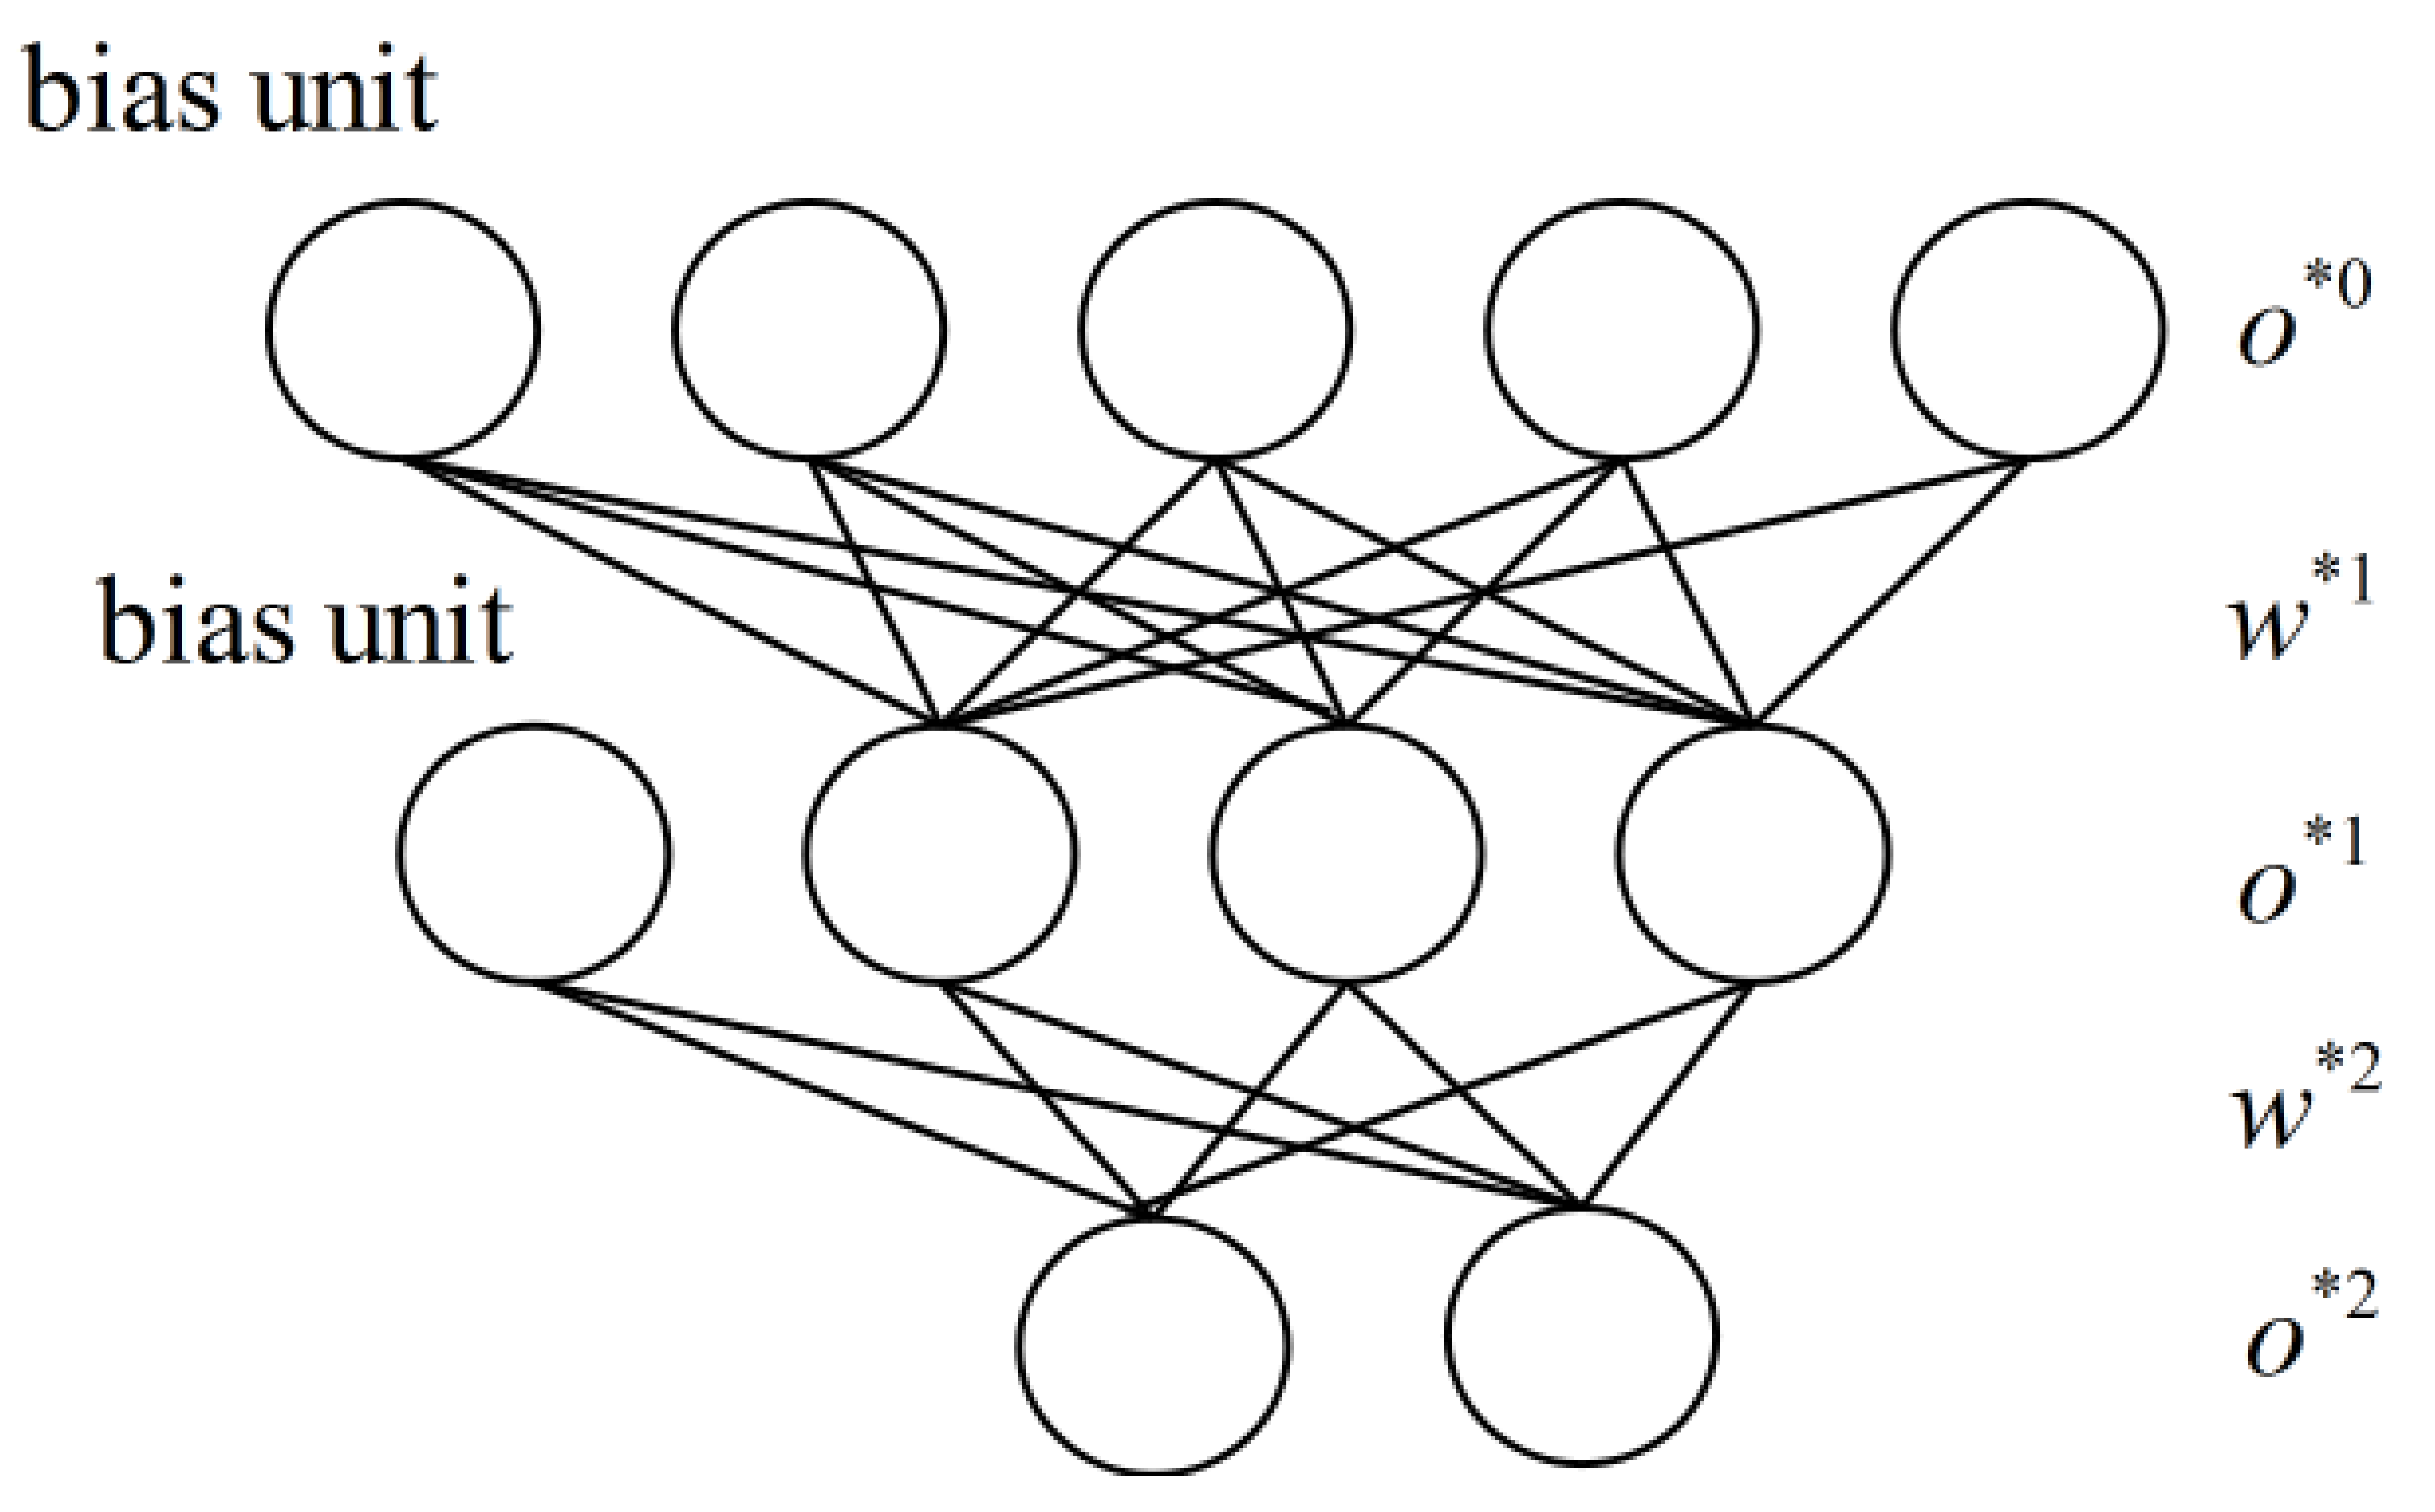
\includegraphics[width=0.5\linewidth]{bpNeuralNetwork}
\caption{Illustration of Back Propagation Neural Network.}
\label{fig:bpNeuralNetwork}
\end{figure}
where $o^{*0}, o^{*1}, o^{*2}$ denote the input layer, hidden layer and output layer, respectively.

Since the output of an MLP depends only on the current input, and not on any past or future inputs, MLPs are more suitable for pattern classification than for sequence labelling. We will discuss this point further in Sec.~\ref{sec:rnn}.

An MLP with a particular set of weight values defines a function from input to output vectors.
By altering the weights, a single MLP is capable of instantiating many different functions.
Indeed it has been proven \cite{Hornik_Universal_Function_1989} that an MLP with a single hidden layer containing a sufficient number of non-linear units can approximate any continuous function on a compact input domain to arbitrary precision.
For this reason MLPs are said to be \emph{universal function approximators}.

\subsection{Forward Pass}
Consider an MLP with some layers (the first one is the input layer while the last is output layer), each unit in the layer calculates a weighted sum of the units of previous layer. We refer the weighted sum as $s^{*l}$.
The activation function $f$ is then applied, yielding the final activation $o^{*l}$. 
We first discuss the output in hidden layers.
Denoting the weight from unit $i$ to unit $j$ as $w_{ij}$, the bias of unit $j$ as $b_{j}$, we have

\begin{equation}
\label{equ:mlp_forward_output}
\begin{aligned}
{s_j}^{*l} = \sum\limits_i {{w^{*l}}_{ij}{o^{*l - 1}}_i}  + {b_j}\\
{o^{*l}} &= f\left( {{s_j}^{*l}} \right)
\end{aligned}
\end{equation}

The output layer can be considered appending a layer of linear regression, or logistic regression, or soft-max model after the last hidden layer of the MLP.
The type of activate function on output layer depends on the specific task. For regression tasks, we use linear function or logistic function. While for classification tasks, we employ logistic function or soft-max function. 

\subsection{Back Propagation}
Let $J$ denotes the loss function (optimization object function), $JS$ denotes the loss function in one sample, $w$ denotes the weight between two layers (includes bias), $n$ denotes the count of training samples, $nb$ denotes the batch size, we adopt the stochastic batch descent algorithm, then we have Eq.~\ref{equ:bpOOF}.

\begin{equation}
\label{equ:bpOOF}
\begin{aligned}
\mathop {\min }\limits_w J &= \mathop {\min }\limits_w \frac{1}{n}\sum\limits_{i = 0}^{n - 1} {J{S^{*i}}}\\
&\approx \frac{1}{{nb}}\sum\limits_{i = 0}^{nb - 1} {J{S^{*i}}}\\
\end{aligned}
\end{equation}

We first calculate derivative of loss function on one sample. 
Let $d^{*i}$ denotes the dimension in $ith$ layer. $s$ denotes the linear output of layer, $o$ denotes the activation function value of layer ($o^{*0}$ denotes the $n * d^{*0}$ input feature), $loss$ denotes loss vector, the $y$ denotes the $n * d^{*last}$ category, , $f$ denotes the activation or output function.
For a back propagation neural work, we have the base Eq.~\ref{equ:bpBaseEqu}.

\begin{equation}
\label{equ:bpBaseEqu}
\begin{aligned}
{s^{*l + 1}} &= {o^{*l}}{w^{*l + 1}} + {b^{*l + 1}}\\
{o^{*l}} &= f\left( {{s^{*l}}} \right)\\
{o^{*last}} &= f\left( {f\left( {f\left( {{o^{*0}}{w^{*1}} + {b^{*1}}} \right){w^{*2}} + {b^{*2}}} \right)...{w^{*last}} + {b^{*last}}} \right)\\
los{s_j} &= JSD\left( {{o^{*last}}_j,{y_j}} \right)\\
JS &= \sum\limits_j {los{s_j}} 
\end{aligned}
\end{equation}

As we can see that the loss function is a function 

The calculation of partial derivative of $JS$ about $w$ shows as Eq.~\ref{equ:bpGD}.
\begin{equation}
\label{equ:bpGD}
\begin{aligned}
\frac{\partial{JS}}{\partial{w^{*l}_{ij}}} &= \frac{\partial{JS}}{\partial{s^{*l}_{j}}}\frac{\partial{s^{*l}_{j}}}{\partial{w^{*l}_{ij}}}\\
&= \frac{\partial{JS}}{\partial{o^{*l}_{j}}}\frac{\partial{o^{*l}_{j}}}{\partial{s^{*l}_{j}}}\frac{\partial{s^{*l}_{j}}}{\partial{w^{*l}_{ij}}}\\
&= \sum_{k}{\frac{\partial{JS}}{\partial{s^{*l + 1}_{k}}}\frac{{\partial{s^{*l + 1}_{k}}}}{\partial{o^{*l}_{j}}}}\frac{\partial{o^{*l}_{j}}}{\partial{s^{*l}_{j}}}\frac{\partial{s^{*l}_{j}}}{\partial{w^{*l}_{ij}}},l < last\\
\end{aligned}
\end{equation}

\begin{equation}
\frac{\partial{s^{*l}_{j}}}{\partial{w^{*l}_{ij}}} = o^{*l-1}_{i}
\end{equation}
\begin{equation}
\delta^{*l}_{j} = \frac{\partial{JS}}{\partial{s^{*l}_{j}}} = \left\{
\begin{aligned}
\sum_{k}{\delta^{*l + 1}_{k}w^{*l + 1}_{jk}}f^{'}(s^{*l}_{j}), l < last\\
\frac{\partial{loss_{j}}}{\partial{o^{*last}_{j}}}f^{'}(s^{*last}_{j}), l = last\\
\end{aligned}
\right.
\end{equation}

\begin{equation}
\frac{\partial{JS}}{\partial{w^{*l}_{ij}}} = \delta^{*l}_{j}o^{*l - 1}_{i}
\end{equation}

\begin{equation}
\delta^{*l} = \left\{
\begin{aligned}
\delta^{*l + 1}(w^{*l + 1})^{t}f^{'}(s^{*l}), l < last\\
\frac{\partial{loss}}{\partial{o^{*l}}}f^{'}(s^{*l}), l = last\\
\end{aligned}
\right.
\end{equation}

\begin{equation}
\begin{aligned}
\frac{\partial{JS}}{\partial{w^{*l}}} &= 
\begin{bmatrix}
\delta^{*l}_{0}o^{*l - 1}_{0}& ... & \delta^{*l}_{n - 1}o^{*l - 1}_{0} \\
... & ... & ... \\
\delta^{*l}_{0}o^{*l - 1}_{m - 1} & ... & \delta^{*l}_{n - 1}o^{*l - 1}_{m - 1}
\end{bmatrix}\\
&= (o^{*l - 1})^{t}\delta^{*l}\\
\end{aligned}
\end{equation}

The calculation of partial derivative of $JS$ about $b$ shows as Eq.~\ref{equ:bp_derivative_bias}.

\begin{equation}
\label{equ:bp_derivative_bias}
\begin{aligned}
\frac{{\partial JS}}{{\partial {b^{*l}}_j}} &= \frac{{\partial JS}}{{\partial {s^{*l}}_j}}\frac{{\partial {s^{*l}}_j}}{{\partial {b^{*l}}_j}}\\
 &= \frac{{\partial JS}}{{\partial {s^{*l}}_j}}\frac{{\partial {s^{*l}}_j}}{{\partial {b^{*l}}_j}}\\
 &= {\delta ^{*l}}_j\\
 \Rightarrow \frac{{\partial JS}}{{\partial {b^{*l}}}} &= {\delta ^{*l}}
\end{aligned}
\end{equation}

If $o$ and $\delta$ are all denote $nb$ rows matrix (that is to say, $o$ and $\delta$ are calculated on batch training samples), the update rule is shown as Eq.~\ref{equ:bpWeightUpdateRule}.

\begin{equation}
\label{equ:bpWeightUpdateRule}
\begin{aligned}
\frac{{\partial J}}{{\partial {w^{*l}}}} &\approx \frac{1}{{nb}}\sum\limits_{i = 0}^{nb - 1} {\frac{{\partial J{S^{*i}}}}{{\partial {w^{*l}}}}} \\
 &= \frac{1}{{nb}}\sum\limits_{i = 0}^{nb - 1} {{{\left( {{o_{i\_}}^{*l - 1}} \right)}^t}{\delta _{i\_}}^{*l}} \\
 &= \frac{1}{{nb}}{\left( {{o^{*l - 1}}} \right)^t}{\delta ^{*l}}\\
\frac{{\partial J}}{{\partial {b^{*l}}}} &\approx \frac{1}{{nb}}\sum\limits_{i = 0}^{nb - 1} {\frac{{\partial J{S^{*i}}}}{{\partial {b^{*l}}}}} \\
&= \frac{1}{{nb}}\sum\limits_{i = 0}^{nb - 1} {{\delta ^{*l}}_{i\_}}\\
\Delta w^{*l} &=  - \frac{{\partial J}}{{\partial {w^{*l}}}}\\
\Delta {b^{*l}} &=  - \frac{{\partial J}}{{\partial {b^{*l}}}}\\
w^{*l} &\leftarrow w^{*l} + \Delta w^{*l}\\
b^{*l} &\leftarrow b^{*l} + \Delta b^{*l}
\end{aligned}
\end{equation}

\subsection{Derivative Tricks}
For DR curve based models, the basic structure can be divided into two categories as shown in Fig.~\ref{fig:dr_model_structure_type}.

\begin{figure}
\centering
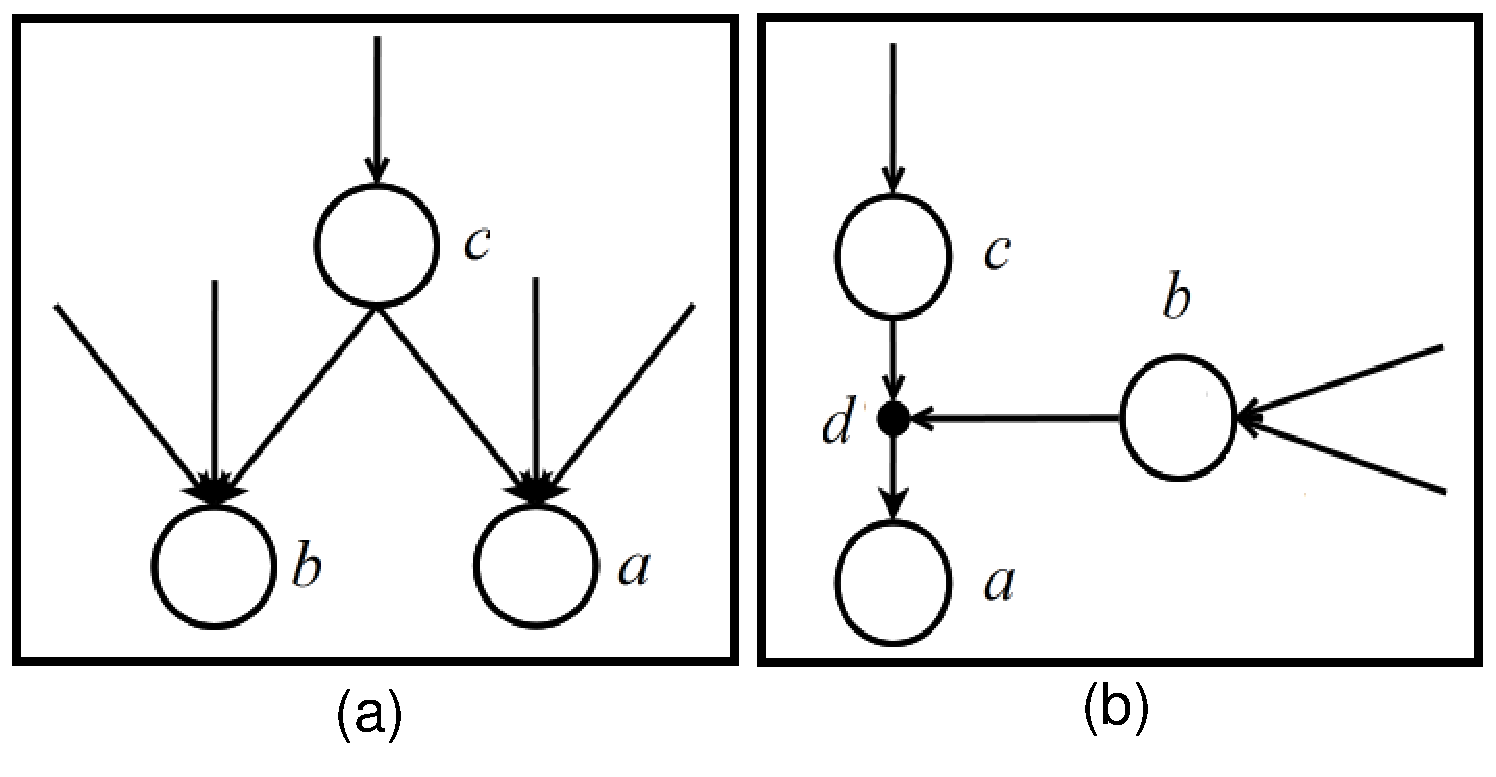
\includegraphics[width=0.7\linewidth]{dr_model_structure_type}
\caption{Two categories of basic structure of DR curve models. Where the weight from $c$ to $d$ and from $b$ to $d$ is constant weight of value $1$.}
\label{fig:dr_model_structure_type}
\end{figure}

For the type shown in Fig.~\ref{fig:dr_model_structure_type} (a), we have Eq.~\ref{equ:dr_type_a_loss}. While for Fig.~\ref{fig:dr_model_structure_type} (b), we have Eq.~\ref{equ:dr_type_b_loss}.

\begin{equation}
\label{equ:dr_type_a_loss}
\begin{aligned}
loss &= f\left( {{s_{*a}},{s_{*b}}} \right)\\
 \Rightarrow {\delta _{*c}} &= \frac{{\partial loss}}{{\partial {s_{*c}}}} = \frac{{\partial loss}}{{\partial {s_{*a}}}}\frac{{\partial {s_{*a}}}}{{\partial {s_{*c}}}} + \frac{{\partial loss}}{{\partial {s_{*b}}}}\frac{{\partial {s_{*b}}}}{{\partial {s_{*c}}}}\\
 &= {\delta _{*a}}\frac{{\partial \left( {{o_{*c}}{w_{*c\_to\_a}}} \right)}}{{\partial {o_{*c}}}}\frac{{\partial {o_{*c}}}}{{\partial {s_{*c}}}} + {\delta _{*b}}\frac{{\partial \left( {{o_{*c}}{w_{*c\_to\_b}}} \right)}}{{\partial {o_{*c}}}}\frac{{\partial {o_{*c}}}}{{\partial {s_{*c}}}}\\
 &= {f^{'}}\left( {{s_{*c}}} \right)\left( {{\delta _{*a}}{w_{*c\_to\_a}} + {\delta _{*b}}{w_{*c\_to\_b}}} \right)
\end{aligned}
\end{equation}

\begin{equation}
\label{equ:dr_type_b_loss}
\begin{aligned}
loss &= f\left( {{s_{*a}}} \right)\\
 \Rightarrow {\delta _{*c}} &= \frac{{\partial loss}}{{\partial {s_{*a}}}}\frac{{\partial {s_{*a}}}}{{\partial {o_{*c}}}}\frac{{\partial {o_{*c}}}}{{\partial {s_{*c}}}}\\
 &= {\delta _{*a}}\frac{{\partial \left( {{o_{*b}}{o_{*c}}{w_{*d\_to\_a}}} \right)}}{{\partial {o_{*c}}}}{f^{'}}\left( {{s_{*c}}} \right)\\
 &= {\delta _{*a}}{w_{*d\_to\_a}}{o_{*b}}{f^{'}}\left( {{s_{*c}}} \right)\\
{\delta _{*b}} &= \frac{{\partial loss}}{{\partial {s_{*a}}}}\frac{{\partial {s_{*a}}}}{{\partial {o_{*b}}}}\frac{{\partial {o_{*b}}}}{{\partial {s_{*b}}}}\\
 &= {\delta _{*a}}\frac{{\partial \left( {{o_{*b}}{o_{*c}}{w_{*d\_to\_a}}} \right)}}{{\partial {o_{*b}}}}{f^{'}}\left( {{s_{*b}}} \right)\\
 &= {\delta _{*a}}{w_{*d\_to\_a}}{o_{*c}}{f^{'}}\left( {{s_{*b}}} \right)
\end{aligned}
\end{equation}


\section{MLPs Problems}

\subsection{Over-fitting}
\label{sec:overFittingInDR}
Suppose that we have a perfect training data (\emph{normalized data}) that can reflect the real data distribution without any noise in a practical problem and be learned successfully by machine learning model. That is to say, all of the training data can be correctly classified in classification problem or accurately fitted in regression problem. The learned model is the best model we need (even though it is in over-fitting training), as shown in Fig.\ref{fig:overFittingOnPerfectData}. Usually, the learning model should be very complex that the number of learned parameters is more than the dimension of feature of training data. We use the DR curve to describe the learning result from a machine learning model. What the discriminant/regressive curve looks like? Most possibly, the DR curve is very smooth due to the DR boundary of the training data distribution should be naturally smooth in feature space. Such DR curve is our supreme learning object, we call it supreme DR curve.

When we use complex model train the imperfect training data, the insufficient training data or noise may makes the shape of the supreme DR curve in-smooth so that the DR curve may diverge from the supreme DR curve.
Specifically, in the situation of imperfect training data, the wrong category noise data may obviously bring some sharp point to DR curve or even generate discontinuous DR curve. Besides, the large interval in feature space may lightly affect the trend of DR curve. In additional, the wrong feature noise data may affect the trend of DR curve when there miss some training data in the path between wrong feature space and the correct space, as shown in Fig.\ref{fig:overFittingWrongDiscriminantCurve}. As we can see, only the missed training data near the discriminant curve will bring negative influence to DR curve.

\begin{figure}
\centering
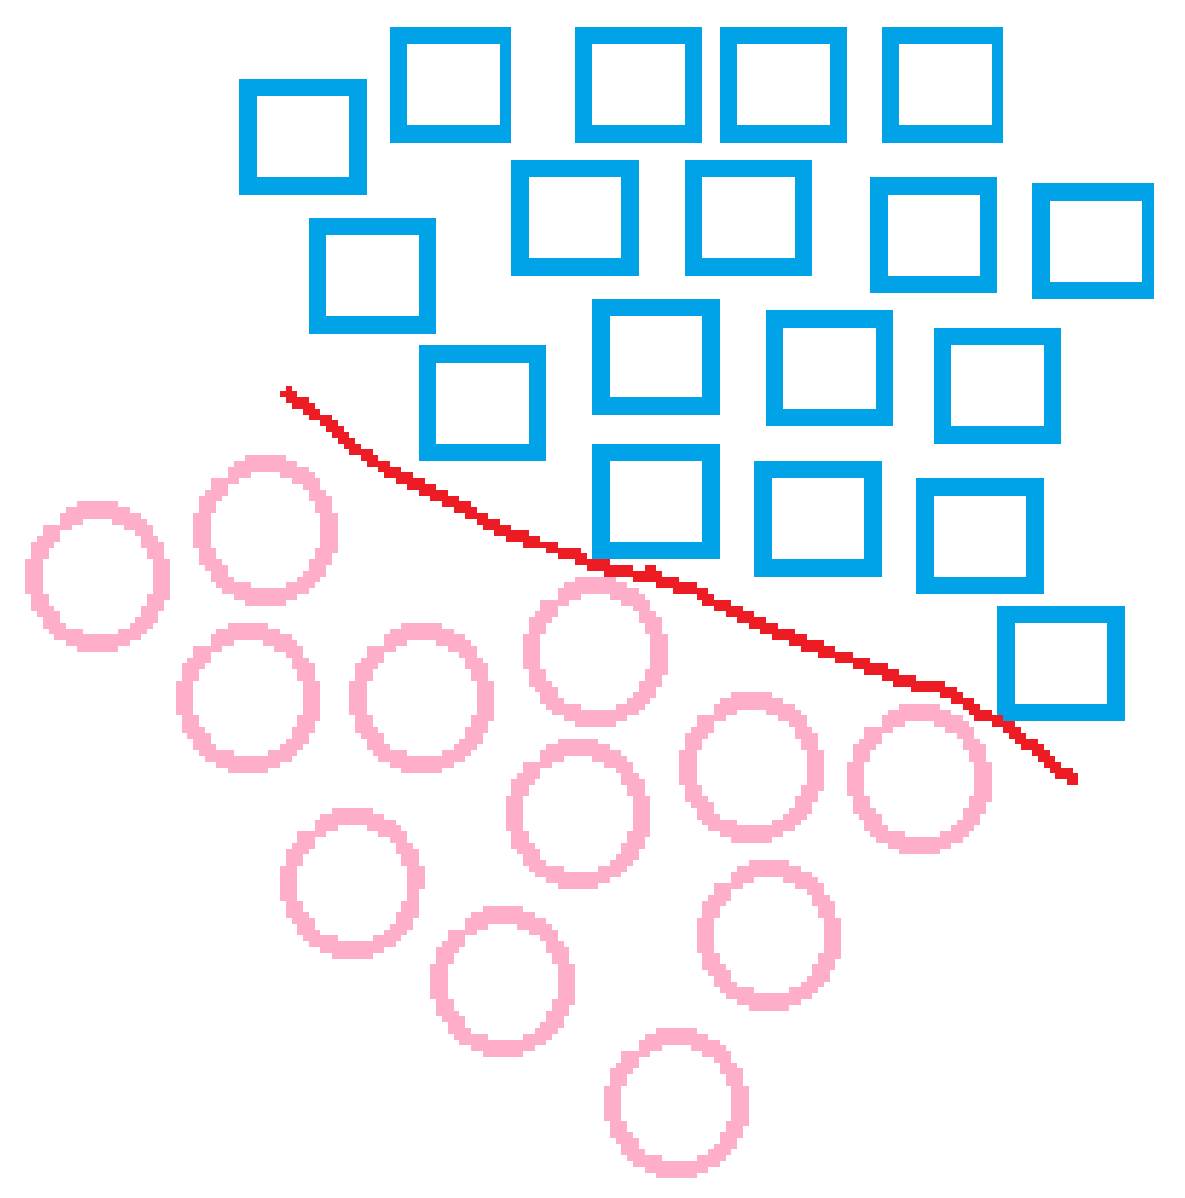
\includegraphics[width=0.35\linewidth]{overFittingOnPerfectData}
\caption{Illustration of the discriminant curve in over-fitting situation in perfect training data.}
\label{fig:overFittingOnPerfectData}
\end{figure}

\begin{figure}
\centering
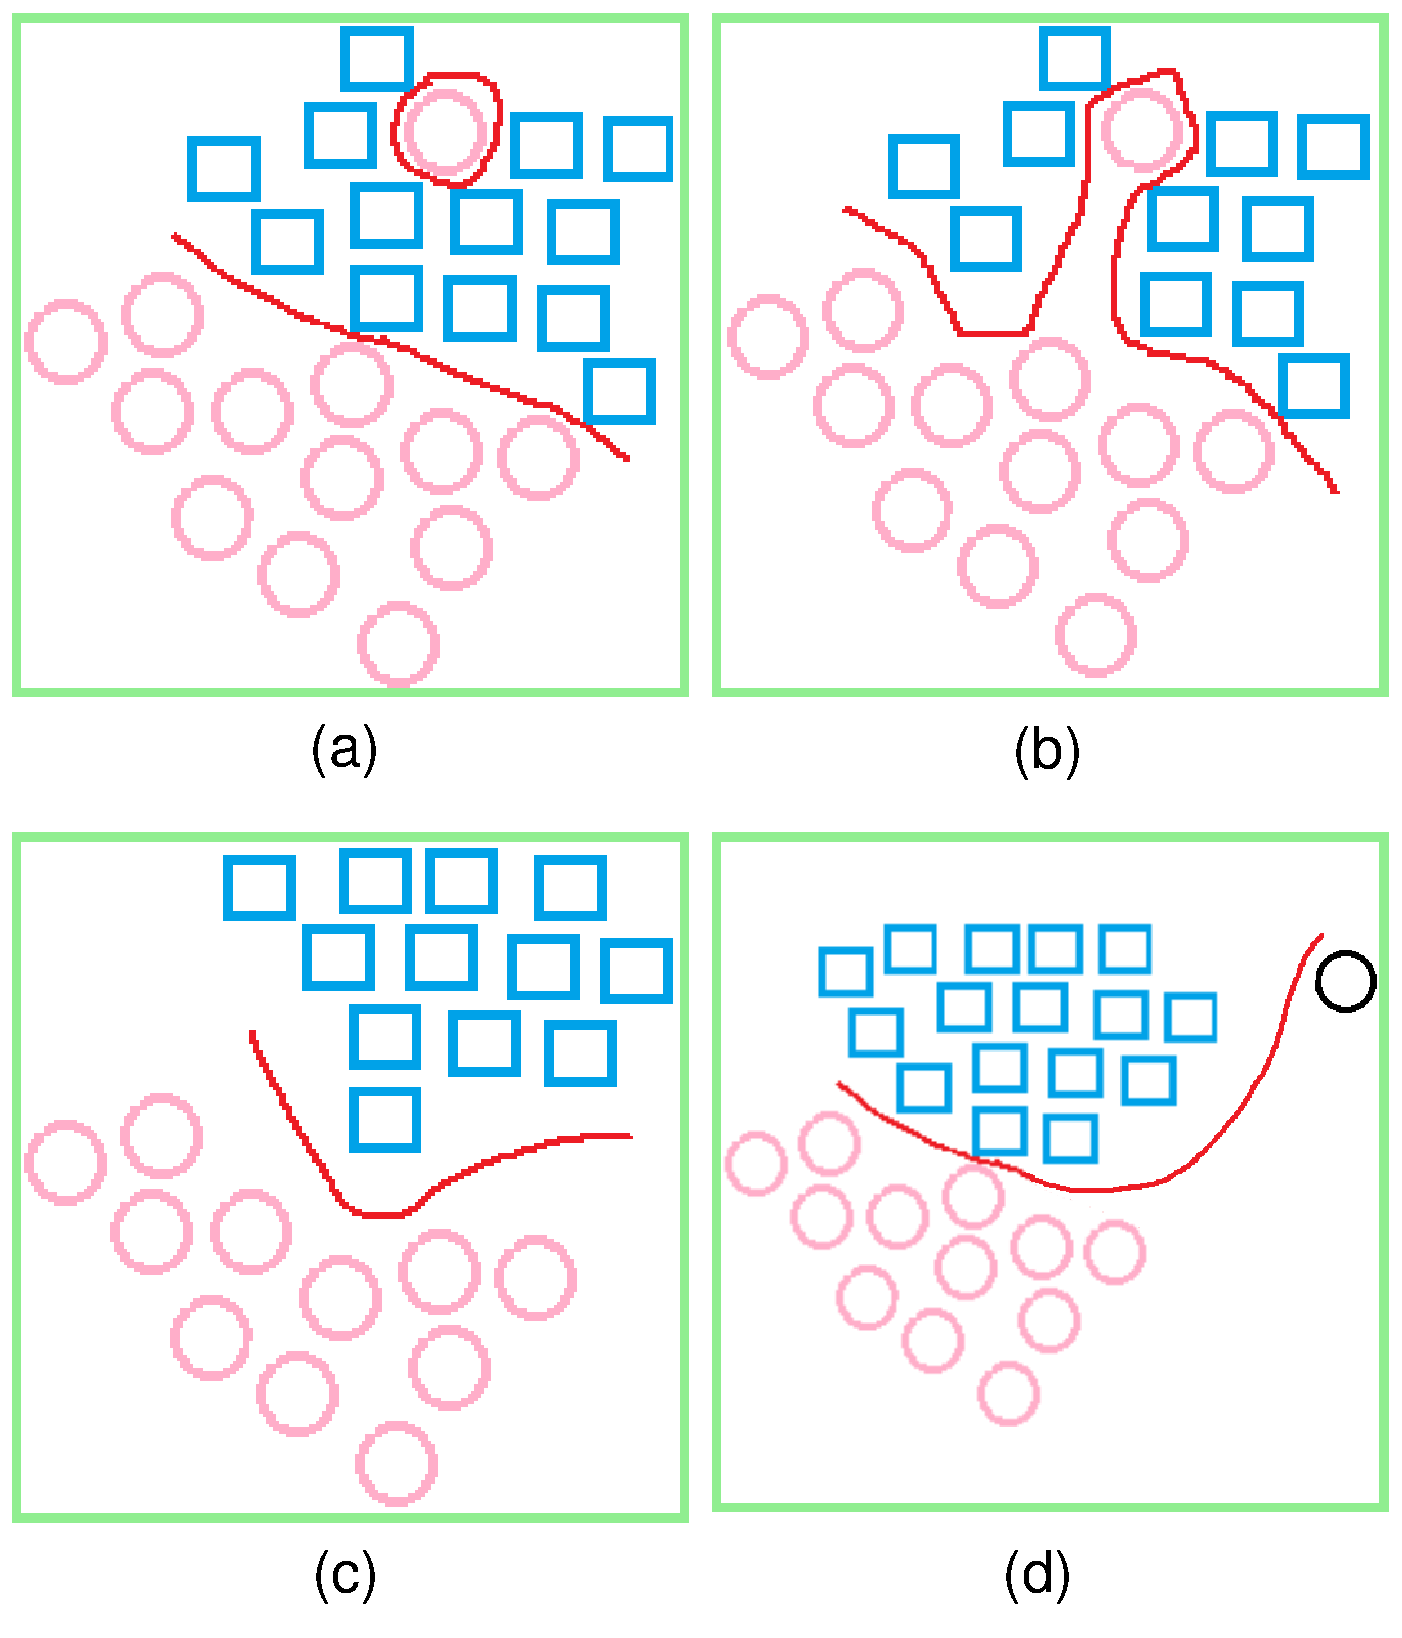
\includegraphics[width=1.0\linewidth]{overFittingWrongDiscriminantCurve}
\caption{Illustration of the discriminant curve in over-fitting situation in whole and noisy and insufficient training data. (a) shows the discontinuous DR curve since the noise data locating in the accumulation area of different category. (b) shows the sharp point generated by the noise data. (c) shows the incorrect trend of discriminant curve affected by the lack of training data. (d) shows the incorrect trend of discriminant curve affected by the lack of training data in the path between wrong feature space and the correct space.}
\label{fig:overFittingWrongDiscriminantCurve}
\end{figure}

If we want to learn a supreme DR curve, we need a very complex model. 
However, if the model is too complex, the real learned DR curve is different from supreme DR curve when the training data is imperfect.
The practicable way to handle the dilemma, we need to restrict the complexity of the learning model.
A direct way is to reduce the number of parameters. However, reducing the parameters number will reduce the learning capacity. 
In most times, we adopt a strategy to restrict the complexity of models while keep the scale of the parameters considerable.
DR curve based models transform the feature from original feature space to a new feature space through non-linear transformation, an function example of DR curve with two features is shown in Eq.~\ref{equ:overFittingDRFunctionHighOrder}. 

\begin{equation}
\label{equ:overFittingDRFunctionHighOrder}
g\left( {\theta, x} \right) = {\theta_0} + {\theta_1}{x_0} + {\theta_2}{x_1} + {\theta_3}{x_0}{x_1} + {\theta_4}{x_0}^2 + {\theta_5}{x_1}^2 + {\theta_6}{x_0}^2{x_1}
\end{equation}
Where the $\theta$ is the parameters of the model and $x$ is a 2 dimensions feature. ${x_0}{x_1}$, ${x_0}^2$, ${x_1}^2$ and ${x_0}^2{x_1}$ can be considered the new features learned from the DR curve based model. 

In the over-fitting situation, the DR curve has many sharp point so that the function of DR curve is very complex. Thus the non-linear transformation is very complex. 
For example, in multilayer perceptron, the output of layers can be computed by Eq.~\ref{equ:overFittingMLPOutput}.

\begin{equation}
\label{equ:overFittingMLPOutput}
\begin{aligned}
{\left( {{o^{*last}}} \right)_j} &= \sum {{{\left( {{w^{*last}}} \right)}_{ij}}{{\left( {{o^{*last - 1}}} \right)}_i}} \\
...\\
{\left( {{o^{*1}}} \right)_j} &= \sum {{{\left( {{w^{*1}}} \right)}_{ij}}{{\left( {{o^{*0}}} \right)}_i}} 
\end{aligned}
\end{equation}
Where $weight$ denotes the weight. We ignore the bias term.
A complex non-linear transformation means the $o^{*last}_{j}$ is very complex. Hence the diversity of ${{{\left( {{w^{*last}}} \right)}_{ij}}{{\left( {{o^{*last - 1}}} \right)}_i}}$ is very striking ($w^{*last}$ is in the wide range) and every term ${{{\left( {{o^{*l - 1}}} \right)}_i}}$ is complex.
As a recursive result, all weights should be in wide range.
Thus to make the DR curve more smooth, the direct way is to restrict the value of learned parameters (assume parameters satisfy some distributions, such as L1 and L2 regularizations, see in Sec.~\ref{sec:penalty_term}). 
Here the restrict is on the learned parameters, not the initial learning parameters.
Though we usually use Gaussian method to initialize the learning parameters, the setting of Gaussian of learning parameter is under the assumption of the diversity of importances of different dimensions of input feature (see details in Sec.~\ref{sec:mlp_normlize_inputs} and \ref{sec:mlp_learning_parameter_initialization}).

Notice that, for the linear regression, logistic regression and softmax models, the L2 regularization is just want to restrict the parameters in a centralized range under the assumption of the importance of different dimensions of feature should satisfy Gaussian distribution that majority dimensions of feature can be treated impartially.

\subsection{Hard Parameters Setting}

\subsection{Low Learning Speed}

\subsection{Forward Signal Explosion}

\subsection{Gradient Explosion and Decay}
\label{sec:mlp_gradient_explosion_dacay}
As shown in Eq.~\ref{equ:bpGD}, ${{\delta ^{*l}}_{{k^{*l}}}}$ can be written a function with variable ${{\delta ^{*l + t}}_{{k^{*l + t}}}}$, hence we can calculate the derivative of $\frac{{\partial {\delta ^{*l}}_{{k^{*l}}}}}{{\partial {\delta ^{*l + t}}_{{k^{*l + t}}}}}$ as Eq.~\ref{equ:mlp_delta_recursion}.

\begin{equation}
\label{equ:mlp_delta_recursion}
\begin{aligned}
\frac{{\partial {\delta ^{*l}}_{{k^{*l}}}}}{{\partial {\delta ^{*l + 1}}_{{k^{*l + 1}}}}} &= {w^{*l + 1}}_{{k^{*l}}{k^{*l + 1}}}{f^{'}}\left( {{s^{*l}}_{{k^{*l}}}} \right)\\
\frac{{\partial {\delta ^{*l}}_{{k^{*l}}}}}{{\partial {\delta ^{*l + 2}}_{{k^{*l + 2}}}}} &= \sum\limits_{{k^{*l + 1}}} {{w^{*l + 1}}_{{k^{*l}}{k^{*l + 1}}}{f^{'}}\left( {{s_{{k^{*l}}}}^{*l}} \right){w^{*l + 2}}_{{k^{*l + 1}}{k^{*l + 2}}}{f^{'}}\left( {{s^{*l + 1}}_{{k^{*l + 1}}}} \right)} \\
\frac{{\partial {\delta ^{*l}}_{{k^{*l}}}}}{{\partial {\delta ^{*l + t}}_{{k^{*l + t}}}}} &= \sum\limits_{{k^{*l + 1}}} {\frac{{\partial {\delta ^{*l}}_{{k^{*l}}}}}{{\partial {\delta ^{*l + 1}}_{{k^{*l + 1}}}}}\sum\limits_{{k^{*l + 2}}} {\frac{{\partial {\delta ^{*l + 1}}_{{k^{*l + 1}}}}}{{\partial {\delta ^{*l + 2}}_{{k^{*l + 2}}}}}...\frac{{\partial {\delta ^{*l + t - 1}}_{{k^{*l + t - 1}}}}}{{\partial {\delta _k}^{*l + t}}}} } \\
 &= \sum\limits_{{k^{*l + 1}}} {{w^{*l + 1}}_{{k^{*l}}{k^{*l + 1}}}{f^{'}}\left( {{s^{*l}}_{{k^{*l}}}} \right)\sum\limits_{{k^{*l + 2}}} \begin{array}{l}
{w^{*l + 2}}_{{k^{*l + 1}}{k^{*l + 2}}}{f^{'}}\left( {{s^{*l + 1}}_{{k^{*l + 1}}}} \right)\\
...{w^{*l + t}}_{{k^{*l + t - 1}}{k^{*l + t}}}{f^{'}}\left( {{s^{*l + t - 1}}_{{k^{*l + t - 1}}}} \right)
\end{array} } \\
 &= \sum\limits_{{k^{*l + 1}}} {...\sum\limits_{{k^{*l + t - 1}}} {\prod\limits_{\hat l = l + 1}^{l + t} {{w^{*\hat l}}_{{k^{*\hat l - 1}}{k^{*\hat l}}}{f^{'}}\left( {{s^{*\hat l - 1}}_{{k^{*\hat l - 1}}}} \right)} } } 
\end{aligned}
\end{equation}

As Eq.~\ref{equ:mlp_delta_recursion} shown, the total error back flow (note that since the summation terms may have different signs, increasing the number of units does not necessarily increase error flow due to the multiplication operation is more important than summation).

If 

\begin{displaymath}
|{{w^{*\hat l}}_{{k^{*\hat l - 1}}{k^{*\hat l}}}{f^{'}}\left( {{s^{*\hat l - 1}}_{{k^{*\hat l - 1}}}} \right)}| > 1.0
\end{displaymath}

for all units (as can happen, e.g., with linear activate function or large weight) then the largest product increases exponentially with $t$. That is, the error blows up and conflicting error arriving at unit $v$ can lead to oscillating weights and unstable learning (too large absolute value of weights). If

\begin{displaymath}
|{{w^{*\hat l}}_{{k^{*\hat l - 1}}{k^{*\hat l}}}{f^{'}}\left( {{s^{*\hat l - 1}}_{{k^{*\hat l - 1}}}} \right)}| < 1.0
\end{displaymath}

then the largest product decrease exponentially with $t$. That is, the gradient vanishes, and nothing can be learned in acceptable time. Note that in the training stages with gradient descent algorithm, the gradient vanishes are more possible to occur, since the sum of different very large value with different signs may be small, while the sum of different very small value with different signs is small too.

If activate function $f\left( s \right)$ is the logistic sigmoid function, we have

\begin{equation}
\label{equ:mlp_vanish_logistic_vanish}
\begin{aligned}
&{w^{*\hat l}}_{{k^{*\hat l - 1}}{k^{*\hat l}}}{f^{'}}\left( {{s^{*\hat l - 1}}_{{k^{*\hat l - 1}}}} \right)\\
 =& {w^{*\hat l}}_{{k^{*\hat l - 1}}{k^{*\hat l}}}f\left( {{s^{*\hat l - 1}}_{{k^{*\hat l - 1}}}} \right)\left( {1 - f\left( {{s^{*\hat l - 1}}_{{k^{*\hat l - 1}}}} \right)} \right)\\
 =& \frac{{{w^{*\hat l}}_{{k^{*\hat l - 1}}{k^{*\hat l}}}\exp \left( {\sum\limits_{{k^{*\hat l - 2}}} {{w^{*\hat l - 1}}_{{k^{*\hat l - 2}}{k^{*\hat l - 1}}}f\left( {{s^{*\hat l - 2}}_{{k^{*\hat l - 2}}}} \right)}  + {b^{*\hat l - 1}}_{{k^{*\hat l - 1}}}} \right)}}{{{{\left( {1 + \exp \left( {\sum\limits_{{k^{*\hat l - 2}}} {{w^{*\hat l - 1}}_{{k^{*\hat l - 2}}{k^{*\hat l - 1}}}f\left( {{s^{*\hat l - 2}}_{{k^{*\hat l - 2}}}} \right)}  + {b^{*\hat l - 1}}_{{k^{*\hat l - 1}}}} \right)} \right)}^2}}}\\
 \approx &\frac{{{w^{*\hat l}}_{{k^{*\hat l - 1}}{k^{*\hat l}}}\exp \left( { - \sum\limits_{{k^{*\hat l - 2}}} {{w^{*\hat l - 1}}_{{k^{*\hat l - 2}}{k^{*\hat l - 1}}}f\left( {{s^{*\hat l - 2}}_{{k^{*\hat l - 2}}}} \right)} } \right)}}{{{{\left( {1 + \exp \left( { - \sum\limits_{{k^{*\hat l - 2}}} {{w^{*\hat l - 1}}_{{k^{*\hat l - 2}}{k^{*\hat l - 1}}}f\left( {{s^{*\hat l - 2}}_{{k^{*\hat l - 2}}}} \right)} } \right)} \right)}^2}}}\\
=& \frac{{{w^{*\hat l}}_{{k^{*\hat l - 1}}{k^{*\hat l}}}}}{{1 + \exp \left( { - \sum\limits_{{k^{*\hat l - 2}}} {{w^{*\hat l - 1}}_{{k^{*\hat l - 2}}{k^{*\hat l - 1}}}f\left( {{s^{*\hat l - 2}}_{{k^{*\hat l - 2}}}} \right)} } \right)}}\frac{1}{{1 + \exp \left( {\sum\limits_{{k^{*\hat l - 2}}} {{w^{*\hat l - 1}}_{{k^{*\hat l - 2}}{k^{*\hat l - 1}}}f\left( {{s^{*\hat l - 2}}_{{k^{*\hat l - 2}}}} \right)} } \right)}}
\end{aligned}
\end{equation}
it's maximal value goes to zero when $|w| \to  + \infty $ (assume all the $|w|$ are approximate, then ${f}\left( s \right) \to 1\ or\ 0$, so ${f^{'}}\left( s\right) \to 0$), and is less than $1.0$ for $|{w^{*\hat l}}_{{k^{*\hat l}}{k^{*\hat l + 1}}}| < 4.0$.
Hence with conventional logistic sigmoid activate functions, the error flow tends to vanish as long as the weights have absolute values below 4.0, especially in the beginning of the training phase.
In general the use of large initial weights will not help though - as seen above, for $|w| \to  + \infty $ the relevant derivative goes to zero "faster" than the absolute weight can grow (also, some weights will have to change their signs by crossing zero).
Likewise, increasing the learning rate does not help either - it will not change the ratio of long-range error flow.

Usually we initialize the weight and bias with the value in range of $(0, 1)$, this will reduce the probability of gradient explosion problem (in fact gradient explosion is low possible so that it is not the main problem). 
For gradient decay problem, we can adopt two strategies: employ different learning rate in different layers and adopt the approximate linear activate function with high derivative.
For the strategy of different learning rate, we can use large learning rate in the initial layers while the small learning rate in latter layers. However, when the layer is too deep, then the propagation error in initial layers will be closed to or is zero that the strategy will be failed.
For the strategy of approximate linear activate function, we can employ relu or maxout activate function due to their derivative is similar to $1$. 

\section{Tricks for MLPs}

\subsection{Normalizing the Inputs}
\label{sec:mlp_normlize_inputs}
Convergence is usually faster if \emph{the average of each input variable over the training set is close to zero}.
To see this, consider the extreme case where all the inputs are positive. 
Weights to a particular unit denotes ${w_{\_j}}$ (the connections between the units in previous data layer to the next data layer unit $j$) in the first weight layer are updated by an amount proportional  to $o\delta$ where $o$ is the input vector and $delta$ is the scalar error at the unit.
When all of the components of an input vector are positive, all of the updates of weights that feed into a unit will be the same sign (i.e. sign($\delta$)).
As a result, these weights can only all decrease or all increase \emph{together} for a given input pattern.
Thus, if $w_{\_j}$ must change direction it can only do so by zigzagging which is inefficient and thus very slow (the batch learning can reduce the zigzagging situation by smoothing the update direction).

In the above example, the inputs were all positive. However, in general, if the data in each dimension are mostly positive or negative, the weights are still update in a particular direction and thus slow down learning.
Therefore, it is good to shift the inputs so that the average over the training set is close to zero.
This heuristic should be applied at all layers which means that we want to average of the outputs of a unit to be close to zero becasue these outputs are the inputs of the next layer.
This problem can be addressed by coordinating how the inputs are transformed with the choice of sigmoid activation (using tanh instead of sigmoid function due to the value range of sigmoid function is in $\left(0, 1\right)$ while for tanh is $\left(-1, 1\right)$).

Usually, \emph{the input data are considered to be comparably important for the learning problem, that is the feature in different dimensions should have the same range of value}. 
Hence we often to scale the covariances of the input data to the same value (usually $1$ for the convenience of parameter setting in different learning problems using the similar configuration learning algorithm).

As we know, the initial weights are often drawn from Gaussian distribution (this mean the value of weights is centralized) under the assumption of the DR curve of DR based model is smooth when the different dimensions of input data are normalized to the same scale, as described in Sec.~\ref{sec:overFittingInDR}.
Convergence is faster not only if the inputs are shifted as described above but also if they are scaled so that all have about the same covariance.
If the input data is not scaled, then the output maybe solely depends on the part of the input data with large absolute value. The contributions of different dimensions of input data are not comparable.
To fit the loss function, the DR based model trend to sharply adjust the weight to let ${{{\left( {{o^{*l}}} \right)}_{\hat i}}{w_{\hat ij}}}$ to be comparable.
This may takes a lot of times. 
Hence, scaling speeds learning because it helps to balance out the rate at which the weights connected to the input nodes learn.
In other word, all dimensions contribute obviously to the learning.

The exception to scaling all covariances to the different value occurs when it is know that some inputs are of less significance than others.
In such a case, it can be beneficial to scale the less significant inputs down so that they are "less visible" to the learning process.

The above two tricks of shifting and scaling the inputs are quite simple to implement.
Another trick that is quite effective but more difficult to implement is to decorrelate the inputs.
Consider the simple network in Fig.~\ref{fig:normalizing_input_decorrelated}.
If inputs are uncorrelated then it is possible to solve for the value of $w_{0}$ that minimizes the error without any concern for $w_{1}$, and vice versa.
In other words, the two variables are independent.
With correlated inputs, one must solve for both simultaneously which is much harder problem.
Principal component analysis can be used to remove linear correlations in inputs.

Inputs that are linearly dependent (the extreme case of correlation) may also produce degeneracies which may slow learning.
Consider the case where one input $x_{1}$ is always twice the other input $x_{0}$. The network output $y$ will take the form from ${x_0}{w_0} + {x_1}{w_1} + b$ to ${x_0}\left( {{w_0} + 2{w_1}} \right) + b$.
We can use a new weight ${\tilde w}$ to replace $w_0$ and $w_1$, then the output is ${x_0} {\tilde w} + b$.
If we have other input units such as $x_2$, $x_3$ and so on, the $x_0$ will be more important to the DR based model when the initial weights are comparable.

\begin{figure}
\centering
\includegraphics[width=0.5\linewidth]{normalizing_input_decorrelated}
\caption{Linear dependent inputs.}
\label{fig:normalizing_input_decorrelated}
\end{figure}

Fig.~\ref{fig:normalizing_input_processing} shows the entire process of normalizing inputs for DR based models. The steps are (1) shift inputs so the mean is zero, (2) decorrelate inputs, (3)equalize convariances.

\begin{figure}
\centering
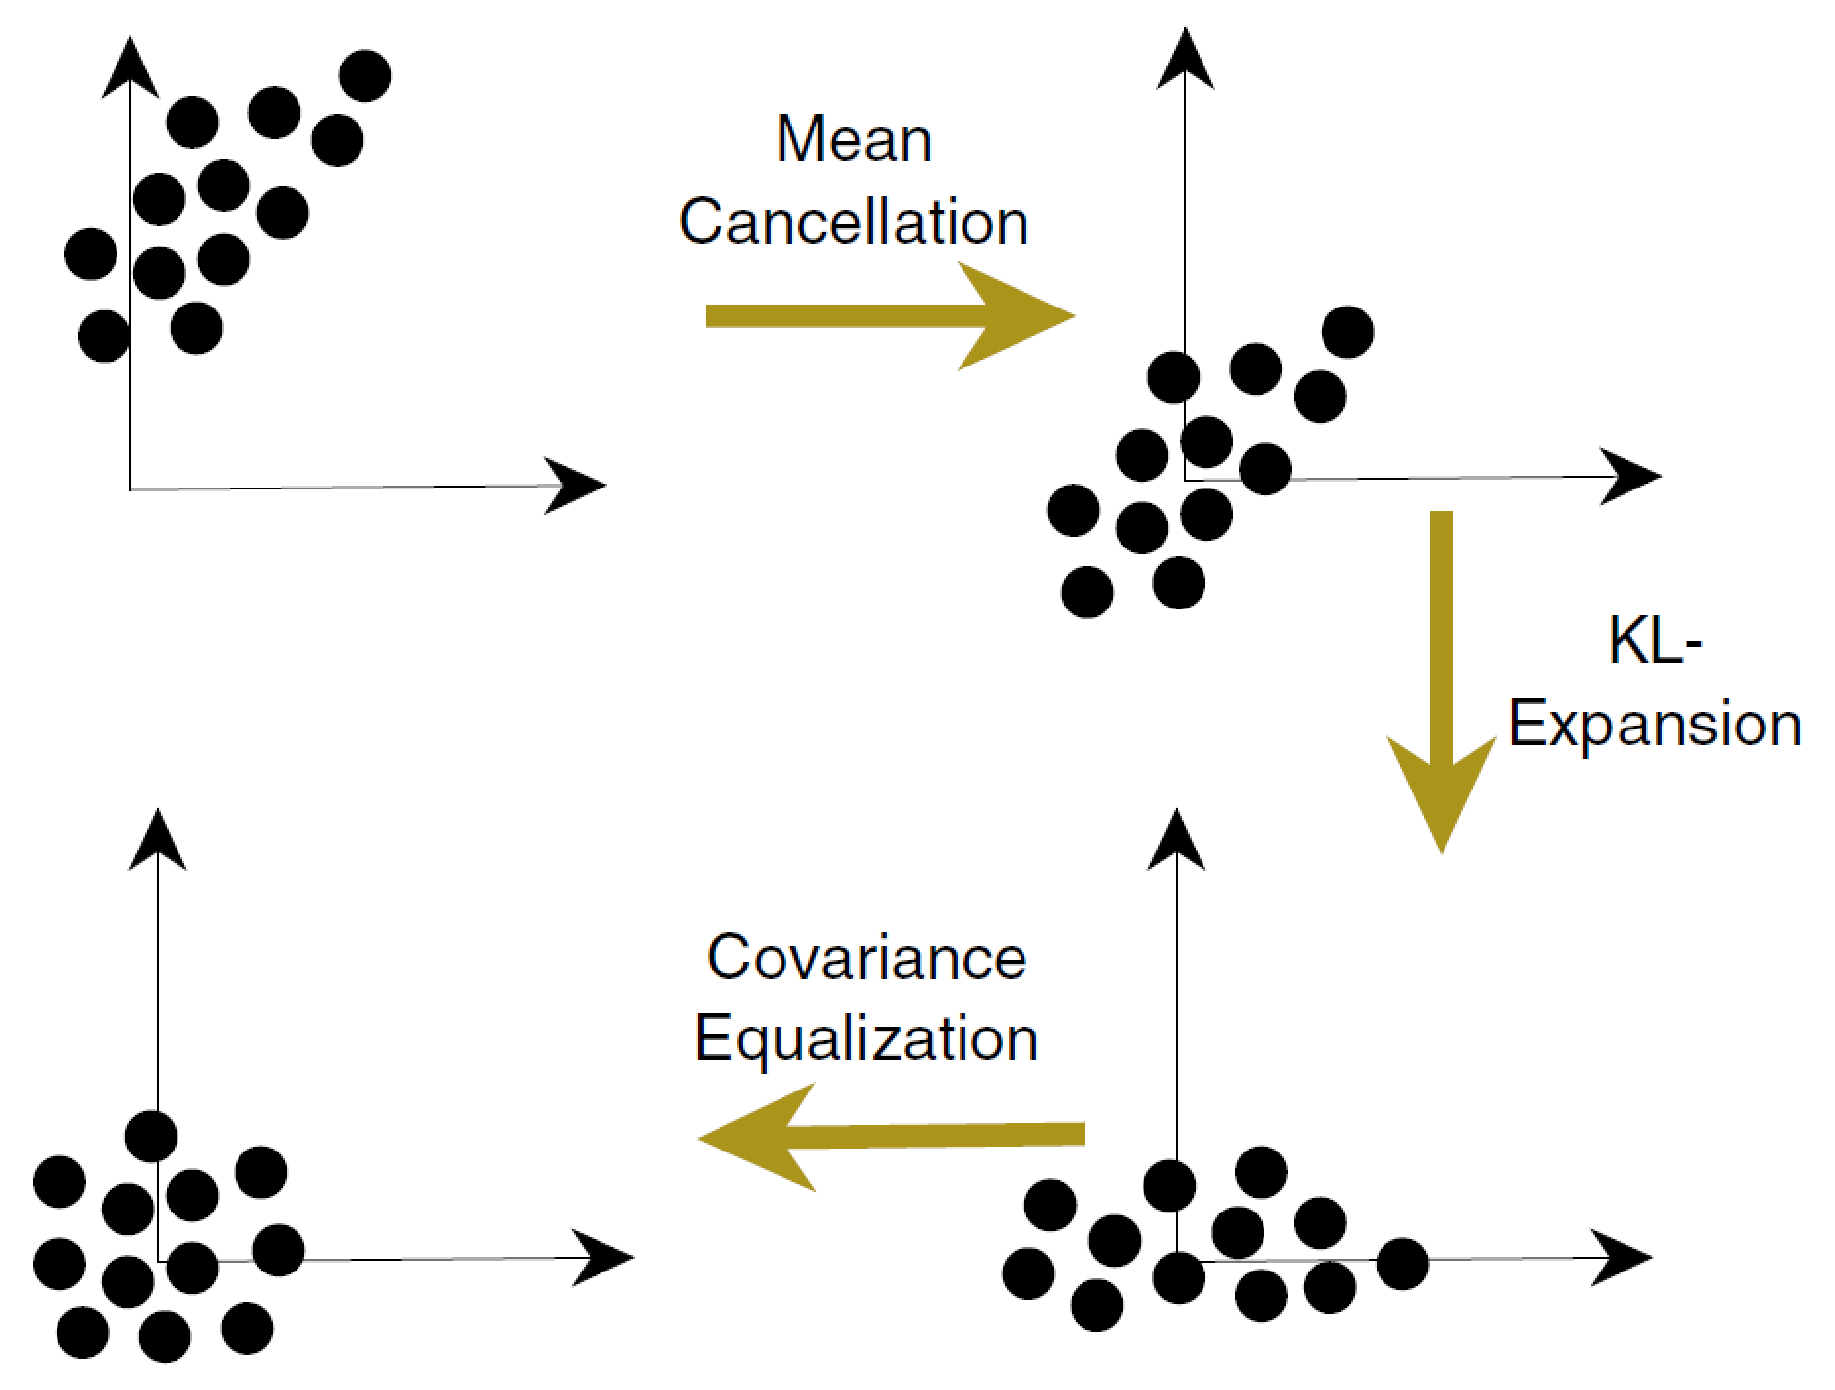
\includegraphics[width=0.5\linewidth]{normalizing_input_processing}
\caption{Normalizing inputs.}
\label{fig:normalizing_input_processing}
\end{figure}

\subsection{Learning Parameters and Rate Initialization}
\label{sec:mlp_learning_parameter_initialization}
The learning parameters consist of two parts: weights and biases.
The biases can be consider the special weights that the input activate values are contant $1$.
The initialization of learning rate need to reference to the weights.
If the variance of learning parameters is big, then the learning rate should be big too, and vice-versa.
The small learning rate in optimization algorithm trend to have low update of gradient, which can be ignored for comparing with the big variance of weights (there are many big weights if the variance are big).

Under the assumption of the input data are considered to be comparably important for the learning problem (this assumption was already reported in Sec.\ref{sec:mlp_normlize_inputs}),
we need to set the variance of the initial weights in the first layer to be small.
For example, if we let the variance of the initial learning parameter be very big, this will treat the different  dimensions of the input feature as different importances.
Obviously, the learning parameters in the following layers should be also with low variance (the dimensions of input activate values in each layer should be considered to be comparable).

Besides, restricted by the activation function and the value representation range, the learning parameters setting need to be more carefully! 
For the activate function of $sigmoid$ and $tanh$, the variance of the initial weights should not be \emph{too small} neither \emph{too big}.
If the variance is too small, then the network can not be changed since the feed-forward signals are slight that can be ignored.
On the other hand, if the variance is too big, the activate function will be easily saturated that the derivative is zero (sometimes if the input data have wide range of value, such as data with high variance, even the variance of weights is not very big, the activate function also can be easily saturated).
While for the activate function of $linear$ and $relu$, the variance should be set more small than the activate function of $sigmoid$ and $tanh$ due to the activate function can not scale the value, so that the value may exceed the representation range.
When the number of units is too many or the number layers is too big, the activate value in some units may be very large (even may exceed the range of value representation).
This will make the gradient update of some weight connections so big for the weights themselves.
Besides, since we consider the input activate value of the bias connections are constant $1$, the activate value in other units in the same layer may be not comparable to $1$ (the bias signal may be ignored).
To solve this problem, we need to adopt the small variance for weights initialization and set the initial learning rate of weights to small (the more units the more small variance).

\subsection{Penalty Term}
\label{sec:penalty_term}
As described in Sec.~\ref{sec:parameter_estimation_bayes_map_mle}, we can add the prior knowledges for parameter distribution and adopt MAP estimation method to estimate parameter.
In this section, we will discuss the loss function with prior knowledges for parameter.

Assuming the parameter $\theta$ (convert to $1*m$ vector) of model satisfies ${N\left( 0, \Sigma \right)}$ ($\Sigma$ is a diagonal matrix, parameter elements are i.i.d.), then we adopt the MAP method to estimate the parameters as shown in Eq.~\ref{equ:penalty_term_l2}.

\begin{equation}
\label{equ:penalty_term_l2}
\begin{aligned}
P\left( {y|\theta } \right)p\left( \theta  \right) = n\prod\limits_{i = 0}^{n - 1} {p\left( {{y^{*i}}} \right)} p\left( \theta  \right)\\
\log P\left( {y|\theta } \right)p\left( \theta  \right) = \overbrace {\sum\limits_{i = 0}^{n - 1} {\log p\left( {{y^{*i}}|\theta } \right)} }^{{\rm{MLE}}} + \overbrace {\log p\left( \theta  \right)}^{{\rm{Prior}}}\\
 = \sum\limits_{i = 0}^{n - 1} {\log p\left( {{y^{*i}}|\theta } \right)}  + \log {\left( {2\pi } \right)^{ - \frac{1}{2}}}\parallel \Sigma {\parallel ^{ - \frac{1}{2}}}\exp \left\{ { - \frac{1}{2}\theta {\Sigma ^{ - 1}}{\theta ^t}} \right\}\\
 = \sum\limits_{i = 0}^{n - 1} {\log p\left( {{y^{*i}}|\theta } \right)}  + \log {\left( {2\pi } \right)^{ - \frac{1}{2}}}\parallel \Sigma {\parallel ^{ - \frac{1}{2}}} - \frac{1}{2}\theta {\Sigma ^{ - 1}}{\theta ^t}\\
\max \frac{1}{n}\log P\left( {y|\theta } \right)p\left( \theta  \right)\\
 \sim \max \frac{1}{n}\sum\limits_{i = 0}^{n - 1} {\log p\left( {{y^{*i}}|\theta } \right)}  - \frac{1}{{2n}}\theta {\Sigma ^{ - 1}}{\theta ^t}\\
 \sim \min  - \frac{1}{n}\sum\limits_{i = 0}^{n - 1} {\log p\left( {{y^{*i}}|\theta } \right)}  + \frac{1}{{2n}}\theta {\Sigma ^{ - 1}}{\theta ^t}\\
 \sim \min  - \frac{1}{n}\sum\limits_{i = 0}^{n - 1} {\log p\left( {{y^{*i}}|\theta } \right)}  + \frac{1}{{2n}}\theta \left[ {\begin{array}{*{20}{c}}
{\frac{1}{{{\sigma ^2}}}}&{...}&0\\
{...}&{...}&{...}\\
0&{...}&{\frac{1}{{{\sigma ^2}}}}
\end{array}} \right]{\theta ^t}\\
 \sim \min  - \frac{1}{n}\sum\limits_{i = 0}^{n - 1} {\log p\left( {{y^{*i}}|\theta } \right)}  + \frac{1}{{2n{\sigma ^2}}}\theta {\theta ^t}\\
 \sim \min  - \frac{1}{n}\sum\limits_{i = 0}^{n - 1} {\log p\left( {{y^{*i}}|\theta } \right)}  + \frac{1}{{2n{\sigma ^2}}}\sum\limits_j {{\theta _j}^2} 
\end{aligned}
\end{equation}
where different dimensions of $\theta$ are i.i.d., so $\Sigma$ is a diagonal matrix.
Notice that when we use the batch learning strategy, the first $n$ indicates the batch size while the second $n$ indicates the total training data size in order to make the learning processing to be scale invariant.

We use the L2 penalty term to describe the attached quadratic term in Eq.~\ref{equ:penalty_term_l2}.
In fact, we add a Gaussian distribution assumption for parameter of the learning model. If the hypothetical variance is very big, the assumption is very weak and parameter can be any large value. However, when the hypothetical variance is very small, the assumption is very strong and parameter will be close to zero so that the learned model will be smooth.
We can adopt L2 penalty term to avoid the over-fitting training due to L2 penalty will trend to learn a smooth model (smooth DR curve) that usually reflect the real data distribution.

When we assume the all parameter elements satisfy Laplace distribution $L\left(0, b\right)$, we will obtain L1 penalty as Eq.~\ref{equ:penalty_term_l1} shown.

\begin{equation}
\label{equ:penalty_term_l1}
\begin{aligned}
\log P\left( {y|\theta } \right)p\left( \theta  \right) = \overbrace {\sum\limits_{i = 0}^{n - 1} {\log p\left( {{y^{*i}}|\theta } \right)} }^{{\rm{MLE}}} + \overbrace {\log p\left( \theta  \right)}^{{\rm{Prior}}}\\
 = \sum\limits_{i = 0}^{n - 1} {\log p\left( {{y^{*i}}|\theta } \right)}  + \log \prod\limits_j {p\left( {{\theta _j}} \right)} \\
 = \sum\limits_{i = 0}^{n - 1} {\log p\left( {{y^{*i}}|\theta } \right)}  + \sum\limits_j {\log p\left( {{\theta _j}} \right)} \\
 = \sum\limits_{i = 0}^{n - 1} {\log p\left( {{y^{*i}}|\theta } \right)}  + \sum\limits_j {\left( {\log \frac{1}{{2b}} - \frac{{|{\theta _j}|}}{b}} \right)} \\
\max \frac{1}{n}\log P\left( {y|\theta } \right)p\left( \theta  \right) \sim \max \frac{1}{n}\sum\limits_{i = 0}^{n - 1} {\log p\left( {{y^{*i}}|\theta } \right)}  - \frac{1}{{nb}}\sum\limits_j {|{\theta _j}|} \\
 \sim \min  - \frac{1}{n}\sum\limits_{i = 0}^{n - 1} {\log p\left( {{y^{*i}}|\theta } \right)}  + \frac{1}{{nb}}\sum\limits_j {|{\theta _j}|} 
\end{aligned}
\end{equation}
where different dimensions of $\theta$ are i.i.d., so $p\left(\theta\right) = \prod\limits_j {p\left( {{\theta _j}} \right)}$.

We now discuss the sparsity affection of L1 and L2 penalties. As shown in Fig.~\ref{fig:l1_l2_sparsity}, color curve denotes the contour line of the former loss function (without penalty). Black curve denotes the contour line of the penalty term. The first encounter point between color curve and black curve is the solution of the learning task. As we can see, encounter point in loss function with L1 penalty is very likely occur at the corner in the axis. However, there is no corner in the loss function with L2 penalty. Thus L1 penalty trend to learn sparse parameter.

\begin{figure}
\centering
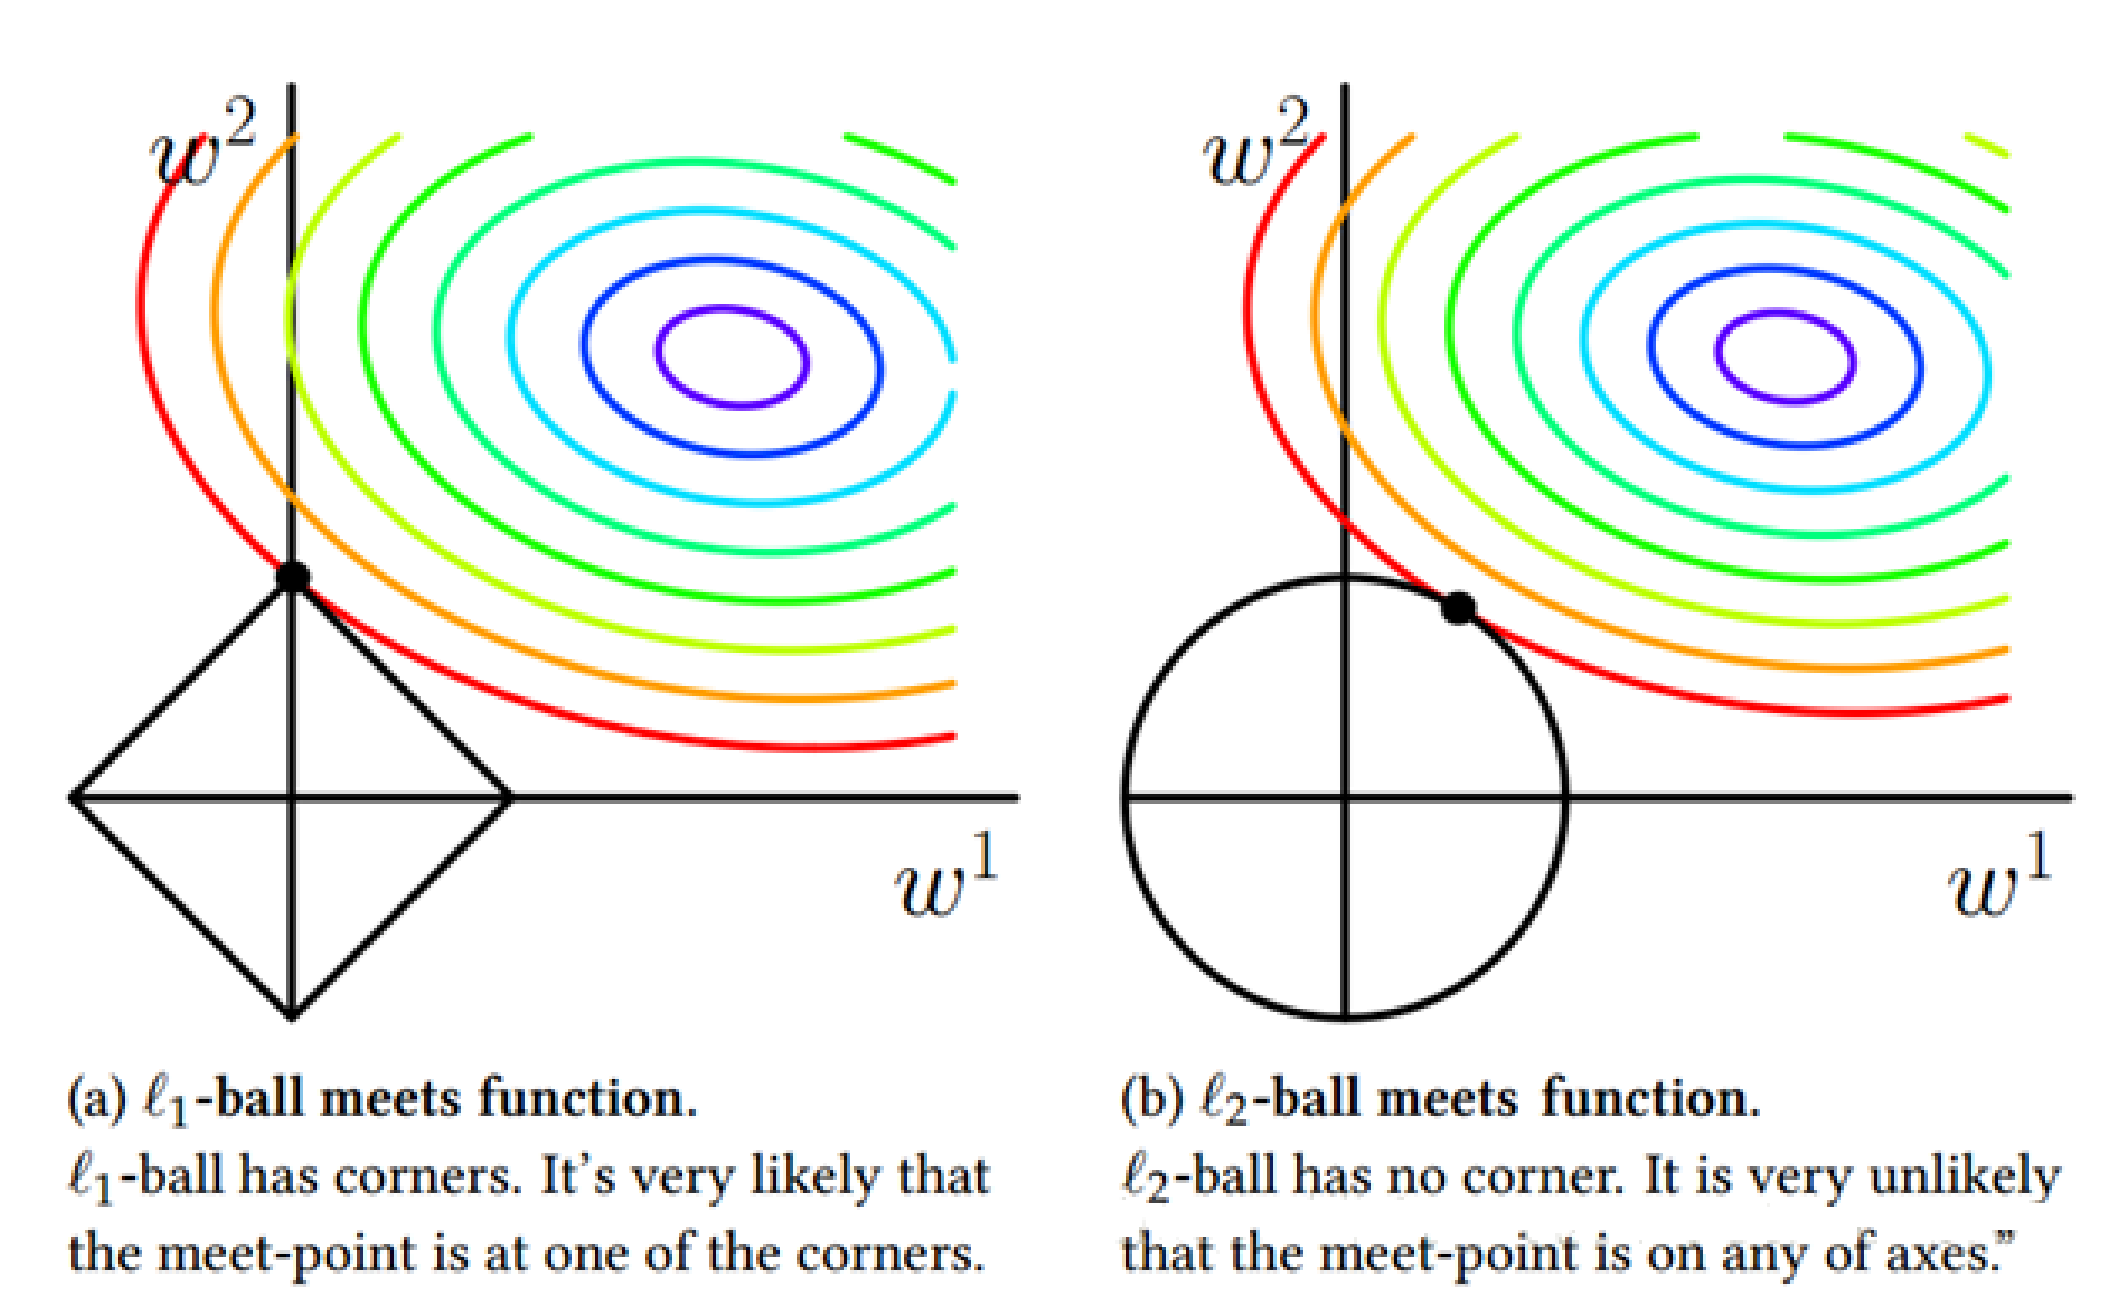
\includegraphics[width=0.7\linewidth]{l1_l2_sparsity}
\caption{Comparison of a L1 and L2 penalties.}
\label{fig:l1_l2_sparsity}
\end{figure}

\subsection{Drop-out}
Drop-out \cite{Hinton_Dropout_2012} is used to regularize large fully-connected layers within neural networks. When training with drop-out, a randomly selected subset of activations are set to zero within each layer. 
Drop-out will improves the inference ability of neural networks while keeps the complexity unchanged. 
Extensive experiments show that drop-out improves the network's generalization ability.
Fig.~\ref{fig:bp_dropout} illustrates the drop-out instance.

\begin{figure}
\centering
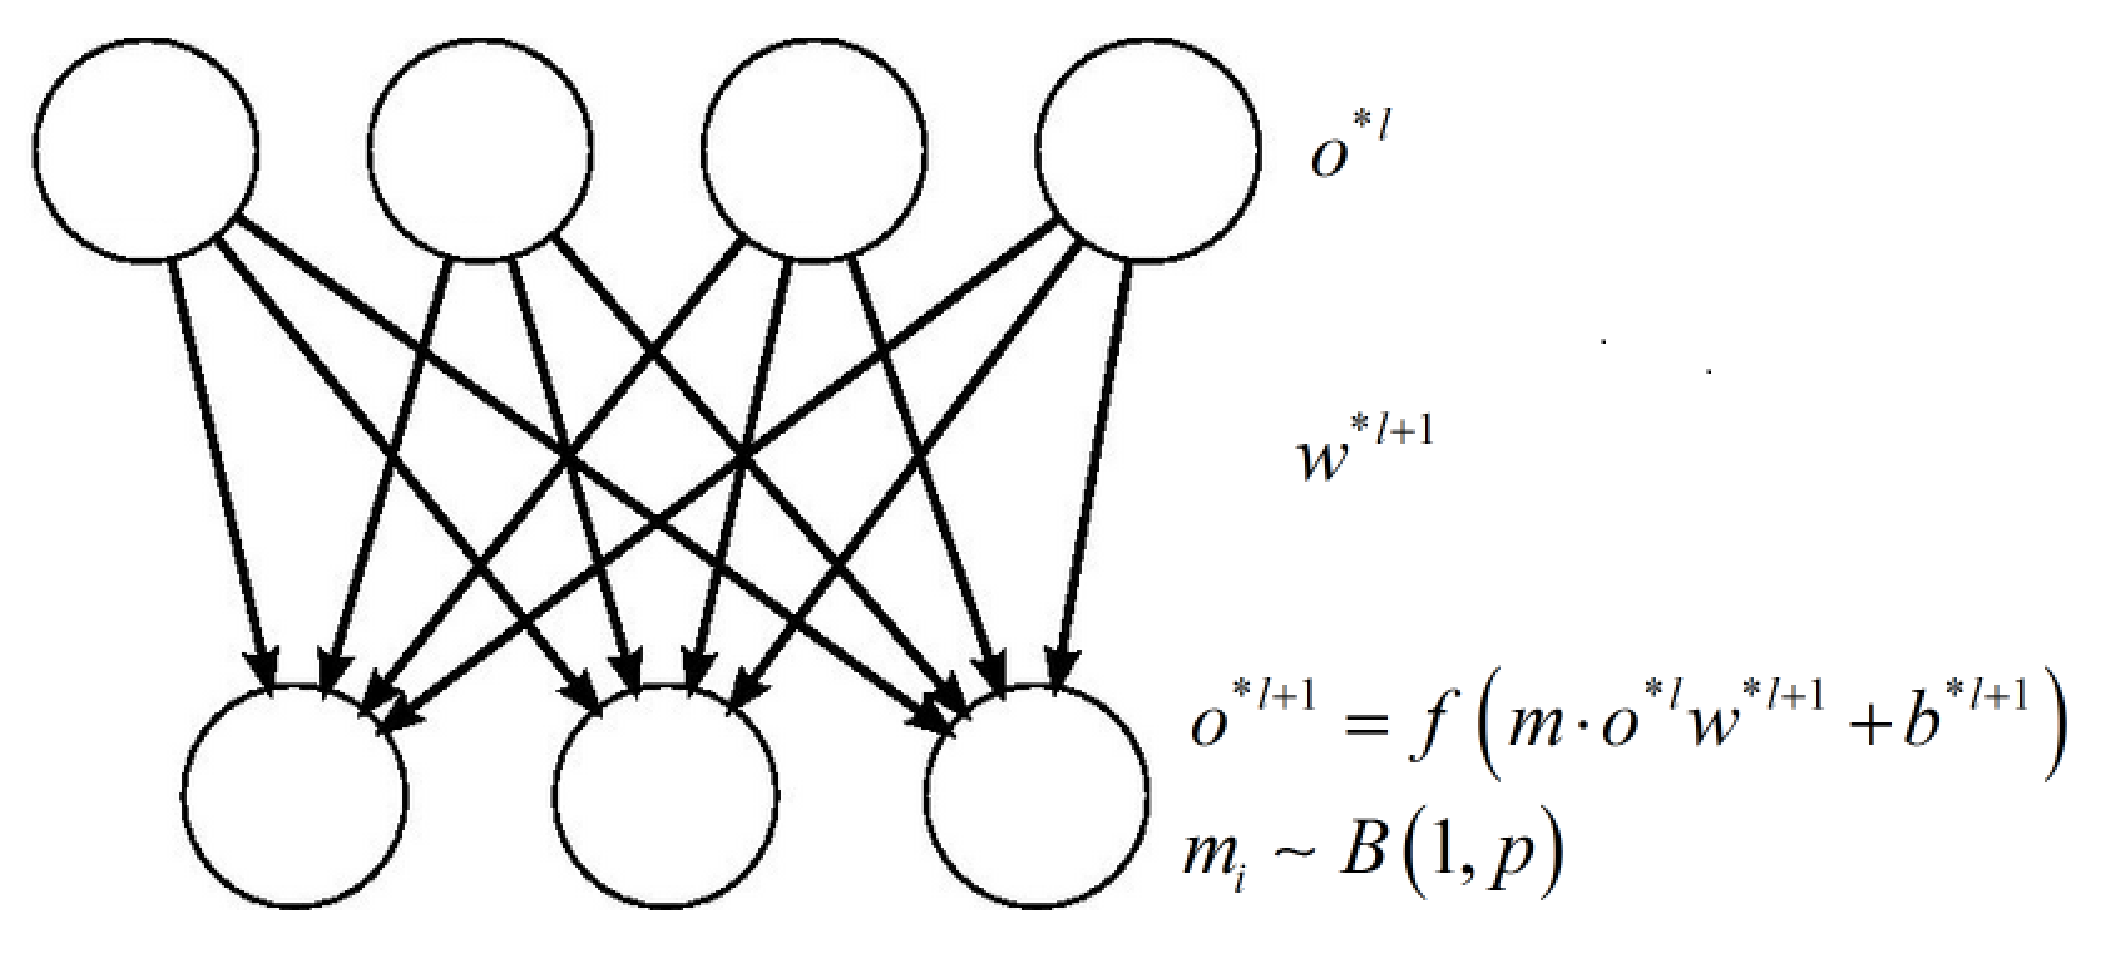
\includegraphics[width=0.8\linewidth]{dropout}
\caption{Illustration of drop-out training strategy for neural network.}
\label{fig:bp_dropout}
\end{figure}

Consider the drop-out layer $l + 1$ (as Fig.~\ref{fig:bp_dropout} indicated), in training stage, we generate the random mask vector $m$ for $o^{*l}$ satisfied Bernoulli distribution $B\left( {1,p} \right)$. The activate output $o^{l + 1}$ need combine the mask vector as Fig.~\ref{fig:bp_dropout} shown. The $\delta ^{*l}$ should be calculated by Eq.~\ref{equ:bp_dropout_delta}.  

\begin{equation}
\label{equ:bp_dropout_delta}
\begin{aligned}
{\delta ^{*l}}_j &= \frac{{\partial JS}}{{\partial {s^{*l}}_j}}\\
 &= \sum\limits_k {\frac{{\partial JS}}{{\partial {s^{*l + 1}}_k}}\frac{{\partial {s^{*l + 1}}_k}}{{\partial {o^{*l}}_j}}\frac{{\partial {o^{*l}}_j}}{{\partial {s^{*l}}_j}}} \\
 &= \sum\limits_k {\frac{{\partial JS}}{{\partial {s^{*l + 1}}_k}}\frac{{\partial \left( {m \cdot {o^{*l}}{w^{*l + 1}}_{\_k}} \right)}}{{\partial {o^{*l}}_j}}\frac{{\partial {o^{*l}}_j}}{{\partial {s^{*l}}_j}}} \\
 &= {m_j}\sum\limits_k {\frac{{\partial JS}}{{\partial {s^{*l + 1}}_k}}\frac{{\partial \left( {{o^{*l}}{w^{*l + 1}}_{\_k}} \right)}}{{\partial {o^{*l}}_j}}\frac{{\partial {o^{*l}}_j}}{{\partial {s^{*l}}_j}}} \\
 &= {m_j}\sum\limits_k {{\delta ^{*l + 1}}_k{w^{*l + 1}}_{jk}{f^{'}}\left( {{s^{*l}}_j} \right)} \\
 \Rightarrow {\delta ^{*l}} &= {f^{'}}\left( {{s^{*l}}} \right) \cdot m \cdot \left( {{\delta ^{*l + 1}}{{\left( {{w^{*l + 1}}} \right)}^t}} \right)
\end{aligned}
\end{equation}

The gradient of $w^{*l + 1}$ can be computed by 

\begin{equation}
\label{equ:bp_dropout_gradient}
\frac{{\partial J}}{{\partial {w^{*j + 1}}}} = \left( {m \cdot {o^{*l}}} \right){\delta ^{*l + 1}}
\end{equation}

During in inference stage, the activate output $o^{*l + 1}$ can be formalized by Eq.~\ref{equ:bp_dropout_expectation}.

\begin{equation}
\label{equ:bp_dropout_expectation}
\begin{aligned}
{o^{*l + 1}} &= E\left( {f\left( {{s^{*l + 1}}} \right)} \right)\\
 &= E\left( {f\left( {m{o^{*l}}{w^{*l + 1}} + {b^{*l + 1}}} \right)} \right)
\end{aligned}
\end{equation}

We have two strategies to compute the expectation: mean approximation and sampling approximation. 
For mean approximation, we have Eq.~\ref{equ:bp_dropout_mean_approximation}.

\begin{equation}
\label{equ:bp_dropout_mean_approximation}
\begin{aligned}
{o^{*l + 1}} &= E\left( {f\left( {{s^{*l + 1}}} \right)} \right)\\
 &= E\left( {f\left( {m{o^{*l}}{w^{*l + 1}} + {b^{*l + 1}}} \right)} \right)\\
 &\approx f\left( {E\left( {m \cdot {o^{*l}}{w^{*l + 1}} + {b^{*l + 1}}} \right)} \right)\\
 &= f\left( {E\left( {m \cdot {o^{*l}}{w^{*l + 1}} + {b^{*l + 1}}} \right)} \right)\\
 &= f\left( {p{o^{*l}}{w^{*l + 1}} + {b^{*l + 1}}} \right)
\end{aligned}
\end{equation}

For sampling approximation, we have Eq.~\ref{equ:bp_dropout_sampling_approximation}.

\begin{equation}
\label{equ:bp_dropout_sampling_approximation}
\begin{aligned}
let\ u &= m{o^{*l}}{w^{*l + 1}}\\
{u_i} &= m{o^{*l}}{w^{*l + 1}}_{\_i}\\
 &= \sum\limits_k {{m_k}{o^{*l}}_k{w^{*l + 1}}_{ki}} \\
 \Rightarrow &{u_i} \sim N\left( {p\sum\limits_k {{o^{*l}}_k{w^{*l + 1}}_{ki}} ,p\left( {1 - p} \right)\sum\limits_k {{{\left( {{o^{*l}}_k{w^{*l + 1}}_{ki}} \right)}^2}} } \right)\\
 \Rightarrow &{u_i} \sim N\left( {p{{\left( {{o^{*l}}{w^{*l + 1}}} \right)}_i},p\left( {1 - p} \right)\left( {{o^{*l}} \cdot {o^{*l}}} \right){{\left( {{w^{*l + 1}} \cdot {w^{*l + 1}}} \right)}_{\_i}}} \right)\\
 \Rightarrow &u \sim N\left( {p{o^{*l}}{w^{*l + 1}},p\left( {1 - p} \right)\left( {{o^{*l}} \cdot {o^{*l}}} \right)\left( {{w^{*l + 1}} \cdot {w^{*l + 1}}} \right)} \right)
\end{aligned}
\end{equation}
notice that the variance in the norm distribution is not covariance, it is just a vector consisted of variances of all dimensions. We sample $n$ of $u$ from the norm distribution and compute the average value for $o^{*l + 1}$ as Eq.~\ref{equ:bp_dropout_sampling_o}.

\begin{equation}
\label{equ:bp_dropout_sampling_o}
\begin{aligned}
{o^{*l + 1}} &= E\left( {f\left( {m{o^{*l}}{w^{*l + 1}} + {b^{*l + 1}}} \right)} \right)\\
 &= \frac{1}{n}\sum\limits_{j = 0}^{n - 1} {f\left( {{u^{*j}} + {b^{*l + 1}}} \right)} 
\end{aligned}
\end{equation}

\subsection{Drop-connect}
Drop-connect\cite{LiWan_Dropconnect_2013} is the generalization of drop-out in which each connection, rather than each output unit, can be dropped with probability $1 - p$. Drop-connect is similar to drop-out as it introduces dynamic sparsity within the model, but differs in that the sparsity is on the weights $w$, rather than the output vectors of a layer. In other words, the fully connected layer with drop-connect becomes a sparsely connected layer in which the connections are chosen at random during the training stage. Note that this is not equivalent to setting $w$ to be a fixed sparse matrix during training. 
Fig.~\ref{fig:bp_dropconnect} illustrates the drop-connect instance.

\begin{figure}
\centering
\includegraphics[width=0.85\linewidth]{dropconnect}
\caption{Illustration of drop-connect training strategy for neural network.}
\label{fig:bp_dropconnect}
\end{figure}

For a drop-connect layer $l + 1$, the output is given as:

\begin{equation}
\label{equ:bp_dropconnect_layer_output}
{o^{*l + 1}} = f\left( {{o^{*l}}\left( {m \cdot {w^{*l + 1}}} \right) + {b^{*l + 1}}} \right)
\end{equation}
where $m$ is a binary matrix encoding the connection information and ${m_{ij}} \sim B\left( {1,p} \right)$. Each element of the mask $m$ is drawn independently for each example or batch samples during training. Additionally, the biases can be masked out or not during training. Here we only discuss the weight masked strategy.

Similar to drop-out, we calculate the ${\delta ^{*l}}_j$ by Eq.~\ref{equ:bp_dropconnect_delta}. Note that the gradient of weight $\Delta w^{*l + 1}$ need to multiply by mask matrix $m$.

\begin{equation}
\label{equ:bp_dropconnect_delta}
\begin{aligned}
{\delta ^{*l}}_j &= \frac{{\partial JS}}{{\partial {s^{*l}}_j}}\\
 &= \sum\limits_k {\frac{{\partial JS}}{{\partial {s^{*l + 1}}_k}}\frac{{\partial {s^{*l + 1}}_k}}{{\partial {o^{*l}}_j}}\frac{{\partial {o^{*l}}_j}}{{\partial {s^{*l}}_j}}} \\
 &= \sum\limits_k {\frac{{\partial JS}}{{\partial {s^{*l + 1}}_k}}\frac{{\partial \left( {{o^{*l}}\left( {{m_{\_k}} \cdot {w^{*l + 1}}_{\_k}} \right)} \right)}}{{\partial {o^{*l}}_j}}\frac{{\partial {o^{*l}}_j}}{{\partial {s^{*l}}_j}}} \\
 &= \sum\limits_k {{\delta ^{*l + 1}}_k{m_{jk}}{w^{*l + 1}}_{jk}{f^{'}}\left( {{s^{*l}}_j} \right)} \\
\Rightarrow {\delta ^{*l}} &= {f^{'}}\left( {{s^{*l}}} \right) \cdot \left( {{\delta ^{*l + 1}}{{\left( {m \cdot {w^{*l + 1}}} \right)}^t}} \right)
\end{aligned}
\end{equation}

The gradient of $w^{*l + 1}$ can be computed by 

\begin{equation}
\label{equ:bp_dropconnect_gradient}
\frac{{\partial J}}{{\partial {w^{*j + 1}}}} = m \cdot \left( {{{\left( {{o^{*l}}} \right)}^t}{\delta ^{*l + 1}}} \right)
\end{equation}

The inference of drop-connect is very similar to drop-out. Here we only list the formulas: Eq.~\ref{equ:bp_dropconnect_mean_approximation} for mean approximation while Eq.~\ref{equ:bp_dropconnect_sampling_approximation} for sampling approximation.

\begin{equation}
\label{equ:bp_dropconnect_mean_approximation}
\begin{aligned}
{o^{*l + 1}} &= E\left( {f\left( {{s^{*l + 1}}} \right)} \right)\\
 &= E\left( {f\left( {{o^{*l}}\left( {m \cdot {w^{*l + 1}}} \right) + {b^{*l + 1}}} \right)} \right)\\
 &\approx f\left( {E\left( {{o^{*l}}\left( {m \cdot {w^{*l + 1}}} \right) + {b^{*l + 1}}} \right)} \right)\\
 &= f\left( {E\left( {{o^{*l}}\left( {m \cdot {w^{*l + 1}}} \right) + {b^{*l + 1}}} \right)} \right)\\
 &= f\left( {p{o^{*l}}{w^{*l + 1}} + {b^{*l + 1}}} \right)
\end{aligned}
\end{equation}

\begin{equation}
\label{equ:bp_dropconnect_sampling_approximation}
\begin{aligned}
{o^{*l + 1}} &= f\left( {{o^{*l}}\left( {m \cdot {w^{*l + 1}}} \right) + {b^{*l + 1}}} \right)\\
let u &= {o^{*l}}\left( {m \cdot {w^{*l + 1}}} \right)\\
{u_i} &= {o^{*l}}\left( {{m_{\_i}} \cdot {w^{*l + 1}}_{\_i}} \right)\\
 &= \sum\limits_k {{o^{*l}}_k{m_{ki}}{w^{*l + 1}}_{ki}} \\
 \Rightarrow& {u_i} \sim N\left( {p\sum\limits_k {{o^{*l}}_k{w^{*l + 1}}_{ki}} ,p\left( {1 - p} \right)\sum\limits_k {{{\left( {{o^{*l}}_k{w^{*l + 1}}_{ki}} \right)}^2}} } \right)\\
 \Rightarrow& {u_i} \sim N\left( {p{{\left( {{o^{*l}}{w^{*l + 1}}} \right)}_i},p\left( {1 - p} \right)\left( {{o^{*l}} \cdot {o^{*l}}} \right){{\left( {{w^{*l + 1}} \cdot {w^{*l + 1}}} \right)}_{\_i}}} \right)\\
 \Rightarrow& u \sim N\left( {p{o^{*l}}{w^{*l + 1}},p\left( {1 - p} \right)\left( {{o^{*l}} \cdot {o^{*l}}} \right)\left( {{w^{*l + 1}} \cdot {w^{*l + 1}}} \right)} \right)
\end{aligned}
\end{equation}

In fact, drop-out is a special case of drop-connect. We can prove by Eq.~

\begin{equation}
\label{equ:drop_out_connect_relation}
\begin{aligned}
let \quad {{\tilde m}_{i\_}} &= {m_i}\\
{\delta ^{*l}} &= {f^{'}}\left( {{s^{*l}}} \right) \cdot m \cdot \left( {{\delta ^{*l + 1}}{{\left( {{w^{*l + 1}}} \right)}^t}} \right)\\
 &= {f^{'}}\left( {{s^{*l}}} \right) \cdot {\left( {{{\tilde m}_{\_0}}} \right)^t} \cdot \left( {{\delta ^{*l + 1}}{{\left( {{w^{*l + 1}}} \right)}^t}} \right)\\
 &= {f^{'}}\left( {{s^{*l}}} \right) \cdot \left( {{\delta ^{*l + 1}}\left( {\left[ {\begin{array}{*{20}{c}}
{{{\left( {{{\tilde m}_{\_0}}} \right)}^t}}\\
{...}\\
{{{\left( {{{\tilde m}_{\_0}}} \right)}^t}}
\end{array}} \right]{{\left( {{w^{*l + 1}}} \right)}^t}} \right)} \right)\\
 &= {f^{'}}\left( {{s^{*l}}} \right) \cdot \left( {{\delta ^{*l + 1}}\left( {{{\tilde m}^t}{{\left( {{w^{*l + 1}}} \right)}^t}} \right)} \right)\\
 &= {f^{'}}\left( {{s^{*l}}} \right) \cdot \left( {{\delta ^{*l + 1}}\left( {{{\left( {\tilde m{w^{*l + 1}}} \right)}^t}} \right)} \right)\\
\frac{{\partial J}}{{\partial {w^{*j + 1}}}} &= {\left( {m \cdot {o^{*l}}} \right)^t}{\delta ^{*l + 1}}\\
 &= \left( {{m^t} \cdot {{\left( {{o^{*l}}} \right)}^t}} \right){\delta ^{*l + 1}}\\
 &= \left( {\left( {{{\tilde m}_{\_0}}} \right) \cdot {{\left( {{o^{*l}}} \right)}^t}} \right)\\
 &= \left[ {{{\tilde m}_{\_0}},...,{{\tilde m}_{\_0}}} \right]\left( {{{\left( {{o^{*l}}} \right)}^t}{\delta ^{*l + 1}}} \right)\\
 &= \tilde m \cdot \left( {{{\left( {{o^{*l}}} \right)}^t}{\delta ^{*l + 1}}} \right)
\end{aligned}
\end{equation}

\subsection{Batch Normalizing}
We define \emph{Internal Covariate Shift} as the change in the distribution of network activations due to the change in network parameters during training \footnote{This section refers to the paper of \cite{Sergey_BatchNorm_2015}.}.
To improve the training, we seek to reduce
 

\begin{equation}
\begin{aligned}
{\left( {{{\hat s}^{*l + 1}}} \right)^{*i}} &= \frac{{{o^{*l}} - E\left( {\left( {{o^{*l}}} \right)} \right)}}{{\sqrt {{\mathop{\rm var}} \left( {{o^{*l}}} \right) + \varepsilon } }}\\
{\left( {{s^{*l + 1}}} \right)^{*i}} &= {\gamma ^{*l + 1}}{\left( {{{\hat s}^{*l + 1}}} \right)^{*i}} + \beta 
\end{aligned}
\end{equation}

\begin{equation}
\begin{aligned}
\frac{{\partial J}}{{\partial {{\left( {{o^{*l}}} \right)}^{*i}}}} &= \frac{{\partial J}}{{\partial {{\left( {{{\hat s}^{*l + 1}}} \right)}^{*i}}}}\frac{{\partial {{\left( {{{\hat s}^{*l + 1}}} \right)}^{*i}}}}{{\partial {{\left( {{o^{*l}}} \right)}^{*i}}}} + \frac{{\partial J}}{{\partial E\left( {{o^{*l}}} \right)}}\frac{{\partial E\left( {{o^{*l}}} \right)}}{{\partial {{\left( {{o^{*l}}} \right)}^{*i}}}} + \frac{{\partial J}}{{\partial D\left( {{o^{*l}}} \right)}}\frac{{\partial D\left( {{o^{*l}}} \right)}}{{\partial {{\left( {{o^{*l}}} \right)}^{*i}}}}\\
\frac{{\partial J}}{{\partial {{\left( {{{\hat s}^{*l + 1}}} \right)}^{*\hat i}}}} &= \frac{{\partial J}}{{\partial {{\left( {{s^{*l + 1}}} \right)}^{*i}}}} \cdot \frac{{\partial {{\left( {{s^{*l + 1}}} \right)}^{*i}}}}{{\partial {{\left( {{{\hat s}^{*l + 1}}} \right)}^{*i}}}}\\
\frac{{\partial J}}{{\partial E\left( {{o^{*l}}} \right)}} &= \sum\limits_{\hat i = 0}^{m - 1} {\frac{{\partial J}}{{\partial {{\left( {{{\hat s}^{*l + 1}}} \right)}^{*\hat i}}}} \cdot \frac{{\partial {{\left( {{{\hat s}^{*l + 1}}} \right)}^{*\hat i}}}}{{\partial E\left( {{o^{*l}}} \right)}}}  + \frac{{\partial J}}{{\partial D\left( {{o^{*l}}} \right)}} \cdot \frac{{\partial D\left( {{o^{*l}}} \right)}}{{\partial E\left( {{o^{*l}}} \right)}}\\
\frac{{\partial E\left( {{o^{*l}}} \right)}}{{\partial {{\left( {{o^{*l}}} \right)}^{*i}}}} &= \frac{1}{m}\\
\frac{{\partial J}}{{\partial D\left( {{o^{*l}}} \right)}} &= \sum\limits_{\hat i = 0}^{m - 1} {\frac{{\partial J}}{{\partial {{\left( {{{\hat s}^{*l + 1}}} \right)}^{*\hat i}}}} \cdot \frac{{\partial {{\left( {{{\hat s}^{*l + 1}}} \right)}^{*\hat i}}}}{{\partial D\left( {{o^{*l}}} \right)}}} \\
\frac{{\partial D\left( {{o^{*l}}} \right)}}{{\partial {{\left( {{o^{*l}}} \right)}^{*i}}}} &= \frac{2}{m}\left( {{{\left( {{o^{*l}}} \right)}^{*i}} - E\left( {{o^{*l}}} \right)} \right)\\
\frac{{\partial D\left( {{o^{*l}}} \right)}}{{\partial E\left( {{o^{*l}}} \right)}} &= \frac{{ - 2}}{m}\sum\limits_{i = 0}^{m - 1} {\left( {{{\left( {{o^{*l}}} \right)}^{*\hat i}} - E\left( {{o^{*l}}} \right)} \right)}  =  - \sum\limits_{i = 0}^{m - 1} {\frac{{\partial D\left( {{o^{*l}}} \right)}}{{\partial {{\left( {{o^{*l}}} \right)}^{*i}}}}} 
\end{aligned}
\end{equation}

\begin{equation}
\begin{aligned}
\frac{{\partial J}}{{\partial {{\left( {{{\hat s}^{*l + 1}}} \right)}^{*\hat i}}}} &= {\left( {{\delta ^{*l + 1}}} \right)^{*i}}{\gamma ^{*l + 1}}\\
\frac{{\partial {{\left( {{{\hat s}^{*l + 1}}} \right)}^{*i}}}}{{\partial {{\left( {{o^{*l}}} \right)}^{*i}}}} &= \frac{1}{{\sqrt {D\left( {{o^{*l}}} \right) + \varepsilon } }}\\
\frac{{\partial {{\left( {{{\hat s}^{*l + 1}}} \right)}^{*\hat i}}}}{{\partial E\left( {{o^{*l}}} \right)}} &= \frac{{ - 1}}{{\sqrt {D\left( {{o^{*l}}} \right) + \varepsilon } }}\\
\frac{{\partial {{\left( {{{\hat s}^{*l + 1}}} \right)}^{*i}}}}{{\partial D\left( {{o^{*l}}} \right)}} &= \left( {{{\left( {{o^{*l}}} \right)}^{*i}} - E\left( {{o^{*l}}} \right)} \right) \cdot \frac{{ - 1}}{2}{\left( {D\left( {{o^{*l}}} \right) + \varepsilon } \right)^{\frac{{ - 3}}{2}}}\\
\frac{{\partial J}}{{\partial {\gamma ^{*l}}}} &= \sum\limits_{\hat i = 0}^{m - 1} {\frac{{\partial J}}{{\partial {{\left( {{{\hat s}^{*l}}} \right)}^{*\hat i}}}} \cdot \frac{{\partial {{\left( {{{\hat s}^{*l}}} \right)}^{*\hat i}}}}{{\partial {\gamma ^{*l}}}}} = \sum\limits_{\hat i = 0}^{m - 1} {{{\left( {{\delta ^{*l}}} \right)}^{*\hat i}} \cdot {{\left( {{{\hat s}^{*l}}} \right)}^{*\hat i}}} \\
\frac{{\partial J}}{{\partial \beta }} &= \sum\limits_{\hat i = 0}^{m - 1} {\frac{{\partial J}}{{\partial {{\left( {{{\hat s}^{*l}}} \right)}^{*\hat i}}}}}  = \sum\limits_{\hat i = 0}^{m - 1} {{{\left( {{\delta ^{*l}}} \right)}^{*\hat i}}} 
\end{aligned}
\end{equation}

\section{Recurrent Neural Network}
\label{sec:rnn}
In the previous section we considered feed-forward neural networks whose connection s did not form cycles. If we relax this condition, and allow cyclical connections as well, we obtain recurrent neural networks (RNNs).
As with feed-forward networks, many varieties of RNN have been proposed, such as Elman networks, Jordan networks, time delay neural networks and echo state networks.
In this section, we focus on a simple RNN containing a single, self connected hidden layer, as shown in Fig.~\ref{fig:rnn_example}.

\begin{figure}
\centering
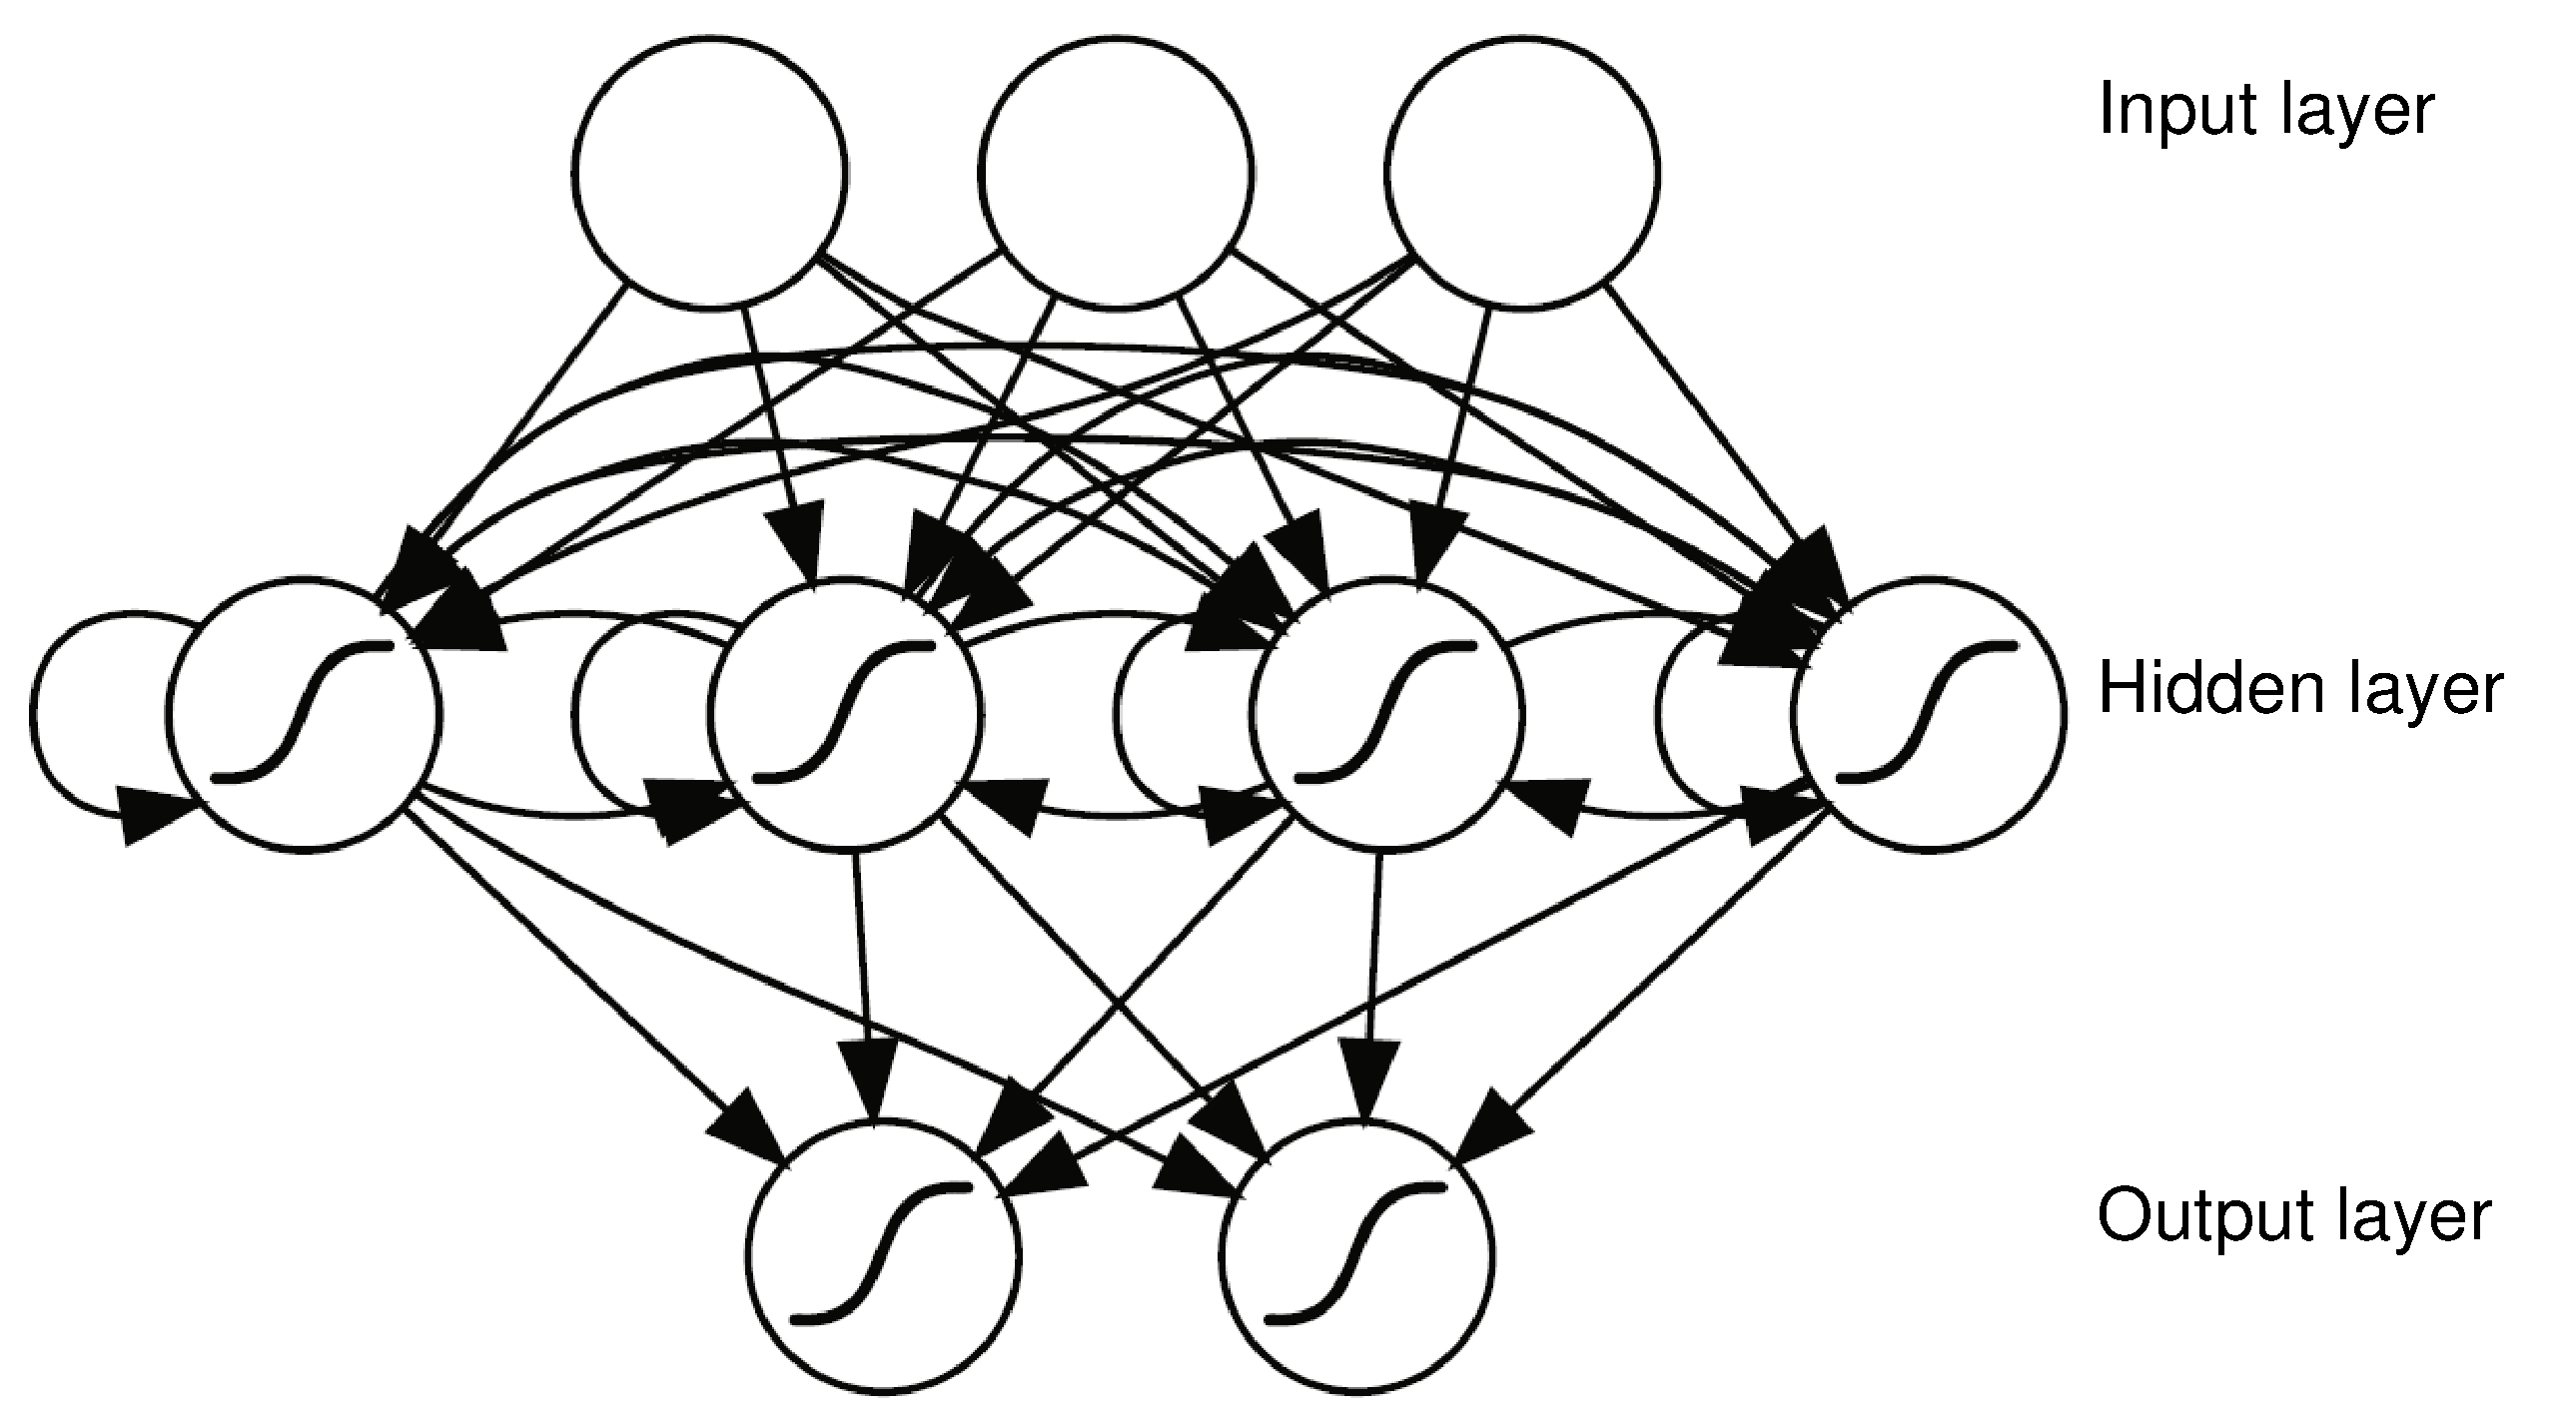
\includegraphics[width=0.7\linewidth]{rnn}
\caption{Illustration of a recurrent neural network. Note that the connections of one hidden unit are full to other hidden units. The figure omits some connections for better vision.}
\label{fig:rnn_example}
\end{figure}

While the difference between a multilayer perceptron and an RNN may seem trivial, the implications for sequence learning are far-reaching.
An MLP can only map from input to output vectors, whereas an RNN can in principle map from the entire \emph{history} of previous inputs to each output.
Indeed, the equivalent result to the universal approximation theory for MLPs is that an RNN with a sufficient number of hidden units can approximate any measurable sequence-to-sequence mapping to arbitrary accuracy \cite{Hammer_RNN_Capability_2000}.
The key point is that the recurrent connections allow a 'memory' of previous inputs to persist in the network's internal state, and thereby influence the network output.

A useful way to visualise RNNs is to to consider the update graph formed by 'unfolding' the network along the input sequence. Fig.~\ref{fig:unfolded_rnn_example} shows part of an unfolded RNN.
Viewing RNNs as unfolded graphs makes it easier to generalise to networks with more complex update dependencies.

\begin{figure}
\centering
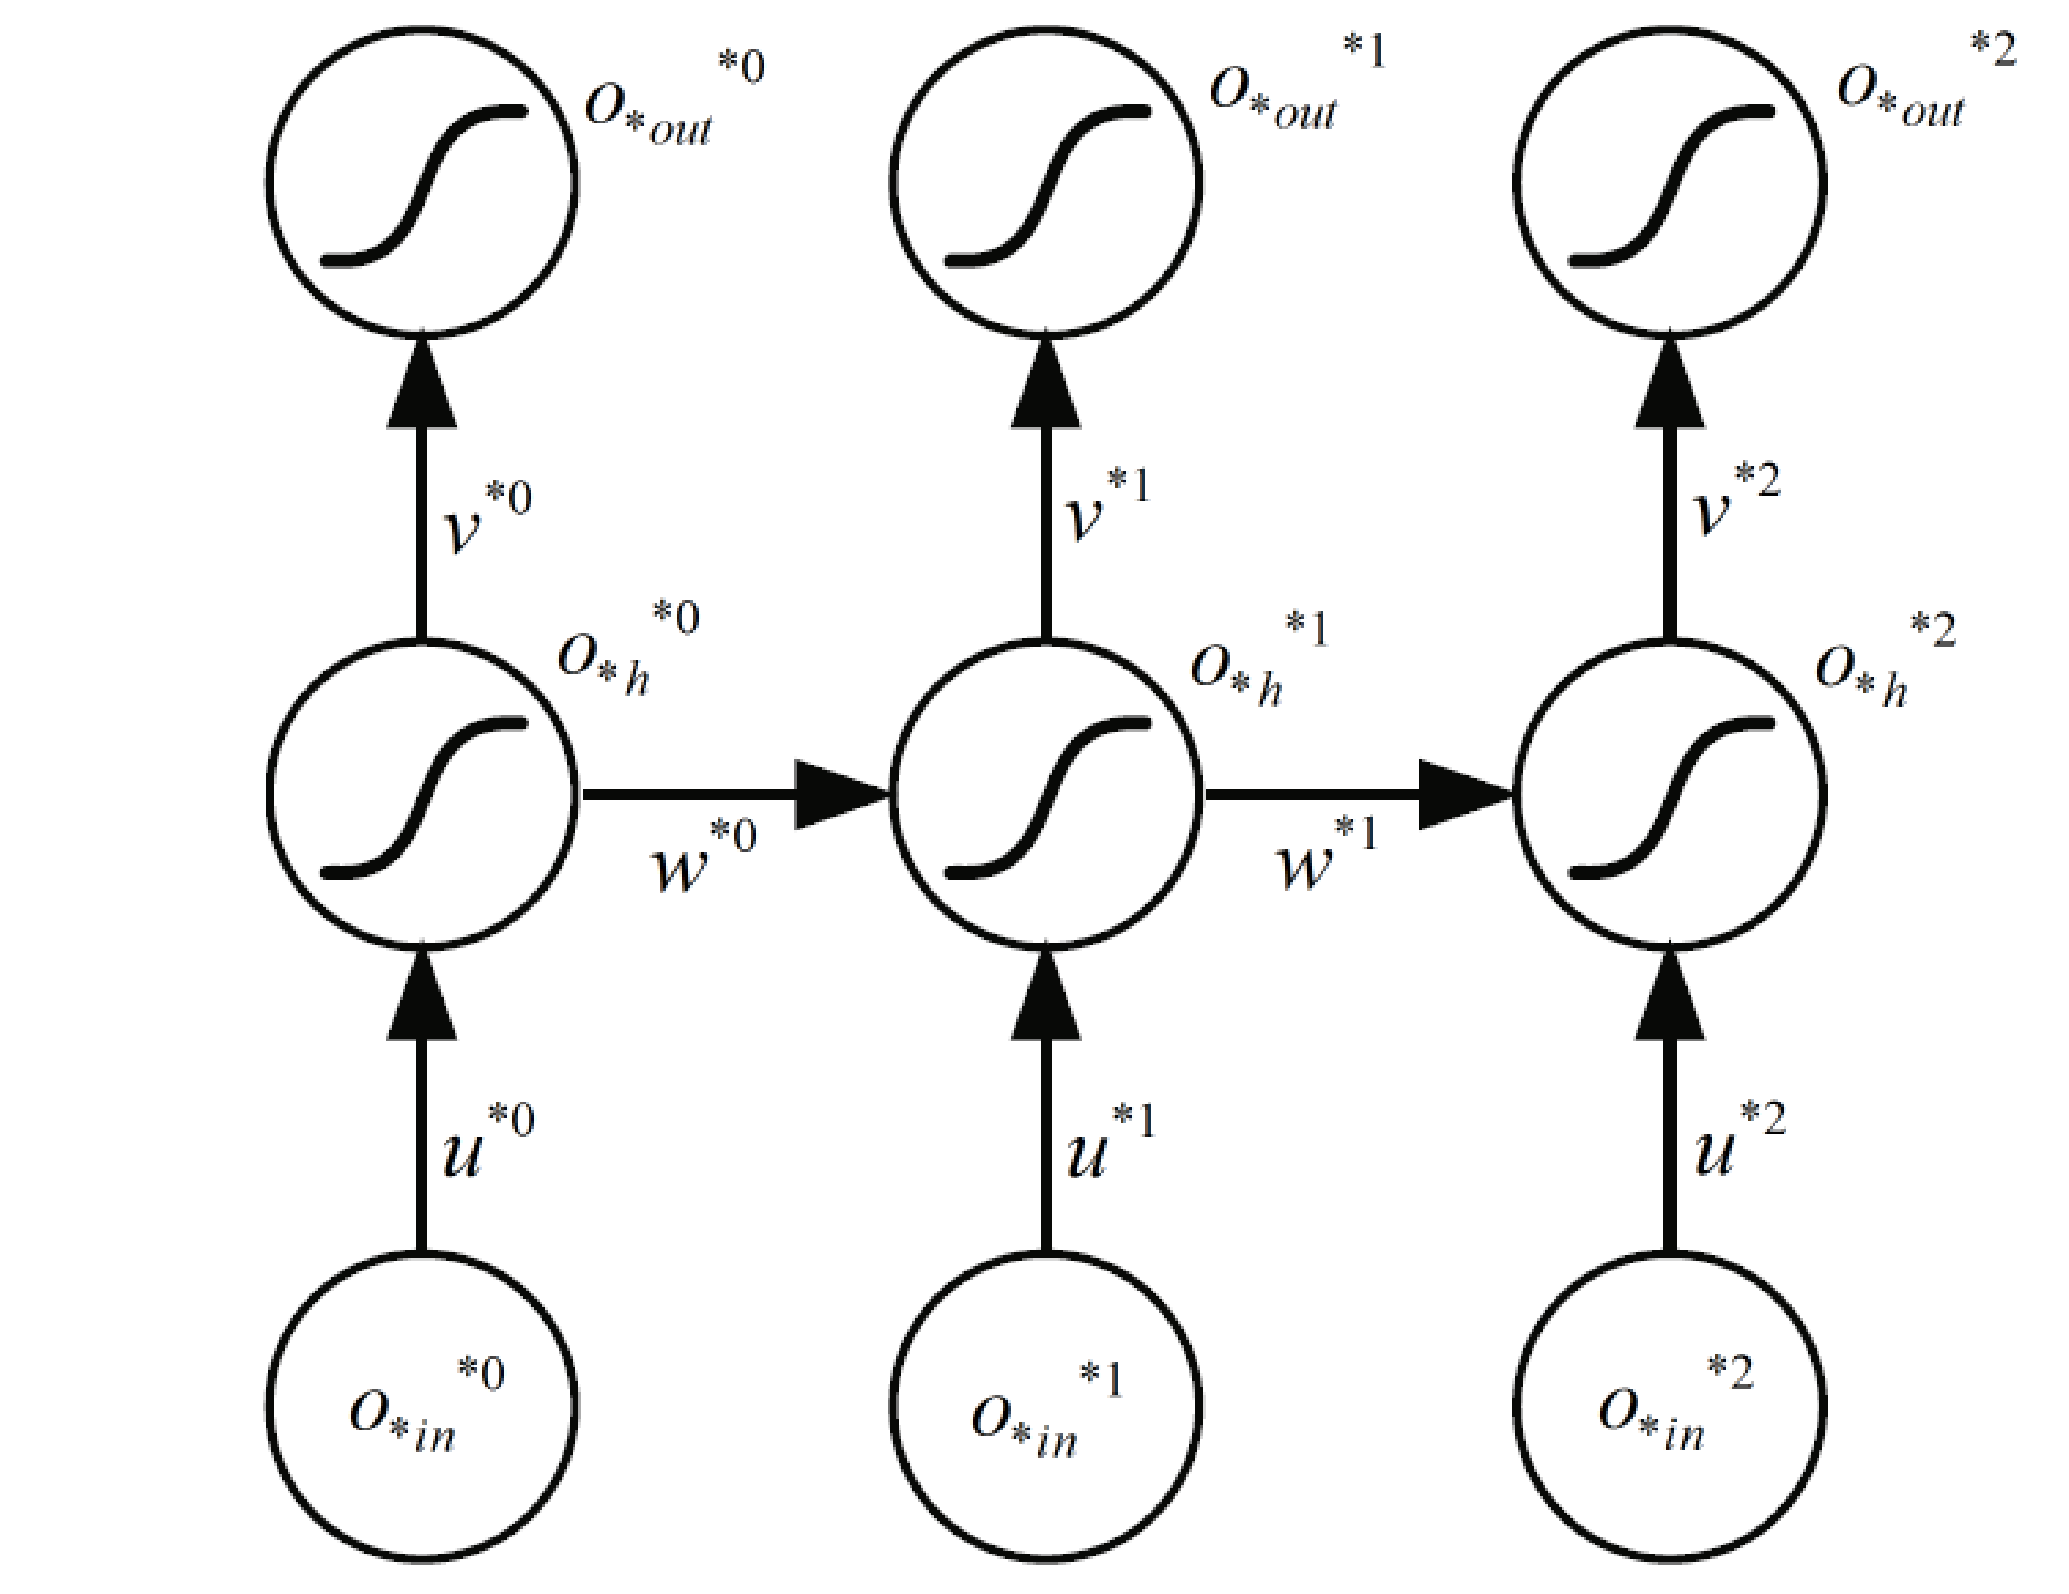
\includegraphics[width=0.6\linewidth]{unfolded_rnn}
\caption{An unfolded RNN.}
\label{fig:unfolded_rnn_example}
\end{figure}

\subsection{Forward Pass}
The forward pass of an RNN is the same as that of a multilayer perceptron with a single hidden layer, except that activations arrive at the hidden layer from both the current external input and the hidden layer activations from the previous time step.
Consider a length $T$ input sequence $o_{*in}$ presented to an RNN with $I$ input units, $J$ hidden units, and $K$ output units. Let ${\left( {{o_{*in}}} \right)_i}^{*t}$ be the value of input $i$ at time $t$, and let ${\left( {{s}} \right)_j}^{*t}$ and ${\left( {{o}} \right)_j}^{*t}$ be respectively the network input to unit $j$ at time $t$ and the activation of unit $j$ at time $t$. For the hidden units we have

\begin{equation}
\label{equ:rnn_hidden_output}
\begin{aligned}
{\left( {{s_{*h}}} \right)_j}^{*t} &= \sum\limits_{\hat i} {{u_{\hat ij}}{{\left( {{o_{*in}}} \right)}_{\hat i}}^{*t}}  + \sum\limits_{\hat l} {{w_{\hat lj}}{{\left( {{o_{*h}}} \right)}_{\hat l}}^{*t - 1}}  + {b_j}\\
{\left( {{o_{*h}}} \right)_j}^{*t} &= f\left( {{{\left( {{s_{*h}}} \right)}_j}^{*t}} \right)
\end{aligned}
\end{equation}
where $\hat l$ denotes the index of previous time, $u, w, v$ denote the weight of input-hidden, weight of hidden-hidden and weight of hidden-output. $b_{*h}$ denotes the bias for hidden layer.

The complete sequence of hidden activations can be calculated by starting at $t = 0$ and recursively applying Eq.~\ref{equ:rnn_hidden_output}, incrementing $t$ at each step.
Note that this requires initial value ${{{\left( {{o_{*h}}} \right)}_j}^{*-1}}$ to be chosen for the hidden units, corresponding to the networks's state before it receives any information from the data sequence.
In this book, the initial values are always set to zero.

The network inputs to the output units can be calculated at the same time as the hidden activations:

\begin{equation}
\label{equ:rnn_output_layer_output}
\begin{aligned}
{\left( {{s_{*out}}} \right)_k}^{*t} &= \sum\limits_{\hat j} {{v_{\hat jk}}{{\left( {{o_{*h}}} \right)}_{\hat j}}^{*t}}  + {c_k}\\
{\left( {{o_{*out}}} \right)_k}^{*t} &= f\left( {{{\left( {{s_{*out}}} \right)}_k}^{*t}} \right)
\end{aligned}
\end{equation}

\subsection{Backward Pass}
Given the partial derivatives of some differentiable loss function $loss$ with respect to the network outputs, the next step is to determine the derivatives with respect to the weights. Two well-know algorithms have been devised to efficiently calculate weight derivatives for RNNs: real time recurrent learning and back-propagation through time (BPTT).
We focus on BPTT since it is both conceptually simpler and more efficient in computation time (though not in memory).

The cost function of the RNN model on one sequence is 

\begin{equation}
\label{equ:rnn_cost_function}
JS = \sum\limits_{t = 0}^{T - 1} {loss\left( {{y^{*t}},{{\left( {{o_{*out}}} \right)}^{*t}}} \right)} 
\end{equation}

The partial derivative for $JS$ about ${{u_{ij}}}$ is 

\begin{equation}
\label{equ:rnn_derivative_u}
\begin{aligned}
\frac{{\partial JS}}{{\partial {u_{ij}}}} &= \frac{{\partial \sum\limits_{t = 0}^{T - 1} {loss\left( {{y^{*t}},{{\left( {{o_{*out}}} \right)}^{*t}}} \right)} }}{{\partial {u_{ij}}}}\\
 &= \sum\limits_{t = 0}^{T - 1} {\frac{{\partial loss\left( {{y^{*t}},{{\left( {{o_{*out}}} \right)}^{*t}}} \right)}}{{\partial {u_{ij}}}}} \\
 &= \sum\limits_{t = 0}^{T - 1} {\sum\limits_{\hat j = 0}^{H - 1} {\frac{{\partial loss\left( {{y^{*t}},{{\left( {{o_{*out}}} \right)}^{*t}}} \right)}}{{{{\left( {{s_{*h}}} \right)}_{\hat j}}^{*t}}}\frac{{\partial {{\left( {{s_{*h}}} \right)}_{\hat j}}^{*t}}}{{\partial {u_{ij}}}}} } \\
 &= \sum\limits_{t = 0}^{T - 1} {\sum\limits_{\hat j = 0}^{H - 1} {{{\left( {{\delta _{*h}}} \right)}_{\hat j}}^{*t}\frac{{\partial {{\left( {{s_{*h}}} \right)}_{\hat j}}^{*t}}}{{\partial {u_{ij}}}}} } \\
 &= \sum\limits_{t = 0}^{T - 1} {\sum\limits_{\hat j = 0}^{H - 1} {{f^{'}}\left( {{{\left( {{s_{*h}}} \right)}_{\hat j}}^{*t}} \right)\frac{{\partial {{\left( {{s_{*h}}} \right)}_{\hat j}}^{*t}}}{{\partial {u_{ij}}}}\sum\limits_{\hat k = 0}^{O - 1} {{{\left( {{\delta _{*out}}} \right)}_{\hat k}}^{*t}{v_{\hat j\hat k}}} } } 
\end{aligned}
\end{equation}
where ${{{\left( {{\delta _{*h}}} \right)}_{\hat j}}^{*t}}$ is calculated through the rule in back-propagation of MLP.

We further calculate $\frac{{\partial {{\left( {{s_{*h}}} \right)}_{\hat j}}^{*t}}}{{\partial {u_{ij}}}}$ by Eq.~\ref{equ:rnn_derivative_s_about_u}.

\begin{equation}
\label{equ:rnn_derivative_s_about_u}
\begin{aligned}
\frac{{\partial {{\left( {{s_{*h}}} \right)}_{\hat j}}^{*t}}}{{\partial {u_{ij}}}} &= \frac{{\partial \left( {\sum\limits_{\hat i} {{u_{\hat i\hat j}}{{\left( {{o_{*in}}} \right)}_{\hat i}}^{*t}}  + \sum\limits_{\hat l} {{w_{\hat l\hat j}}{{\left( {{o_{*h}}} \right)}_{\hat l}}^{*t - 1}}  + {{\left( {{b_{*h}}} \right)}_{\hat j}}} \right)}}{{\partial {u_{ij}}}}\\
 &= \left( {\hat j = j} \right){\left( {{o_{*in}}} \right)_i}^{*t} + \frac{{\partial \sum\limits_{\hat l} {{w_{\hat l\hat j}}{{\left( {{o_{*h}}} \right)}_{\hat l}}^{*t - 1}} }}{{\partial {u_{ij}}}}\\
 &= \left( {\hat j = j} \right){\left( {{o_{*in}}} \right)_i}^{*t} + \frac{{\partial \sum\limits_{\hat l} {{w_{\hat l\hat j}}f\left( {{{\left( {{s_{*h}}} \right)}_{\hat l}}^{*t - 1}} \right)} }}{{\partial {u_{ij}}}}\\
 &= \left( {\hat j = j} \right){\left( {{o_{*in}}} \right)_i}^{*t} + \sum\limits_{\hat l} {{w_{\hat l\hat j}}{f^{'}}\left( {{{\left( {{s_{*h}}} \right)}_{\hat l}}^{*t - 1}} \right)\frac{{\partial {{\left( {{s_{*h}}} \right)}_{\hat l}}^{*t - 1}}}{{\partial {u_{ij}}}}} 
\end{aligned}
\end{equation}

However, the partial derivative of $\frac{{\partial JS}}{{\partial {u_{ij}}}}$ seems a little complex for implementation and comprehension, as well as $\frac{{\partial JS}}{{\partial {w_{lj}}}}$.
We tag the weight $u$, $v$ and $w$ with time $t$, and consider $u^{*t}$, $v^{*t}$ and $w^{*t}$ are the different variables from $u^{*t + 1}$, $v^{*t + 1}$ and $w^{*t + 1}$, then we can calculate the derivative about $u^{*t}$ in a very simple way (${\left( o_{*h} \right)}^{*t - 1}$ has relationship with $u^{*t - 1}$ while there is no relation with $u^{*t}$).
Eq.~\ref{equ:rnn_hidden_output} and Eq.~\ref{equ:rnn_output_layer_output} can be written as Eq.~\ref{equ:rnn_output_t}.

\begin{equation}
\label{equ:rnn_output_t}
\begin{aligned}
{\left( {{s_{*h}}} \right)_j}^{*t} &= \sum\limits_{\hat i} {{u_{\hat ij}}^{*t}{{\left( {{o_{*in}}} \right)}_{\hat i}}^{*t}}  + \sum\limits_{\hat l} {{w_{\hat lj}}^{*t - 1}{{\left( {{o_{*h}}} \right)}_{\hat l}}^{*t - 1}}  + {b_j}^{*t - 1}\\
{\left( {{o_{*h}}} \right)_j}^{*t} &= f\left( {{{\left( {{s_{*h}}} \right)}_j}^{*t}} \right)\\
{\left( {{s_{*out}}} \right)_k}^{*t} &= \sum\limits_{\hat j} {{v_{\hat jk}}^{*t}{{\left( {{o_{*h}}} \right)}_{\hat j}}^{*t}}  + {c_k}^{*t}\\
{\left( {{o_{*out}}} \right)_k}^{*t} &= f\left( {{{\left( {{s_{*out}}} \right)}_k}^{*t}} \right)
\end{aligned}
\end{equation}

\begin{equation}
\label{equ:rnn_derivative_u_t}
\begin{aligned}
\frac{{\partial JS}}{{\partial {u_{ij}}^{*t}}} &= \frac{{\partial \sum\limits_{t = 0}^{T - 1} {loss\left( {{y^{*t}},{{\left( {{o_{*out}}} \right)}^{*t}}} \right)} }}{{\partial {u_{ij}}^{*t}}}\\
 &= \frac{{\partial \sum\limits_{t = 0}^{T - 1} {loss\left( {{y^{*t}},{{\left( {{o_{*out}}} \right)}^{*t}}} \right)} }}{{\partial {{\left( {{s_{*h}}} \right)}_j}^{*t}}}\frac{{\partial {{\left( {{s_{*h}}} \right)}_j}^{*t}}}{{\partial {u_{ij}}^{*t}}}\\
 &= {\left( {{\delta _{*h}}} \right)_j}^{*t}{\left( {{o_{*in}}} \right)_i}^{*t}
\end{aligned}
\end{equation}
where ${\left( {{\delta _{*h}}} \right)_j}^{*t}$ is calculated by Eq.~\ref{equ:rnn_derivative_delta}.

\begin{equation}
\label{equ:rnn_derivative_delta}
\begin{aligned}
{\left( {{\delta _{*h}}} \right)_j}^{*t} &= \frac{{\partial loss\left( {{y^{*t}},{{\left( {{o_{*out}}} \right)}^{*t}}} \right)}}{{\partial {{\left( {{s_{*h}}} \right)}_j}^{*t}}} + \frac{{\partial \sum\limits_{\hat t = t + 1}^{T - 1} {loss\left( {{y^{*\hat t}},{{\left( {{o_{*out}}} \right)}^{*\hat t}}} \right)} }}{{\partial {{\left( {{s_{*h}}} \right)}_j}^{*t}}}\\
 &= {f^{'}}\left( {{{\left( {{s_{*h}}} \right)}_j}^{*t}} \right)\sum\limits_{\hat k} {{{\left( {{\delta _{*out}}} \right)}_{\hat k}}^{*t}{v_{j\hat k}}^{*t}}  + \frac{{\partial \sum\limits_{\hat t = t + 1}^{T - 1} {loss\left( {{y^{*\hat t}},{{\left( {{o_{*out}}} \right)}^{*\hat t}}} \right)} }}{{\partial {{\left( {{o_{*h}}} \right)}_j}^{*t}}}\frac{{\partial {{\left( {{o_{*h}}} \right)}_j}^{*t}}}{{\partial {{\left( {{s_{*h}}} \right)}_j}^{*t}}}\\
 &= {\left( {{{\hat \delta }_{*h}}} \right)_j}^{*t} + \frac{{\partial \sum\limits_{\hat t = t + 1}^{T - 1} {loss\left( {{y^{*\hat t}},{{\left( {{o_{*out}}} \right)}^{*\hat t}}} \right)} }}{{\partial {{\left( {{o_{*h}}} \right)}_j}^{*t}}}\frac{{\partial {{\left( {{o_{*h}}} \right)}_j}^{*t}}}{{\partial {{\left( {{s_{*h}}} \right)}_j}^{*t}}}\\
 &= {\left( {{{\hat \delta }_{*h}}} \right)_j}^{*t} + {f^{'}}\left( {{{\left( {{s_{*h}}} \right)}_j}^{*t}} \right)\sum\limits_{\hat l = 0}^{J - 1} {\frac{{\partial \sum\limits_{\hat t = t + 1}^{T - 1} {loss\left( {{y^{*\hat t}},{{\left( {{o_{*out}}} \right)}^{*\hat t}}} \right)} }}{{\partial {{\left( {{s_{*h}}} \right)}_{\hat l}}^{*t + 1}}}\frac{{\partial {{\left( {{s_{*h}}} \right)}_{\hat l}}^{*t + 1}}}{{\partial {{\left( {{o_{*h}}} \right)}^{*t}}_j}}} \\
 &= {\left( {{{\hat \delta }_{*h}}} \right)_j}^{*t} + {f^{'}}\left( {{{\left( {{s_{*h}}} \right)}_j}^{*t}} \right)\sum\limits_{\hat l = 0}^{J - 1} {\frac{{\partial \sum\limits_{\hat t = 0}^{T - 1} {loss\left( {{y^{*\hat t}},{{\left( {{o_{*out}}} \right)}^{*\hat t}}} \right)} }}{{\partial {{\left( {{s_{*h}}} \right)}_{\hat l}}^{*t + 1}}}{w_{j\hat l}}^{*t + 1}} \\
 &= {\left( {{{\hat \delta }_{*h}}} \right)_j}^{*t} + {f^{'}}\left( {{{\left( {{s_{*h}}} \right)}_j}^{*t}} \right)\sum\limits_{\hat l = 0}^{J - 1} {{{\left( {{\delta _{*h}}} \right)}_{\hat l}}^{*t + 1}{w_{j\hat l}}^{*t + 1}} \\
 &= {\left( {{{\hat \delta }_{*h}}} \right)_j}^{*t} + {\left( {{{\tilde \delta }_{*h}}} \right)_j}^{*t}
\end{aligned}
\end{equation}
where $\hat \delta$ can be considered the error comes from the output at the same time step while $\tilde \delta$ can be considered the error comes from the next time step.
Note that ${{w_{jm}}^{*t + 1}}$ is as same as the ${{w_{jm}}}$.
Hence the derivative of $JS$ about $u_{ij}$ can be computed by Eq.~\ref{equ:rnn_derivative_u_sum_t}.

\begin{equation}
\label{equ:rnn_derivative_u_sum_t}
\begin{aligned}
\frac{{\partial JS}}{{\partial {u_{ij}}}} &= \sum\limits_{t = 0}^{T - 1} {\frac{{\partial JS}}{{\partial {u_{ij}}^{*t}}}} \\
 &= \sum\limits_{t = 0}^{T - 1} {{{\left( {{\delta _{*h}}} \right)}_j}^{*t}{{\left( {{o_{*in}}} \right)}_i}^{*t}} 
\end{aligned}
\end{equation}

We verify the two computation way are equivalent in the time step of 2. Eq.~\ref{equ:rnn_derivative_equivalent_strategy_1} calculate the derivative in the first strategy while Eq.~\ref{equ:rnn_derivative_equivalent_strategy_1} adopts the different time tags for $u$. We can see that they are equivalent.

\begin{equation}
\label{equ:rnn_derivative_equivalent_strategy_1}
\begin{aligned}
\frac{{\partial JS}}{{\partial {u_{ij}}}} &= \sum\limits_{\hat j = 0}^{J - 1} {{{\left( {{{\hat \delta }_{*h}}} \right)}_{\hat j}}^{*0}\frac{{\partial {{\left( {{s_{*h}}} \right)}_{\hat j}}^{*0}}}{{\partial {u_{ij}}}}}  + \sum\limits_{\hat j = 0}^{J - 1} {{{\left( {{{\hat \delta }_{*h}}} \right)}_{\hat j}}^{*1}\frac{{\partial {{\left( {{s_{*h}}} \right)}_{\hat j}}^{*1}}}{{\partial {u_{ij}}}}} \\
 &= {\left( {{{\hat \delta }_{*h}}} \right)_j}^{*0}{\left( {{o_{*in}}} \right)_i}^{*0} + {\left( {{{\hat \delta }_{*h}}} \right)_j}^{*1}{\left( {{o_{*in}}} \right)_i}^{*1} + {f^{'}}\left( {{{\left( {{s_{*h}}} \right)}_j}^{*0}} \right){\left( {{o_{*in}}} \right)_i}^{*0}\sum\limits_{\hat j = 0}^{J - 1} {{{\left( {{{\hat \delta }_{*h}}} \right)}_{\hat j}}^{*1}} {w_{j\hat j}}
\end{aligned}
\end{equation}

\begin{equation}
\label{equ:rnn_derivative_equivalent_strategy_2}
\begin{aligned}
\frac{{\partial JS}}{{\partial {u_{ij}}}} &= {\left( {{\delta _{*h}}} \right)_j}^{*0}{\left( {{o_{*in}}} \right)_i}^{*0} + {\left( {{\delta _{*h}}} \right)_j}^{*1}{\left( {{o_{*in}}} \right)_i}^{*1}\\
 &= \left( {{{\left( {{{\hat \delta }_{*h}}} \right)}_j}^{*0} + {f^{'}}\left( {{{\left( {{s_{*h}}} \right)}_j}^{*0}} \right)\sum\limits_{\hat j = 0}^{J - 1} {{{\left( {{\delta _{*h}}} \right)}_{\hat j}}^{*1}} {w_{j\hat j}}^{*1}} \right){\left( {{o_{*in}}} \right)_i}^{*0} + {\left( {{{\hat \delta }_{*h}}} \right)_j}^{*1}{\left( {{o_{*in}}} \right)_i}^{*1}\\
 &= \left( {{{\left( {{{\hat \delta }_{*h}}} \right)}_j}^{*0} + {f^{'}}\left( {{{\left( {{s_{*h}}} \right)}_j}^{*0}} \right)\sum\limits_{\hat j = 0}^{J - 1} {{{\left( {{{\hat \delta }_{*h}}} \right)}_{\hat j}}^{*1}{w_{j\hat j}}} } \right){\left( {{o_{*in}}} \right)_i}^{*0} + {\left( {{{\hat \delta }_{*h}}} \right)_j}^{*1}{\left( {{o_{*in}}} \right)_i}^{*1}\\
 &= {\left( {{{\hat \delta }_{*h}}} \right)_j}^{*0}{\left( {{o_{*in}}} \right)_i}^{*0} + {\left( {{{\hat \delta }_{*h}}} \right)_j}^{*1}{\left( {{o_{*in}}} \right)_i}^{*1} + {f^{'}}\left( {{{\left( {{s_{*h}}} \right)}_j}^{*0}} \right){\left( {{o_{*in}}} \right)_i}^{*0}\sum\limits_{\hat j = 0}^{H - 1} {{{\left( {{{\hat \delta }_{*h}}} \right)}_{\hat j}}^{*1}} {w_{j\hat j}}
\end{aligned}
\end{equation}

The derivative of $JS$ about other variables are 

\begin{equation}
\label{equ:rnn_derivative_other_variables}
\begin{aligned}
\frac{{\partial JS}}{{\partial {w_{ij}}^{*t}}} &= \frac{{\partial JS}}{{\partial {{\left( {{s_{*h}}} \right)}_j}^{*t + 1}}}\frac{{\partial {{\left( {{s_{*h}}} \right)}_j}^{*t + 1}}}{{\partial {w_{ij}}^{*t}}}\\
 &= {\left( {{\delta _{*h}}} \right)_j}^{*t + 1}{\left( {{o_{*h}}} \right)_i}^{*t}\\
\frac{{\partial JS}}{{\partial {b_j}^{*t}}} &= \frac{{\partial JS}}{{\partial {{\left( {{s_{*h}}} \right)}_j}^{*t}}} = {\left( {{\delta _{*h}}} \right)_j}^{*t}\\
\frac{{\partial JS}}{{\partial {v_{ij}}^{*t}}} &= {\left( {{\delta _{*out}}} \right)_j}^{*t}{\left( {{o_{*h}}} \right)_i}^{*t}\\
\frac{{\partial JS}}{{\partial {c_j}^{*t}}} &= {\left( {{\delta _{*out}}} \right)_j}^{*t}
\end{aligned}
\end{equation}

\subsection{Bidirectional Networks}
For many sequence labelling tasks it is beneficial to have access to future as well as past context.
For example, when classifying a particular written letter, it is helpful to know the letters coming after it as well as those before.
An obvious solution is to add a time-window of future context to the network input (each new input contains a sequence of original inputs, two new inputs can have temporal overlap). However, as well as increasing the number of input weights and the category space of label, this approach suffers from the intolerance of distortions and a fixed range of context of time-window.
Bidirectional recurrent neural networks offer a more elegant solution for accessing both future and past context.
The basic idea of BRNNs is to present each training sequence forwards and backwards to two separate recurrent hidden layers, both of which are connected to the same output layer.
This structure provides the output layer with complete past and future context for every point in the input sequence, with displacing the inputs from the relevant targets.
An unfolded bidirectional network is shown in Fig.~.

\section{Long Short-Term Memory}
As discussed in the previous section, an important benefit of RNNs is their ability to use contextual information when mapping between input and output sequences.
Unfortunately, for standard RNN architectures, the range of context that can be in practice accessed is quite limited.
The problem is that the influence of a given input on the hidden layer, and therefore on the network output, either decays or blows up exponentially as it cycles around the network's recurrent connections.
This effect is often referred to in the literature as the vanishing gradient problem \cite{Hochreiter_LSTM_1997}.

Numerous attempts were made in the 1990s to address the problem of vanishing gradients for RNNs.
These included non-gradient based training algorithms, such as simulated annealing and discrete error propagation, explicitly introduced time delays or time constants, and hierarchical sequence compression.
The approach favoured by this book is the Long Short-Term Memory (LSTM) architecture \cite{Hochreiter_LSTM_1997}.

\subsection{Gradient Problem}
As Eq.~\ref{equ:rnn_derivative_delta} shows, ${\left( {{\delta _{*h}}} \right)^{*t}}_j$ can be represented the summation of ${\left( {{{\hat \delta }_{*h}}} \right)^{*t}}_j$ and ${\left( {{{\tilde \delta }_{*h}}} \right)^{*t}}_j$. 
However the delta of ${\left( {{{\tilde \delta }_{*h}}} \right)^{*t}}_j$ tend to decay or blow up, see details in Sec.~\ref{sec:mlp_gradient_explosion_dacay}.
To avoid explosion and decay of error signals, the direct way is to make the activate function and the weight from hidden layer to hidden layer to be linear function and constant value $1$ (the connections are connected with each unit itself only). Hence ${\left( {{{\tilde \delta }_{*h}}} \right)^{*t}}_j$ is equal to ${\left( {{{\tilde \delta }_{*h}}} \right)^{*t+1}}_j$.
We refer to this as the constant error carrousel (\emph{CEC}). CEC will be LSTM's central feature.

To model a very long sequence is very difficult. However, in many scenes, a very long sequence can be divided into such several sub-parts, $A$, $B$, $C$, $D$, in which $A$ is relevant (the input features, not the responses) with $C$, both $B$ and $D$ are irrelevant with others.
We can add a input gate to decide when to keep or override information in memory cell (CEC). For example, when the sequence learning algorithm process the part $B$, the gate refuse the information override from the input feature.
Besides, we can add a forget gate to reset (all information come from previous time-steps are set to zero) the sequence learning algorithm when it start process the part $D$.
To let the neural network has different output when face the same hidden activate value at different times of a sequence, we add the output forget to decide when access memory. For example, we use the input gate to refuse the input of the part $B$, while the hidden activates will be unchanged in the part of $B$ (because of the CEC unit). However, we may want the neural network has different output to match the responses (the irrelevant input feature does not mean that we ignore the corresponding responses) of part $B$.

\subsection{Network Architecture}
The LSTM architecture consists of a set of recurrently connected subnets, known as memory blocks.
These blocks can be thought of as a differentiable version of the memory chips in a digital computer.
Each block contains one or more self-connected memory (the CEC) cells and three multiplicative units - the input, output and forget gates - that provides continuous analogues of write, read and reset operations for the cells.

Fig.~ provides an illustration of an LSTM memory block with a single cell. An LSTM network is the same as a standard RNN, except that the summation units in the hidden layer are replaced by memory blocks, as illustrated in Fig.~.

\subsection{Influence of Preprocessing}


\subsection{Forward pass}
This section provides the equations for the activation (forward pass) an LSTM hidden layer within a recurrent neural network.
Let ${\left(s_{*igate}\right)_{l}}^{*t}$ denotes the input signal for the input gate of $l$th in time $t$, 


\textbf{Input gates:}

\begin{equation}
\label{equ:rnn_lstm_forward_input_gate}
\begin{aligned}
{\left( {{s_{*igate}}} \right)_l}^{*t} &= \sum\limits_{\hat i = 0}^{I - 1} {{{\left( {{w_{*in\_to\_igate}}} \right)}_{\hat il}}{{\left( {{o_{*in}}} \right)}_{\hat i}}^{*t}}  + \sum\limits_{\hat c = 0}^{C - 1} {{{\left( {{w_{*cout\_to\_igate}}} \right)}_{\hat cl}}{{\left( {{o_{*cout}}} \right)}_{\hat c}}^{*t - 1}}  + \\
&\quad\sum\limits_{\hat j = 0}^{J - 1} {{{\left( {{w_{*cell\_to\_igate}}} \right)}_{l\hat j}}{{\left( {{s_{*cout}}} \right)}_{l \times J + \hat j}}^{*t - 1}}  + {\left( {{b_{*igate}}} \right)_l}\\
{\left( {{o_{*igate}}} \right)_l}^{*t} &= {f_{*ig}}\left( {{{\left( {{s_{*igate}}} \right)}_l}^{*t}} \right)
\end{aligned}
\end{equation}

\textbf{Forget gates:}

\begin{equation}
\label{equ:rnn_lstm_forward_forget_gate}
\begin{aligned}
{\left( {{s_{*fgate}}} \right)_l}^{*t} &= \sum\limits_{\hat i = 0}^{I - 1} {{{\left( {{w_{*in\_to\_fgate}}} \right)}_{\hat il}}{{\left( {{o_{*in}}} \right)}_{\hat i}}^{*t}}  + \sum\limits_{\hat c = 0}^{C - 1} {{{\left( {{w_{*cout\_to\_fgate}}} \right)}_{\hat cl}}{{\left( {{o_{*cout}}} \right)}_{\hat c}}^{*t - 1}}  + \\
&\quad\sum\limits_{\hat j = 0}^{J - 1} {{{\left( {{w_{*cell\_to\_fgate}}} \right)}_{l\hat j}}{{\left( {{s_{*cout}}} \right)}_{l \times J + \hat j}}^{*t - 1}}  + {\left( {{b_{*fgate}}} \right)_l}\\
{\left( {{o_{*fgate}}} \right)_l}^{*t} &= {f_{*fg}}\left( {{{\left( {{s_{*fgate}}} \right)}_l}^{*t}} \right)
\end{aligned}
\end{equation}

\textbf{Output gates:}

\begin{equation}
\label{equ:rnn_lstm_forward_output_gate}
\begin{aligned}
{\left( {{s_{*ogate}}} \right)_l}^{*t} &= \sum\limits_{\hat i = 0}^{I - 1} {{{\left( {{w_{*in\_to\_ogate}}} \right)}_{\hat il}}{{\left( {{o_{*in}}} \right)}_{\hat i}}^{*t}}  + \sum\limits_{\hat c = 0}^{C - 1} {{{\left( {{w_{*cout\_to\_ogate}}} \right)}_{\hat cl}}{{\left( {{o_{*cout}}} \right)}_{\hat c}}^{*t - 1}}  + \\
&\quad\sum\limits_{\hat j = 0}^{J - 1} {{{\left( {{w_{*cell\_to\_ogate}}} \right)}_{l\hat j}}{{\left( {{s_{*cout}}} \right)}_{l \times J + \hat j}}^{*t - 1}}  + {\left( {{b_{*ogate}}} \right)_l}\\
{\left( {{o_{*ogate}}} \right)_l}^{*t} &= {f_{*og}}\left( {{{\left( {{s_{*ogate}}} \right)}_l}^{*t}} \right)
\end{aligned}
\end{equation}

\textbf{Cell input:}

\begin{equation}
\label{equ:rnn_lstm_forward_cell_input}
\begin{aligned}
{\left( {{s_{*cin}}} \right)_c}^{*t} &= \sum\limits_{\hat i = 0}^{I - 1} {{{\left( {{w_{*in\_to\_cin}}} \right)}_{\hat ic}}{{\left( {{o_{*in}}} \right)}_{\hat i}}^{*t}}  + \sum\limits_{\hat c = 0}^{C - 1} {{{\left( {{w_{*cout\_to\_cin}}} \right)}_{\hat cc}}{{\left( {{o_{*cout}}} \right)}_{\hat c}}^{*t - 1}}  + {\left( {{b_{*cin}}} \right)_c}\\
{\left( {{o_{*cin}}} \right)_c}^{*t} &= {\left( {{o_{*igate}}} \right)_{\frac{c}{J}}}^{*t}{f_{*cin}}\left( {{{\left( {{s_{*cin}}} \right)}_c}^{*t}} \right)\\
{\left( {{s_{*cell}}} \right)_c}^{*t} &= {\left( {{o_{*cin}}} \right)_c}^{*t} + {\left( {{o_{*fgate}}} \right)_{\frac{c}{J}}}^{*t}{\left( {{s_{*cout}}} \right)_c}^{*t - 1}
\end{aligned}
\end{equation}

\textbf{Cell output:}

\begin{equation}
\label{equ:rnn_lstm_forward_cell_output}
\begin{aligned}
{\left( {{s_{*cout}}} \right)_c}^{*t} &= {\left( {{s_{*cell}}} \right)_c}^{*t}\\
{\left( {{o_{*cout}}} \right)_c}^{*t} &= {\left( {{o_{*ogate}}} \right)_{\frac{c}{J}}}^{*t}{f_{*cout}}\left( {{{\left( {{s_{*cout}}} \right)}_c}^{*t}} \right)
\end{aligned}
\end{equation}

\subsection{Backward Pass}

\begin{equation}
\begin{aligned}
{\left( {{\varepsilon _{*cout}}} \right)_c}^{*t} &= \frac{{\partial loss}}{{\partial {{\left( {{o_{*cout}}} \right)}_c}^{*t}}} \\
&= \sum\limits_{\hat k = 0}^{K - 1} {{{\left( {{w_{*cout\_to\_out}}} \right)}_{c\hat k}}{{\left( {{\delta _{*out}}} \right)}_{\hat k}}^{*t}}  + \sum\limits_{\hat c}^{C - 1} {{{\left( {{\delta _{*cin}}} \right)}_{\hat c}}^{*t + 1}{{\left( {{w_{*cout\_to\_cin}}} \right)}_{c\hat c}}}  + \\
&\quad\sum\limits_{\hat c}^{C - 1} {{{\left( {{\delta _{*ogate}}} \right)}_{\hat c}}^{*t + 1}{{\left( {{w_{*cout\_to\_ogate}}} \right)}_{c\hat c}}}  + \\
&\quad\sum\limits_{\hat c}^{C - 1} {{{\left( {{\delta _{*fgate}}} \right)}_{\hat c}}^{*t}{{\left( {{w_{*cout\_to\_fgate}}} \right)}_{c\hat c}}}  + \\
&\quad\sum\limits_{\hat c}^{C - 1} {{{\left( {{\delta _{*igate}}} \right)}_{\hat c}}^{*t + 1}{{\left( {{w_{*cout\_to\_igate}}} \right)}_{c\hat c}}} 
\end{aligned}
\end{equation}

\begin{equation}
{\left( {{\delta _{*cout}}} \right)_c}^{*t} = \frac{{\partial loss}}{{\partial {{\left( {{s_{*cout}}} \right)}_c}^{*t}}} = {\left( {{\varepsilon _{*cout}}} \right)_c}^{*t}{\left( {{o_{*ogate}}} \right)_{\frac{c}{J}}}^{*t}{f_{*cout}}^{'}\left( {{{\left( {{s_{*cout}}} \right)}_c}^{*t}} \right)
\end{equation}

\begin{equation}
\begin{aligned}
{\left( {{\delta _{*cell}}} \right)_c}^{*t} &= \frac{{\partial loss}}{{\partial {{\left( {{s_{*cell}}} \right)}_c}^{*t}}}\\
 &= \frac{{\partial loss}}{{\partial {{\left( {{s_{*cout}}} \right)}_c}^{*t}}}\frac{{\partial {{\left( {{s_{*cout}}} \right)}_c}^{*t}}}{{\partial {{\left( {{s_{*cell}}} \right)}_c}^{*t}}} + \frac{{\partial loss}}{{{{\left( {{s_{*cell}}} \right)}_c}^{*t + 1}}}\frac{{\partial {{\left( {{s_{*cell}}} \right)}_c}^{*t + 1}}}{{\partial {{\left( {{s_{*cell}}} \right)}_c}^{*t}}} + \\
&\quad\frac{{\partial loss}}{{\partial {{\left( {{s_{*igate}}} \right)}_{\frac{c}{J}}}^{*t + 1}}}\frac{{\partial {{\left( {{s_{*igate}}} \right)}_{\frac{c}{J}}}^{*t + 1}}}{{\partial {{\left( {{s_{*cell}}} \right)}_c}^{*t}}} + \frac{{\partial loss}}{{\partial {{\left( {{s_{*fgate}}} \right)}_{\frac{c}{J}}}^{*t + 1}}}\frac{{\partial {{\left( {{s_{*fgate}}} \right)}_{\frac{c}{J}}}^{*t + 1}}}{{\partial {{\left( {{s_{*cell}}} \right)}_c}^{*t}}} + \\
&\quad\frac{{\partial loss}}{{\partial {{\left( {{s_{*ogate}}} \right)}_{\frac{c}{J}}}^{*t + 1}}}\frac{{\partial {{\left( {{s_{*ogate}}} \right)}_{\frac{c}{J}}}^{*t + 1}}}{{\partial {{\left( {{s_{*cell}}} \right)}_c}^{*t}}}\\
 &= {\left( {{\delta _{*cout}}} \right)_c}^{*t} + {\left( {{\delta _{*cell}}} \right)_c}^{*t + 1}{\left( {{o_{*igate}}} \right)_{\frac{c}{J}}}^{*t + 1} + \\
&\quad{\left( {{\delta _{*igate}}} \right)_{\frac{c}{J}}}^{*t + 1}{\left( {{w_{*cell\_to\_igate}}} \right)_{\frac{c}{J},c\% J}} + \\
&\quad{\left( {{\delta _{*fgate}}} \right)_{\frac{c}{J}}}^{*t + 1}{\left( {{w_{*cell\_to\_fgate}}} \right)_{\frac{c}{J},c\% J}} + \\
&\quad{\left( {{\delta _{*ogate}}} \right)_{\frac{c}{J}}}^{*t + 1}{\left( {{w_{*cell\_to\_ogate}}} \right)_{\frac{c}{J},c\% J}}
\end{aligned}
\end{equation}

\begin{equation}
\begin{aligned}
{\left( {{\delta _{*fgate}}} \right)_l}^{*t} &= {f_{*fg}}^{'}\left( {{{\left( {{s_{*fgate}}} \right)}_l}^{*t}} \right)\sum\limits_{\hat j = 0}^{J - 1} {{{\left( {{\delta _{*cell}}} \right)}_{l \times J + \hat j}}^{*t}{{\left( {{s_{*cout}}} \right)}_{l \times J + \hat j}}^{*t - 1}} \\
{\left( {{\delta _{*ogate}}} \right)_l}^{*t} &= {f_{*og}}^{'}\left( {{{\left( {{s_{*ogate}}} \right)}_l}^{*t}} \right)\sum\limits_{\hat j = 0}^{J - 1} {{{\left( {{\varepsilon _{*cout}}} \right)}_{l \times J + \hat j}}^{*t}{f_{*cout}}\left( {{{\left( {{s_{*cout}}} \right)}_{l \times J + \hat j}}^{*t}} \right)} \\
{\left( {{\delta _{*igate}}} \right)_l}^{*t} &= {f_{*ig}}^{'}\left( {{{\left( {{s_{*igate}}} \right)}_l}^{*t}} \right)\sum\limits_{\hat j = 0}^{J - 1} {{{\left( {{\delta _{*cell}}} \right)}_{l \times J + \hat j}}^{*t}{f_{*cin}}\left( {{{\left( {{s_{*cin}}} \right)}_{l \times J + \hat j}}^{*t}} \right)} \\
{\left( {{\delta _{*cin}}} \right)_c}^{*t} &= {f_{*cin}}^{'}\left( {{{\left( {{s_{*cin}}} \right)}_c}^{*t}} \right){\left( {{\delta _{*cell}}} \right)_c}^{*t}{\left( {{o_{*igate}}} \right)_{\frac{c}{J}}}^{*t}
\end{aligned}
\end{equation}

\section{CNN}
\subsection{Formula Derivation}
\begin{equation}
\begin{aligned}
&\frac{{\partial J}}{{\partial k_{ij}^l(p,q)}}\\
&= \sum\limits_{m,n} {\frac{{\partial J}}{{\partial s_j^{l + 1}(m,n)}}} \frac{{\partial s_j^{l + 1}(m,n)}}{{\partial k_{ij}^{l}(p,q)}}\\
&= \sum\limits_{m,n} {\frac{{\partial J}}{{\partial {\rm{o}}_j^{l + 1}(m,n)}}\frac{{\partial {\rm{o}}_j^{l + 1}(m,n)}}{{\partial s_j^{l + 1}(m,n)}}} \frac{{\partial s_j^{l + 1}(m,n)}}{{\partial k_{ij}^{l}(p,q)}}\\
&= \sum\limits_{m,n} {\frac{{\partial J}}{{\partial s_j^{l + 2}(\frac{m}{r},\frac{n}{r})}}\frac{{\partial s_j^{l + 2}(\frac{m}{r},\frac{n}{r})}}{{\partial {\rm{o}}_j^{l + 1}(m,n)}}\frac{{\partial {\rm{o}}_j^{l + 1}(m,n)}}{{\partial s_j^{l + 1}(m,n)}}} \frac{{\partial s_j^{l + 1}(m,n)}}{{\partial k_{ij}^{l}(p,q)}}\\
&= \sum\limits_{m,n} {\sum\limits_c {\sum\limits_{a,b} {\frac{{\partial J}}{{\partial s_c^{l + 3}(a,b)}}\frac{{\partial s_c^{l + 3}(a,b)}}{{\partial s_j^{l + 2}(\frac{m}{r},\frac{n}{r})}}\frac{{\partial s_j^{l + 2}(\frac{m}{r},\frac{n}{r})}}{{\partial {\rm{o}}_j^{l + 1}(m,n)}}\frac{{\partial {\rm{o}}_j^{l + 1}(m,n)}}{{\partial s_j^{l + 1}(m,n)}}} } } \frac{{\partial s_j^{l + 1}(m,n)}}{{\partial k_{ij}^{l}(p,q)}}
\end{aligned}
\end{equation}
\begin{equation}
\label{cnnDelta}
\delta _j^l(m,n) = \frac{{\partial J}}{{\partial s_j^l(m,n)}} = \left\{ {\begin{array}{*{20}{l}}
{{\delta _j^{l + 1}(\frac{m}{r},\frac{n}{r})}\frac{{\partial s_j^{l + 1}(\frac{m}{r},\frac{n}{r})}}{{\partial {\rm{o}}_j^l(m,n)}}\frac{{\partial {\rm{o}}_j^l(m,n)}}{{\partial s_j^l(m,n)}},{{l = convolution}}}\\
{\sum\limits_c {\sum\limits_{a,b} {{\delta _c^{l + 1}(a,b)}\frac{{\partial s_c^{l + 1}(a,b)}}{{\partial s_j^l(m,n)}},{\rm{l = subsample}}} } }\\
{{\delta ^{l}_{j \times m + n}},{{l = firstFullConnected}}}
\end{array}} \right.
\end{equation}
\begin{equation}
\label{cnnBias}
\begin{array}{c}
\frac{{\partial J}}{{\partial b_j^l}} = \sum\limits_{m,n} {\frac{{\partial J}}{{\partial s_j^{l + 1}(m,n)}}} \frac{{\partial s_j^{l + 1}(m,n)}}{{\partial b_j^l}}\\
 = \sum\limits_{m,n} {\frac{{\partial J}}{{\partial s_j^{l + 1}(m,n)}}} \\
 = \sum\limits_{m,n} {\delta _j^{l + 1}(m,n)} 
\end{array}
\end{equation}

The convolution operation can be described as Eq.~\ref{cnnConvolution}, here we adopt the convolution with valid type (for full and same types, see details in Sec.~\ref{sec:cnn_full_convolution_feedforwad} and Sec.~\ref{sec:cnn_same_convolution_feedforwad}) as described in Eq.~\ref{convValid}.
\begin{equation}
\label{cnnConvolution}
s_j^{l + 1}(m,n) = \sum\limits_i {\sum\limits_{p,q} {o_i^l(m + {\rm{h}} - 1 - p,n + h - 1 - q)k_{ij}^l(p,q)} }
\end{equation}
where $h$ is the kernel size. So $\frac{{\partial s_j^{l + 1}(m,n)}}{{\partial k_{ij}^{l}(p,q)}}$ can be computed as Eq.~\ref{cnnOut}.
\begin{equation}
\label{cnnOut}
o_i^l(m + {\rm{h}} - 1 - p,n + h - 1 - q)
\end{equation}
Then the $\frac{{\partial J}}{{\partial k_{ij}^l(p,q)}}$ is $\sum\limits_{m,n} {\delta _j^{l + 1}(m,n)o_i^l(m + {\rm{h}} - 1 - p,n + h - 1 - q)}$. This also can be interpreted as the Eq.~\ref{cnnKernelUpdateFinal} (the simplification process is based on Tab.\ref{tab:euqationValidConv}.).

\begin{equation}
\label{cnnKernelUpdateFinal}
\frac{{\partial J}}{{\partial k_{ij}^{*l}}} = {\left( {o_i^{*l}} \right)^{180}} \otimes \delta _j^{*l + 1} = {\left( {o_i^{*l} \odot \delta _j^{*l + 1}} \right)^{180}}
\end{equation}
Notice that in batch learning processing, if we adopt the convolution strategy to solve the gradient of kernels, we need to rotate the output in both the order of samples and the orders of image (or rotate the delta in the order of samples and rotate the output only in the orders of image) to make the sure the computation of delta and output correspond to the same sample.
Other wise, we just need rotate the correlation result. Since rotating a kernel is more lightweight than rotating the batch sample data, hence we usually adopt the correlation operation to solve the gradient of kernels.

Now the only problem is how to calculate $\delta _j^{l}(m,n)$. From Eq.~\ref{cnnDelta}, we can find that $\delta _j^{l}(m,n)$ is a recursive process. The $\delta _j^{l}(m,n)$ of previous layer depends on the $\delta _j^{l + 1}(m,n)$ in posterior layer. And the most important fact is the final $\delta _j^{l}(m,n)$ can be calculated by the method described in BP section. In this way, all the $\delta _j^{l}(m,n)$ can be calculated iteratively. We now discuss the detail process in two layer types.

For subsample layer, we need to calculate $\frac{{\partial s_c^{l + 1}(a,b)}}{{\partial s_j^l(m,n)}}$ as shown in Eq.~\ref{cnnDelta}. We have the Eq.~\ref{cnnConvLayerDerivSubsampleLayer}.
\begin{equation}
\label{cnnConvLayerDerivSubsampleLayer}
\begin{aligned}
s_c^{l + 1}(a,b) &= \sum\limits_j {\sum\limits_{m, n} {s_j^l(m,n)k_{jc}^l(a + h - 1 - m,b + h - 1 - n)} } \\
\frac{{\partial s_c^{l + 1}(a,b)}}{{\partial s_j^l(m,n)}} &= k_{jc}^l(a + h - 1 - m,b + h - 1 - n)
\end{aligned}
\end{equation}

Then the $\delta _j^{l}(m,n)$ in subsample layer can be calculated by Eq.~\ref{equ:cnnDeltaSubSample}.
\begin{equation}
\label{equ:cnnDeltaSubSample}
\begin{aligned}
\delta _j^l(m,n) &= \sum\limits_c {\sum\limits_{a,b} {\delta _c^{l + 1}(a,b)\frac{{\partial s_c^{l + 1}(a,b)}}{{\partial s_j^l(m,n)}}} } \\
 &= \sum\limits_c {\sum\limits_{a,b} {\delta _c^{l + 1}(a,b)k_{jc}^l(a + h - 1 - m,b + h - 1 - n)} } \\
\end{aligned}
\end{equation}
This can be also described by Eq.~\ref{equ:cnnDeltaSubSampleFinal} (the simplification process is based on Tab.\ref{tab:euqationFullConv}.).
\begin{equation}
\label{equ:cnnDeltaSubSampleFinal}
\begin{aligned}
\delta _j^{*l} = \sum\limits_c {\delta _c^{*l + 1} \otimes k{{_{jc}^{*l}}^{180}}}  = \sum\limits_c {\delta _c^{*l + 1} \odot k_{jc}^{*l}} 
\end{aligned}
\end{equation}

For convolution layer, the calculation process is very simple. Here we suppose the pooling is $r$ mean pooling. The result is shown as Eq.~\ref{equ:cnnDeltaConvolutionMeanPooling}.
\begin{equation}
\label{equ:cnnDeltaConvolutionMeanPooling}
\begin{aligned}
\delta _j^l(m,n) &= \delta _j^{l + 1}(\frac{m}{r},\frac{n}{r})\frac{{\partial s_j^{l + 1}(\frac{m}{r},\frac{n}{r})}}{{\partial {\rm{o}}_j^l(m,n)}}\frac{{\partial {\rm{o}}_j^l(m,n)}}{{\partial s_j^l(m,n)}}\\
&= \frac{1}{r}\delta _j^{l + 1}(\frac{m}{r},\frac{n}{r})f^{'}{(s^{l}_{j}(m,n))}
\end{aligned}
\end{equation}
While the pooling is $r$ max pooling, the result is shown as Eq.~\ref{equ:cnnDeltaConvolutionMaxPooling}.
\begin{equation}
\label{equ:cnnDeltaConvolutionMaxPooling}
\begin{aligned}
\delta _j^l(m,n) &= \delta _j^{l + 1}(\frac{m}{r},\frac{n}{r})\frac{{\partial s_j^{l + 1}(\frac{m}{r},\frac{n}{r})}}{{\partial {\rm{o}}_j^l(m,n)}}\frac{{\partial {\rm{o}}_j^l(m,n)}}{{\partial s_j^l(m,n)}}\\
&= \left\{ {\begin{array}{*{20}{c}}
{\delta _j^{l + 1}(\frac{m}{r},\frac{n}{r})f^{'}{(s^{l}_{j}(m,n))},{\rm{o}}_j^l(m,n) = sampleAreaMax}\\
{0,{\rm{o}}_j^l(m,n) \ne sampleAreaMax}
\end{array}} \right.
\end{aligned}
\end{equation}
This can be also described by Eq.~\ref{equ:cnnDeltaConvolutionFinal}.
\begin{equation}
\label{equ:cnnDeltaConvolutionFinal}
\begin{aligned}
\delta _j^l = expand(\delta _j^{l + 1})f^{'}{(s^{l}_j)}
\end{aligned}
\end{equation}

\subsection{Full Convolution Implementation of CNN}
\label{sec:cnn_full_convolution_feedforwad}

\begin{displaymath}
\begin{aligned}
s_j^{l + 1}(m,n) &= \sum\limits_i {\sum\limits_{p,q} {o_i^l(m - p,n - q)k_{ij}^l(p,q)} }\\
\frac{{\partial s_j^{l + 1}(m,n)}}{{\partial k_{ij}^{l}(p,q)}}&=o_i^l(m - p,n - q)\\
\frac{{\partial J}}{{\partial k_{ij}^l(p,q)}}&=\sum\limits_{m,n} {\delta _j^{l + 1}(m,n)o_i^l(m - p,n - q)}
\end{aligned}
\end{displaymath}

\begin{displaymath}
\frac{{\partial J}}{{\partial k_{ij}^{*l}}} = \delta _j^{*l + 1} \otimes {\left( {o_i^{*l}} \right)^{180}} = {\left( {o_i^{*l} \odot \delta _j^{*l + 1}} \right)}
\end{displaymath}
Where the $\otimes$ and $\odot$ are the valid operation. 

\begin{displaymath}
\begin{aligned}
s_c^{l + 1}(a,b) &= \sum\limits_j {\sum\limits_{m, n} {s_j^l(m,n)k_{jc}^l(a - m,b - n)} } \\
\frac{{\partial s_c^{l + 1}(a,b)}}{{\partial s_j^l(m,n)}} &= k_{jc}^l(a - m,b - n)\\
\delta _j^l(m,n) &= \sum\limits_c {\sum\limits_{a,b} {\delta _c^{l + 1}(a,b)\frac{{\partial s_c^{l + 1}(a,b)}}{{\partial s_j^l(m,n)}}} } \\
 &= \sum\limits_c {\sum\limits_{a,b} {\delta _c^{l + 1}(a,b)k_{jc}^l(a - m,b - n)} }
\end{aligned}
\end{displaymath}

\begin{displaymath}
\delta _j^{*l} = \sum\limits_c {\delta _c^{*l + 1} \otimes k{{_{jc}^{*l}}^{180}}}  = \sum\limits_c {\delta _c^{*l + 1} \odot k_{jc}^{*l}}
\end{displaymath}
Where the $\otimes$ and $\odot$ are the valid operation. 

\subsection{Same Convolution Implementation of CNN}
\label{sec:cnn_same_convolution_feedforwad}
Same convolution only can be applied in CNN when the kernel's size is odd number.


\begin{displaymath}
\begin{aligned}
s_j^{l + 1}(m,n) &= \sum\limits_i {\sum\limits_{p,q} {o_i^l(m + \frac{h}{2}- p,n + \frac{w}{2} - q)k_{ij}^l(p,q)} }\\
\frac{{\partial s_j^{l + 1}(m,n)}}{{\partial k_{ij}^{l}(p,q)}}&=o_i^l(m + \frac{h}{2}- p,n + \frac{w}{2}- q)\\
\frac{{\partial J}}{{\partial k_{ij}^l(p,q)}}&=\sum\limits_{m,n} {\delta _j^{l + 1}(m,n)o_i^l(m + \frac{h}{2}- p,n + \frac{w}{2}- q)}\\
&=\sum\limits_{m,n} {\delta _j^{l + 1}(m,n)o_i^l(m + \frac{h - 1}{2}- p,n + \frac{w - 1}{2}- q)}
\end{aligned}
\end{displaymath}

\begin{displaymath}
\frac{{\partial J}}{{\partial k_{ij}^{*l}}} = \delta _j^{*l + 1} \otimes {\left( {o_i^{*l}} \right)^{180}} = {\left( {o_i^{*l} \odot \delta _j^{*l + 1}} \right)}
\end{displaymath}
Where the $\otimes$ and $\odot$ are the same operation. 

\begin{displaymath}
\begin{aligned}
s_c^{l + 1}(a,b) &= \sum\limits_j {\sum\limits_{m, n} {s_j^l(m,n)k_{jc}^l(a + \frac{h}{2} - m,b+ \frac{w}{2} - n)} } \\
\frac{{\partial s_c^{l + 1}(a,b)}}{{\partial s_j^l(m,n)}} &= k_{jc}^l(a+ \frac{h}{2} - m,b+ \frac{w}{2} - n)\\
\delta _j^l(m,n) &= \sum\limits_c {\sum\limits_{a,b} {\delta _c^{l + 1}(a,b)\frac{{\partial s_c^{l + 1}(a,b)}}{{\partial s_j^l(m,n)}}} } \\
 &= \sum\limits_c {\sum\limits_{a,b} {\delta _c^{l + 1}(a,b)k_{jc}^l(a+ \frac{h}{2} - m,b+ \frac{w}{2} - n)} }\\
 &= \sum\limits_c {\sum\limits_{a,b} {\delta _c^{l + 1}(a,b)k_{jc}^l(a+ \frac{h-1}{2} - m,b+ \frac{w-1}{2} - n)} }
\end{aligned}
\end{displaymath}

\begin{displaymath}
\delta _j^{*l} = \sum\limits_c {\delta _c^{*l + 1} \otimes k{{_{jc}^{*l}}^{180}}}  = \sum\limits_c {\delta _c^{*l + 1} \odot k_{jc}^{*l}}
\end{displaymath}
Where the $\otimes$ and $\odot$ are the same operation. 

\subsection{Valid Correlation Implementation of CNN}
\begin{equation}
\label{equ:corr_cnn}
\begin{aligned}
{s^{*l}}_j(m,n) &= \sum\limits_i {\sum\limits_{p,q} {{o^{*l - 1}}_i(m + p,n + q){k^{*l}}_{ij}(p,q)} } \\
\frac{{\partial {s^{*l}}_j(m,n)}}{{\partial {k^{*l}}_{ij}(p,q)}} &= {o^{*l - 1}}_i(m + p,n + q)\\
\frac{{\partial J}}{{\partial {k^{*l}}_{ij}(p,q)}} &= \sum\limits_{m,n} {{\delta ^{*l}}_j\left( {m,n} \right){o^{*l - 1}}_i(m + p,n + q)} \\
 \Rightarrow \frac{{\partial J}}{{\partial {k^l}_{ij}}} &= {o^{*l - 1}}_i \odot {\delta ^{*l}}_j\\
{\delta ^{*l}}_j\left( {m,n} \right) &= {f^{'}}\left( {{o^{*l}}_j\left( {m,n} \right)} \right)\sum\limits_c {\sum\limits_{a,b} {{\delta ^{*l + 1}}_c\left( {a,b} \right){k^{*l + 1}}_{jc}\left( {m - a,n - b} \right)} } \\
 \Rightarrow {\delta ^l}_j &= {f^{'}}\left( {{o^{*l}}_j\left( {m,n} \right)} \right)\sum\limits_c {{\delta ^{*l + 1}}_c \odot {{\left( {{k^{*l + 1}}_{jc}} \right)}^{180}}} \\
 \Rightarrow {\delta ^{*l}}_j &= {f^{'}}\left( {{o^{*l}}_j\left( {m,n} \right)} \right)\sum\limits_c {{\delta ^{*l + 1}}_c \otimes {k^{*l + 1}}_{jc}} 
\end{aligned}
\end{equation}

\section{MSSNN}


\section{SVM}
Support Vector Machine (SVM) was proposed by Corinna Cortes and Vladimir Vapnik in 1995\cite{CORTES_SVM_1995}.
The essence of SVM is an enhanced perceptron for linear separable problems. However, we can adopt some skills to improve its ability to multi-categories classification (even non-linear separable problems) and regression.

On the basis of the complicated degree of learning algorithms, we can divide the SVM into three categories: hard margin SVM (linear SVM in linear separable problems), soft margin SVM (linear SVM for approximate linear separable problems) and kernel SVM (non-linear SVM for non-linear separable problems)\cite{HangLi_Statistic_Learning}. We apply the hard margin maximization to find the discriminant plane in linear separable problems while the soft margin maximization is adopted in approximate linear separable problems. In more complex non-linear problems, the kernel skills and soft margin maximization are applied simultaneously to generate the discriminant curve.

In this section, we first introduce the hard margin SVM, the soft margin SVM and the kernel SVM. Then we discuss the optimization algorithm for the SVM. Final we introduce the skill for applying the SVM to regression problems.

\subsection{Hard Margin SVM}
For a binary linear separable classification problem, suppose that a given training data on feature space 

\begin{displaymath}
T = \left\{ {\left( {{y^{*0}},{x^{*0}}} \right),\left( {{y^{*1}},{x^{*1}}} \right),...,\left( {{y^{*n - 1}},{x^{*n - 1}}} \right)} \right\}
\end{displaymath}
Where $x$ denotes the feature in $R^d$ space, $y$ denotes the response according to each $x$. We make sure $y^{*i} \in \left\{ { - 1, + 1} \right\} $. The discriminant plane of SVM can be formulated by Eq.~\ref{equ:svmDiscriminantPlane}.

\begin{equation}
\label{equ:svmDiscriminantPlane}
xw + b = 0
\end{equation}

The discriminant function $g$ can be formalized by Eq.~\ref{equ:svmDiscriminantFunction}. 

\begin{equation}
\label{equ:svmDiscriminantFunction}
y = g\left(x \right) = xw + b > 0?1: - 1
\end{equation} 

Consider the situation as shown in Fig.\ref{fig:svmEuclidSpace}. The training data is linear separable and there are many discriminant plane (here is the line) can correctly divide the data into two categories. The object of linear SVM is to find the discriminant plane that can divide correctly the data and maximize the margin which is the minimum margin between all distances of data to the discriminant plane. The optimization object function can be formalized as Eq.~\ref{equ:svmOptimizationObjectFunction}.

\begin{figure}
\centering
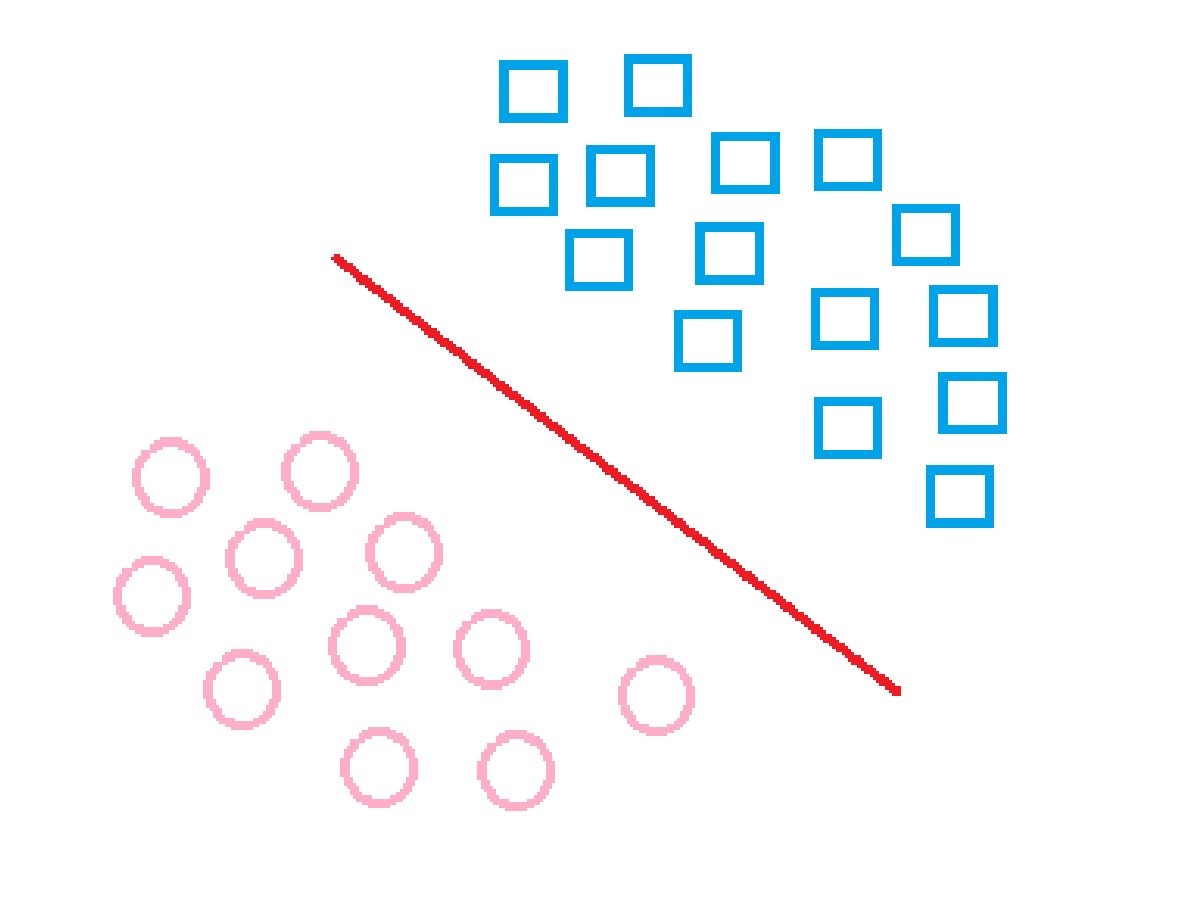
\includegraphics[width=0.5\linewidth]{svmEuclidSpace}
\caption{Illustration of the discriminant plane of SVM.}
\label{fig:svmEuclidSpace}
\end{figure}

\begin{equation}
\label{equ:svmOptimizationObjectFunction}
\begin{aligned}
&\mathop {\max }\limits_{w,b} \gamma \\
&s.t.\quad {d^{*i}} \ge \gamma,\quad i = 0,1,...,n - 1
\end{aligned}
\end{equation}
Where $\gamma$ is the minimum margin between all distances of data to the discriminant plane, $d^{*i}$ is the distance of $ith$ sample to discriminant plane.

Consider the label of data is either $-1$ or $1$, we can calculate the distance in unified type as shown in Eq.~\ref{equ:svmFunctionDistance}.

\begin{equation}
\label{equ:svmFunctionDistance}
{d^{*i}} = \frac{{{y^{*i}}\left( {{x^{*i}}w + b} \right)}}{{\parallel w\parallel }}
\end{equation}

The constraint of the optimization object function can be converted by Eq.~\ref{equ:svmConstraintConvert}.

\begin{equation}
\label{equ:svmConstraintConvert}
\begin{aligned}
&{d^{*i}} \ge \gamma ,i = 0,1,...,n - 1\\
 &\Rightarrow \frac{{{y^{*i}}\left( {{x^{*i}}w + b} \right)}}{{\parallel w\parallel }} \ge \gamma \\
 &\Rightarrow \frac{{{y^{*i}}\left( {{x^{*i}}w + b} \right)}}{{\parallel w\parallel }} \ge \frac{{{y^{*k}}\left( {{x^{*k}}w + b} \right)}}{{\parallel w\parallel }}\\
&let\quad  p = {y^{*k}}\left( {{x^{*k}}w + b} \right),p > 0,\tilde w = \frac{w}{p}, \tilde b = \frac{b}{p}\\
& \Rightarrow   \frac{{{y^{*k}}\left( {{x^{*k}}w + b} \right)}}{{\parallel w\parallel }} = \frac{p}{{\parallel w\parallel }} = \frac{1}{{\parallel \tilde w\parallel }}\\
& \Rightarrow \frac{{{y^{*i}}\left( {{x^{*i}}w + b} \right)}}{{\parallel w\parallel }} = \frac{{{y^{*i}}\left( {{x^{*i}}\tilde w + \tilde b} \right)}}{{\parallel \tilde w\parallel }} \ge \frac{1}{{\parallel \tilde w\parallel }} = \gamma 
\end{aligned}
\end{equation}
Where $p$ is always positive in linear separable problems, the distance of the $kth$ sample to discriminant plane is the minimum.


Then the optimization object function can be formalized as Eq.~\ref{equ:svmOOFConverted}.

\begin{equation}
\label{equ:svmOOFConverted}
\begin{aligned}
&\mathop {\max }\limits_{\tilde w} \frac{1}{{\parallel \tilde w\parallel }}\\
\sim &\mathop {\min }\limits_{\tilde w} \frac{1}{2}\parallel \tilde w{\parallel ^2}\\
s.t.\quad &{y^{*i}}\left( {{x^{*i}}\tilde w + \tilde b} \right) - 1 \ge 0 \quad i = 0,1,...,n - 1\\
\sim &1 - {y^{*i}}\left( {{x^{*i}}\tilde w + \tilde b} \right) \le 0,\quad i = 0,1,...,n - 1
\end{aligned}
\end{equation}

Because the $\tilde w$ and $\tilde b$ are both the linear relation to $w$ and $b$, so the discriminant function can be written as Eq.~\ref{equ:svmDiscriminantFunctionConverted}.

\begin{equation}
\label{equ:svmDiscriminantFunctionConverted}
l = g\left(x \right) = x\tilde w + \tilde b > 0?1: - 1
\end{equation} 

In linear separable problem, the training samples which are the most closed to the discriminant plane are the support vectors. The maximum margin of training samples to discriminant plane is $\frac{1}{\tilde{w}}$. Fig.\ref{fig:svmSupportVector} illustrate the support vectors and margin. From the picture, we can find that the SVM is determined by a small part of important training samples.

\begin{figure}
\centering
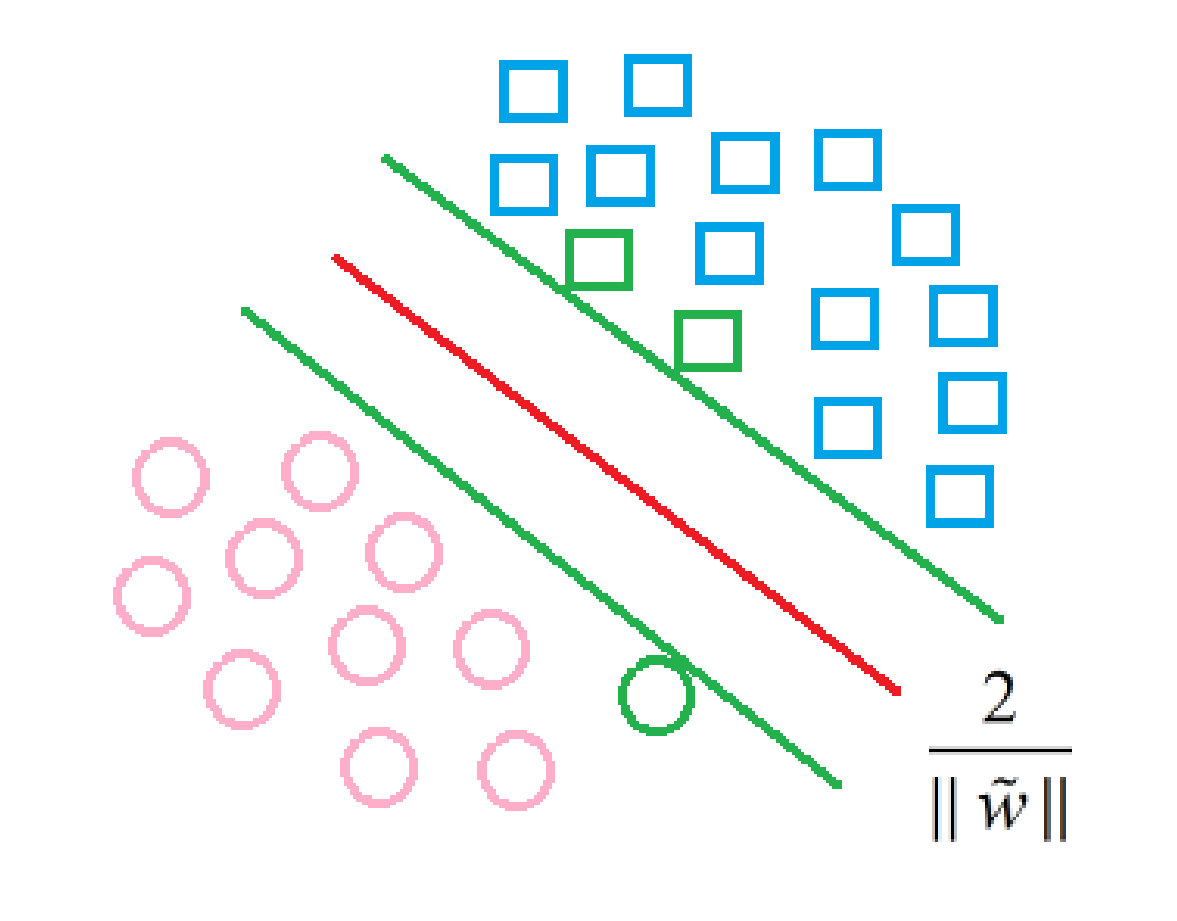
\includegraphics[width=0.5\linewidth]{svmSupportVector}
\caption{Illustration of the support vectors and margin in SVM. The red line denotes the discriminant plane and the green lines denote the margin boundary plane. The samples marked as green color are the support vectors.}
\label{fig:svmSupportVector}
\end{figure}

On the basis of the sufficient conditions of KKT, the value which satisfy the conditions in following Eq.~\ref{equ:svmOptimizationSolutionConditions} are the optimization solution.

\begin{equation}
\label{equ:svmOptimizationSolutionConditions}
\begin{aligned}
&\left\{ {\begin{array}{*{20}{c}}
{f\left( {\tilde w,\tilde b} \right) = \frac{1}{2}\parallel \tilde w{\parallel ^2} = \frac{1}{2}\tilde w{{\tilde w}^t}}\\
{{g^{*i}}\left( {\tilde w,\tilde b} \right) = 1 - {y^{*i}}\left( {{x^{*i}}\tilde w + \tilde b} \right)}
\end{array}} \right.\\
 \to &\left\{ {\begin{array}{*{20}{c}}
{{g^{*i}}\left( {\tilde w,\tilde b} \right) \le 0,{u^{*i}} \ge 0,{u^{*i}}{g^{*i}}\left( {\tilde w,\tilde b} \right) = 0,i = 0,1,...l - 1}\\
{\frac{{\partial f\left( {\tilde w,\tilde b} \right)}}{{\partial \tilde w}} = 0}\\
{\frac{{\partial f\left( {\tilde w,\tilde b} \right)}}{{\partial \tilde b}} = 0}
\end{array}} \right.\\
 \Rightarrow &\left\{ {\begin{array}{*{20}{c}}
{{g^{*i}}\left( {\tilde w,\tilde b} \right) \le 0,{u^{*i}} \ge 0,{u^{*i}}{g^{*i}}\left( {\tilde w,\tilde b} \right) = 0,i = 0,1,...l - 1}\\
{\tilde w = \sum\limits_{i = 0}^{l - 1} {{u^{*i}}{y^{*i}}{{\left( {{x^{*i}}} \right)}^t}} }\\
{\sum\limits_{i = 0}^{l - 1} {{u^{*i}}{y^{*i}}}  = 0}
\end{array}} \right.
\end{aligned}
\end{equation}

However, we can't directly acquire the optimization solution by solving the conditions. Thus we adopt a two-step way by adopting the Lagrange multiplier method. We formalize the Lagrange multiplier by the Eq.~\ref{equ:svmLagrangeMultiplier}.

\begin{equation}
\label{equ:svmLagrangeMultiplier}
\begin{aligned}
L\left( {\tilde w,\tilde b,u} \right) &= \frac{1}{2}\parallel \tilde w{\parallel ^2} + \sum\limits_{i = 0}^{n - 1} {{u^{*i}}\left( {1 - {y^{*i}}\left( {{x^{*i}}\tilde w + \tilde b} \right)} \right)} \\
 &= \frac{1}{2}\parallel \tilde w{\parallel ^2} - \sum\limits_{i = 0}^{n - 1} {{u^{*i}}{y^{*i}}\left( {{x^{*i}}\tilde w + \tilde b} \right)}  + \sum\limits_{i = 0}^{n - 1} {{u^{*i}}} 
\end{aligned}
\end{equation}

The optimization object can be described as Eq.~\ref{equ:svmLagrangeOO}.

\begin{equation}
\label{equ:svmLagrangeOO}
\mathop {\min }\limits_{\tilde w,\tilde b} \mathop {\max }\limits_u L\left( {\tilde w,\tilde b,u} \right) = \mathop {\min }\limits_{\tilde w,\tilde b} \mathop {\max }\limits_u \frac{1}{2}\parallel \tilde w{\parallel ^2} - \sum\limits_{i = 0}^{n - 1} {{u^{*i}}{y^{*i}}\left( {{x^{*i}}\tilde w + \tilde b} \right)}  + \sum\limits_{i = 0}^{n - 1} {{u^{*i}}}
\end{equation}

We first calculate the point of maximum value (${\hat u}$) through making the derivation of $L$ about $u$ to zero. The computation process can be described as Eq.~\ref{equ:svmOriginalMaximumU}.

\begin{equation}
\label{equ:svmOriginalMaximumU}
\begin{aligned}
&\frac{{\partial L\left( {\tilde w,\tilde b,u} \right)}}{{\partial {u^{*i}}}} =  - {y^{*i}}\left( {{x^{*i}}\tilde w + \tilde b} \right) + 1 = 0\\
&\Rightarrow {y^{*i}}\left( {{x^{*i}}\tilde w + \tilde b} \right) = 1
\end{aligned}
\end{equation}

Then the original problem can be converted to Eq.~\ref{equ:svmConvertedFromOriginal}.

\begin{equation}
\label{equ:svmConvertedFromOriginal}
\begin{aligned}
&\mathop {\min }\limits_{\tilde w,\tilde b} \mathop {\max }\limits_u L\left( {\tilde w,\tilde b,u} \right) = \mathop {\min }\limits_{\tilde w,\tilde b} \frac{1}{2}\parallel \tilde w{\parallel ^2}\\
&s.t.\quad {y^{*i}}\left( {{x^{*i}}\tilde w + \tilde b} \right) = 1,i = 0,1,...,n - 1
\end{aligned}
\end{equation} 

However, the constraint conditions can not be satisfied in most times due to the variation of training data in feature space (if we want to satisfy the constraint conditions, then the training data need has exhaustively same true and false samples in feature space respectively. In order word, the training data can be considered only has two samples, one for true category and one for false category). Here we sick in a difficult position so that we can't solve the optimization object of SVM.

Fortunately, we can convert the original problem to dual problem (the original and dual problems are equivalent, as described in Sec.\ref{sec:kktSufficientConditions}), and find a way to solve it. Specifically, the dual problem for the original problem can be described in Eq.~\ref{equ:svmLagrangeDualOO}.

\begin{equation}
\label{equ:svmLagrangeDualOO}
\mathop {\max }\limits_u \mathop {\min }\limits_{\tilde w,\tilde b} L\left( {\tilde w,\tilde b,u} \right) = \mathop {\max }\limits_u \mathop {\min }\limits_{\tilde w,\tilde b} \frac{1}{2}\parallel \tilde w{\parallel ^2} - \sum\limits_{i = 0}^{n - 1} {{u^{*i}}{y^{*i}}\left( {{x^{*i}}\tilde w + \tilde b} \right)}  + \sum\limits_{i = 0}^{n - 1} {{u^{*i}}} 
\end{equation}

We first calculate the point of minimum value (${\hat w}, {\hat b}$) through making the derivation of $L$ about ${\tilde w}$ and $\tilde b$ to zero respectively. The computation process can be described as Eq.~\ref{equ:svmDualMinimumWB}.

\begin{equation}
\label{equ:svmDualMinimumWB}
\begin{aligned}
&\frac{{\partial L}}{{\partial \tilde w}} = \tilde w - \sum\limits_{i = 0}^{n - 1} {{u^{*i}}{y^{*i}}{{\left( {{x^{*i}}} \right)}^t}}  = 0\\
& \Rightarrow \tilde w = \sum\limits_{i = 0}^{n - 1} {{u^{*i}}{y^{*i}}{{\left( {{x^{*i}}} \right)}^t}} \\
&\frac{{\partial L}}{{\partial \tilde b}} = \sum\limits_{i = 0}^{n - 1} {{u^{*i}}{y^{*i}}}  = 0
\end{aligned}
\end{equation}

Then the dual problem can be converted to Eq.~\ref{equ:svmConvertedFromDual}.

\begin{equation}
\label{equ:svmConvertedFromDual}
\begin{aligned}
\mathop {\min }\limits_{\tilde w,\tilde b} L\left( {\tilde w,\tilde b,u} \right) &= \frac{1}{2}\parallel \sum\limits_{i = 0}^{n - 1} {{u^{*i}}{y^{*i}}{{\left( {{x^{*i}}} \right)}^t}} {\parallel ^2} \\
&-\sum\limits_{i = 0}^{n - 1} {{u^{*i}}{y^{*i}}\left( {{x^{*i}}\left( {\sum\limits_{j = 0}^{n - 1} {{u^{*j}}{y^{*j}}{{\left( {{x^{*j}}} \right)}^t}} } \right) + \tilde b} \right)}  + \sum\limits_{i = 0}^{n - 1} {{u^{*i}}} \\
= \frac{1}{2}\parallel \sum\limits_{i = 0}^{n - 1} &{{u^{*i}}{y^{*i}}{x^{*i}}} {\parallel ^2} - \sum\limits_{i = 0}^{n - 1} {\sum\limits_{j = 0}^{n - 1} {{u^{*i}}{u^{*j}}{y^{*i}}{y^{*j}}\left( {{x^{*i}} \cdot {x^{*j}}} \right)} } + \sum\limits_{i = 0}^{n - 1} {{u^{*i}}} \\
\because\ \parallel \sum\limits_{i = 0}^{n - 1} {{v^{*i}}} {\parallel ^2},&\quad {\left(\rm{v\ is\ a\ vector}\right)}\\
 =& \parallel {v^{*0}} + ... + {v^{*n - 1}}{\parallel ^2}\\
 =& \parallel \left( {{v_0}^{*0} + ... + {v_0}^{*n - 1},...,{v_{d - 1}}^{*0} + ... + {v_{d - 1}}^{*n - 1}} \right){\parallel ^2}\\
 =& {\left( {{v_0}^{*0} + ... + {v_0}^{*n - 1}} \right)^2} + ... + {\left( {{v_{d - 1}}^{*0} + ... + {v_{d - 1}}^{*n - 1}} \right)^2}\\
 =& \sum\limits_{k = 0}^{d - 1} {\sum\limits_{i = 0}^{n - 1} {\sum\limits_{j = 0}^{n - 1} {{v_k}^{*i}{v_k}^{*j}} } } \\
 =& \sum\limits_{i = 0}^{n - 1} {\sum\limits_{j = 0}^{n - 1} {\sum\limits_{k = 0}^{d - 1} {{v_k}^{*i}{v_k}^{*j}} } } \\
 =& \sum\limits_{i = 0}^{n - 1} {\sum\limits_{j = 0}^{n - 1} {{v^{*i}} \cdot {v^{*j}}} } \\
\therefore\ \frac{1}{2}\parallel \sum\limits_{i = 0}^{n - 1} {{u^{*i}}{y^{*i}}{x^{*i}}} {\parallel ^2} &= \frac{1}{2}\sum\limits_{i = 0}^{n - 1} {\sum\limits_{j = 0}^{n - 1} {\left( {{u^{*i}}{y^{*i}}{x^{*i}}} \right) \cdot \left( {{u^{*j}}{y^{*j}}{x^{*j}}} \right)} } \\
 &= \frac{1}{2}\sum\limits_{i = 0}^{n - 1} {\sum\limits_{j = 0}^{n - 1} {{u^{*i}}{u^{*j}}{y^{*i}}{y^{*j}}\left( {{x^{*i}} \cdot {x^{*j}}} \right)} } \\
\therefore \mathop {\min }\limits_{\tilde w,\tilde b} L\left( {\tilde w,\tilde b,u} \right) &=  - \frac{1}{2}\sum\limits_{i = 0}^{n - 1} {\sum\limits_{j = 0}^{n - 1} {{u^{*i}}{u^{*j}}{y^{*i}}{y^{*j}}\left( {{x^{*i}} \cdot {x^{*j}}} \right)} }  + \sum\limits_{i = 0}^{n - 1} {{u^{*i}}} 
\end{aligned}
\end{equation}

Thus the optimization object function is shown in Eq.~\ref{equ:svmLinearSVMForLinearProblem}.
   
\begin{equation}
\label{equ:svmLinearSVMForLinearProblem}
\begin{aligned}
&\mathop {\max }\limits_u  - \frac{1}{2}\sum\limits_{i = 0}^{n - 1} {\sum\limits_{j = 0}^{n - 1} {{u^{*i}}{u^{*j}}{y^{*i}}{y^{*j}}\left( {{x^{*i}} \cdot {x^{*j}}} \right)} }  + \sum\limits_{i = 0}^{n - 1} {{u^{*i}}} \\
 \sim &\mathop {\min }\limits_u \frac{1}{2}\sum\limits_{i = 0}^{n - 1} {\sum\limits_{j = 0}^{n - 1} {{u^{*i}}{u^{*j}}{y^{*i}}{y^{*j}}\left( {{x^{*i}} \cdot {x^{*j}}} \right)} }  - \sum\limits_{i = 0}^{n - 1} {{u^{*i}}} \\
s.t.\ &\sum\limits_{i = 0}^{n - 1} {{u^{*i}}{y^{*i}}}  = 0\\
&{u^{*i}} \ge 0,\ i = 0,1,...,n - 1
\end{aligned}
\end{equation}

\subsection{Soft Margin SVM}
For an approximate linear separable problem, it is very likely to be essentially linear separable while contains some noise samples in training data, as shown in Fig.\ref{fig:svmNoiseSamplesInApproximateLinear}. We can not directly exploit the hard margin SVM due to the constraint is unsatisfied in Eq.~\ref{equ:svmConstraintConvert} (the distance may be negative or zero).

\begin{figure}
\centering
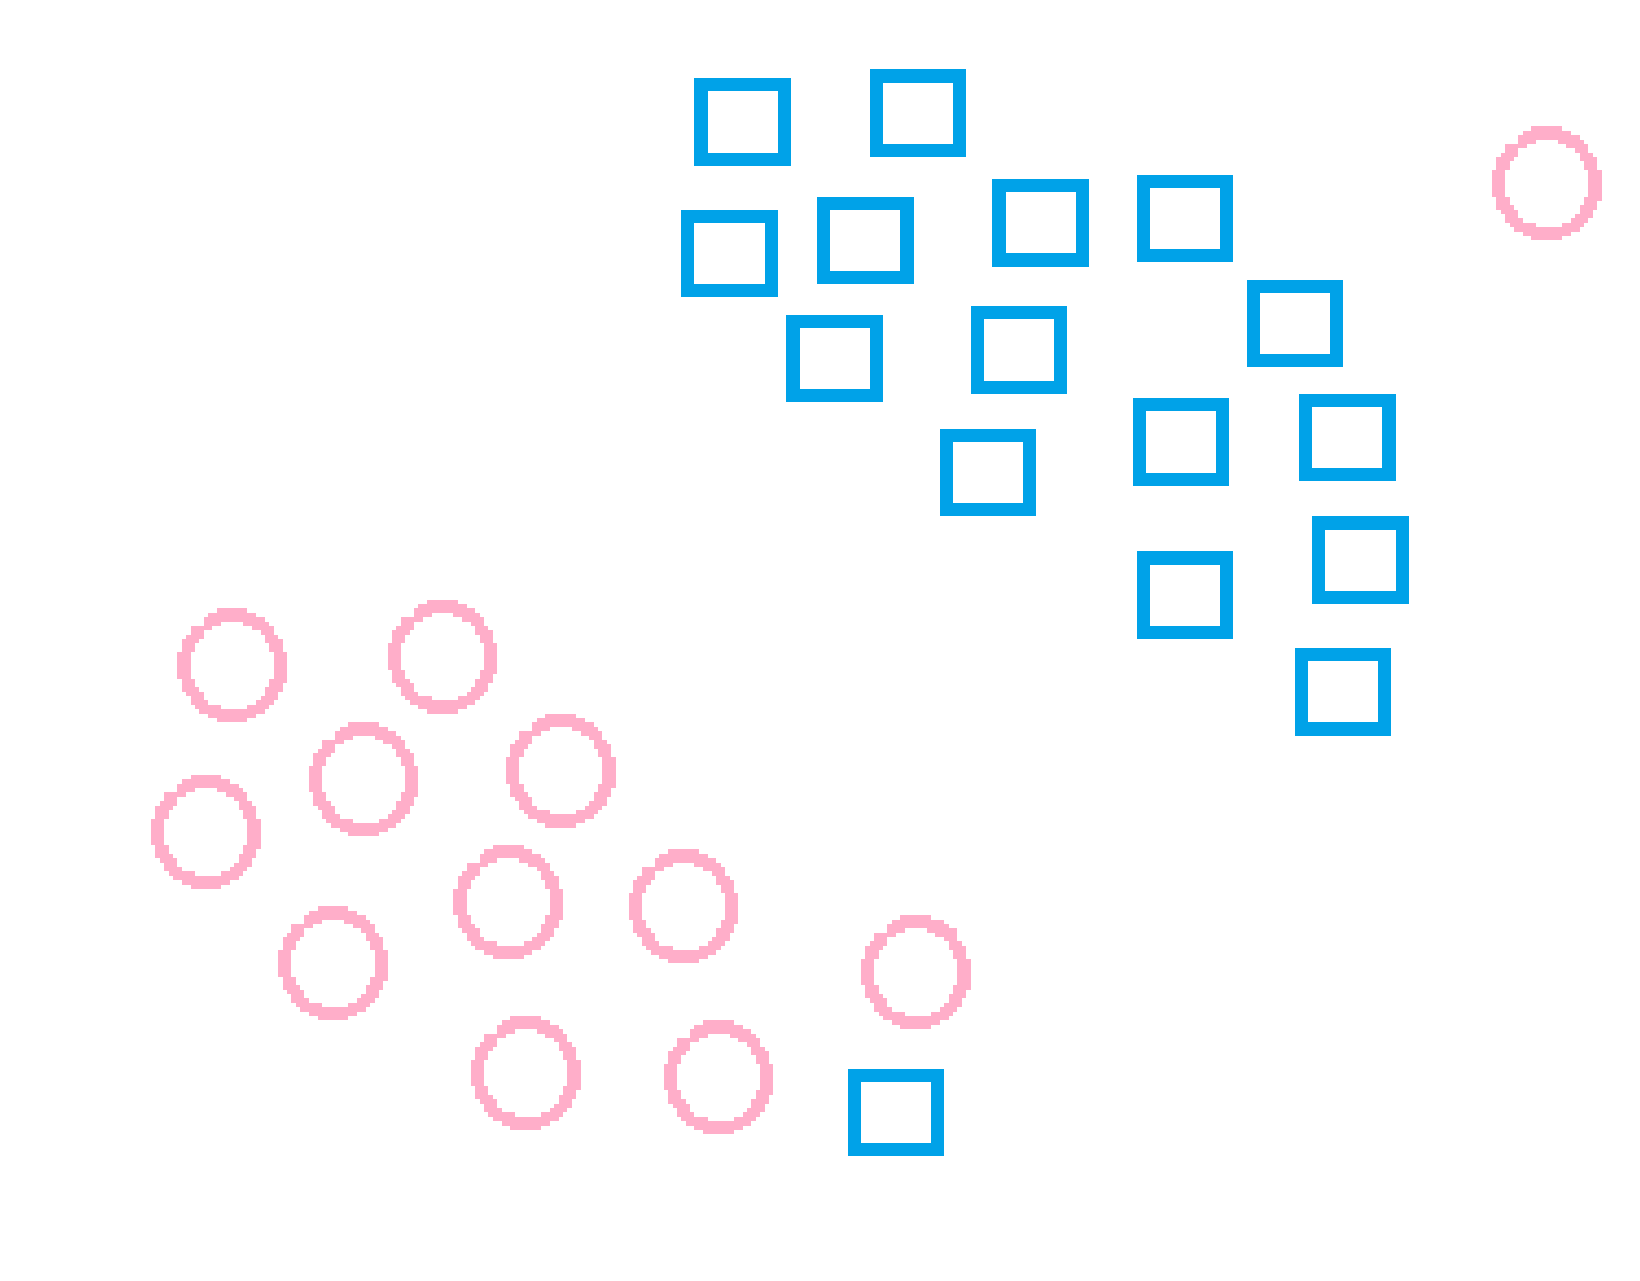
\includegraphics[width=0.5\linewidth]{svmNoiseSamplesInApproximateLinear}
\caption{Illustration of an approximate linear separable problem.}
\label{fig:svmNoiseSamplesInApproximateLinear}
\end{figure}

To learn a desired discriminant plane, we apply the soft margin to SVM by change the constraint in Eq.~\ref{equ:svmConstraintConvert}. We assign a distance bias $\varepsilon \left(\varepsilon \ge 0\right)$ that can make every distance be positive as defined in Eq.~\ref{equ:svmSoftDistance}. In other words, appending bias can be considered as a bias transform that transform the original training data from approximate linear separable state to linear separable state. 

\begin{equation}
\label{equ:svmSoftDistance}
{d^{*i}} = \frac{{{y^{*i}}\left( {{x^{*i}}w + b} \right) + {\varepsilon ^{*i}}}}{{\parallel w\parallel }} > 0,\quad \left(\varepsilon \ge 0\right)
\end{equation}

Then the constraint defined by Eq.~\ref{equ:svmConstraintConvert} can be described as Eq.~\ref{equ:svmSoftConstraintConvert}.

\begin{equation}
\label{equ:svmSoftConstraintConvert}
\begin{aligned}
&{d^{*i}} \ge \gamma ,i = 0,1,...,n - 1\\
 &\Rightarrow \frac{{{y^{*i}}\left( {{x^{*i}}w + b} \right) + {\varepsilon ^{*i}}}}{{\parallel w\parallel }} \ge \frac{{{y^{*k}}\left( {{x^{*k}}w + b} \right) + {\varepsilon ^{*k}}}}{{\parallel w\parallel }}\\
&let\ p = {y^{*k}}\left( {{x^{*k}}w + b} \right) + {\varepsilon ^{*k}},\ p > 0,\ \tilde w = \frac{w}{p},\ \tilde b = \frac{b}{p},\ {{\tilde \varepsilon }^{*i}} = \frac{{{\varepsilon ^{*i}}}}{p}\\
 &\Rightarrow \frac{{{y^{*i}}\left( {{x^{*i}}w + b} \right) + {\varepsilon ^{*i}}}}{{\parallel w\parallel }} = \frac{{{y^{*i}}\left( {{x^{*i}}\tilde w + \tilde b} \right) + {{\tilde \varepsilon }^{*i}}}}{{\parallel \tilde w\parallel }} \ge \frac{1}{{\parallel \tilde w\parallel }}\\
 &\Rightarrow {y^{*i}}\left( {{x^{*i}}\tilde w + \tilde b} \right) + {{\tilde \varepsilon }^{*i}} \ge 1
\end{aligned}
\end{equation}

Obviously, in order to keep the majority properties, the transformational degree should not be so acute, that is to say, the sum of all bias of training samples should not be very large. So we add a penalty term by employing the penalty factor $c$ for the optimization object function as shown in Eq.~\ref{equ:svmSoftOOF}.

\begin{equation}
\label{equ:svmSoftOOF}
\begin{aligned}
&\mathop {\min }\limits_{\tilde w} \frac{1}{2}\parallel \tilde w{\parallel ^2} + c \sum\limits_{i = 0}^{n - 1} {{{\tilde \varepsilon }^{*i}}} \\
s.t.\quad &1 - {y^{*i}}\left( {{x^{*i}}\tilde w + \tilde b} \right) - {{\tilde \varepsilon }^{*i}} \le 0,\quad {{\tilde \varepsilon }^{*i}} \ge 0,\quad i = 0,1,...,n - 1
\end{aligned}
\end{equation}

If ${{\tilde \varepsilon }^{*i}} = 0$, then $ith$ sample is on or far away from the margin boundary. If ${{\tilde \varepsilon }^{*i}} > 0$, then $ith$ sample cross the margin boundary and after transform the sample will be on the margin boundary (thus the distance of this sample to the corresponding margin boundary is $\frac{{{{\tilde \varepsilon }^{*i}}}}{{\parallel \tilde w\parallel }}$), as illustrated in Fig.\ref{fig:svmSoftDistance}. The very large penalty factor $c$ make the sum of bias very small while the very small penalty factor make the margin between the two margin boundaries very large, as illustrated in Fig.\ref{fig:svmSoftPenaltyEffect}.

\begin{figure}
\centering
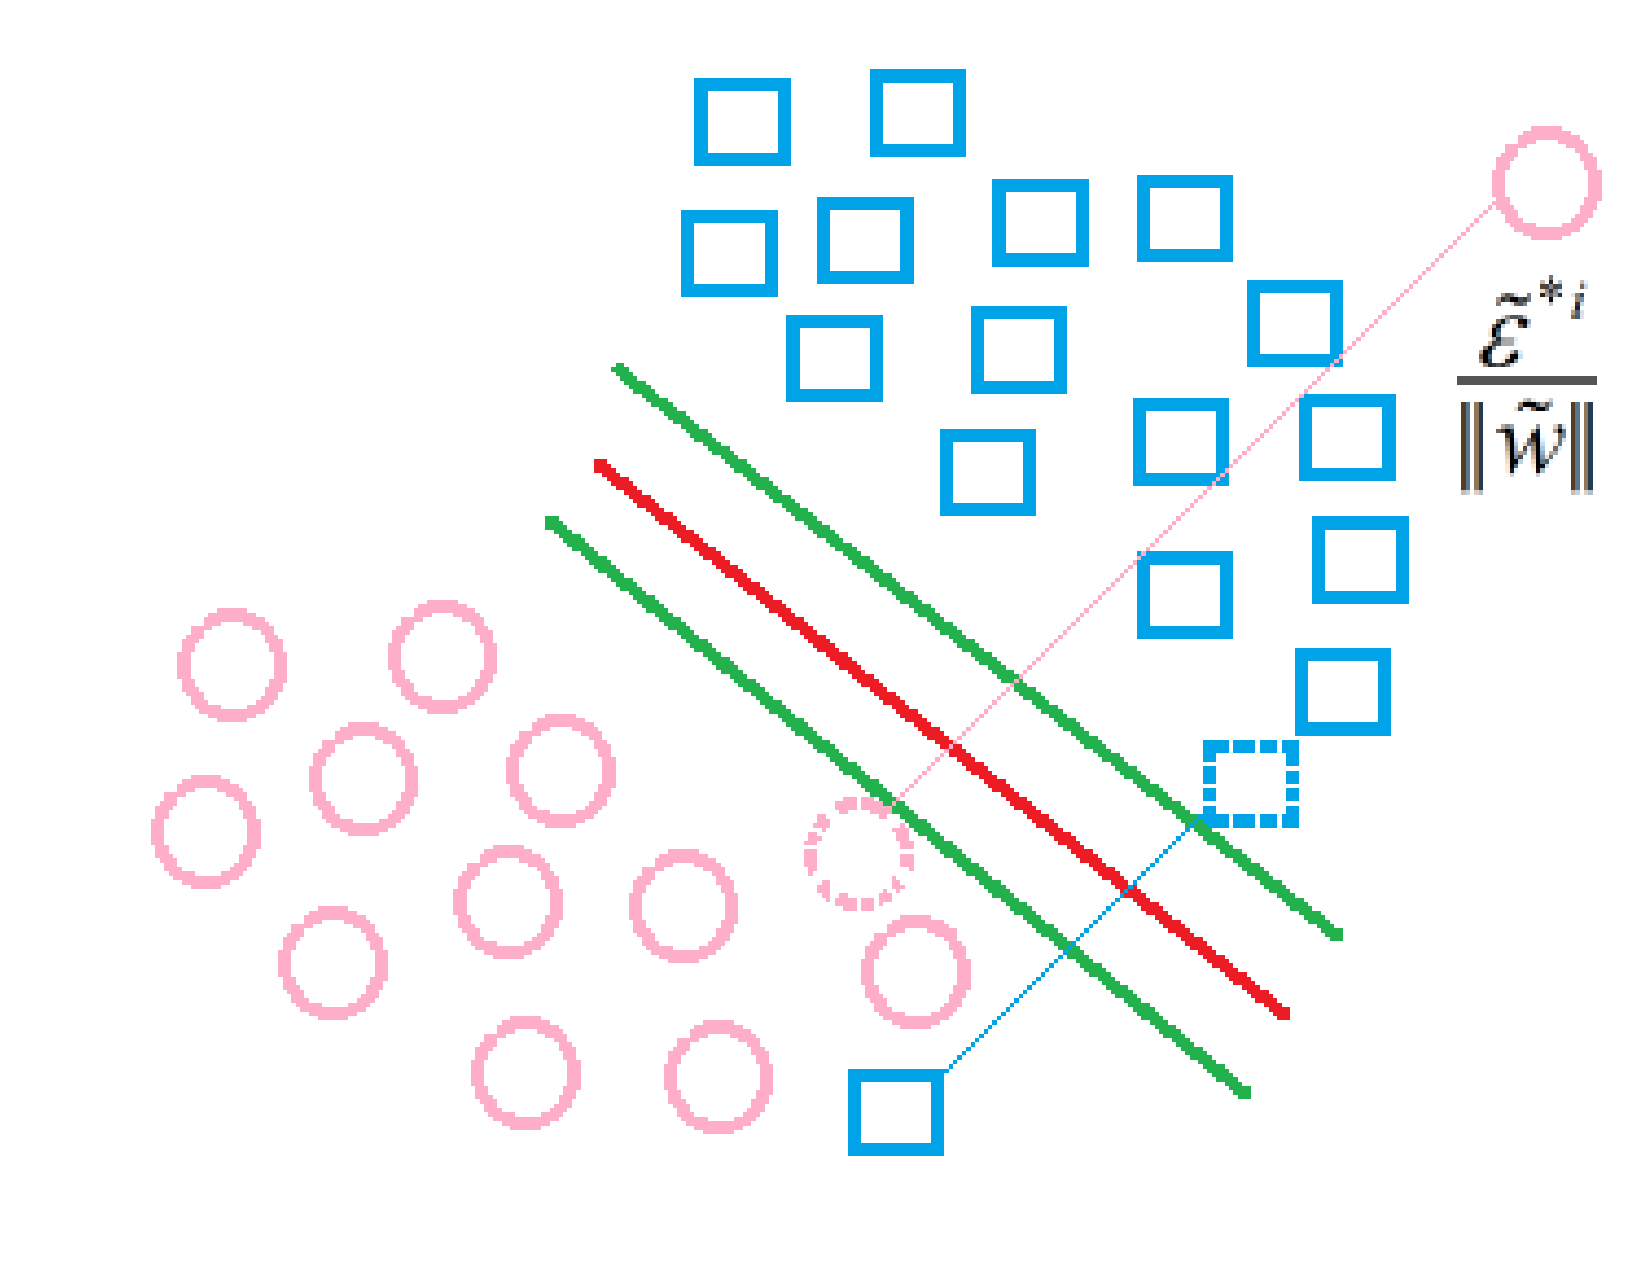
\includegraphics[width=0.5\linewidth]{svmSoftDistance}
\caption{Illustration of the bias transform.}
\label{fig:svmSoftDistance}
\end{figure}

\begin{figure}
\centering
\subfigure[]{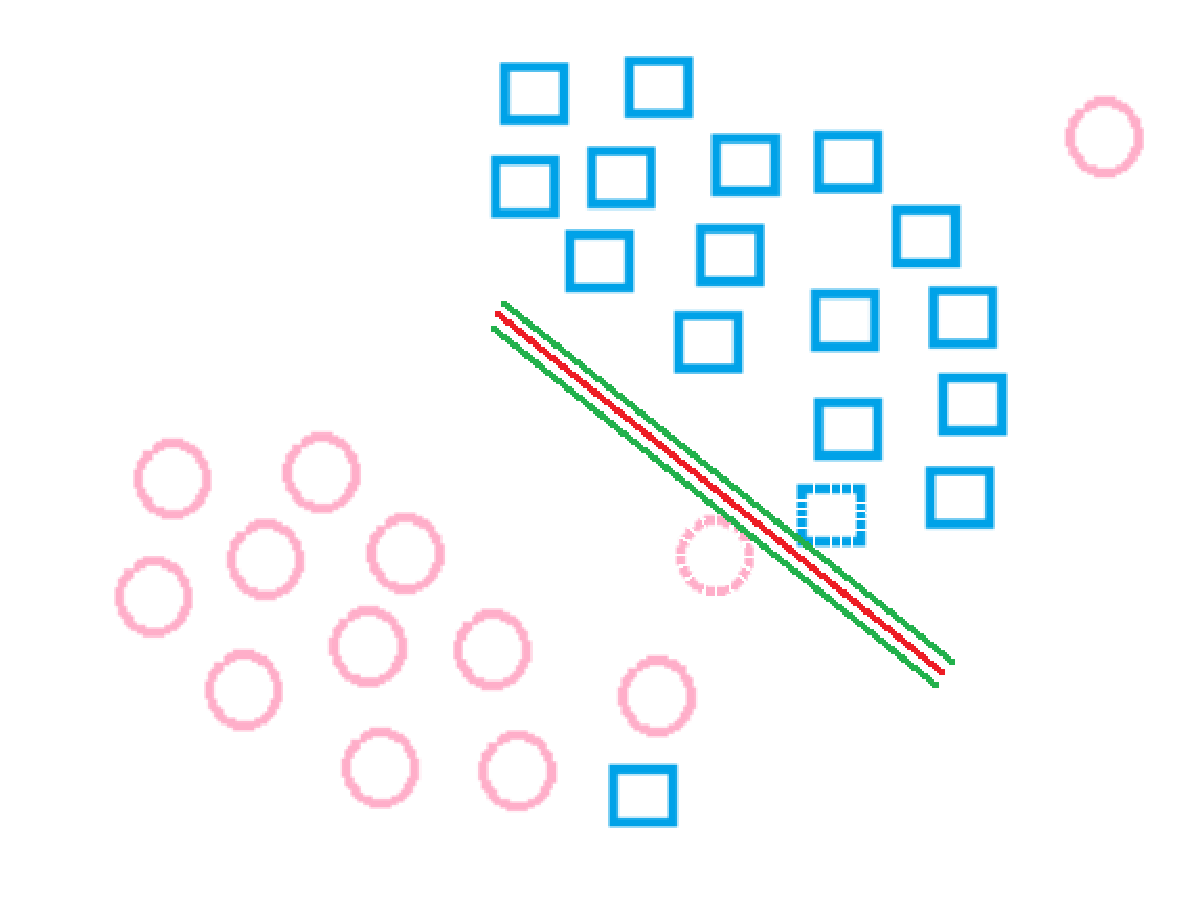
\includegraphics[width=0.45\linewidth]{svmSoftLargePenalty}}
\subfigure[]{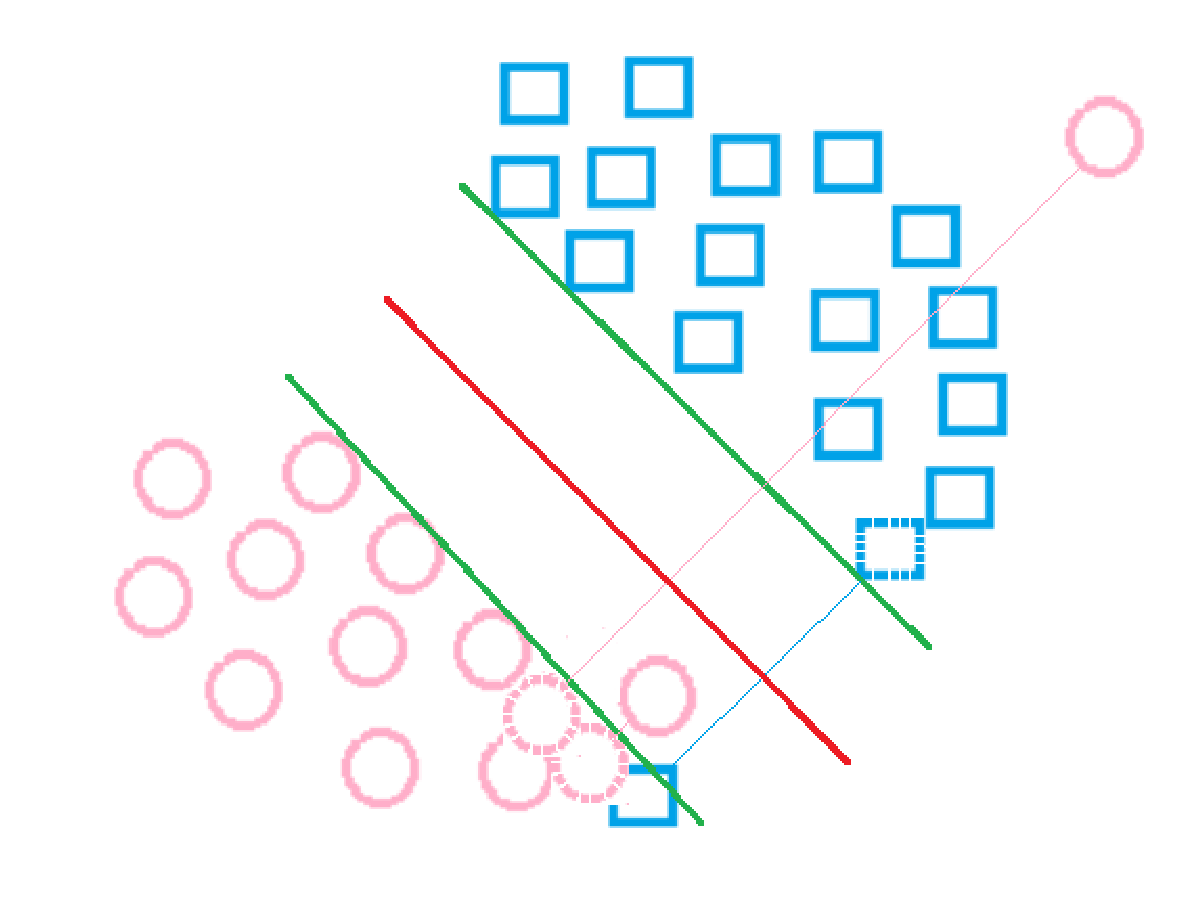
\includegraphics[width=0.45\linewidth]{svmSoftSmallPenalty}}
\caption{Illustration of the effect by employing different scale of penalty factors. (a) employs the large penalty factor, thus the bias of samples are very small and the margin between two margin boundaries is very small. (b) employs the small penalty factor so that both the margin and the bias are very large.}
\label{fig:svmSoftPenaltyEffect}
\end{figure}


The original and dual Lagrange Multipliers are defined as Eq.~\ref{equ:svmSoftLagrangeMultipliers}.

\begin{equation}
\label{equ:svmSoftLagrangeMultipliers}
\begin{aligned}
&\mathop {\min }\limits_{\tilde w,\tilde b,\tilde \varepsilon } \mathop {\max }\limits_u L\left( {\tilde w,\tilde b,u} \right) = \mathop {\min }\limits_{\tilde w,\tilde b,\tilde \varepsilon } \mathop {\max }\limits_u \frac{1}{2}\parallel \tilde w{\parallel ^2} \\
&+ \sum\limits_{i = 0}^{n - 1} {{u^{*i}}\left( {1 - {y^{*i}}\left( {{x^{*i}}\tilde w + \tilde b} \right) - {{\tilde \varepsilon }^{*i}}} \right)}  + c\sum\limits_{i = 0}^{n - 1} {{{\tilde \varepsilon }^{*i}}}  - \sum\limits_{i = 0}^{n - 1} {{v^{*i}}{{\tilde \varepsilon }^{*i}}} \\
 \sim &\mathop {\max }\limits_u \mathop {\min }\limits_{\tilde w,\tilde b,\tilde \varepsilon } L\left( {\tilde w,\tilde b,u} \right) = \mathop {\max }\limits_u \mathop {\min }\limits_{\tilde w,\tilde b,\tilde \varepsilon } \frac{1}{2}\parallel \tilde w{\parallel ^2} - \sum\limits_{i = 0}^{n - 1} {{u^{*i}}{y^{*i}}\left( {{x^{*i}}\tilde w + \tilde b} \right)}  + \sum\limits_{i = 0}^{n - 1} {{u^{*i}}} \\
 & - \sum\limits_{i = 0}^{n - 1} {{u^{*i}}{{\tilde \varepsilon }^{*i}}}  + c\sum\limits_{i = 0}^{n - 1} {{{\tilde \varepsilon }^{*i}}}  - \sum\limits_{i = 0}^{n - 1} {{v^{*i}}{{\tilde \varepsilon }^{*i}}} \\
s.t.\ &{u^{*i}} \ge 0,{v^{*i}} \ge 0,\quad i = 0,1,...,n - 1
\end{aligned}
\end{equation}

The simplification process as shown in Eq.~\ref{equ:svmSoftSimplificationOOF}. Then we get the final optimization object function.

\begin{equation}
\label{equ:svmSoftSimplificationOOF}
\begin{aligned}
&\left\{ {\begin{array}{*{20}{c}}
{\frac{{\partial L}}{{\partial \tilde w}} = \tilde w - \sum\limits_{i = 0}^{n - 1} {{u^{*i}}{y^{*i}}{{\left( {{x^{*i}}} \right)}^t}}  = 0}\\
{\frac{{\partial L}}{{\partial \tilde b}} =  - \sum\limits_{i = 0}^{n - 1} {{u^{*i}}{y^{*i}}}  = 0}\\
{\frac{{\partial L}}{{\partial {{\tilde \varepsilon }^i}}} =  - {u^{*i}} + c - {v^{*i}} = 0}
\end{array}} \right.\\
 \Rightarrow &\mathop {\max }\limits_u \mathop {\min }\limits_{\tilde w,\tilde b,\tilde \varepsilon } L\left( {\tilde w,\tilde b,u} \right) = \mathop {\max }\limits_u  - \frac{1}{2}\sum\limits_{i = 0}^{n - 1} {\sum\limits_{j = 0}^{n - 1} {{u^{*i}}{u^{*j}}{y^{*i}}{y^{*j}}\left( {{x^{*i}} \cdot {x^{*j}}} \right) + } } \sum\limits_{i = 0}^{n - 1} {{u^{*i}}} \\
 \sim &\mathop {\min }\limits_u \frac{1}{2}\sum\limits_{i = 0}^{n - 1} {\sum\limits_{j = 0}^{n - 1} {{u^{*i}}{u^{*j}}{y^{*i}}{y^{*j}}\left( {{x^{*i}} \cdot {x^{*j}}} \right) - } } \sum\limits_{i = 0}^{n - 1} {{u^{*i}}} \\
s.t.\ &\sum\limits_{i = 0}^{n - 1} {{u^{*i}}{y^{*i}}}  = 0\\
&c = {u^{*i}} + {v^{*i}},{u^{*i}} \ge 0,{v^{*i}} \ge 0,i = 0,1,...,n - 1\\
 \sim\ &0 \le {u^{*i}} \le c,i = 0,1,...,n - 1
\end{aligned}
\end{equation}

\chapter{Bayes Based Models}
\chapter{Decision Tree Based Models}

\section{Over-fitting}
For a perfect training data as the same described in Sec.\ref{sec:overFittingInDR}, if we want to learn it successfully using the decision tree based model, we need to extract as many as possible features for our learning model. 
It is very different from the DR based model since the the ability for fitting training data in decision tree based models is the number of rules (more features, we can make more rules) while the ability is the number of parameters in DR based models (more parameters, we can acquire a more complex DR based models). 
The decision boundary of decision tree is criss-crossed in feature space as shown in Fig.\ref{fig:overFittingDiscriminantCurveInDecisionTree}. 

\begin{figure}
\centering
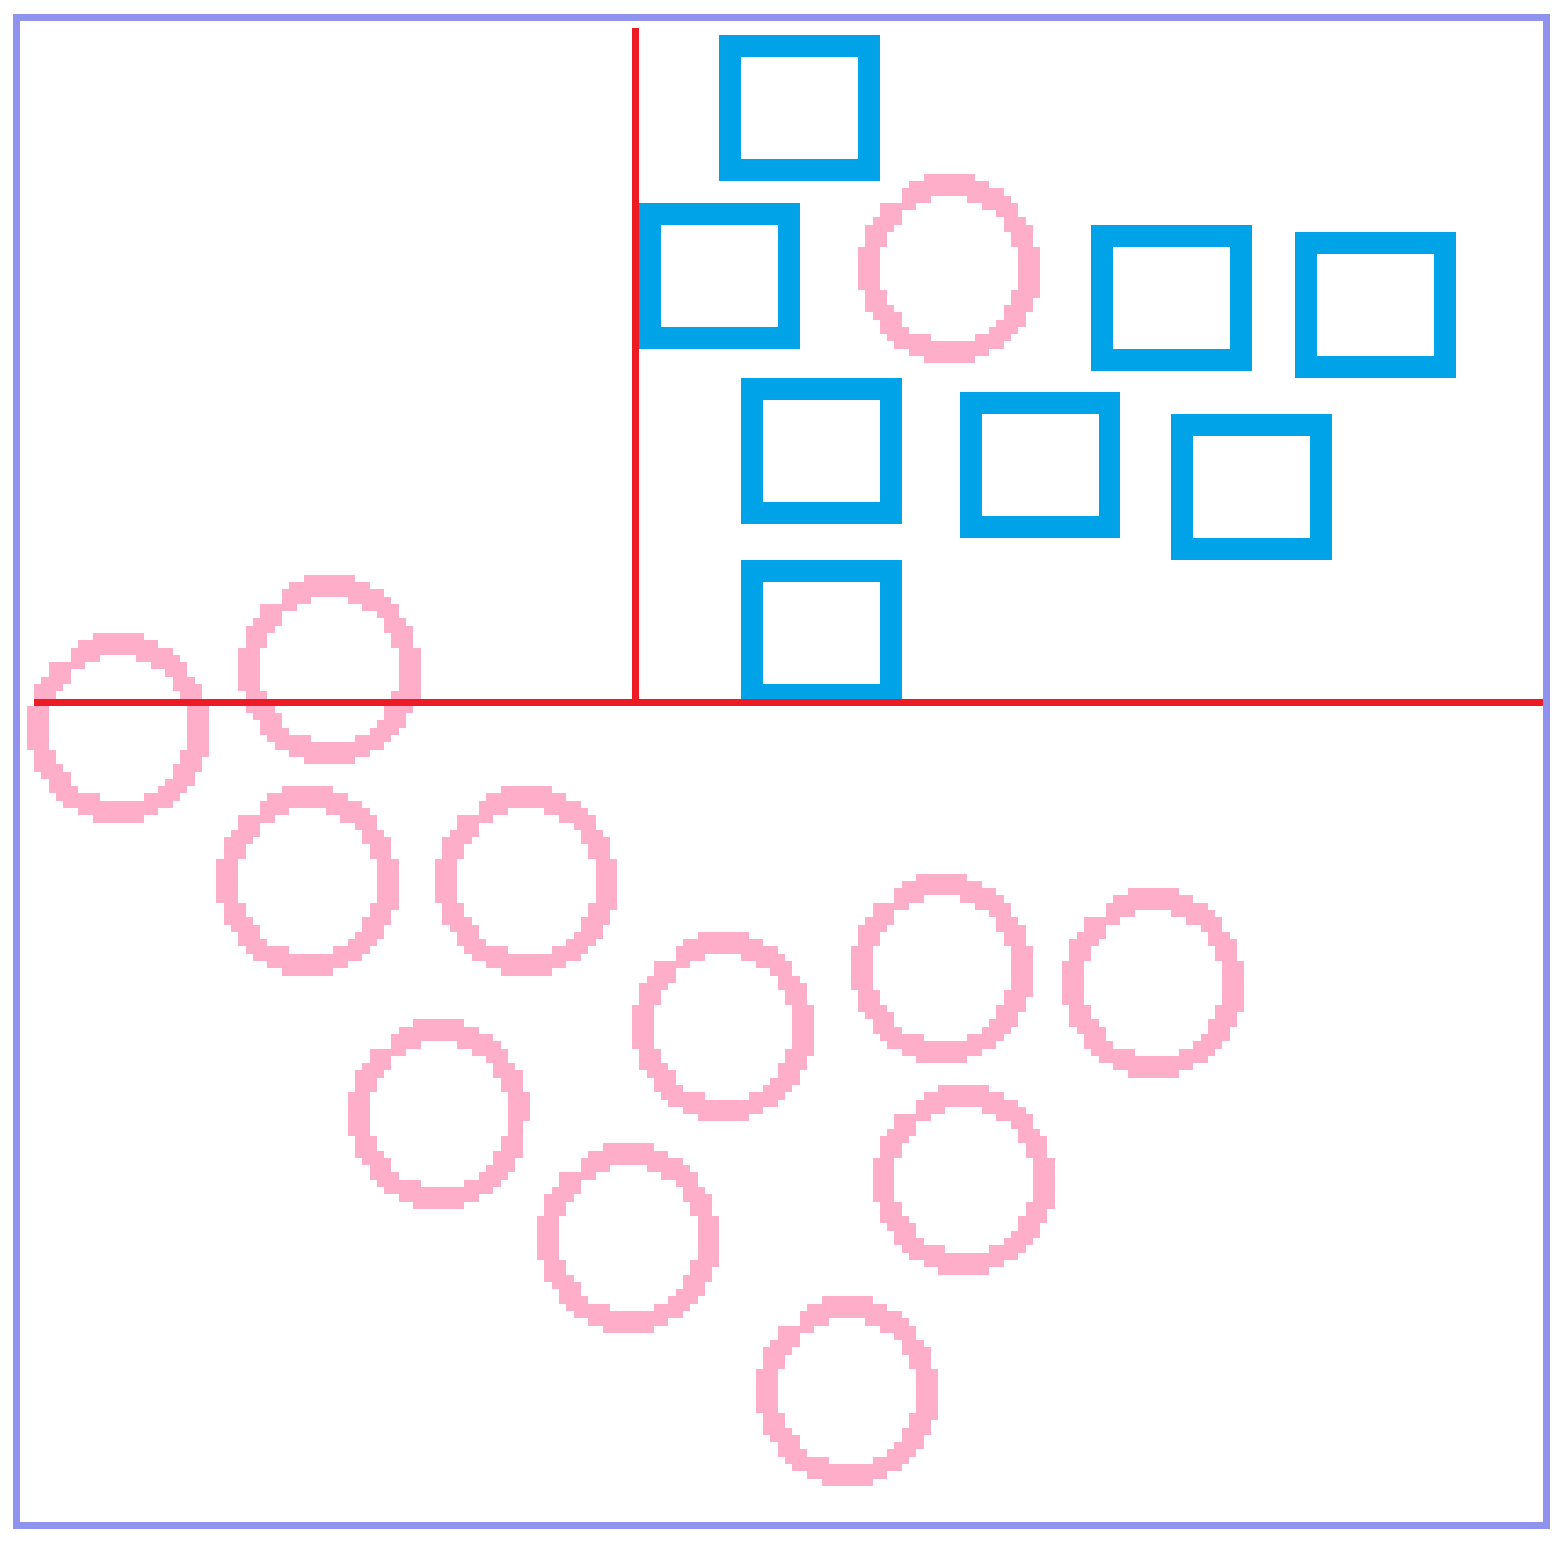
\includegraphics[width=0.5\linewidth]{overFittingDiscriminantCurveInDecisionTree}
\caption{Illustration of the decision boundary in decision tree.}
\label{fig:overFittingDiscriminantCurveInDecisionTree}
\end{figure}

In imperfect training data, the noises may affect incorrectly the DR curve by the rules and the influence of insufficiency of data will be amplified in deep layers since the features are weakly partitive ability and the samples are few in the deep layers of decision trees. So the direct way to avoid the situation is to limit the depth of the decision tree, such as setting the maximum depth, early stopping division and applying pruning (in random forest or adaboost model, the pruning can be ignored due to the complexity of the operation). Reducing such useless features can also reduce the complexity of the DR curve in decision tree model.

\section{Decision Tree}

\section{Random Tree and Forest}

\section{Adaboost Tree}

\section{Gradient Boost Tree}


\chapter{Neighbourhood Based Models}

\chapter{Cluster Models}

\section{K-means Cluster}

\section{Density Peaks Clustering}
\label{sec:density_peaks}
Density peaks clustering (DPC) was proposed in \cite{Density_Cluster}.
The pseudocode is shown in Fig.~\ref{fig:density_peaks_pseudocode}.

\begin{figure}
\caption{Pseudocode of DPC.}
\label{fig:density_peaks_pseudocode}
\begin{algorithmic}
\REQUIRE  elements $elements$, distance threshold $t$, low distance ratio $r_{*low}$ and high distance ratio $r_{*high}$, distance computation function $f$, retain weight ratio $\alpha$, noise cluster weight ratio to maximize weight of the clusters $\beta$.
\ENSURE Clustering result $clusters$
\STATE 
\STATE Statistic the region weights of neighbors (distance dose not exceed $t \times  r_{*low}$) and itself.
\STATE Sort the elements by the region weight in descending order.
\STATE Create empty array for clusters $clusters$.
\STATE Compute total weight $w_{*total}$ of all elements.
\STATE Set $w_{*processed} = 0$.
\STATE 
\LOOP 
\STATE For each element $elements_{i}$ in $elements$
\STATE Set the minimal distance $d_{*min}$ to be +$\infty$, and set the most closed cluster $closed\_cluster$ to be NULL
	\LOOP
		\STATE For each cluster $cluster_{j}$ in $clusters$
		\STATE Calculate distances $distances_{*ij}$ of $elements_{i}$ with  all the elements in $cluster_{j}$ by function $f$.
		\STATE Get maximal distance $d_{*max\_j}$ and minimal distance $d_{*min\_j}$ in $distances_{*ij}$
		\IF {$d_{*max\_j} < t \times r_{*high}$ and $d_{*min\_j} < d_{*min}$}
			\STATE $d_{*min} = d_{*min\_j}$
			\STATE $closed\_cluster = cluster_{j}$
		\ENDIF
	\ENDLOOP
	\STATE
	\IF {$closed\_cluster != NULL$}
		\STATE Append  $elements_{i}$ to $closed\_cluster$
	\ELSE 
		\STATE Create new cluster filled with $elements_{i}$ and append it to $clusters$
	\ENDIF
	\STATE $w_{*processed} \leftarrow w_{*processed}  + weight(elements_{i})$
	\IF {$w_{*processed} >= w_{*total} \times \alpha$}
		\STATE Break loop.
	\ENDIF
\ENDLOOP
\STATE
\STATE Compute the weight of clusters by adding the weights of their elements.
\STATE Sort the clusters by their cluster weight.
\STATE Eliminate those clusters whose weight below the maximize weight of all clusters multiply by $\beta$.
\end{algorithmic}
\end{figure}

An example of the DPC is shown in Fig.~\ref{fig:density_peaks}. Notice that the three elements with value of $1$ can be considered as the clusters with only one element.  Some times, these clusters indicate noise clusters and can be discarded (see $\alpha$ and $\beta$ in Fig.~\ref{fig:density_peaks}.). 
DPC does not need to specify the number of clusters, and the regions with high density of elements (more precisely, high weight) will be clustered preferentially. Hence the clustering results can indicate the importance of regions. 

\begin{figure}
\centering
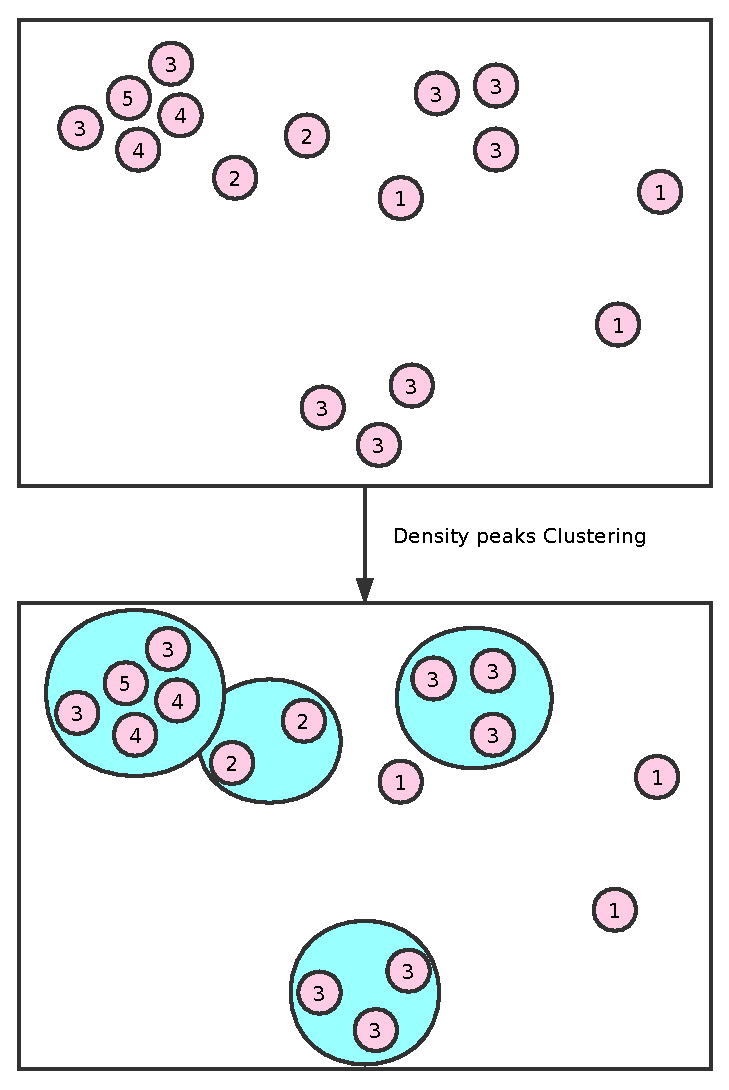
\includegraphics[width=0.7\linewidth]{density_peaks}
\caption{Illustration of DPC. The values in the pink circles indicate the number of neighbors and itself. }
\label{fig:density_peaks}
\end{figure}

\section{Probability Mixture Model}
We suppose that data $x$ is sampled from one of some probability distributions. 
Let $z$ denotes the random variable for the probability distribution, $\theta$ denotes the parameters for this probability model.
We first select a probability distribution in the probability $p\left( {z;\theta } \right)$. Then we sample $x$ from the probability distribution $p\left( {x|z;\theta } \right)$. 
Then we have the Eq.~\ref{equ:pmmBase}. 

\begin{equation}
\label{equ:pmmBase}
p\left( {x;\theta } \right) = \sum\limits_z {p\left( {x|z;\theta } \right)p\left( {z;\theta } \right)}
\end{equation}
 
The optimization object function can be formalized by Eq.~\ref{equ:pmmObjectFunction}.

\begin{equation}
\label{equ:pmmObjectFunction}
J = \frac{1}{n}\log \sum\limits_{i = 0}^{n - 1} {\sum\limits_z {p\left( {{x^{*i}}|z;\theta } \right)p\left( {z;\theta } \right)} }
\end{equation}

If we directly calculate the solution of the parameter $\theta_{k}$ ($\theta_k$ denotes the parameter for $kth$ distribution) as Eq. shown, we will find solution of $\theta_k$ is a blend of other parameters for other distributions .

\begin{equation}
\label{equ:pmm_unable_solve_parameter_directly}
\begin{aligned}
\frac{{\partial \frac{1}{n}\log \sum\limits_{i = 0}^{n - 1} {p\left( {{x^{*i}};\theta } \right)} }}{{\partial {\theta _k}}} &= \frac{1}{n}\sum\limits_{i = 0}^{n - 1} {\frac{1}{{p\left( {{x^{*i}};\theta } \right)}}} \frac{{\partial p\left( {{x^{*i}};\theta } \right)}}{{\partial {\theta _k}}}\\
 &= \frac{1}{n}\sum\limits_{i = 0}^{n - 1} {\frac{1}{{p\left( {{x^{*i}};\theta } \right)}}} \frac{{\partial \sum\limits_z {p\left( {{x^{*i}}|z;\theta } \right)p\left( {z;\theta } \right)} }}{{\partial {\theta _k}}}\\
 &= \frac{1}{n}\sum\limits_{i = 0}^{n - 1} {\frac{1}{{p\left( {{x^{*i}};\theta } \right)}}} \frac{{\partial \sum\limits_z {p\left( {{x^{*i}}|z;{\theta _z}} \right)p\left( {z;{\theta _z}} \right)} }}{{\partial {\theta _k}}}\\
 &= \frac{1}{n}\sum\limits_{i = 0}^{n - 1} {\frac{1}{{p\left( {{x^{*i}};\theta } \right)}}} \frac{{\partial \left( {p\left( {{x^{*i}}|z = k;{\theta _k}} \right)p\left( {z = k;{\theta _k}} \right)} \right)}}{{\partial {\theta _k}}}\\
 &= \frac{1}{n}\sum\limits_{i = 0}^{n - 1} {\frac{{p\left( {z = k|{x^{*i}},\theta } \right)}}{{p\left( {{x^{*i}}|z = k,{\theta _k}} \right)p\left( {z = k;{\theta _k}} \right)}}} \frac{{\partial \left( {p\left( {{x^{*i}}|z = k;{\theta _k}} \right)p\left( {z = k;{\theta _k}} \right)} \right)}}{{\partial {\theta _k}}}\\
 &= \frac{1}{n}\sum\limits_{i = 0}^{n - 1} {\frac{{p\left( {z = k|{x^{*i}},\theta } \right)}}{{p\left( {{x^{*i}}|z = k,{\theta _k}} \right)p\left( {z = k;{\theta _k}} \right)}}} \frac{{\partial \left( {p\left( {{x^{*i}}|z = k;{\theta _k}} \right)p\left( {z = k;{\theta _k}} \right)} \right)}}{{\partial {\theta _k}}}\\
 &= \frac{1}{n}\sum\limits_{i = 0}^{n - 1} {p\left( {z = k|{x^{*i}},\theta } \right)} \frac{{\partial \log \left( {p\left( {{x^{*i}}|z = k;{\theta _k}} \right)p\left( {z = k;{\theta _k}} \right)} \right)}}{{\partial {\theta _k}}}\\
 \Rightarrow {\theta _k} &= f\left( {{\theta _0},{\theta _1},{\theta _2},...} \right)
\end{aligned}
\end{equation}

Consider $z$ as hidden variable, we can apply the EM algorithm to solve the parameter estimation as discussed in Sec.\ref{sec:em}.
The solution process can be described by Fig.\ref{fig:pmmAlgorithm}.

\begin{figure}
\caption{Framework of EM algorithm for probability mixture model.}
\label{fig:pmmAlgorithm}
\begin{algorithmic}
\STATE Select the reasonable initial parameters $\theta ^{*0}$.
\LOOP 
\STATE E-step: Computer $p\left( {{z}|{x^{*i}};\theta ^{*j} } \right)$ for every data.
\STATE M-step: Computer $\theta ^{i + 1}$ by maximizing $\frac{1}{n}\sum\limits_{i = 0}^{n - 1} {\sum\limits_z {p\left( {z|{x^{*i}}} ; \theta^{*j}\right)\log p\left( {{x^{*i}},z}; \theta \right)} } $.
\IF {Stop converge or reach the maximum iterative times}
\STATE Break loop
\ENDIF
\ENDLOOP
\end{algorithmic}
\end{figure}

$p\left( {{x^{*i}}|z;\theta } \right)$ can be any type of probability distribution even the mixture probability distribution. We now discuss the most common probability distribution: Gaussian distribution.

\subsection{Gaussian Mixture Model}
Let $\alpha$ denotes the vector for probability of selection of Gaussian distributions, $\alpha_{z}$ denotes the probability for selecting $zth$ Gaussian distribution. $u$ and $\Sigma$ denote the vector for average value and variance for Gaussian distributions, $u_{z}$ and $\Sigma_{z}$ denote the average value and variance of $zth$ Gaussian distribution respectively. $\alpha^{*j}$, $u^{*j}$ and $\Sigma^{*j}$ denote the $jth$ update parameter value respectively. $d$ denotes the dimension of data. $\varepsilon_{iz}$ denotes the probability $p\left( {z|{x^{*i}};{\theta ^{*j}}} \right)$. We have Eq.~\ref{equ:pmmGMMEpsilon}.

\begin{equation}
\label{equ:pmmGMMEpsilon}
\begin{aligned}
{\varepsilon _{iz}} &= p\left( {z|{x^{*i}};{\theta ^{*j}}} \right)\\
 &= \frac{{p\left( {{x^{*i}}|z;{\theta ^{*j}}} \right)p\left( {z;{\theta ^{*j}}} \right)}}{{p\left( {{x^{*i}};{\theta ^{*j}}} \right)}}\\
 &= \frac{{p\left( {{x^{*i}}|z;{\theta ^{*j}}} \right)p\left( {z;{\theta ^{*j}}} \right)}}{{\sum\limits_{\tilde{z}} {p\left( {{x^{*i}}|\tilde{z};{\theta ^{*j}}} \right)p\left( {\tilde{z};{\theta ^{*j}}} \right)} }}\\
 &= \frac{{N\left( {{x^{*i}};{u_z}^{*j},{\Sigma _z}^{*j}} \right){\alpha _z}^{*j}}}{{\sum\limits_{\tilde{z}} {N\left( {{x^{*i}};{u_{\tilde{z}}}^{*j},{\Sigma _{\tilde{z}}}^{*j}} \right){\alpha _{\tilde{z}}}^{*j}} }}
\end{aligned}
\end{equation}

Then the maximizing object function in EM algorithm can be formalized by Eq.~\ref{equ:pmmGMMMaximizingObject}.

\begin{equation}
\label{equ:pmmGMMMaximizingObject}
\begin{aligned}
&emJ = \frac{1}{n}\sum\limits_{i = 0}^{n - 1} {\sum\limits_{z = 0}^{d - 1} {p\left( {z|{x^{*i}};{\theta ^{*j}}} \right)\log p\left( {{x^{*i}},z;\theta } \right)} } \\
 &\quad= \frac{1}{n}\sum\limits_{i = 0}^{n - 1} {\sum\limits_{z = 0}^{d - 1} {{\varepsilon _{iz}}\log p\left( {{x^{*i}},z;\theta } \right)} } \\
 &\quad= \frac{1}{n}\sum\limits_{i = 0}^{n - 1} {\sum\limits_{z = 0}^{d - 1} {{\varepsilon _{iz}}\log p\left( {{x^{*i}}|z;\theta } \right)p\left( {z|\theta } \right)} } \\
 &\quad= \frac{1}{n}\sum\limits_{i = 0}^{n - 1} {\sum\limits_{z = 0}^{d - 1} {{\varepsilon _{iz}}\log {\alpha _z}{{\left( {2\pi } \right)}^{ - \frac{d}{2}}}|\Sigma_{z} {|^{^{ - \frac{1}{2}}}}\exp \left\{ { - \frac{1}{2}\left( {{x^{*i}} - {u_z}} \right){\Sigma_{z} ^{ - 1}}{{\left( {{x^{*i}} - {u_z}} \right)}^t}} \right\}} } \\
 =& \frac{1}{n}\sum\limits_{i = 0}^{n - 1} {\sum\limits_{z = 0}^{d - 1} {{\varepsilon _{iz}}
 \left( {\log {\alpha _z} - \frac{d}{2}\log 2\pi  - \frac{1}{2}\log |\Sigma_{z} | - \frac{1}{2}\left( {{x^{*i}} - {u_z}} \right){\Sigma_{z} ^{ - 1}}{{\left( {{x^{*i}} - {u_z}} \right)}^t}} \right)}}\\
&s.t.\ \sum\limits_{z = 0}^{d - 1} {{\alpha _z}}  = 1
\end{aligned}
\end{equation}

$emJ$ has upper bound, we can calculate the derivation of $emJ$ about $\alpha$, $u$ and $\Sigma$ to find the best optimization solution for maximizing $emJ$. We first solve $\alpha$ by Eq.~\ref{equ:pmmGMMAlpha}.

\begin{equation}
\label{equ:pmmGMMAlpha}
\begin{aligned}
&L\left( {\theta ;\lambda } \right) = emJ + \lambda \left( {\sum\limits_{z = 0}^{d - 1} {{\alpha _z}}  - 1} \right)\\
\Rightarrow&\left\{ {\begin{array}{*{20}{c}}
{\frac{{\partial L\left( {\theta ;\lambda } \right)}}{{\partial {\alpha _z}}} = \frac{1}{n}\sum\limits_{i = 0}^{n - 1} {\frac{{{\varepsilon _{iz}}}}{{{\alpha _z}}}}  + \lambda  = 0}\\
{\frac{{\partial L\left( {\theta ;\lambda } \right)}}{{\partial \lambda }} = \sum\limits_{z = 0}^{d - 1} {{\alpha _z}}  - 1 = 0}
\end{array}} \right.\\
 \Rightarrow& \sum\limits_{i = 0}^{n - 1} {\frac{{{\beta _{iz}}}}{{{\alpha _z}}}}  + n\lambda  = 0\\
 \Rightarrow& \sum\limits_{i = 0}^{n - 1} {{\varepsilon _{iz}}}  =  - {\alpha _z}n\lambda \\
 \Rightarrow& {\alpha _z} =  - \frac{{\sum\limits_{i = 0}^{n - 1} {{\varepsilon _{iz}}} }}{{n\lambda }}\\
 \Rightarrow& \sum\limits_{z = 0}^{d - 1} {{\alpha _z}}  =  - \sum\limits_{z = 0}^{d - 1} {\frac{{\sum\limits_{i = 0}^{n - 1} {{\varepsilon _{iz}}} }}{{n\lambda }}} \\
 \Rightarrow& \sum\limits_{z = 0}^{d - 1} {{\alpha _z}}  =  - \frac{1}{{n\lambda }}\sum\limits_{z = 0}^{d - 1} {\sum\limits_{i = 0}^{n - 1} {{\varepsilon _{iz}}} }  =  - \frac{n}{{n\lambda }} = 1\\
 \Rightarrow& \lambda  =  - 1\\
 \Rightarrow& {\alpha _z} = \frac{{\sum\limits_{i = 0}^{n - 1} {{\varepsilon _{iz}}} }}{n}
\end{aligned}
\end{equation}

Then we solve $u$ and $\Sigma$ by Eq.~\ref{equ:pmmGMMu} and Eq.~\ref{equ:pmmGMMSigma} respectively.

\begin{equation}
\label{equ:pmmGMMu}
\begin{aligned}
&\frac{{\partial emJ}}{{\partial {u_z}}} = \frac{{\partial emJ}}{{\partial \left( {{x^{*i}} - {u_z}} \right)}}\frac{{\partial \left( {{x^{*i}} - {u_z}} \right)}}{{\partial {u_z}}}\\
 &\quad\quad= \frac{1}{n}\sum\limits_{i = 0}^{n - 1} { - {\varepsilon _{iz}}\frac{1}{2}2\left( {{x^{*i}} - {u_z}} \right){\Sigma ^{ - 1}}} \left( { - 1} \right)\\
 &\quad\quad= \frac{1}{n}\sum\limits_{i = 0}^{n - 1} {{\varepsilon _{iz}}\left( {{x^{*i}} - {u_z}} \right)} {\Sigma ^{ - 1}} = 0\\
 \Rightarrow& \sum\limits_{i = 0}^{n - 1} {{\varepsilon _{iz}}\left( {{x^{*i}} - {u_z}} \right)}  = 0\\
 \Rightarrow& \sum\limits_{i = 0}^{n - 1} {{\varepsilon _{iz}}{x^{*i}}}  = {u_z}\sum\limits_{i = 0}^{n - 1} {{\varepsilon _{iz}}}\\
 \Rightarrow& {u_z} = \frac{{\sum\limits_{i = 0}^{n - 1} {{\varepsilon _{iz}}{x^{*i}}} }}{{\sum\limits_{i = 0}^{n - 1} {{\varepsilon _{iz}}} }}
\end{aligned}
\end{equation}

\begin{equation}
\label{equ:pmmGMMSigma}
\begin{aligned}
&\frac{{\partial emJ}}{{\partial {\Sigma_{z} ^{ - 1}}}} = \frac{{\partial \frac{1}{n}\sum\limits_{i = 0}^{n - 1} {\sum\limits_{z = 0}^{d - 1} {{\varepsilon _{iz}}\left( { - \frac{1}{2}\log |\Sigma_{z} | - \frac{1}{2}\left( {{x^{*i}} - {u_z}} \right){\Sigma_{z} ^{ - 1}}{{\left( {{x^{*i}} - {u_z}} \right)}^t}} \right)} } }}{{\partial {\Sigma ^{ - 1}}}}\\
&\quad\quad = \frac{{\partial \frac{1}{n}\sum\limits_{i = 0}^{n - 1} {\sum\limits_{z = 0}^{d - 1} {{\varepsilon _{iz}}\left( {\frac{1}{2}\log |{\Sigma_{z} ^{ - 1}}| - \frac{1}{2}\left( {{x^{*i}} - {u_z}} \right){\Sigma_{z} ^{ - 1}}{{\left( {{x^{*i}} - {u_z}} \right)}^t}} \right)} } }}{{\partial {\Sigma_{z} ^{ - 1}}}}\\
&\quad\quad = \frac{1}{n}\sum\limits_{i = 0}^{n - 1} {{\varepsilon _{iz}}\left( {\frac{1}{{2|{\Sigma_{z} ^{ - 1}}|}}|{\Sigma_{z} ^{ - 1}}|{{\left( {{\Sigma_{z} ^{ - 1}}} \right)}^{ - 1}} - \frac{1}{2}{{\left( {{x^{*i}} - {u_z}} \right)}^t}\left( {{x^{*i}} - {u_z}} \right)} \right)} \\
&\quad\quad = \frac{1}{{2n}}\sum\limits_{i = 0}^{n - 1} {{\varepsilon _{iz}}\left( {\Sigma_{z}  - {{\left( {{x^{*i}} - {u_z}} \right)}^t}\left( {{x^{*i}} - {u_z}} \right)} \right)}  = 0\\
 \Rightarrow& \sum\limits_{i = 0}^{n - 1} {{\varepsilon _{iz}}\Sigma_{z}  - {\varepsilon _{iz}}{{\left( {{x^{*i}} - {u_z}} \right)}^t}\left( {{x^{*i}} - {u_z}} \right)}  = 0\\
 \Rightarrow& \Sigma_{z} \sum\limits_{i = 0}^{n - 1} {{\varepsilon _{iz}}}  - \sum\limits_{i = 0}^{n - 1} {{\varepsilon _{iz}}{{\left( {{x^{*i}} - {u_z}} \right)}^t}\left( {{x^{*i}} - {u_z}} \right)}  = 0\\
 \Rightarrow& \Sigma_{z}  = \frac{{\sum\limits_{i = 0}^{n - 1} {{\varepsilon _{iz}}{{\left( {{x^{*i}} - {u_z}} \right)}^t}\left( {{x^{*i}} - {u_z}} \right)} }}{{\sum\limits_{i = 0}^{n - 1} {{\varepsilon _{iz}}} }}
\end{aligned}
\end{equation}

\subsection{K-means}
We assume the value of $p\left( {z|{x^{*i}};{\theta ^{*j}}} \right)$ can only be $0$ or $1$, that is, all distributions are dispersive distinctly (their center are far away from each other and their variances are very small). 
If a sample $x^{*i}$ does not belongs to a distribution ($x^{*i}$ is far away from $u_z$, so $N\left(x^{*i}; u_z, \Sigma_z\right)$ will be very small), then $p\left( {z|{x^{*i}};{\theta ^{*j}}} \right) = 0$, otherwise the probability will be $1$.
Under such assumption, the result GMM turns to K-means cluster result.
$\alpha _z$, $u_z$ and $\Sigma_{z}$ are the number, center and variance of samples belong to distribution $z$.
The only initial value are the initial center $u$ of all distributions. For the initial $\Sigma$, we assume them to be very small so that $p\left( {z|{x^{*i}};{\theta ^{*j}}} \right)$ will be $0$ when a sample $x^{*i}$ is far away from the center of $u_z$.
For $\alpha$, it can be any value.

\subsection{Gaussian Mixture-Mixture Model}
In previous section, we discuss the derivation when probability distribution is Gaussian distribution. Now we talk about the probability is distribution Gaussian mixture distribution (we call it GMMM). In some cluster problems, the data of one category can not be described well by one pure probability distribution thus we need to adopt the mixture probability distribution (most times we use Gaussian mixture distribution). We redefine the $p\left(x; \theta\right)$ as shown in Eq.~\ref{equ:pmmMixtureMixtureProbability}.

\begin{equation}
\label{equ:pmmMixtureMixtureProbability}
p\left( {x;\theta } \right) = \sum\limits_{z = 0}^{d - 1} {p\left( {z;\theta } \right)p\left( {x|z;\theta } \right)}  = \sum\limits_{z = 0}^{d - 1} {p\left( {z;\theta } \right)\sum\limits_{{r_z} = 0}^{{c_z} - 1} {p\left( {{r_z};\theta } \right)p\left( {x|{r_z};\theta } \right)} } 
\end{equation}
Where $z$ is the random variable for selecting Gaussian mixture distribution (the count of type is $d$). $r_{z}$ is the random variable for selecting Gaussian distribution in Gaussian mixture distribution $z$ (the count of type is $c_{r_{z}}$). That is to say, in order to sample one data $x$, we first select a Gaussian mixture model $p\left( {x|z;\theta } \right)$ in the probability of $p\left( {z;\theta } \right) = \alpha_{z}$, then select a Gaussian distribution ${p\left( {x|{r_z};\theta } \right)}$ in the probability of $p\left( {{r_z};\theta } \right) = \beta_{r_z}$) and sample data from it. 

In this type, the optimization object function can be simplified by Eq.~\ref{equ:pmmMixtureMixtureOOF}.

\begin{equation}
\label{equ:pmmMixtureMixtureOOF}
\begin{aligned}
J &= \frac{1}{n}\sum\limits_{i = 0}^{n - 1} {\log \sum\limits_{z = 0}^{d - 1} {p\left( {{x^{*i}},z;\theta } \right)} } \\
 &= \frac{1}{n}\sum\limits_{i = 0}^{n - 1} {\sum\limits_{z = 0}^{d - 1} {p\left( {z|{x^{*i}};\theta } \right)\log \frac{{p\left( {{x^{*i}},z;\theta } \right)}}{{p\left( {z|{x^{*i}};\theta } \right)}}} } \\
 &= \frac{1}{n}\sum\limits_{i = 0}^{n - 1} {\sum\limits_{z = 0}^{d - 1} {p\left( {z|{x^{*i}};\theta } \right)\left( {\log p\left( {{x^{*i}},z;\theta } \right) - \log p\left( {z|{x^{*i}};\theta } \right)} \right)} } \\
 &= \frac{1}{n}\sum\limits_{i = 0}^{n - 1} {\sum\limits_{z = 0}^{d - 1} {p\left( {z|{x^{*i}};\theta } \right)\left( {\log p\left( z \right)\sum\limits_{{r_z} = 0}^{{c_z} - 1} {p\left( {{x^{*i}},{r_z};\theta } \right)}  - \log p\left( {z|{x^{*i}};\theta } \right)} \right)} } \\
 &= \frac{1}{n}\sum\limits_{i = 0}^{n - 1} {\sum\limits_{z = 0}^{d - 1} {p\left( {z|{x^{*i}};\theta } \right)\left( {\log p\left( {z;\theta } \right) + \log \sum\limits_{{r_z} = 0}^{{c_z} - 1} {p\left( {{x^{*i}},{r_z};\theta } \right)}  - \log p\left( {z|{x^{*i}};\theta } \right)} \right)} } \\
 & = \frac{1}{n}\sum\limits_{i = 0}^{n - 1} {\sum\limits_{z = 0}^{d - 1} {p\left( {z|{x^{*i}};\theta } \right)\left( \begin{array}{l}
\log p\left( {z;\theta } \right) + \sum\limits_{{r_z} = 0}^{{c_z} - 1} {p\left( {{r_z}|{x^{*i}};\theta } \right)\log \frac{{p\left( {{x^{*i}},{r_z};\theta } \right)}}{{p\left( {{r_z}|{x^{*i}};\theta } \right)}}} \\
 - \log p\left( {z|{x^{*i}};\theta } \right)
\end{array} \right)} } 
\end{aligned}
\end{equation}

The EM algorithm here can be described as Fig.\ref{fig:pmmMixtureMixtureAlgorithm}. The computation equations are shown from Eq.~\ref{equ:pmmMixtureMixtureEpsilon} to Eq.~\ref{equ:pmmMixtureMixtureDerivationResult}. We leave out the derivation processing due to it is very similar to the processing in GMM.

\begin{figure}
\caption{Framework of EM algorithm for probability mixture model.}
\label{fig:pmmMixtureMixtureAlgorithm}
\begin{algorithmic}
\STATE Select the reasonable initial parameters $\theta ^{*0}$.
\LOOP 
\STATE E-step: Computer $p\left( {{z}|{x^{*i}};\theta ^{*j} } \right)$ and $p\left( {{r_z}|{x^{*i}};{\theta ^{*j}}} \right)$ for every data.
\STATE M-step: Computer $\theta ^{i + 1}$ by maximizing 
\begin{displaymath}
\frac{1}{n}\sum\limits_{i = 0}^{n - 1} {\sum\limits_{z = 0}^{d - 1} {p\left( {z|{x^{*i}};{\theta ^{*j}}} \right)\left( {\log p\left( {z;\theta } \right) + \sum\limits_{{r_z} = 0}^{{c_z} - 1} {p\left( {{r_z}|{x^{*i}};{\theta ^{*j}}} \right)\log p\left( {{x^{*i}},{r_z};\theta } \right)} } \right)} }
\end{displaymath}
\IF {Stop converge or reach the maximum iterative times}
\STATE Break loop
\ENDIF
\ENDLOOP
\end{algorithmic}
\end{figure}

\begin{equation}
\label{equ:pmmMixtureMixtureEpsilon}
\begin{aligned}
{\varepsilon _{iz}} &= p\left( {z|{x^{*i}};{\theta ^{*j}}} \right) = \frac{{p\left( {z,{x^{*i}};{\theta ^{*j}}} \right)}}{{\sum\limits_{\tilde z = 0}^{d - 1} {p\left( {\tilde z,{x^{*i}};{\theta ^{*j}}} \right)} }}\\
 &= \frac{{p\left( {z;{\theta ^{*j}}} \right)p\left( {{x^{*i}}|z;{\theta ^{*j}}} \right)}}{{\sum\limits_{\tilde z = 0}^{d - 1} {p\left( {\tilde z,{x^{*i}};{\theta ^{*j}}} \right)} }}\\
 &= \frac{{p\left( {z;{\theta ^{*j}}} \right)\sum\limits_{{r_z} = 0}^{{c_z} - 1} {p\left( {{x^{*i}},{r_z};{\theta ^{*j}}} \right)} }}{{\sum\limits_{\tilde z = 0}^{d - 1} {p\left( {\tilde z,{x^{*i}};{\theta ^{*j}}} \right)} }}\\
 &= \frac{{p\left( {z;{\theta ^{*j}}} \right)\sum\limits_{{r_z} = 0}^{{c_z} - 1} {p\left( {{x^{*i}}|{r_z};{\theta ^{*j}}} \right)p\left( {{r_z};{\theta ^{*j}}} \right)} }}{{\sum\limits_{\tilde z = 0}^{d - 1} {p\left( {\tilde z;{\theta ^{*j}}} \right)\sum\limits_{{r_{\tilde z}} = 0}^{{c_{\tilde z}} - 1} {p\left( {{x^{*i}}|{r_{\tilde z}};{\theta ^{*j}}} \right)p\left( {{r_{\tilde z}};{\theta ^{*j}}} \right)} } }}\\
 &= \frac{{{\alpha _z}^{*j}\sum\limits_{{r_z} = 0}^{{c_z} - 1} {N\left( {{x^{*i}};{u_{{r_z}}}^{*j};{\Sigma _{{r_z}}}^{*j}} \right){\beta _{{r_z}}}^{*j}} }}{{\sum\limits_{\tilde z = 0}^{d - 1} {{\alpha _{\tilde z}}^{*j}\sum\limits_{{r_{\tilde z}} = 0}^{{c_{\tilde z}} - 1} {N\left( {{x^{*i}};{u_{{r_{\tilde z}}}}^{*j};{\Sigma _{{r_{\tilde z}}}}^{*j}} \right){\beta _{{r_{\tilde z}}}}^{*j}} } }}
\end{aligned}
\end{equation}

\begin{equation}
\label{equ:pmmMixtureMixturePhi}
\begin{aligned}
{\phi _{i{r_z}}} &= p\left( {{r_z}|{x^{*i}};{\theta ^{*j}}} \right)\\
 &= \frac{{p\left( {{r_z};{\theta ^{*j}}} \right)p\left( {{x^{*i}}|{r_z};{\theta ^{*j}}} \right)}}{{\sum\limits_{{{\tilde r}_z} = 0}^{{c_z} - 1} {p\left( {{{\tilde r}_z};{\theta ^{*j}}} \right)p\left( {{x^{*i}}|{{\tilde r}_z};{\theta ^{*j}}} \right)} }}\\
 &= \frac{{{\beta _{{r_z}}}^{*j}N\left( {{x^{*i}};{u_{{r_z}}}^{*j};{\Sigma _{{r_z}}}^{*j}} \right)}}{{\sum\limits_{{{\tilde r}_z} = 0}^{{c_z} - 1} {{\beta _{{{\tilde r}_z}}}^{*j}N\left( {{x^{*i}};{u_{{{\tilde r}_z}}}^{*j};{\Sigma _{{{\tilde r}_z}}}^{*j}} \right)} }}
\end{aligned}
\end{equation}

\begin{equation}
\label{equ:pmmMixtureMixtureEMJ}
\begin{aligned}
&emJ = \frac{1}{n}\sum\limits_{i = 0}^{n - 1} {\sum\limits_{z = 0}^{d - 1} {{\varepsilon _{iz}}\left( {\log p\left( {z;\theta } \right) + \sum\limits_{{r_z} = 0}^{{c_z} - 1} {{\phi _{i{r_z}}}\log p\left( {{x^{*i}},{r_z};\theta } \right)} } \right)} } \\
 &\quad= \frac{1}{n}\sum\limits_{i = 0}^{n - 1} {\sum\limits_{z = 0}^{d - 1} {{\varepsilon _{iz}}\left( {\log {\alpha _z} + \sum\limits_{{r_z} = 0}^{{c_z} - 1} {{\phi _{i{r_z}}}\log p\left( {{r_z};\theta } \right)p\left( {{x^{*i}}|{r_z};\theta } \right)} } \right)} } \\
 &\quad= \frac{1}{n}\sum\limits_{i = 0}^{n - 1} {\sum\limits_{z = 0}^{d - 1} {{\varepsilon _{iz}}\left( {\log {\alpha _z} + \sum\limits_{{r_z} = 0}^{{c_z} - 1} {{\phi _{i{r_z}}}\log {\beta _{{r_z}}}p\left( {{x^{*i}}|{r_z};\theta } \right)} } \right)} } \\
 &\ = \frac{1}{n}\sum\limits_{i = 0}^{n - 1} {\sum\limits_{z = 0}^{d - 1} {{\varepsilon _{iz}}\left( \begin{array}{l}
\log {\alpha _z} + \\
\sum\limits_{{r_z} = 0}^{{c_z} - 1} {{\phi _{i{r_z}}}\log {\beta _{{r_z}}}\left( \begin{array}{l}
{\left( {2\pi } \right)^{ - \frac{d}{2}}}|{\Sigma _{{r_z}}}{|^{ - \frac{1}{2}}}\exp \\
\left\{ { - \frac{1}{2}\left( {{x^{*i}} - {u_{{r_z}}}} \right){\Sigma _{{r_z}}}^{ - 1}{{\left( {{x^{*i}} - {u_{{r_z}}}} \right)}^t}} \right\}
\end{array} \right)} 
\end{array} \right)} } \\
 &\quad= \frac{1}{n}\sum\limits_{i = 0}^{n - 1} {\sum\limits_{z = 0}^{d - 1} {{\varepsilon _{iz}}\left( \begin{array}{l}
\log {\alpha _z} + \\
\sum\limits_{{r_z} = 0}^{{c_z} - 1} {{\phi _{i{r_z}}}\left( \begin{array}{l}
\log {\beta _{{r_z}}} - \frac{d}{2}\log 2\pi  - \frac{1}{2}\log |{\Sigma _{{r_z}}}|\\
 - \frac{1}{2}\left( {{x^{*i}} - {u_{{r_z}}}} \right){\Sigma _{{r_z}}}^{ - 1}{\left( {{x^{*i}} - {u_{{r_z}}}} \right)^t}
\end{array} \right)} 
\end{array} \right)} } \\
&s.t.\ \sum\limits_{z = 0}^{d - 1} {{\alpha _z}}  = 1,\ \sum\limits_{{r_z} = 0}^{{c_z} - 1} {{\beta _{r_z}}}  = 1
\end{aligned}
\end{equation}

\begin{equation}
\label{equ:pmmMixtureMixtureDerivationResult}
\begin{aligned}
{\alpha _z} &= \frac{{\sum\limits_{i = 0}^{n - 1} {{\varepsilon _{iz}}} }}{n}\\
{\beta _{{r_z}}} &= \frac{{\sum\limits_{i = 0}^{n - 1} {{\varepsilon _{iz}}{\phi _{i{r_z}}}} }}{n}\\
{u_{{r_z}}} &= \frac{{\sum\limits_{i = 0}^{n - 1} {{\varepsilon _{iz}}{\phi _{i{r_z}}}{x^{*i}}} }}{n}\\
{\Sigma _{{r_z}}} &= \frac{{\sum\limits_{i = 0}^{n - 1} {{\varepsilon _{iz}}{\phi _{i{r_z}}}{{\left( {{x^{*i}} - {u_{r_z}}} \right)}^t}\left( {{x^{*i}} - {u_{r_z}}} \right)} }}{{\sum\limits_{i = 0}^{n - 1} {{\varepsilon _{iz}}{\phi _{i{r_z}}}} }}
\end{aligned}
\end{equation}

\label{sec:gmm}
\chapter{Representation Models}
\section{DBN}
Inspired by the architectural depth of the brain\footnote{This section refers to the paper of \cite{DeepAI_Bengio_2009}.}, neural network researchers had wanted for decades to train deep multi-layer neural networks, but no successful attempts were reported before 2006 : researchers reported positive experimental results with typically two or three levels (i.e., one or two hidden layers), but training deeper networks consistently yielded poorer results. Something that can be considered a breakthrough happened in 2006 : Hinton et al. at University of Toronto introduced Deep Belief Network (DBN), with a learning algorithm that greedily trains one layer at a time, exploiting an unsupervised learning algorithm for each layer, a Restricted Boltzmann Machine (RBM)\cite{DeepAI_Bengio_2009}.

Shortly, DBN is based on stacking multiple RBMs, which are particular energy-based models. DBN can learns effective features that can use to other classifiers or initializes the parameters of BP neural networks.

In this section, we first introduce the theories of energy based models. Then we discuss the theories of BM, RBM and DBN.

\subsection{Energy Based Models}
Energy based models associate a scalar energy to each configuration of the interesting variables. Learning corresponds to modifying that energy function so that its shape has desirable properties. For example, we would like desirable configurations to have low energy (state with low energy often means stable state in physics, i.e., the water with very high temperature is boiling while the ice is concretionary). Energy based probabilistic models may define a marginal probability function (PMF for discrete variable and PDF for continuous variable) through an energy function as Eq.~\ref{equ:dbnPDFByEnergy}.

\begin{equation}
\label{equ:dbnPDFByEnergy}
p\left( x \right) = \frac{{{e^{ - energy\left( x \right)}}}}{{\sum\limits_x {energy\left( x \right)} }} = \frac{{{e^{ - energy\left( x \right)}}}}{z}
\end{equation}
Where $z$ is called the partition function by analogy with physical systems. $z$ is the sum running over the input space, or an appropriate integral when $x$ is continuous. We select exponential function to make sure the value be positive and property of decreasing value when the energy increases. 

In the product of experts formulation, the energy function is a sum of terms, each one associated with an "expert" $f_i$ as Eq.~\ref{equ:dbnExpertEnergy}.

\begin{equation}
\label{equ:dbnExpertEnergy}
energy\left( x \right) = \sum\limits_i {{f_i}\left( x \right)}
\end{equation}

In many cases of interest, $x$ has many component variables $x_i$, and we want to introduce some non-observed variables to increase the expressive power of the model. So we consider an visible part $v$ (other representation of $x$) and a hidden part $h$. We define the joint probability function as Eq.~\ref{equ:dbnJointPFOfVisibleAndHidden}

\begin{equation}
\label{equ:dbnJointPFOfVisibleAndHidden}
p\left( {v,h} \right) = \frac{{{e^{ - energy\left( {v,h} \right)}}}}{{\sum\limits_{\tilde v} {\sum\limits_{\tilde h} {energy\left( {\tilde v,\tilde h} \right)} } }} = \frac{{{e^{ - energy\left( {v,h} \right)}}}}{z}
\end{equation}
and the marginal probability function of $v$ can be described by Eq.~\ref{equ:dbnMarginalPFOfVisible}. Note that all sums can be replaced by integral if $h$ is continuous, and the same principles apply.

\begin{equation}
\label{equ:dbnMarginalPFOfVisible}
\begin{aligned}
p\left( v \right) &= \sum\limits_h {p\left( {v,h} \right)} \\
 &= \frac{{\sum\limits_h {{e^{ - energy\left( {v,h} \right)}}} }}{z}\\
\end{aligned}
\end{equation}

In such cases, to map this formula to one similar to Eq.~\ref{equ:dbnPDFByEnergy}, we introduce the notation (inspired from physics) of \emph{free energy}, defined as Eq.~\ref{equ:dbnFreeEnergy}.

\begin{equation}
\label{equ:dbnFreeEnergy}
\begin{aligned}
&p\left( v \right) = \frac{{{e^{ - freeEnergy\left( v \right)}}}}{z} = \frac{{\sum\limits_h {energy\left( {v,h} \right)} }}{z}\\
 \Rightarrow& \left\{ {\begin{array}{*{20}{c}}
{freeEnergy\left( v \right) =  - \log \sum\limits_h {energy\left( {v,h} \right)} }\\
{z = \sum\limits_v {{e^{ - freeEnergy\left( v \right)}}}  = \sum\limits_v {\sum\limits_h {energy\left( {v,h} \right)} } }
\end{array}} \right.
\end{aligned}
\end{equation}

So the free energy is just a marginalization of energies in the log domain. The data log-likelihood gradient then has a particularly interesting form. Let us introduce $\theta$ to represent parameters of the model. Starting from Eq.~\ref{equ:dbnFreeEnergy}, we obtain Eq.~\ref{equ:dbnFreeEnergyDerivative}.

\begin{equation}
\label{equ:dbnFreeEnergyDerivative}
\begin{aligned}
\frac{{\partial \log p\left( v \right)}}{{\partial \theta }} &=  - \frac{{\partial freeEnergy\left( v \right)}}{{\partial \theta }} + \frac{1}{z}\sum\limits_{\tilde v} {{e^{ - freeEnergy\left( {\tilde v} \right)}}\frac{{\partial freeEnergy\left( {\tilde v} \right)}}{{\partial \theta }}} \\
 &=  - \frac{{\partial freeEnergy\left( v \right)}}{{\partial \theta }} + \sum\limits_{\tilde v} {p\left( {\tilde v} \right)\frac{{\partial freeEnergy\left( {\tilde v} \right)}}{{\partial \theta }}} 
\end{aligned}
\end{equation} 

If the energy function can be written as a sum of terms associated with at most one hidden unit, as shown in Eq.~\ref{equ:dbnSepcialEnergyFunction}. This is the way that RBMs do. 

\begin{equation}
\label{equ:dbnSepcialEnergyFunction}
energy\left( {v,h} \right) =  - \beta \left( v \right) + \sum\limits_i {\gamma ^{*i}\left( {v,{h_i}} \right)}
\end{equation}
Then the free energy and probability function of the visible variable $v$ can be computed tractably (even though it involves a sum with an exponential number of terms). Specifically, we first format the $p\left(v\right)$ as Eq.~\ref{equ:dbnFreeEnergyTracable1}.

\begin{equation}
\label{equ:dbnFreeEnergyTracable1}
\begin{aligned}
p\left( v \right) &= \frac{1}{z}{e^{ - freeEnergy\left( v \right)}} = \frac{1}{z}\sum\limits_h {{e^{ - energy\left( {v,h} \right)}}} \\
 &= \frac{1}{z}\sum\limits_{{h_0}} {\sum\limits_{{h_1}} {\sum\limits_{{h_2}} {...{e^{\beta \left( v \right) - \sum\limits_i {{\gamma ^{*i}}\left( {v,{h_i}} \right)} }}} } } \\
 &= \frac{{{e^{\beta \left( v \right)}}}}{z}\sum\limits_{{h_0}} {\sum\limits_{{h_1}} {\sum\limits_{{h_2}} {...{e^{ - \sum\limits_i {{\gamma ^{*i}}\left( {v,{h_i}} \right)} }}} } } \\
 &= \frac{{{e^{\beta \left( v \right)}}}}{z}\sum\limits_{{h_0}} {\sum\limits_{{h_1}} {\sum\limits_{{h_2}} {...\prod\limits_i {{e^{^{ - {\gamma ^{*i}}\left( {v,{h_i}} \right)}}}} } } } \\
 &= \frac{{{e^{\beta \left( v \right)}}}}{z}\sum\limits_{{h_0}} {{e^{ - {\gamma ^{*0}}\left( {v,{h_0}} \right)}}} \sum\limits_{{h_1}} {{e^{ - {\gamma ^{*1}}\left( {v,{h_1}} \right)}}} \sum\limits_{{h_2}} {{e^{ - {\gamma ^{*2}}\left( {v,{h_2}} \right)}}} ...\\
 &= \frac{{{e^{\beta \left( v \right)}}}}{z}\prod\limits_i {\sum\limits_{{h_i}} {{e^{ - {\gamma ^{*i}}\left( {v,{h_i}} \right)}}} } 
\end{aligned}
\end{equation}
Then we acquire the free energy function by Eq.~\ref{equ:dbnFreeEnergyTracable2}.

\begin{equation}
\label{equ:dbnFreeEnergyTracable2}
\begin{aligned}
freeEnergy\left( v \right) &=  - \log {e^{\beta \left( v \right)}}\prod\limits_i {\sum\limits_{{h_i}} {{e^{ - {\gamma ^{*i}}\left( {v,{h_i}} \right)}}} } \\
 &=  - \log {e^{\beta \left( v \right)}} - \log \prod\limits_i {\sum\limits_{{h_i}} {{e^{ - {\gamma ^{*i}}\left( {v,{h_i}} \right)}}} } \\
 &=  - \log {e^{\beta \left( v \right)}} - \sum\limits_i {\log } \sum\limits_{{h_i}} {{e^{ - {\gamma ^{*i}}\left( {v,{h_i}} \right)}}} 
\end{aligned}
\end{equation}

As the derivation in above, the parameters estimation by applying MLE is actually simple. The derivative of free energy can be computed directly and the sum term in the latter of Eq.~\ref{equ:dbnFreeEnergyDerivative} can be computed in sample way, such as MCMC method. We will take RBM as an example to illustrate the procedure of parameters estimation in Sec.\ref{sec:dbnRBM}.

What if the energy function can not be written as the special formula? Here we have the normal way to estimate the parameters.
The data log-likelihood gradient as shown in Eq.~\ref{equ:dbnEnergyModelLogLikelihoodGradient}.

\begin{equation}
\label{equ:dbnEnergyModelLogLikelihoodGradient}
\begin{aligned}
&\frac{{\partial \log p\left( v \right)}}{{\partial \theta }} = \frac{{\partial \log \frac{{\sum\limits_h {{e^{ - energy\left( {v,h} \right)}}} }}{{\sum\limits_{\tilde v} {\sum\limits_h {{e^{ - energy\left( {\tilde v,h} \right)}}} } }}}}{{\partial \theta }}\\
 & = \frac{{\partial \log \sum\limits_h {{e^{ - energy\left( {v,h} \right)}}} }}{{\partial \theta }} - \frac{{\partial \log \sum\limits_{\tilde v} {\sum\limits_h {{e^{ - energy\left( {\tilde v,h} \right)}}} } }}{{\partial \theta }}\\
 &= \frac{1}{{\sum\limits_h {{e^{ - energy\left( {v,h} \right)}}} }}\frac{{\partial \sum\limits_h {{e^{ - energy\left( {v,h} \right)}}} }}{{\partial \theta }} - \frac{1}{{\sum\limits_{\tilde v} {\sum\limits_h {{e^{ - energy\left( {\tilde v,h} \right)}}} } }}\frac{{\partial \sum\limits_{\tilde v} {\sum\limits_h {{e^{ - energy\left( {\tilde v,h} \right)}}} } }}{{\partial \theta }}\\
 & =  - \frac{{\sum\limits_h {{e^{ - energy\left( {v,h} \right)}}\frac{{\partial energy\left( {v,h} \right)}}{{\partial \theta }}} }}{{\sum\limits_h {{e^{ - energy\left( {v,h} \right)}}} }} + \frac{{\sum\limits_{\tilde v} {\sum\limits_h {{e^{ - energy\left( {\tilde v,h} \right)}}\frac{{\partial energy\left( {\tilde v,h} \right)}}{{\partial \theta }}} } }}{z}\\
 & =  - \sum\limits_h {\frac{{\frac{{{e^{ - energy\left( {v,h} \right)}}}}{z}}}{{\sum\limits_{\tilde h} {\frac{{{e^{ - energy\left( {v,\tilde h} \right)}}}}{z}} }}\frac{{\partial energy\left( {v,h} \right)}}{{\partial \theta }}}  + \sum\limits_{\tilde v} {\sum\limits_h {\frac{{{e^{ - energy\left( {\tilde v,h} \right)}}}}{z}\frac{{\partial energy\left( {\tilde v,h} \right)}}{{\partial \theta }}} } \\
 & =  - \sum\limits_h {\frac{{p\left( {v,h} \right)}}{{p\left( v \right)}}\frac{{\partial energy\left( {v,h} \right)}}{{\partial \theta }}}  + \sum\limits_{\tilde v} {\sum\limits_h {p\left( {\tilde v,h} \right)\frac{{\partial energy\left( {\tilde v,h} \right)}}{{\partial \theta }}} } \\
 &=  - \sum\limits_h {p\left( {h|v} \right)\frac{{\partial energy\left( {v,h} \right)}}{{\partial \theta }}}  + \sum\limits_{\tilde v} {\sum\limits_h {p\left( {\tilde v,h} \right)\frac{{\partial energy\left( {\tilde v,h} \right)}}{{\partial \theta }}} } 
\end{aligned}
\end{equation}

Note that the $\frac{{\partial energy\left( {v,h} \right)}}{{\partial \theta }}$ is easy to compute. Hence if we have a procedure to sample from $P\left(h|v\right)$ and one to sample from $P\left(v,h\right)$, we can obtain an unbiased stochastic estimator of the log-likelihood gradient. We will discuss the detailed procedure in Sec.\ref{sec:dbnBM}.

\subsection{Boltzmann Machine}
\label{sec:dbnBM}
The Boltzmann machine is a particular type of energy based model with hidden variables, as shown in Fig.~\ref{fig:dbn_bm}, and RBMs are special forms of Boltzmann machine in which $P\left(h|v\right)$ and $P\left(v|h\right)$ are both tractable because they factorize. In a Boltzmann machine, the energy function is a general second-order polynomial as Eq.~\ref{equ:dbnBMEnergy}.

\begin{figure}
\centering
\includegraphics[width=0.6\linewidth]{dbn_bm}
\caption{Illustration of Boltzmann machine. Note that every node are connected to all other nodes and even itself.}
\label{fig:dbn_bm}
\end{figure}

\begin{equation}
\label{equ:dbnBMEnergy}
energy\left( {v,h} \right) =  - v{b^t} - h{c^t} - vw{h^t} - vg{v^t} - hk{h^t}
\end{equation}
Where $b_{i}$ and $c_{i}$ each associated with a single element in the vector of $v$ or $h$, and the weight $w_{ij}$, $g_{ij}$ and $k_{ij}$ each associated with a pair of units. 
Matrices $g$ and $k$ should better be symmetric. For example, if $g$ is not symmetric, the extra degree of freedom would be wasted as demonstrated in Eq.~\ref{equ:dbnBMJustifySymmetric}.

\begin{equation}
\label{equ:dbnBMJustifySymmetric}
\begin{aligned}
vg{v^t} &= \sum\limits_i {\sum\limits_j {{v_i}{g_{ij}}{v_j}} } \\
 &= \sum\limits_{i = 0}^{n - 1} {\sum\limits_{j = i + 1}^{n - 1} {{v_i}{g_{ij}}{v_j} + {v_j}{g_{ji}}{v_i}} }  + \sum\limits_i {{v_i}{g_{ii}}{v_i}} \\
 &= \sum\limits_{i = 0}^{n - 1} {\sum\limits_{j = i + 1}^{n - 1} {{v_i}\left( {{g_{ij}} + {g_{ji}}} \right){v_j}} }  + \sum\limits_i {{v_i}{g_{ii}}{v_i}} \\
let\quad {g_{ij}} &= {g_{ji}} = \frac{{{{\tilde g}_{ij}}}}{2}\\
vg{v^t} &= \sum\limits_{i = 0}^{n - 1} {\sum\limits_{j = i + 1}^{n - 1} {{v_i}{{\tilde g}_{ij}}{v_j}} }  + \sum\limits_i {{v_i}\frac{{{{\tilde g}_{ii}}}}{2}{v_i}} 
\end{aligned}
\end{equation}
Where the ${g_{ij}} + {g_{ji}}$ can be combined to a ${{\tilde g}_{ij}}$ so that $vg{v^t}$ is equivalent to $v\tilde g{v^t}$ and $\tilde{g}$ is symmetric that has lower degree of freedom. Thus we should assume the $g$ and $k$ to be symmetric.
To make Eq.~\ref{equ:dbnBMJustifySymmetric} has no duplicated terms, $g$ and $k$ should be 
upper triangular matrix whose values in bottom half are zero (the diagonal are also most times zeros).

Because of the quadratic interaction terms in $h$, the trick to analytically compute the free energy can not be applied here. We only can solve the problem from Eq.~\ref{equ:dbnEnergyModelLogLikelihoodGradient}.
Specifically, an MCMC sampling procedure can be applied in order to obtain a stochastic estimator of the gradient. We can adopt the following terminology: in the positive phase, $v$ is clamped to the observed input vector, and we sample $h$ given $v$; in the negative phase both $v$ and $h$ are sampled, ideally from the model itself. In order to achieve the highly sampling efficiency, we choose the MCMC method based on Gibbs sampling.

Let $s = \left(v, h\right)$ denote all the units in the Boltzmann machine, and $s_{-i}$ the set of values associated with all units except the $ith$ one.
The Boltzmann machine energy function Eq.~\ref{equ:dbnBMEnergy} can be rewritten by putting all the parameters in a vector $d$ and a symmetric matrix $m$ (we define the triangular matrix for $m$ is $\hat{m}$, the bottom half except diagonal of $\hat m$ is $0$), for the BM in Fig.~\ref{fig:dbn_bm_example_three_units}, we have

\begin{figure}
\centering
\includegraphics[width=0.6\linewidth]{dbn_bm_example_three_units}
\caption{Illustration of Boltzmann machine contains two visible units and one hidden unit.}
\label{fig:dbn_bm_example_three_units}
\end{figure}


\begin{displaymath}
\label{equ:dbn_bm_example_rewritten_energy_three_units}
\begin{aligned}
energy\left( s \right) &=  - {s_0}{d_0} - {s_1}{d_1} - {s_2}{d_2}\\
 &\quad\quad - {s_0}{m_{00}}{s_0} - {s_1}{m_{11}}{s_1} - {s_2}{m_{22}}{s_2}\\
 &\quad\quad - {s_0}{m_{01}}{s_1} - {s_0}{m_{02}}{s_2} - {s_1}{m_{02}}s{}_2\\
 &=  - s{d^t} - s\hat m{s^t}
\end{aligned}
\end{displaymath}
Thus we have the rewritting energy function as Eq.~\ref{equ:dbn_bm_rewritten_energy}.

\begin{equation}
\label{equ:dbn_bm_rewritten_energy}
energy\left( s \right) =  - s{d^t} - s\hat m{s^t}
\end{equation}

Let $d_{-i}$ denotes the vector $d$ without the element $d_i$, 
${{m_{\_i}}}$ denotes the $i-th$ colum vector of matrix $m$,
${{{\hat m}_{ - i}}}$ denotes the matrix $\hat m$ without the $ith$ row and colum.
Using this notation, we obtain that $p\left(s_{i}|s_{-i}\right)$ can be computed and sampled from easily in a Boltzmann machine.
For example, if $s_i \in \left\{ {0, 1} \right\}$,

\begin{displaymath}
\label{equ:dbn_bm_condition_probability}
\begin{aligned}
p\left( {{s_i} = 1|{s_{ - i}}} \right) &= \frac{{p\left( {{s_i} = 1,{s_{ - i}}} \right)}}{{p\left( {{s_i} = 1,{s_{ - i}}} \right) + p\left( {{s_i} = 0,{s_{ - i}}} \right)}}\\
 &= \frac{{\exp \left( {{d_i} + {s_{ - i}}{d_{ - i}}^t + {s_{ - i}}{{\left( {{m_{\_i}}} \right)}_{ - i}} + {s_{ - i}}{{\hat m}_{ - i}}{s_{ - i}}^t - {{\hat m}_{ii}}} \right)}}{\begin{array}{l}
\exp \left( {{d_i} + {s_{ - i}}{d_{ - i}}^t + {s_{ - i}}{{\left( {{m_{\_i}}} \right)}_{ - i}} + {s_{ - i}}{{\hat m}_{ - i}}{s_{ - i}}^t - {{\hat m}_{ii}}} \right)\\
 + \exp \left( {{s_{ - i}}{d_{ - i}}^t + {s_{ - i}}{{\hat m}_{ - i}}{s_{ - i}}^t} \right)
\end{array}}\\
 &= \frac{{\exp \left( {{d_i} + {s_{ - i}}{{\left( {{m_{\_i}}} \right)}_{ - i}} - {{\hat m}_{ii}}} \right)}}{{\exp \left( {{d_i} + {s_{ - i}}{{\left( {{m_{\_i}}} \right)}_{ - i}} - {{\hat m}_{ii}}} \right) + 1}}\\
 &= \frac{1}{{1 + {{\exp }^{ - {d_i} - {s_{ - i}}{{\left( {{m_{\_i}}} \right)}_{ - i}} - {{\hat m}_{ii}}}}}}\\
 &= sigmoid\left( { - {d_i} - {s_{ - i}}{{\left( {{m_{\_i}}} \right)}_{ - i}} - {{\hat m}_{ii}}} \right)
\end{aligned}
\end{displaymath}
which is essentially the usual equation for computing a neuron's output in terms of other neurons $s_{-i}$, in artificial neural networks when ${{{\hat m}_{ii}}}$ is zero (that is there is no self connection in Boltzmann machine).
Once get the condition probability, we can adopt the Gibbs sampling to approximate the Eq.~\ref{equ:dbnEnergyModelLogLikelihoodGradient}.

Since two MCMC chains (one for the positive phase and one for the negative phase) are needed for each example $x$, the computation of the gradient can be very expensive, and training time very long.
This is essentially why Boltzmann machine was replaced in the late 1980's by the back propagation algorithm for multi-layer neural networks as the dominant learning approach.
However, recent work has shown that short chains can sometimes be used successfully, and this is the principle of Contrastive Divergence, to train RBMs.

\subsection{Binary Restricted Boltzmann Machine}
\label{sec:dbnRBM}
The Restricted Boltzmann Machine (RBM) is the building block of a Deep Belief Network (DBN) it shares parametrization with individual layers of a DBN, and becasue efficient learning algorithms were found to train it, as shown in Fig.~\ref{fig:dbn_rbm}.
In an RBM, $g = 0$ and $k = 0$ in Eq.~\ref{equ:dbnBMEnergy}, the only interaction are between a hidden unit and a visible unit, but not between units of the same layer.
Hence the visible units are independent of each other and so are hidden units.

\begin{figure}
\centering
\includegraphics[width=0.6\linewidth]{dbn_rbm}
\caption{Illustration of Restricted Boltzmann machine.}
\label{fig:dbn_rbm}
\end{figure}

The energy function can be formalized by

\begin{displaymath}
\label{equ:dbn_rbm_energy}
energy\left( {v,h} \right) =  - v{b^t} - h{c^t} - vw{h^t}
\end{displaymath}

Let $\beta \left( v \right) = v{b^t}$, ${\gamma _i}\left( {v,{h_i}} \right) =  - {h_i}\left( {{c_i} + v{w_{\_i}}} \right)$.
Then the free energy of RBM can be computed efficiently from Eq.~\ref{equ:dbnSepcialEnergyFunction}:

\begin{displaymath}
\label{equ:dbn_rbm_free_energy}
freeEnergy\left( v \right) =  - v{b^t} - \sum\limits_i {\log \sum\limits_{{h_i}} {{e^{{h_i}\left( {{c_i} + v{w_{\_i}}} \right)}}} }
\end{displaymath}

Then the conditional probability $p\left(h|v\right)$ can be computed by:

\begin{equation}
\label{equ:dbn_rbn_conditional_probability}
\begin{aligned}
p\left( {h|x} \right) &= \frac{{\exp \left( {v{b^t} + h{c^t} + vw{h^t}} \right)}}{{\sum\limits_{\hat h} {\exp \left( {v{b^t} + h{c^t} + vw{h^t}} \right)} }}\\
 &= \frac{{\prod\limits_i {\exp \left( {{h_i}{c_i} + v{w_{\_i}}{h_i}} \right)} }}{{\prod\limits_i {\sum\limits_{\hat h} {\exp \left( {{{\hat h}_i}{c_i} + v{w_{\_i}}{{\hat h}_i}} \right)} } }}\\
 &= \prod\limits_i {\frac{{\exp \left( {{h_i}{c_i} + v{w_{\_i}}{h_i}} \right)}}{{\sum\limits_{\hat h} {\exp \left( {{{\hat h}_i}{c_i} + v{w_{\_i}}{{\hat h}_i}} \right)} }}} \\
 &= \prod\limits_i {p\left( {{h_i}|v} \right)} 
\end{aligned}
\end{equation}

In the commonly studied case where ${h_i} \in \left\{ {0,1} \right\}$, we obtain the usual neuron equation for a neuron's output given its input:

\begin{equation}
\label{equ:dbn_rbm_hidden_sigmoid}
\begin{aligned}
p\left( {{h_i} = 1|v} \right) &= \frac{{\exp \left( {{c_i} + v{w_{\_i}}} \right)}}{{1 + \exp \left( {{c_i} + v{w_{\_i}}} \right)}}\\
 &= sigmoid\left( {{c_i} + v{w_{\_i}}} \right)
\end{aligned}
\end{equation}

Since $v$ and $h$ play a symmetric role in the energy function, a similar derivation allows to efficiently compute and sample $p\left(v_{i}|h\right)$:

\begin{displaymath}
\label{equ:dbn_rbm_visible_sigmoid}
\begin{aligned}
p\left( {{v_i} = 1|h} \right) &= \frac{{\exp \left( {{c_i} + h{w_{i\_}}^t} \right)}}{{1 + \exp \left( {{c_i} + h{w_{i\_}}^t} \right)}}\\
 &= sigmoid\left( {{c_i} + h{w_{i\_}}^t} \right)
\end{aligned}
\end{displaymath}
In fact, this is the special case of Eq.~\ref{equ:dbn_bm_condition_probability}.

We give the derivation of free energy for the parameters $w$, $b$ and $c$.

\begin{equation}
\label{equ:dbn_rbm_free_energy_derivation_for_weight}
\begin{aligned}
\frac{{\partial freeEnergy\left( v \right)}}{{\partial {w_{ij}}}} &= \frac{{ - \partial \sum\limits_{\hat j} {\log \sum\limits_{{h_{\hat j}}} {{e^{{h_{\hat i}}\left( {{c_{\hat j}} + v{w_{\_\hat j}}} \right)}}} } }}{{\partial {w_{ij}}}}\\
 &=  - \frac{{\partial \log \sum\limits_{{h_j}} {{e^{{h_i}\left( {{c_j} + v{w_{\_j}}} \right)}}} }}{{\partial {w_{ij}}}}\\
 &=  - \frac{1}{{\sum\limits_{{h_j}} {{e^{{h_i}\left( {{c_j} + v{w_{\_j}}} \right)}}} }}\frac{{\partial \sum\limits_{{h_j}} {{e^{{h_i}\left( {{c_j} + v{w_{\_j}}} \right)}}} }}{{\partial {w_{ij}}}}\\
 &=  - \frac{1}{{\sum\limits_{{h_j}} {{e^{{h_i}\left( {{c_j} + v{w_{\_j}}} \right)}}} }}\frac{{\partial \left( {{e^{1*\left( {{c_j} + v{w_{\_j}}} \right)}} + {e^{0*\left( {{c_j} + v{w_{\_j}}} \right)}}} \right)}}{{\partial {w_{ij}}}}\\
 &=  - \frac{1}{{\sum\limits_{{h_j}} {{e^{{h_i}\left( {{c_j} + v{w_{\_j}}} \right)}}} }}\frac{{\partial {e^{\left( {{c_j} + v{w_{\_j}}} \right)}}}}{{\partial {w_{ij}}}}\\
 &=  - \frac{{{e^{\left( {{c_j} + v{w_{\_j}}} \right)}}}}{{{e^{1*\left( {{c_j} + v{w_{\_j}}} \right)}} + {e^{0*\left( {{c_j} + v{w_{\_j}}} \right)}}}}{v_i}\\
 &=  - {v_i}p\left( {{h_j} = 1|v} \right)
\end{aligned}
\end{equation}

\begin{equation}
\label{equ:dbn_rbm_free_energy_derivation_for_b}
\begin{aligned}
\frac{{\partial freeEnergy\left( v \right)}}{{\partial {b_i}}} &= \frac{{ - \partial v{b^t}}}{{\partial {b_i}}}\\
 &=  - {v_i}
\end{aligned}
\end{equation}

\begin{equation}
\label{equ:dbn_rbm_free_energy_derivation_for_c}
\begin{aligned}
\frac{{\partial freeEnergy\left( v \right)}}{{\partial {c_j}}} &= \frac{{ - \partial \sum\limits_{\hat j} {\log \sum\limits_{{h_{\hat j}}} {{e^{{h_{\hat i}}\left( {{c_{\hat j}} + v{w_{\_\hat j}}} \right)}}} } }}{{\partial {c_j}}}\\
 &=  - \frac{{\partial \log \sum\limits_{{h_j}} {{e^{{h_i}\left( {{c_j} + v{w_{\_j}}} \right)}}} }}{{\partial {c_j}}}\\
 &=  - \frac{1}{{\sum\limits_{{h_j}} {{e^{{h_i}\left( {{c_j} + v{w_{\_j}}} \right)}}} }}\frac{{\partial \sum\limits_{{h_j}} {{e^{{h_i}\left( {{c_j} + v{w_{\_j}}} \right)}}} }}{{\partial {c_j}}}\\
 &=  - \frac{1}{{\sum\limits_{{h_j}} {{e^{{h_i}\left( {{c_j} + v{w_{\_j}}} \right)}}} }}\frac{{\partial \left( {{e^{1*\left( {{c_j} + v{w_{\_j}}} \right)}} + {e^{0*\left( {{c_j} + v{w_{\_j}}} \right)}}} \right)}}{{\partial {c_j}}}\\
 &=  - \frac{1}{{\sum\limits_{{h_j}} {{e^{{h_i}\left( {{c_j} + v{w_{\_j}}} \right)}}} }}\frac{{\partial {e^{\left( {{c_j} + v{w_{\_j}}} \right)}}}}{{\partial {c_j}}}\\
 &=  - \frac{{{e^{\left( {{c_j} + v{w_{\_j}}} \right)}}}}{{{e^{1*\left( {{c_j} + v{w_{\_j}}} \right)}} + {e^{0*\left( {{c_j} + v{w_{\_j}}} \right)}}}}\\
 &=  - p\left( {{h_j} = 1|v} \right)
\end{aligned}
\end{equation}

Combine with the Eq.~\ref{equ:dbnFreeEnergyDerivative}, we final give the derivation of optimization function for $w$, $b$ and $c$.

\begin{equation}
\label{equ:dbn_rbm_object_derivation}
\begin{aligned}
\frac{{\partial \log p\left( v \right)}}{{\partial {w_{ij}}}} &= {v_i}p\left( {{h_j} = 1|v} \right) - \sum\limits_{\hat v} {p\left( {\hat v} \right){{\hat v}_i}p\left( {{h_j} = 1|\hat v} \right)} \\
\frac{{\partial \log p\left( v \right)}}{{\partial {b_i}}} &= {v_i} - \sum\limits_{\hat v} {p\left( {\hat v} \right){{\hat v}_i}} \\
\frac{{\partial \log p\left( v \right)}}{{\partial {c_j}}} &= p\left( {{h_j} = 1|v} \right) - \sum\limits_{\hat v} {p\left( {\hat v} \right)p\left( {{h_j} = 1|\hat v} \right)} 
\end{aligned}
\end{equation}

We can use Gibbs sampling to sample $v$ from the model. $v$ and $h$ are multi-dimensions variables and the variables inside are independent, we can use the following strategy to drawn $v$:

\begin{displaymath}
\label{equ:dbn_rbm_gibbs_sampling}
\begin{aligned}
{v^{*0}}&\\
{h^{*1}} &\sim p\left( {h|{v^{*0}}} \right)\\
{v^{*1}} &\sim p\left( {v|{h^{*1}}} \right)\\
{h^{*2}} &\sim p\left( {h|{v^{*1}}} \right)\\
{v^{*2}} &\sim p\left( {v|{h^{*2}}} \right)\\
...\\
{v^{*k + 1}} &\sim p\left( {v|{h^{*k}}} \right)
\end{aligned}
\end{displaymath}
where ${v^{*0}}$ is arbitrarily start data.

We use the drawn sample to approximate the derivation by replacing the accumulation term in Eq.~\ref{equ:dbn_rbm_object_derivation}.

\begin{equation}
\label{equ:dbn_rbm_drawn_approximation}
\begin{aligned}
\frac{{\partial \log p\left( v \right)}}{{\partial {w_{ij}}}} &= {v_i}p\left( {{h_j} = 1|v} \right) - {{\tilde v}_i}p\left( {{h_j} = 1|\tilde v} \right)\\
\frac{{\partial \log p\left( v \right)}}{{\partial {b_i}}} &= {v_i} - {{\tilde v}_i}\\
\frac{{\partial \log p\left( v \right)}}{{\partial {c_j}}} &= p\left( {{h_j} = 1|v} \right) - p\left( {{h_j} = 1|\tilde v} \right)
\end{aligned}
\end{equation}
where $\tilde{v}$ denotes the drawn sample.
However, the precision of approximation using drawn in SGD algorithm is rough.
Usually we adopt the batch SGD algorithm as follows:

\begin{equation}
\label{equ:dbn_rbm_drawn_approximation_batch}
\begin{aligned}
\frac{{\partial \frac{1}{n}\sum\limits_{k = 0}^{n - 1} {\log p\left( {{v^{*k}}} \right)} }}{{\partial {w_{ij}}}} &= \frac{1}{n}\sum\limits_{k = 0}^{n - 1} {\left( {{v_i}^{*k}p\left( {{h_j} = 1|{v^{*k}}} \right)} \right)}  - \sum\limits_{\hat v} {p\left( {\hat v} \right){{\hat v}_i}p\left( {{h_j} = 1|\hat v} \right)} \\
 &\approx \frac{1}{n}\sum\limits_{k = 0}^{n - 1} {{v_i}^{*k}p\left( {{h_j} = 1|{v^{*k}}} \right) - {{\tilde v}_i}^{*k}p\left( {{h_j} = 1|{{\tilde v}^{*k}}} \right)} \\
\frac{{\partial \frac{1}{n}\sum\limits_{k = 0}^{n - 1} {\log p\left( {{v^{*k}}} \right)} }}{{\partial {b_i}}} &= \frac{1}{n}\sum\limits_{k = 0}^{n - 1} {{v_i}^{*k}}  - \sum\limits_{\hat v} {p\left( {\hat v} \right){{\hat v}_i}} \\
 &\approx \frac{1}{n}\sum\limits_{k = 0}^{n - 1} {{v_i}^{*k} - {{\tilde v}_i}^{*k}} \\
\frac{{\partial \frac{1}{n}\sum\limits_{k = 0}^{n - 1} {\log p\left( {{v^{*k}}} \right)} }}{{\partial {c_j}}} &= \frac{1}{n}\sum\limits_{k = 0}^{n - 1} {p\left( {{h_j} = 1|{v^{*k}}} \right)}  - \sum\limits_{\hat v} {p\left( {\hat v} \right)p\left( {{h_j} = 1|\hat v} \right)} \\
 &\approx \frac{1}{n}\sum\limits_{k = 0}^{n - 1} {p\left( {{h_j} = 1|{v^{*k}}} \right) - p\left( {{h_j} = 1|{{\tilde v}^{*k}}} \right)} 
\end{aligned}
\end{equation}
where $n$ denotes the batch size.

It makes sense to start the chain from a training example becasue as the model becomes better capturing the structure in the training data, the model distribuion $p$ and the training distribution $\tilde{p}$ become more similar (having similar statistics).
Note that if we started the chain from $p$ itself, it would have converged in one step, so starting from $\tilde{p}$ is a good way to ensure that only a few steps are necessary for convergence (this is what the Contrastive Divergence algorithm does, $CD-k$).
A psudo-code of the parameters updating of an RBM in training stage is shown in Fig.~\ref{fig:rbm_training}.

\begin{algorithm}
\caption{Update the parameters of a binomial RBM.}
\label{fig:rbm_training}
\begin{algorithmic}
\STATE $rbm\_update(v, \eta, w, b, c, Z)$
\STATE This is the binomial RBM update procedure.
\STATE $v$ is the sample from the distribution for the RBM.
\STATE $\eta$ is a learning rate for RBM training.
\STATE $w$, $b$ and $c$ are the weight matrix, visible units offset vector and hidden units offset vector for the RBM.
\STATE $z$ the iteration number of CD-k algorithm.
\\
\STATE $v^{*0} \leftarrow  v$
\FOR {$z = 0$ \TO $Z-1$}
	\FOR {all hidden units $j$, all samples $k$}
		\STATE compute $p\left( {{h^{*k}}_j = 1|{{\left( {{v^{*z}}} \right)}^{*k}}} \right)$
		\STATE sample ${\left( {{h^{*z}}} \right)^{*k}}_j \sim p\left( {{h^{*k}}_j = 1|{{\left( {{v^{*z}}} \right)}^{*k}}} \right)$
	\ENDFOR
	\FOR {all visible units $i$, all samples $k$}
		\STATE compute $p\left( {{v^{*k}}_i = 1|{{\left( {{h^{*z}}} \right)}^{*k}}} \right)$
		\STATE sample ${\left( {{v^{*z + 1}}} \right)^{*k}}_i \sim p\left( {{v^{*k}}_i = 1|{{\left( {{h^{*z}}} \right)}^{*k}}} \right)$
	\ENDFOR	
\ENDFOR	
\FOR {all hidden units $j$, all samples $k$}
	\STATE compute $p\left( {{h^{*k}}_j = 1|{{\left( {{v^{*Z}}} \right)}^{*k}}} \right)$
\ENDFOR	
\STATE $\tilde v \leftarrow {v^{*Z}}$
\STATE use Eq.~\ref{equ:dbn_rbm_drawn_approximation_batch} and learning rate update $w$, $b$ and $c$.
\end{algorithmic}
\end{algorithm}

Different from the Boltzmann machine, we compute Eq.~\ref{equ:dbn_rbn_conditional_probability} one time, we can drawn the hidden units of all dimensions, while for Eq.~\ref{equ:dbn_bm_condition_probability}, we can only drawn one unit since each unit is correlated with all other units no matter they are in hidden layer or visible layer.


\subsection{Real-Value Restricted Boltzmann Machine}

\subsection{Greedy Layer-Wise Training of RBMs}
A Deep Belief Network with $n$ layers models the joint distribution between observed vector $v$ and $n$ hidden layers $h^{*l}$ as follows:

\begin{equation}
\label{equ:dbn_joint_distribution}
p\left( {v,{h^{*1}},...,{h^{*n}}} \right) = \left( {\prod\limits_{l = 0}^{n - 2} {p\left( {{h^{*l}}|{h^{*l + 1}}} \right)} } \right)p\left( {{h^{*n - 1}},{h^{*n}}} \right)
\end{equation}
where $v = h^{*0}$, $p\left(h^{*l-1}|h^{*l}\right)$ is a visible-given-hidden conditional distribution in an RBM associated with level $l$ of the DBN, and $p\left(h^{*n-1}|h^{*l}\right)$ is the joint distribution in the bottom-level RBM, as shown in Fig.~\ref{fig:dbn}.
In fact the above equation is under the assumption:

\begin{displaymath}
\label{equ:dbn_under_assumption}
\begin{aligned}
p\left( {{h^{*l}}|{h^{*l + 1}}} \right) &= p\left( {{h^{*l}}|{h^{*l + 1}},{h^{*l + 2}}} \right)\\
 \Rightarrow p\left( {{h^{*l}}|{h^{*l + 1}}} \right)p\left( {{h^{*l + 1}},{h^{*l + 2}}} \right) &= p\left( {{h^{*l}}|{h^{*l + 1}},{h^{*l + 2}}} \right)p\left( {{h^{*l + 1}},{h^{*l + 2}}} \right)\\
 &= p\left( {{h^{*l}},{h^{*l + 1}},{h^{*l + 2}}} \right)
\end{aligned}
\end{displaymath}

\begin{figure}
\centering
\includegraphics[width=0.6\linewidth]{dbn}
\caption{Illustration of a DBN model.}
\label{fig:dbn}
\end{figure}

The conditional distribution $p\left(h^{*l}|h^{*l+1}\right)$ and the top-level joint (an RBM) $p\left(h^{*n-1}|h^{*l}\right)$ define the generative model.
We introduce the letter $q$ for exact or approximate posteriors of that model, which are used for inference and training.
The $q$ posteriors are all approximate except for the bottom level $q\left(h^{*n}|h^{*n-1}\right)$ which is equal to the true $p\left(h^{*n}|h^{*n-1}\right)$ becasue $\left(h^{*n}, h^{*n-1}\right)$ from an RBM, where exact inference is possible.

When we train the DBN in a greedy layer-wise fashion, each layer is initialized as an RBM, and we denote $q\left(h^{*l}|h^{*l-1}\right)$ the $l-th$ RBM trained in this way, whereas $p\left(...\right)$ denotes probabilities according to the DBN.
We will use $q\left(h^{*l}|h^{*l-1}\right)$ as an approximation of $p\left(h^{*l}|h^{*l-1}\right)$, becasue it is easy to compute and sample from $q\left(h^{*l}|h^{*l-1}\right)$, and not from $p\left(h^{*l}|h^{*l-1}\right)$ (which does not).
These $q\left(h^{*l}|h^{*l-1}\right)$ can also be used to construct a representation of the input vector $v$.
To obtain an approximate posterior or representation for all the levels, we use the following procedure.
First sample ${\hat h^{*1}} \sim q\left( {{h^{*1}}|v} \right)$ from the first-level RBM, or alternatively with a mean field approach use ${{\bar h}^{*1}} = E\left( {q\left( {{h^{*1}}|v} \right)} \right)$ instead of a sample of ${{\hat h}^{*1}}$, where the expectation is over the RBM distribution $q\left( {{h^{*1}}|v} \right)$.
Here, the expectation approximation for $p\left( {{h^{*l + 1}}_j = 1|{v^{*l}}} \right)$ in $l + 1$th RBM (index starts from $1$, visible is $v^{*l}$ and hidden is $v^{*l+1}$) is:

\begin{displaymath}
\label{equ:equ_layers_rbm_mean_approximation}
\begin{aligned}
p\left( {{h^{*l + 1}}_j = 1|{v^{*l}}} \right) &= sigmoid\left( {{{\tilde v}^{*l}}{{\left( {{w^{*l + 1}}} \right)}_{\_j}} + {{\left( {{c^{*l + 1}}} \right)}_j}} \right)\\
 &\approx sigmoid\left( {E\left( {{v^{*l}}} \right){{\left( {{w^{*l + 1}}} \right)}_{\_j}} + {{\left( {{c^{*l + 1}}} \right)}_j}} \right)
\end{aligned}
\end{displaymath}
where ${h^{*l + 1}}_j$ denotes the $jth$ hidden unit on the $\left(l+1\right)th$ RBM,
$v^{*l}$ denotes the visible units on the $lth$ RBM.
This approximation is not very accurate. However, when we adopt the batch SGD training strategy, the approximation is considerablely accurate, as shown in follows:



This is just the vector of output probabilities of the hidden units, in the common case where they are binomial units:

\begin{displaymath}
{{\bar h}_j}^{*1} = sigmoid\left( {{b^{*1}}_j + v{w^{*1}}_{\_j}} \right)
\end{displaymath}

Taking either the mean-field vector ${\hat h^{*1}}$ or ${\bar h^{*1}}$ the sample as the input for the second-level RBM, compute ${\hat h^{*2}}$ or ${\bar h^{*2}}$ , etc. until the last layer.
Once a DBN is trained, the parameters (RBM weights and biases of hidden layer) for each layer can be used to initialize a deep multi-layer neural network.
These paramsters can then be fine-tuned with respect to another criterion (typically a supervised learning criterion).

\begin{algorithm}
\caption{Training of DBN consisting of binomial RBMs.}
\label{fig:dbn_training}
\begin{algorithmic}
\STATE $dbn\_train({\hat p}, \eta, n, w, b, c, mean_field_computation)$
\STATE Train a DBN in a purely unsupervised way, with the greedy layer-wise procedure in which each added layer is trained as an RBM (e.g. by Contrastive Divergence).
\STATE $\hat p$ is the input training distribution.
\STATE $\eta$ is a learning rate for RBM training.
\STATE $n$ is the number of layers to train.
\STATE $w^{*l}$, $b^{*l}$ and $c^{*l}$ are the weight matrix, visible units offset vector and hidden units offset vector for level $l$, for $l$ from $1$ to $n$.
\STATE $mean\_field\_computation$ is a boolean that is true if training data at each additional level is to obtained by a mean-filed approximation instead of stochastic sampling.
\FOR {$l = 1$ to $n$}
	\STATE Initialize $w^{*l} = 0$, $b^{*l} = 0$, $c^{*l} = 0$
	\WHILE {not stopping criterion do}
		\STATE sample $h^{*0} = x$ from $\hat p$
		\FOR {$i = 1$ \TO $k - 1$}
			\IF {$mean\_field\_computation$}
				\STATE assign $h^{i}_{j}$ to $q\left( {{h^{*i}}_j = 1|{h^{*i - 1}}} \right)$, for all elements $j$ of $h^{i}$
			\ELSE
				\STATE sample $h^{i}_{j}$ from $q\left( {{h^{*i}}_j = 1|{h^{*i - 1}}} \right)$, for all elements $j$ of $h^{i}$
			\ENDIF
		\ENDFOR
		\STATE $rbm\_update(h^{*l-1}, \eta, w^{*l}, b^{*l}, c^{*l})$, thus providing $q\left( {{h^{*i}}|{h^{*i - 1}}} \right)$ for future use.
	\ENDWHILE
\ENDFOR
\end{algorithmic}
\end{algorithm}

\section{Semi-Supervised and Partially Supervised Training With Auto-Encoders and DBNs}

\section{PCA}
We often need to reduce the dimension of data since data often have noise. 
The variance of data can be reflected the abundant degree of information. We first define the $energy$ of data $x$ (the row of $x$ means each sample and the col of $x$ means each dimension of features) using the variance as Eq.~\ref{equ:pcaEnergy}. If the data in one dimension has low energy, we consider it as noise dimension.
\begin{equation}
\label{equ:pcaEnergy}
\begin{aligned}
energy &= \sum\limits_{j = 0}^{d - 1} {\frac{1}{n}\sum\limits_{i = 0}^{n - 1} {{{\left( {{x_{ij}} - {{\bar x}_{\_j}}} \right)}^2}} }\\
 &= \frac{1}{n}\sum\limits_{i = 0}^{n - 1} {\sum\limits_{j = 0}^{d - 1} {{{\left( {{x_{ij}} - {{\bar x}_{\_j}}} \right)}^2}} }\\
 &= \frac{1}{n}\sum\limits_{i = 0}^{n - 1} {\parallel {x_{i\_}} - \bar x{\parallel ^2}} 
\end{aligned}
\end{equation}

The main goal for reducing dimension is to minimize the count of dimensions at a given energy (the remain energy is consider as noise energy and will be ignored). There is an other interpretation for the goal. The goal for reducing dimension is to maximize the energy in given dimensions (other dimensions are consider as noise dimensions and will be removed).

Can we directly remove the noise dimensions with low energy only in original axis? The answer is no! Because the noise in the reality sometimes is hidden due to the dimension relativity that we can't find directly. For example, a data has three dimensions in which two dimensions (dimension 0 and 1) are same and have high energy while another dimension (dimension 2) has low energy. Suppose that we want keep two dimensions, we will directly remove dimension 2 in original axis. However, the dimension 0 or 1 is obviously redundant but is not considered as noise dimension. The correct way is to make one of the axis (axis 0) along the dimension 0 direction, then the energy of dimension 1 projecting on the axis 1 (orthogonality to axis 0) is close to 0, and will be consider as noise dimension. We want to find all the noise of data both in apparent and hidden sides. 
As we know, data at different axis are equivalent (equivalent to using different metrics). So we can consider the goal for reducing dimension in any axis.

In this section, we first describe how to use PCA to reduce the dimension of data. Then we introduce the inference of PCA from two aspects. Finally, we conclude the PCA.

\subsection{Maximize Projection Variance}
\label{sec:pcaMPV}
\begin{figure}
\centering
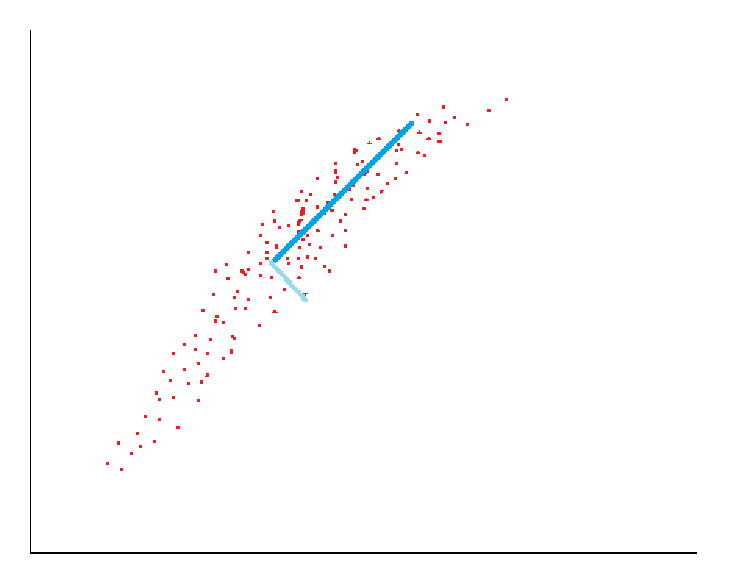
\includegraphics[width=0.6\linewidth]{pcaTwoDimensions}
\caption{Illustration of PCA.}
\label{fig:pcaTwoDimensions}
\end{figure}

Since we want to project the data from original orthogonal space to a new orthogonal space, we random select a point $p$ which will be considered the center of new orthogonal space. 
Let $x$ denotes the $n \times d$ data ($n$ is the samples count and $d$ is the feature dimension), $w$ denotes the $d \times dp$ normal orthogonal projection matrix, $w_{\_j}$ denotes the $kth$ coordinate vector from $p$, ${y_{ij}}$ denotes the coordinate point projected on $w_{\_j}$ of sample $x_{i\_}$ and ${y_{i\_}}$ denotes the new coordinate of sample $x_{i\_}$. Eq.~\ref{equ:pcaProjectVector} shows the computation of ${y_{i\_}}$.

\begin{equation}
\label{equ:pcaProjectVector}
\begin{aligned}
{y_{ij}} &= \left( {{x_{i\_}} - p} \right){w_{\_j}}^t\\
{y_{i\_}} &= \left( {{x_{i\_}} - p} \right)w\\
&= \left( {{x_{i\_}} - p} \right)w,\quad {w_{\_i}}^t{w_{\_j}} = \left\{ {\begin{array}{*{20}{c}}
{1,i = j}\\
{0,i \ne j}
\end{array}} \right.
\end{aligned}
\end{equation}

The energy on new orthogonal space can be described as Eq.~\ref{equ:pcaNewEnergy}. Matrix $m$ is a $d \times d$ positive semidefinite matrix.

\begin{equation}
\label{equ:pcaNewEnergy}
\begin{aligned}
energy &= \frac{1}{n}\sum\limits_{{\rm{i}} = 0}^{n - 1} {\sum\limits_{j = 0}^{dp - 1} {{{\left( {{y_{ij}} - {{\overline y }_{\_j}}} \right)}^2}} } \\
 &= \frac{1}{n}\sum\limits_{{\rm{i}} = 0}^{n - 1} {\parallel {y_{i\_}} - \overline y {\parallel ^2}} \\
 &= \frac{1}{n}\sum\limits_{{\rm{i}} = 0}^{n - 1} {\parallel \left( {{x_{i\_}} - p} \right)w - \frac{1}{n}\sum\limits_{j = 0}^{n - 1} {\left( {{x_{j\_}} - p} \right)w} {\parallel ^2}} \\
 &= \frac{1}{n}\sum\limits_{{\rm{i}} = 0}^{n - 1} {\parallel \left( {{x_{i\_}} - \overline x } \right)w{\parallel ^2}} \\
 &= \frac{1}{n}\sum\limits_{{\rm{i}} = 0}^{n - 1} {\sum\limits_{j = 0}^{{dp} - 1} {{{\left( {\left( {{x_{i\_}} - \overline x } \right){w_{\_j}}} \right)}^2}} } \\
 &= \frac{1}{n}\sum\limits_{{\rm{i}} = 0}^{n - 1} {\sum\limits_{j = 0}^{{dp} - 1} {{{\left( {\left( {{x_{i\_}} - \overline x } \right){w_{\_j}}} \right)}^2}} } \\
 &= \frac{1}{n}\sum\limits_{{\rm{i}} = 0}^{n - 1} {\sum\limits_{j = 0}^{{dp} - 1} {{w_{\_j}}^t{{\left( {{x_{i\_}} - \overline x } \right)}^t}\left( {{x_{i\_}} - \overline x } \right){w_{\_j}}} } \\
 &= \sum\limits_{j = 0}^{{dp} - 1} {{w_{\_j}}^t\left( {\frac{1}{n}\sum\limits_{i = 0}^{n - 1} {{{\left( {{x_{i\_}} - \bar x} \right)}^t}\left( {{x_{i\_}} - \bar x} \right)} } \right)} {w_{\_j}} \\
 &= \sum\limits_{j = 0}^{{dp} - 1} {{w_{\_j}}^t{m}{w_{\_j}}} 
\end{aligned}
\end{equation}

The optimization object of pca here can be shown as Eq.~\ref{equ:pcaOptimizationObjectMaxVariance}.

\begin{equation}
\label{equ:pcaOptimizationObjectMaxVariance}
\begin{aligned}
\mathop {\max }\limits_w J\left( w \right) &= \mathop {\max }\limits_w energy \\
&= \sum\limits_{j = 0}^{{dp} - 1} {{w_{\_j}}^t{m}{w_{\_j}}}\\
&s.t \quad \quad {w_{\_i}}^t{w_{\_j}} = \left\{ {\begin{array}{*{20}{c}}
{1,i = j}\\
{0,i \ne j}
\end{array}} \right.
\end{aligned}
\end{equation}

Base on Th.\ref{theo:maxminOptimization}, if we want to compute the maximum value of a function, we must to determine whether the function has upper bound. Fortunately, here the function has upper bound as shown in Eq.~\ref{equ:pcaEnergyUpperBound}.

\begin{equation}
\label{equ:pcaEnergyUpperBound}
\begin{aligned}
J\left( w \right) &= \sum\limits_{j = 0}^{{dp} - 1} {{w_{\_j}}^tm{w_{\_j}}} \\
 &= \sum\limits_{j = 0}^{{dp} - 1} {{w_{\_j}}^tm{w_{\_j}}} \\
 &= \sum\limits_{j = 0}^{{dp} - 1} {\sum\limits_{k = 0}^{d - 1} {\sum\limits_{l = 0}^{d - 1} {{w_{lj}}{m_{lk}}{w_{kj}}} } } \\
 &\le \sum\limits_{j = 0}^{{dp} - 1} {\sum\limits_{k = 0}^{d - 1} {\sum\limits_{l = 0}^{d - 1} {{m_{lk}}|{w_{lj}}||{w_{kj}}|} } } \\
 &\le \sum\limits_{j = 0}^{{dp} - 1} {\sum\limits_{k = 0}^{d - 1} {\sum\limits_{l = 0}^{d - 1} {{m_{lk}}} } } 
\end{aligned}
\end{equation}

Since the $energy$ has two constraints: normal and orthogonality. We eliminate the normal constraint in a equivalence way by Lagrange constant as shown in Eq.~\ref{equ:pcaLagrange}.

\begin{equation}
\label{equ:pcaLagrange}
\begin{aligned}
J(energy,\lambda ) &= energy - \sum\limits_{j = 0}^{j = {dp} - 1} {{\alpha ^j}({w_{\_j}}^t{w_{\_j}} - 1)} \\
\frac{{\partial J}}{{\partial {w_{\_j}}}} &= 2m{w_{\_j}} - 2{\alpha  ^j}{w_{\_j}} = 0\\
m{w_{\_j}} &= {\alpha ^j}{w_{\_j}}
\end{aligned}
\end{equation}

Let $u^i$ and $\lambda ^i$ denote the $ith$ eigenvector and eigenvalue respectively. We have the index vector $I$ as Eq.~\ref{equ:pcaIFront}. $I$ is a set and $I^j$ denotes the $jth$ vector element of $I$.

\begin{equation}
\label{equ:pcaIFront}
\begin{aligned}
m{u^i} &= {\lambda ^i}{u^i}\\
I &= \underbrace {[\forall i,...,\forall i]}_{{dp}},\quad I \in !order\& !repeat\\
\end{aligned}
\end{equation}

Then all the extreme point and their extreme value can be computed by Eq.~\ref{equ:pcaVarianceExtreme}.

\begin{equation}
\label{equ:pcaVarianceExtreme}
\begin{aligned}
w^j &= [{u^{{I^{j}_0}}},...,{u^{{I^{j}_{{dp} - 1}}}}]\\
energy^j &= {\lambda ^{{I^{j}_0}}} + ... + {\lambda ^{{I^{j}_{{dp} - 1}}}}
\end{aligned}
\end{equation}

We want to find the $w$ that corresponding the maximum energy. Obviously, the $dp$ eigenvectors which correspond to the maximum $dp$ eigenvalue constitute the transform matrix $w$. The $w$ also satisfy the constraint of orthogonality, according to Th.\ref{theo:loseConstraintProblem}, the $w$ is the final solution of PCA.  

Notice that, if $dp = d$, the projection matrix $w$ is not the only solution for maximizing projection variance, $w$ is just one of the solutions. In fact, all unit orthogonal weight are the solutions for maximizing projection variance (for any unit orthogonal weight, the energy will not changed after projection).

\subsection{Minimize Reconstruction Error}
Similarly, we random select a point $p$ which will be considered the center of new orthogonal space. 
Let $x$ denotes the $n \times d$ data ($n$ is the samples count and $d$ is the feature dimension), $w$ denotes the $d \times dp$ normal orthogonal projection matrix, $w_{\_j}$ denotes the $kth$ coordinate vector from $p$, ${y_{ij}}$ denotes the coordinate point projected on $w_{\_j}$ of sample $x_{i\_}$ and ${{\hat x}_{i\_}}$ denotes the reconstruction sample of $x_{i\_}$, as shown in Eq.~\ref{equ:pcaReconstructionVector}.

\label{sec:pcaMRE}
\begin{equation}
\label{equ:pcaReconstructionVector}
\begin{aligned}
{{\hat x}_{i\_}} &= p + \sum\limits_{j = 0}^{{dp} - 1} {{y_{ij}}{w_{\_j}}^t} \\
{x_{i\_}} &= p + \sum\limits_{j = 0}^{d - 1} {{y_{ij}}{w_{\_j}}^t} 
\end{aligned}
\end{equation}

Then the reconstruction error on $x$ can be described by Eq.~\ref{equ:pcaReconstructionError}. 

\begin{equation}
\label{equ:pcaReconstructionError}
\begin{aligned}
e &= \frac{1}{n}{\sum\limits_{i = 0}^{n - 1} {\parallel {{\hat x}_{i\_}} - {x_{i\_}}\parallel } ^2}\\
 &= \frac{1}{n}{\sum\limits_{i = 0}^{n - 1} {\parallel \sum\limits_{j = {dp}}^{d - 1} {{y_{ij}}{w_{\_j}}^t} \parallel } ^2}\\
 &= \frac{1}{n}\sum\limits_{i = 0}^{n - 1} {\left( {\sum\limits_{j = {dp}}^{d - 1} {{y_{ij}}{w_{\_j}}^t} } \right)} {\left( {\sum\limits_{j = {dp}}^{d - 1} {{y_{ij}}{w_{\_j}}^t} } \right)^t}\\
 &= \frac{1}{n}\sum\limits_{i = 0}^{n - 1} {\sum\limits_{j = {dp}}^{d - 1} {{y_{ij}}^2} } \\
 &= \frac{1}{n}\sum\limits_{i = 0}^{n - 1} {\sum\limits_{j = {dp}}^{d - 1} {{{\left( {\left( {{x_i} - p} \right){w_{\_j}}} \right)}^2}} } \\
 &= \frac{1}{n}\sum\limits_{i = 0}^{n - 1} {\sum\limits_{j = {dp}}^{d - 1} {{w_{\_j}}^t\left( {{x_i} - p} \right){{\left( {{x_i} - p} \right)}^t}{w_{\_j}}} } 
\end{aligned}
\end{equation}

The optimization object of pca here can be shown as Eq.~\ref{equ:pcaOptimizationObjectMinReError}. Obviously, the optimization object has lower bound which equals to 0.
\begin{equation}
\label{equ:pcaOptimizationObjectMinReError}
\begin{aligned}
&\mathop {\min }\limits_{{w_{0,...,{dp} - 1}}} J\left( w \right) = \mathop {\min }\limits_{{w_{0,...,{dp} - 1}}} e \in \mathop {\min }\limits_w e\\
&s.t \quad \quad {w_{\_i}}^t{w_{\_j}} = \left\{ {\begin{array}{*{20}{c}}
{1,i = j}\\
{0,i \ne j}
\end{array}} \right.
\end{aligned}
\end{equation}

Since the $e$ has two constraints: normal and orthogonality. We eliminate the normal constraint in a equivalence way by Lagrange constant as Eq.~\ref{equ:pcaConstraintFunction}. Eq.~\ref{equ:pcaDerivationToP} and Eq.~\ref{equ:pcaDerivationToW} show the solution procedure for $p$ and $w$.

\begin{equation}
\label{equ:pcaConstraintFunction}
\begin{aligned}
J\left( {e,\lambda } \right) = e + \sum\limits_{k = {dp}}^{d - 1} {{a ^k}\left( {{w_{\_j}}^t{w_{\_j}} - 1} \right)} 
\end{aligned}
\end{equation}

\begin{equation}
\label{equ:pcaDerivationToP}
\begin{aligned}
\frac{{\partial J}}{{\partial p}} &= \frac{{\partial e}}{{\partial p}}\\
 &= \frac{{\partial \frac{1}{n}\sum\limits_{i = 0}^{n - 1} {\sum\limits_{j = {dp}}^{d - 1} {{w_{\_j}}^t\left( {{x_i} - p} \right){{\left( {{x_i} - p} \right)}^t}{w_{\_j}}} } }}{{\partial p}}\\
 &= \frac{{\partial \frac{1}{n}\sum\limits_{i = 0}^{n - 1} {\sum\limits_{j = {dp}}^{d - 1} {{{\left( {\left( {{x_i} - p} \right){w_{\_j}}} \right)}^2}} } }}{{\partial p}}\\
 &= \frac{{\partial \frac{1}{n}\sum\limits_{i = 0}^{n - 1} {\sum\limits_{j = {dp}}^{d - 1} {{{\left( {\left( {{x_i} - p} \right){w_{\_j}}} \right)}^2}} } }}{{\partial \frac{1}{n}\left( {{x_i} - p} \right)}}\frac{{\partial \left( {{x_i} - p} \right)}}{{\partial p}}\\
 &= \frac{2}{n}\sum\limits_{i = 0}^{n - 1} {\sum\limits_{j = {dp}}^{d - 1} {\left( {{x_i} - p} \right)w{}_{\_j}{w_{\_j}}^t} } \left( { - 1} \right)\\
 &=  - \frac{2}{n}\left( {d - {dp}} \right)\sum\limits_{i = 0}^{n - 1} {\left( {{x_i} - p} \right)}  \\
 &= 0 \\
 &\Rightarrow p = {\bar x}
\end{aligned}
\end{equation}

\begin{equation}
\label{equ:pcaDerivationToW}
\begin{aligned}
\frac{{\partial J}}{{\partial {w_{\_j}}}} &= \frac{{\partial \frac{1}{n}\sum\limits_{i = 0}^{n - 1} {\sum\limits_{j = {dp}}^{d - 1} {{w_{_{\_j}}}^t{{\left( {{x_i} - \bar x} \right)}^t}\left( {{x_i} - \bar x} \right){w_{\_j}}} } }}{{\partial {w_{\_j}}}} - \frac{{\partial \sum\limits_{j = {dp}}^{d - 1} {{a^j}\left( {{w_{\_j}}^t{w_{\_j}} - 1} \right)} }}{{\partial {w_{\_j}}}}\\
 &= \frac{{\partial \sum\limits_{j = {dp}}^{d - 1} {{w_{_{\_j}}}^t\left( {\frac{1}{n}\sum\limits_{i = 0}^{n - 1} {{{\left( {{x_i} - \bar x} \right)}^t}\left( {{x_i} - \bar x} \right)} } \right){w_{\_j}}} }}{{\partial {w_{\_j}}}} - \frac{{\partial \sum\limits_{j = {dp}}^{d - 1} {{a^j}\left( {{w_{\_j}}^t{w_{\_j}} - 1} \right)} }}{{\partial {w_{\_j}}}}\\
 &= \frac{{\partial \sum\limits_{j = {dp}}^{d - 1} {{w_{_{\_j}}}^tm{w_{\_j}}} }}{{\partial {w_{\_j}}}} - \frac{{\partial \sum\limits_{j = {dp}}^{d - 1} {{a^j}\left( {{w_{\_j}}^t{w_{\_j}} - 1} \right)} }}{{\partial {w_{\_j}}}}\\
 &= 2m{w_{\_j}} - 2{a^j}{w_{\_j}}\\
 &= 0\\
 &\Rightarrow m{w_{\_j}} = {a^j}{w_{\_j}}
\end{aligned}
\end{equation}

Let $u^i$ and $\lambda ^i$ denote the $ith$ eigenvector and eigenvalue respectively. We have the index vector $I$ as Eq.~\ref{equ:pcaIBack}. $I$ is a set and $I^j$ denotes the $jth$ vector element of $I$.

\begin{equation}
\label{equ:pcaIBack}
\begin{aligned}
m{u^i} &= {\lambda ^i}{u^i}\\
I &= \underbrace {[\forall i,...,\forall i]}_{{d - dp}},\quad I \in !order\& !repeat\\
\end{aligned}
\end{equation}

Then all the extreme point and their extreme value can be computed by Eq.~\ref{equ:pcaErrorExtreme}.

\begin{equation}
\label{equ:pcaErrorExtreme}
\begin{aligned}
w^j_{dp,...,d - 1} &= [{u^{{I^j_{dp}}}},...,{u^{{I^j_{{d - 1}}}}}]\\
e^j &= {\lambda ^{{I_0}}} + {\lambda ^{{I^j_1}}} + ... + {\lambda ^{{I^j_{{dp} - 1}}}}
\end{aligned}
\end{equation}

We want to find the $w_{dp,...,d - 1}$ that corresponding the minimum reconstruction error. Obviously, the $d - dp$ eigenvectors which corresponding to the minimum $d - dp$ eigenvalue constitute the transform matrix $w^j_{dp,...,d - 1}$. So the projection matrix $w_{0,...dp - 1}$ is composed by the $dp$ eigenvectors (in unordered type) corresponding the maximum $dp$ eigenvalue. The $w_{0,...dp - 1}$ also satisfy the constraint of orthogonality, according to Th.\ref{theo:loseConstraintProblem}, the $w_{0,...dp - 1}$ is the final solution of PCA.  

Notice that, the difference of optimization theory between maximizing projection variance and minimizing reconstruction error is that the center point of projection axis can be any point in the former while it must be the center of original point in the latter. 

\subsection{PCA Process}
\begin{itemize}
  \item Subtract data (if don't reconstruct, you can subtract any point),
  \item Computer covariance matrix,
  \item Computer eigenvector and eigenvalue,
  \item Select the eigenvectors corresponding the maximum $dp$ eigenvalues or the sum of maximum eigenvalues over the $ratio\%$ of total eigenvalues.
\end{itemize}

\subsection{PCA Conclusion}
As our inference in Sec.\ref{sec:pcaMPV} and Sec.\ref{sec:pcaMRE}, the project matrix $w$ is composed of the eigenvectors. The covariance matrix of the data after projecting $m_y$ can be computed by Eq.~\ref{equ:pcaCovMatrixAfterProjecting}.

\begin{equation}
\label{equ:pcaCovMatrixAfterProjecting}
\begin{aligned}
{m_y} &= \frac{1}{n}\sum\limits_{i = 0}^{n - 1} {{{\left( {{y_{i\_}} - \bar y} \right)}^t}\left( {{y_{i\_}} - \bar y} \right)} \\
 &= \frac{1}{n}\sum\limits_{i = 0}^{n - 1} {{{\left( {\left( {{x_{i\_}} - \bar x} \right)w} \right)}^t}\left( {{x_{i\_}} - \bar x} \right)w} \\
 &= \frac{1}{n}\sum\limits_{i = 0}^{n - 1} {{w^t}{{\left( {{x_{i\_}} - \bar x} \right)}^t}\left( {{x_{i\_}} - \bar x} \right)w} \\
 &= {w^t}{m_x}w
\end{aligned}
\end{equation}
Where $m_x$ is the covariance matrix of the original data. The result of $m_y$ is a diagonal matrix where the diagonal entries are the eigenvalues of $m_x$ 
corresponding the eigenvectors in $w$.
If the dimension of $w$ is $d$, the energy after projecting is as same as the energy in original axis.
Since the $m_y$ is a diagonal matrix, so the new data projected in new orthogonal space is uncorrelated in each two dimensions.

For any two correlative dimensions, after eliminate relativity, one projection axis will along the main distributed directional in data space and the energy on this axis will greater than the other projective axis. The more correlative, the bigger difference of energy.


\chapter{Application}
\section{Classify Problem}
A classify problem consider four elements, expectation, data, feature and model.
\subsection{Expectation}
\subsection{Data}
Data is divided into balanced data and unbalanced data. In this section, we only consider the non-redundant data since we can always generate a balanced data through re-sampling the less part of data or sub-sampling the major part of data. The degree of balance of training data is as same as the testing data. For object detection problem, the data is unbalanced. The positive objects can be consider as rare object while the number of negative objects are tremendous. Unbalanced data will bring some predicaments for many learning models, such as decision tree, neural work and so on.
\subsection{Feature}
\subsection{Model}
\subsection{Brief Summary}

\section{Object Detection}
\subsection{Sliding Window Based Method}
The Sliding window based methods are frequently-used in object detection since the sliding window mechanism could produce infinite candidate object regions. It is easily to get high object detect ratio (DR) by adopting sliding window (multiple sliding window formally).

There are two types of sliding window mechanism. One is multiple scales of sliding windows and the source image is single. The other one is multiple scales of source image and the size of sliding windows are constant. Normally, the latter is more appropriate than the former. 
From the aspect of feature representation, which is the main difference between the two types, the total cost time of feature representation $T$ can be calculated by $\sum_{i = 1}^{n} t(i)$, where $t(i)$ indicates the cost time of feature representation for $ith$ window. In most cases, the $t(i)$ is at least linear (even square) complexity for the $ith$ window size. If we exploit the former, the $T$ is likely to be very large due to the big window sizes in multiple scales. However, the $T$ will be lesser in latter type since the sliding window sizes are constant and the extra cost time of scale multiple images is lightly tolerant in most times. 
So we can summarize the two types as follower, if $t$ is very litter (like the harr feature only need several times of multiplicative) or the cost time of scaling source image are obviously time consuming, we adopt the former. Otherwise the latter is best choice.

A general sliding window based method is shown in Fig.~.

\subsection{Training Dataset for Sliding Window Methods}
Since the sliding window (or source image) need to be scaled and moved over the source image (or the scaled image), some object may not be perfectly matched with the sliding window.
Here we discuss the type of multiple scales of sliding windows, since the training samples for the two types are the same.
Usually, the training dataset only contains the ground truth rectangles that match the object accurately. However, the feature extracted from unmatched sliding window may be obviously different from the feature extracted from the ground truth rectangle, this will bring the difficult judgement for the learned model.
Hence, we may need to generate the augmented training dataset to handle the imperfectly matched cases when the stride ratio and scaled stride ratio are big.

Specifically, for an object in image, let $x, y$ denote its left and top position, $w, h$ denote its width and height (sliding window), $r, r_{*h}$ denote the stride ratio to sliding width, $g, g_{*h}$ denote the scaled stride ratio. 
We first discuss the case that sliding window size is same as the object. 
As shown in Fig.~\ref{fig:sliding_window_position_match}, the sliding window may not be match perfectly with the object. 
Hence we need to drawn the augmented samples in the range of $\left[ {l \le x < l + wr} \right)$ or $\left( {l < x \le l + wr} \right]$ in horizontal direction and as the same strategy in vertical direction (in fact the drawn is implemented by drawn the top-left point, the drawn region of top-left point is a rectangle as shown in Fig.~\ref{fig:sliding_window_position_drawn_region}).
Then we discuss the unmatched cases of sliding window size and object size, as shown in Fig.~\ref{fig:sliding_window_size_match}. 
We need to drawn the augmented samples in the range of $\left[ {{w_{*s}} < w \le {w_{*s}} + {w_{*s}}g} \right)$ or $\left( {{w_{*s}} < w \le {w_{*s}} + {w_{*s}}g} \right]$, for width as the same strategy for height. 

\begin{figure}
\centering
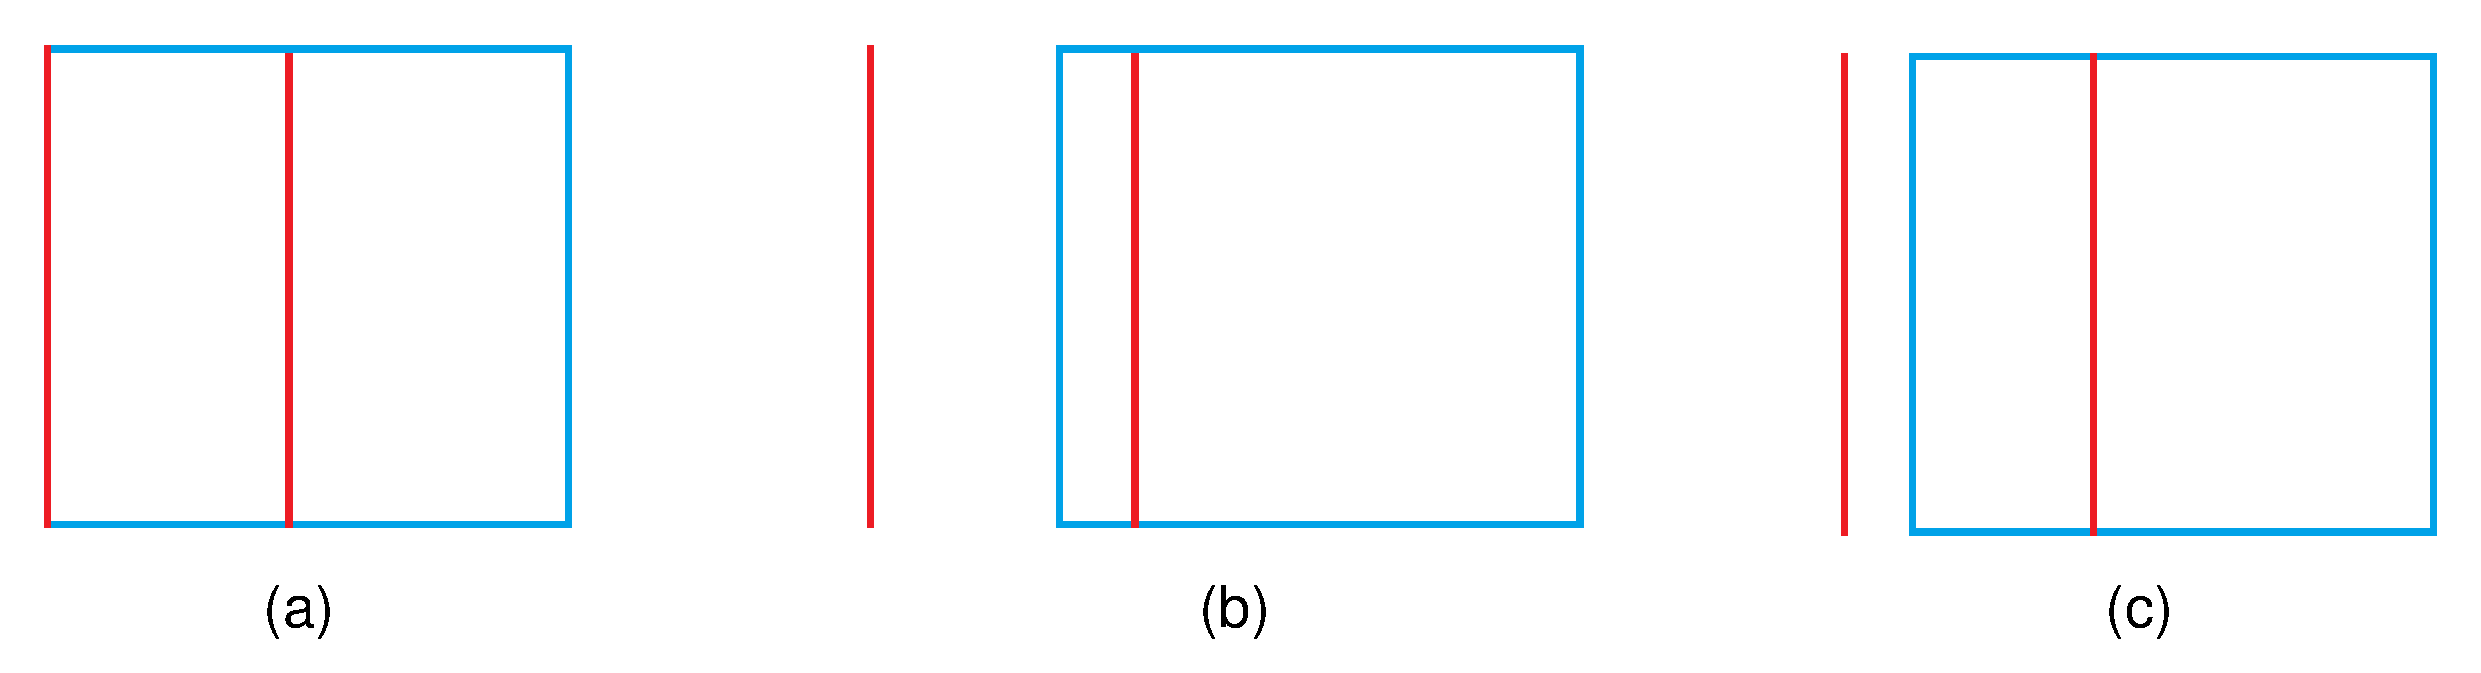
\includegraphics[width=0.6\linewidth]{sliding_window_position_match}
\caption{Illustration of the matching cases of the sliding window position with object.(a) perfect matching, (b) and (c) imperfect matching. Blue bounding boxes indicate the object window while red lines indicate the left sides of sliding window.}
\label{fig:sliding_window_position_match}
\end{figure}

\begin{figure}
\centering
\includegraphics[width=0.2\linewidth]{sliding_window_position_drawn_region}
\caption{Illustration of the drawn region (green bounding box) of top-left point of mismatching window position.}
\label{fig:sliding_window_position_drawn_region}
\end{figure}

\begin{figure}
\centering
\includegraphics[width=0.2\linewidth]{sliding_window_size_match}
\caption{Illustration of the mismatching cases of the sliding window size with object.}
\label{fig:sliding_window_size_match}
\end{figure}

For the training samples, we first drawn the augmented samples of unmatched window position in the range of $\left[ {l \le x < l + wr} \right), \left[ {t \le y < t + hr_{*h}} \right)$ (the top-left point of drawn samples). 
Then we drawn augmented samples of unmatched window size from the augmented samples of unmatched window position and the original training samples by expand the width and height in both two side (left and right for width, top and bottom for height) in the size range of 

\begin{displaymath}
\left[{w_{*s}} < w \le {w_{*s}} + {w_{*s}}r\right), \left[{h_{*s}} < h \le {h_{*s}} + {h_{*s}}r\right)
\end{displaymath}
simultaneously.

Usually, we let $x = l + \frac{{wr}}{2}, y = t + \frac{{hr_{*h}}}{2}$ (the drawn samples are most closed to true samples), so the drawn region of top-left position for unmatched window position is 

\begin{displaymath}
\left[ {x- \frac{{wr}}{2} \le x < x + \frac{{wr}}{2}} \right), \left[y - \frac{{h{r_{*h}}}}{2} \le y < y + \frac{{h{r_{*h}}}}{2}\right)
\end{displaymath}
Similarly, we let 

\begin{displaymath}
w = {w_{*s}} + \frac{{1 + g}}{2}, h = {h_{*s}} + \frac{{1 + g_{*h}}}{2}
\end{displaymath}
, the drawn region of size for unmatched window size is 

\begin{displaymath}
\left[\frac{{2w}}{{2 + g}} < w \le \frac{{2w\left( {1 + g} \right)}}{{2 + g}}\right), \left[\frac{{2h}}{{2 + g_{*h}}} < h \le \frac{{2h\left( {1 + g_{*h}} \right)}}{{2 + g_{*h}}}\right)
\end{displaymath}

The big stride ratio and scaled stride ratio will reduce the windows number while require the more augmented training samples and some augmented training sample may are obviously different from the true training samples.
Hence we set the stride ratio of width and height to $0.25$, scaled stride ratio of width and height to $0.4$.
Then the drawn region of top-left position for unmatched window position is $\left[ {x- \frac{{w}}{8}} \le x < x + \frac{{w}}{8} \right), \left[y - \frac{{h}}{8} \le y < y + \frac{{h}}{8}\right)$. 
The drawn region of size for unmatched window size is $\left[\frac{{2w}}{{2 + r}} < w \le \frac{{2w\left( {1 + r} \right)}}{{2 + r}}\right), \left[\frac{{2h}}{{2 + r_{*h}}} < h \le \frac{{2h\left( {1 + r_{*h}} \right)}}{{2 + r_{*h}}}\right)$.

\subsection{Component Based Method}
\section{Object Recognition}
%===========================================================
\bibliographystyle{splncs}
\bibliography{egbib}

%this would normally be the end of your paper, but you may also have an appendix
%within the given limit of number of pages
\end{document}
